\documentclass[12pt, titlepage, openany]{amsbook}

%%% Comment or uncomment any or all of the following packages as
%%% necessary. TeX will run faster the fewer packages it has to load... 
%%% You can/should load any other packages you need, but be aware that
%%% packages can and do modify style parameters, some packages are
%%% incompatible with other packages, and some packages have requirements
%%% about whether or not they have to be loaded before or after other
%%% packages.  

%%% The standard AMS math packages
\usepackage{amsmath, amsfonts, amssymb, amsthm, esint, subfig, textcomp}


%%% For diagrams and "pics." Tikz is probably a better choice...
\usepackage[all]{xy}

%%% For hyperrefs, breaklinks might cause problems (or not really help with
%%% long hyperrefs...) 
% Uncomment the following two lines and change "allcolors=black" to
% "allcolors=untgreen" to get UNT branded green hyperlinks
\usepackage{color}
\definecolor{untgreen}{RGB}{5,144,51}
%\usepackage{aliascnt} 
\usepackage[colorlinks, linktocpage, allcolors=untgreen,%
breaklinks,pagebackref=true]{hyperref}


%%% One option for complicated tables and arrays. The array package is used
%%% in 
\usepackage{array} 

%%% One option for including graphics
\usepackage{graphicx, epstopdf}
\graphicspath{
    {pics/chapter1/}
    {pics/chapter2/}
    {pics/chapter3/}
    {pics/chapter4/}
    {pics/chapter5/}
    {pics/appendix/}
}


%%% For professional tables (as in the appendix), comment out if there are
%%% no tables
\usepackage{booktabs, caption, multicol}


%%% Uncomment the following line to get the computer modern equivalent of
%%% ``arial.'' Probably doing so will alter line breaks throughout the
%%% document...
%\usepackage{cmbright}
%%% Uncomment the following line if line spacing is funky when the last line
%%% is uncommented.
%\usepackage[standard-baselineskip]{cmbright}

%%% Cleveref plays nicely with amsthm and likes to be the last package to be
%%% loaded
\usepackage[capitalise, nameinlink]{cleveref}


%%%%%%%%%%% preamble stuff ...
%%% This loads the main style file.
%%%%%%%%%%%%%%%%%%%%%%%%%%%%%%%%%%%%%%%%%%%%%%%%%%%%%%%%%%%%%%
%%% \makeatletter ...
%%%%%%%%%%%%%%%%%%%%%%%%%%%%%%%%%%%%%%%%%%%%%%%%%%%%%%%%%%%%%%
%%% \makeatletter is neneeded to be able to access some of the more
%%% primitive macros below.
\makeatletter

%%%%%%%%%%%%%%%%%%%%%%%%%%%%%%%%%%%%%%%%%%%%%%%%%%%%%%%%%%
%%% Modifying amsbook.cls
%%%%%%%%%%%%%%%%%%%%%%%%%%%%%%%%%%%%%%%%%%%%%%%%%%%%%%%%%%
%%%
%%% The following supersedes the amsbook.cls class file.
%%%
%%%
%%% Page Dimensions
%%%
%%% \voffset shifts the whole ``page'' up (negative) or down (positive) on
%%% the paper.
%%%
%%% \topmargin is the distance from 1'' down on the page (assuming
%%% \voffset=0pt) and the top of the headline.
%%%
%%% \headheight is the height of the headline above its baseline
%%%
%%% \headsep is the distance from the baseline of the headline to the top of
%%% the page body.
%%%
%%% The first baseline for a line on the page body is: 1'' + \topmargin +
%%% \headheight + \headsep + point size (12pt)
%%%
%%% \textheight is the goal distance from the top of the first line of text
%%% to the baseline of the last line of text.
%%%
%%% If TeX can't get a baseline exactly \texheight from the top of the first
%%% line of text, the first line stays put and space is added
%%% ``more-or-less'' evenly between each line of text on the page.
%%%
%%% \footsep is the distance from the bottom of the body of the text on the
%%% page to the baseline of the footline.
%%%
%%% To get page numbers .5in from the bottom of the page for 8 1/2 x 11 
%%% paper, we need:
%%% 1'' + \topmargin + \headheight + \headsep + \textheight + \footskip
%%% = 10.5in 
%%% Mess with \textheight and \footskip to change the size of the
%%% body of the page and the distance from the last baseline to the
%%% baseline of the footline. To move the whole shebang up, using
%%% \voffset is probably safest.
\setlength{\voffset}{0pt}
\setlength{\topmargin}{0pt}
\setlength{\headheight}{0pt}
\setlength{\headsep}{0pt}
\setlength{\textheight}{9in}
\setlength{\footskip}{.5in}

%%% \hoffset is the horizontal analog of \voffset, positive to shift right,
%%% negative to shift left
%%%
%%% \oddsidemargin is the left hand margin minus 1'' on odd numbered
%%% pages.
%%% \evensidemargin is the left hand margin minus 1'' on even numbered
%%% pages. 
%%%
%%% \textwidth is the width of the body of the text on the page.
\setlength{\hoffset}{0pt}
\setlength{\evensidemargin}{0pt}
\setlength{\oddsidemargin}{0pt}
\setlength{\textwidth}{6.5in}

%%% This changes the standard line breaking penalties back to the plain TeX
%%% standard which is much less stringent than for AMS styles
\widowpenalty=150 
\clubpenalty=150
\brokenpenalty=100
\displaywidowpenalty=50

%%% ``Double'' spacing can be achieved by either of the following -- the
%%% LaTeX book recommends \baselinestretch and some online source says
%%% \linespread is to draconian.
\renewcommand{\baselinestretch}{1.66}
%\linespread{1.66}

%%% Half inch \parindent per TGS style ... this hurts....
\setlength{\parindent}{.5in}

%%% A feeble and probably futile attempt at adding some bonus interline glue
%%% to help reduce underfull hboxes when pages are typeset (jmd 6-11-2013)
\lineskip=1pt plus 1pt
\setlength{\parskip}{0pt plus 2pt}


%%%%%%%%%%%%%%%%%%%%%%%%%%%%%%%%%%%%%%%%%%%%%%%%%%%%%%%%%
%%% This is the page style, no headline, footline contains the page number,
%%% which is centered.
\pagestyle{plain} 

%%% AMS document classes seem to like scriptsize page numbers. Here is a
%%% fix.
\def\ps@plain{\ps@empty%
  \def\@oddfoot{\normalfont \hfil\textnormal{\thepage}\hfil}%
  \let\@evenfoot\@oddfoot}
%%% For the other page styles... 
\renewcommand{\@evenfoot}{\hfil\textnormal{\thepage}\hfil}%
\renewcommand{\@oddfoot}{\@evenfoot}%


%%%%%%%%%%%%%%%%%%%%%%%%%%%%%%%%%%%%%%%%%%%%%%%%%%%%%%%%%
%%% These need to be redefined to disable the usual AMS book style which
%%% inserts blank pages all over creation. To get blank pages between the
%%% frontmatter, mainmatter, and backmatter, replace \clearpage with
%%% \cleardoublepage.
\def\frontmatter{\clearpage\pagenumbering{roman}}
\def\mainmatter{\clearpage\pagenumbering{arabic}}
\def\backmatter{\if@openright\clearpage\else\clearpage\fi
  \let\chaptername\relax} 


%%%%%%%%%%%%%%%%%%%%%%%%%%%%%%%%%%%%%%%%%%%%%%%%%%%%%%%%%
%%% Here's where the titlepage magic happens...
%%%
\renewcommand\titlepage{%
  \clearpage
  \thispagestyle{empty}\setcounter{page}{0}}
\renewcommand\maketitle{\par
  \@topnum\z@ % this prevents figures from falling at the top of page 1
  \begingroup
  \@maketitle
  \endgroup
  \c@footnote\z@
  \def\do##1{\let##1\relax}%
  \do\maketitle \do\@maketitle \do\title \do\@xtitle \do\@title
  \do\author \do\@xauthor \do\address \do\@xaddress
  \do\email \do\@xemail \do\curraddr \do\@xcurraddr
  \do\dedicatory \do\@dedicatory \do\thanks \do\thankses
  \do\keywords \do\@keywords \do\subjclass \do\@subjclass
}
\renewcommand*{\title}[1]{\gdef\@title{\uppercase {#1}}}
\renewcommand\@maketitle{%
  \clearpage \thispagestyle{empty}%
  \begingroup \topskip\z@skip \null
    \vfil 
    \begingroup \centering \@title\par 
      \def\and{\par\medskip}\centering
      \mdseries\authors\par\bigskip 
    \endgroup 
    \vfill
    \begingroup \centering
      \ifx\@empty\degree \else  \@degree\par \fi 
      \vfill 
      \ifx\@empty\degreedate \else \@degreedate\par  \fi 
    \endgroup
    \vfill 
    \begingroup
    %%% Back in the day (January 2013), the approved block was right
    %%% justified. Now, the approved block is supposed to start half way
    %%% across the page... (jmd 6-11-2013)
    %  \parindent=0pt 
    %  \raggedleft
      \parindent= 3.25in
    %% The following sets up single space for the list of approvers jmd
    %% 6/2012 
      \renewcommand{\baselinestretch}{1} \normalsize
      \begin{tabular}{l}
        APPROVED: \vspace{.75em} \\ \noalign{\smallskip} \@approved
      \end{tabular}\par
    \endgroup
  \endgroup
}
%%%
\newcommand\degree[1]{\def\@degree{#1}}
\let\@degree=\@empty
\newcommand\degreedate[1]{\def\@degreedate{UNIVERSITY OF NORTH TEXAS\\
    #1}}
\let\@degreedate=\@empty
%%%
\newcommand\approved[1]{\def\@approved{#1}}
\let\@approved\@empty


%%%%%%%%%%%%%%%%%%%%%%%%%%%%%%%%%%%%%%%%%%%%%%%%%%%%%%%%%
%%% The numbering commands 
%%%
%%% Chapters and sections are in arabic numerals and sections are numbered
%%% as chapter.section.  
\renewcommand{\thechapter}{\arabic{chapter}}
\renewcommand{\thesection}{\thechapter.\arabic{section}}
\setcounter{secnumdepth}{3}
\setcounter{tocdepth}{3}

%%% This redefines the \section command so that it's flush left and the font
%%% is the normal text font.
\renewcommand\section{\@startsection{section}{1}%
  \z@{.35\linespacing\@plus\linespacing}{.25\linespacing}%
  {\normalfont}}

%%% This redefines the \subsection command so that it's flush left and
%%% in the normal font.
\renewcommand\subsection{\@startsection{subsection}{2}%
  \z@{.35\linespacing\@plus.7\linespacing}{.25\linespacing}%
  {\normalfont}}

%%% This redefines the \subsubsection command so that it's flush left and
%%% in the normal font.
\renewcommand\subsubsection{\@startsection{subsubsection}{3}%
  \z@{.35\linespacing\@plus.7\linespacing}{.25\linespacing}%
  {\normalfont}}


%%%%%%%%%%%%%%%%%%%%%%%%%%%%%%%%%%%%%%%%%%%%%%%%%%%%%%%%%
%%% These redefine how chapters are started and the table of contents
%%% entries are written... 
%%%
%%% \@makechapterhead is for numbered chapters (called with \chapter{MY
%%% CHAPTER}). \@makeshapterhead (called with \chapter*{MY CHAPTER WITH
%%% NO CHAPTER NUMBER}) is for unnumbered chapters, such as an appendix (if
%%% there's only one). For example, \chapter*{Appendix} would be a great way
%%% to start an appendix. If there's more than one appendix, then look up
%%% how the \appendix command affects chapter numbering...
\renewcommand\@makechapterhead[1]{\global \topskip 44pt\relax%
  %%% 44pt seems to be the secret number to get the baseline of CHAPTER X to
  %%% be 1in + Cap Height from the top of the page
  \begingroup%
  \fontsize{\@xivpt}{18}\centering%
  \ifnum\c@secnumdepth>\m@ne%
    \leavevmode \hskip-\leftskip%
    \rlap{\vbox to\z@{\vss%
      \centerline{\normalsize\mdseries%
        \uppercase\@xp{\chaptername}\enspace\thechapter}%
      \vskip 3pc}}\hskip\leftskip\fi%
  \uppercase{#1}\par \endgroup%
  \skip@34\p@ \advance\skip@-\normalbaselineskip%
  \vskip\skip@}
\renewcommand\@makeschapterhead[1]{\global \topskip 10pt\relax%
  %%% Tricky.... numbered chapters have an extra line at the top -- CHAPTER
  %%% X -- and this line is set using the funky \vbox above, unnumbered
  %%% chapters don't have this bonus line, so topskip goes back to its normal
  %%% value and everything is cool (jmd 8/5/2014)
  \begingroup%
  \fontsize{\@xivpt}{18}\centering%
  \uppercase{#1}\par \endgroup%
  \skip@34\p@ \advance\skip@-\normalbaselineskip%
  \vskip\skip@}
\def\@chapter[#1]#2{\refstepcounter{chapter}%
  \ifnum\c@secnumdepth<\z@ \let\@secnumber\@empty
  \else \let\@secnumber\thechapter \fi
  \typeout{\chaptername\space\@secnumber}%
  \def\@toclevel{0}%
  \ifx\chaptername\appendixname \@tocwriteb\tocappendix{chapter}{#2}%
%%% The next line has the efffect of ignoring the toc chapter title option
%%% in the \chapter command. Presumably this is an AMS style "feature."
%%% Change #2 to #1 to (hopefully) get the default LaTeX behavior. (jmd
%%% 2/2017, based on an observation by William Cherry)
  \else \@tocwriteb\tocchapter{chapter}{#2}\fi

%  \else \@tocwriteb\tocchapter{chapter}{#2}\fi
  \chaptermark{#1}%
  \@makechapterhead{#2}\@afterheading}
\def\@schapter#1{\typeout{#1}%
  \let\@secnumber\@empty
  \def\@toclevel{0}%
  \ifx\chaptername\appendixname \@tocwriteb\tocappendix{chapter}{#1}%
  \else \@tocwriteb\tocchapter{chapter}{#1}\fi
  \chaptermark{#1}%
  \@makeschapterhead{#1}\@afterheading}

%%% Bibliographies + appendices in amscls were/are a bit funky. Plus, TGS
%%% style for appendices is different than the TGS style for chapters, so
%%% the usual \chapter ain't right in an appendix. The following redefines
%%% the \appendix command so that when appendices start with \appchapter,
%%% for numbered appendices, like, say, if there is more than one, or
%%% \appchapter*, in case there is only one appendix, the "chapter" title is
%%% centered on a page it gets all to itself. Probably there are still bugs
%%% in this code. (jmd 6-11-2013)
\renewcommand\appendix{\par
  \c@chapter\z@ \c@section\z@
  \let\chaptername\appendixname
  \renewcommand{\thechapter}{\@Alph\c@chapter}
  \newcommand\appchapter{\clearpage \thispagestyle{plain}%
       \null\vfill \markboth{}{}\secdef\@appchapter\@appschapter}}
\def\@appchapter[#1]#2{\refstepcounter{chapter}%
  \ifnum\c@secnumdepth<\z@ \let\@secnumber\@empty \else
  \let\@secnumber\thechapter \fi \typeout{\chaptername\space\@secnumber}%
  \def\@toclevel{0}%
  \ifx\chaptername\appendixname \@tocwriteb\tocappendix{chapter}{#2}%
  \else \@tocwriteb\tocchapter{chapter}{#2}\fi
  \chaptermark{#1}%
  \begingroup\centering
  \ifnum \c@secnumdepth >-2\relax {\chaptername\ \thechapter} \vskip 12\p@
  \fi #2\vfill\endgroup \newpage\thispagestyle{plain}%%% next line added...
  \renewcommand{\thetable}{\Alph{chapter}.\arabic{table}}
  \renewcommand{\thefigure}{\Alph{chapter}.\arabic{figure}}}
% The starred version needs a little extra tweaking in order to get the toc
% and cross-references to come out right... (jmd 3/2017)
\def\@appschapter#1{\typeout{#1}%
  \refstepcounter{chapter}
  \let\@secnumber\thechapter
  \def\@toclevel{0}%
  \@tocwriteb\tocsappendix{chapter}{#1}%
  \chaptermark{#1}%
  \begingroup\centering
  \ifnum \c@secnumdepth >-2\relax {\chaptername} \vskip 12\p@
  \fi #1\vfill\endgroup \newpage\thispagestyle{plain}%%% next line added...
  \renewcommand{\thetable}{A.\arabic{table}}
  \renewcommand{\thefigure}{A.\arabic{figure}}}

%%% Make the lists of tables, list of figures, contents, chapter, appendix,
%%% and bibliography all uppercase.
\renewcommand\contentsname{TABLE OF CONTENTS}
\renewcommand\listtablename{LIST OF TABLES}
\renewcommand\listfigurename{LIST OF FIGURES}
\renewcommand\chaptername{CHAPTER}
\renewcommand\appendixname{APPENDIX}
\renewcommand\bibname{\myrefbibname}

%%% TOC, LOT, and LOF bits and bobs
%%% Note that AMS style is to have section/table/figure... numbers in the
%%% TOC/LOT/LOF followed by a .

%%% Add "Page" at the top of the column of page numbers (jmd 6-29-2013)
\def\@starttoc#1#2{%
  \begingroup 
  \setTrue {#1}%
  \let \secdef \@gobbletwo \chapter 
  \let \@secnumber \@empty 
  \ifx \contentsname #2%
  \else \@tocwrite {chapter}{#2}\fi
  \typeout {#2}\@xp \chaptermark \@xp {#2}%
  \@makeschapterhead {#2}\@afterheading 
  \hbox to \hsize{\hfill Page} % per UNT style ...
  \parskip\z@skip 
  \makeatletter 
  \@input {\jobname .#1}%
  \if@filesw 
    \@xp \newwrite \csname tf@#1\endcsname 
    \immediate \@xp \openout \csname tf@#1\endcsname \jobname .#1\relax 
  \fi 
  \global \@nobreakfalse \endgroup 
  \newpage 
}

%%% Fuss with the spacing/indentation TOC lines (jmd 6-29-2013)
%%%
%%% Chapters and appendices (heading level 1 in TGS style, level 0 in
%%% amsbook) begin CHAPTER X followed by a space (\ ), followed
%%% by the chapter title, followed by space, followed by the page number
%%% flush right. Chapter titles that are longer than one line will have
%%% hanging indentation that will be larger than the indent to the chapter
%%% title. This should maybe be fixed (or authors should figure out how to
%%% live with shorter chapter titles...).
%\def\l@chapter{\@tocline{0}{8pt plus1pt}{0pt}{7pc}{}} %% for consistency
\renewcommand{\tocchapter}[3]{%
  \indentlabel{\@ifnotempty{#2}{\ignorespaces#1 #2\ }}#3}
\renewcommand{\tocappendix}[3]{%
  \indentlabel{#1\@ifnotempty{#2}{ #2}\ }#3}
%%% and in case there is just one appendix ... (jmd 3/2017)
\newcommand{\tocsappendix}[3]{%
  \indentlabel{#1\ }#3}

%%% As in the TGS example, section numbers (level 2 heads) are indented one half
%%% inch and the section title is indented one inch. In \@tocline, the first
%%% argument is the level, the second in the vertical spacing, the third is
%%% the indent before the section number (a bonus half-inch, to agree with
%%% the TGS half-inch \parindent), and the fourth is the additional
%%% indent before the section title. Either the fourth argument in \@tocline
%%% or the \makebox controls the hanging indentation for wrapped section
%%% titles. 
\def\l@section{\@tocline{1}{0pt}{3pc}{3pc}{}}
\renewcommand{\tocsection}[3]{%
  \indentlabel{\@ifnotempty{#2}{\makebox[3pc][l]{%
    \ignorespaces#1 #2.\hfill}}}#3}

%%% The same comments as for sections, but for subsections, add one half
%%% inch of indents all around.
\def\l@subsection{\@tocline{2}{0pt}{6pc}{6pc}{}}
\renewcommand{\tocsubsection}[3]{%
  \indentlabel{\@ifnotempty{#2}{\makebox[3pc][l]{%
    \ignorespaces#1 #2.\hfill}}}#3}

%%% For those clever folks who want to turn the volume up to eleven
%%% 
%\def\l@subsubsection{\@tocline{3}{0pt}{9pc}{9pc}{}}
%\renewcommand{\tocsubsubsection}[3]{%
%  \indentlabel{\@ifnotempty{#2}{\makebox[3pc][l]{%
%    \ignorespaces#1 #2\hfill}}}#3}

%%% This will change the figure and table numbers for the TOC (jmd 4-3-2006)
\renewcommand{\thefigure}{\arabic{chapter}.\arabic{figure}}
\renewcommand{\thetable}{\arabic{chapter}.\arabic{table}}

%%% and the LOF and TOF spacing (jmd 6-11-2013)
%\renewcommand\@pnumwidth{3em} %% Max width for page numbers
\renewcommand\l@table{\@tocline{0}{0pt}{0pt}{6pc}{}} 
\renewcommand\l@figure{\@tocline{0}{0pt}{0pt}{6pc}{}}
%\renewcommand\l@table{\@tocline{0}{0pt}{0pt}{3pc}{}}  %% no "Table" in LOT
%\renewcommand\l@figure{\@tocline{0}{0pt}{0pt}{3pc}{}} %% analog for LOF

%%% This next bit is funky. LaTeX doesn't seem to like identifying the float
%%% type in the lists of tables and figures, so to get "Table 1.1" in the
%%% list of tables, the easiest fix is to redefine the definition in
%%% latex.ltx. To revert to the usual LaTeX behavior, comment out the
%%% definition below and swap the two \l@table and \l@figure definitions
%%% above. (jmd 6-2013 and 8-2015)
\def\@caption#1[#2]#3{%
  \par
  \addcontentsline{\csname ext@#1\endcsname}{#1}%
    {\protect\numberline{\csname fnum@#1\endcsname.}{\ignorespaces #2}}%
    %% fnum@ gives the caption type followed by the caption number.
  \begingroup
    \@parboxrestore
    \if@minipage
      \@setminipage
    \fi
    \normalsize
    \@makecaption{\csname fnum@#1\endcsname}{\ignorespaces #3}\par
  \endgroup%
}

%%%%%%%%%%%%%%%%%%%%%%%%%%%%%%%%%%%%%%%%%%%%%%%%%%%%%%%%%
%%% The bibliography
%%%
%%% Amsbook includes \chapter* in \@bibtitlestyle. "Thebibliography" calls
%%% \@bibtitlestyle to typeset the title and add the entry to the table of
%%% contents. The code below replaces \chapter with something that doesn't
%%% generate an additional appendix. \bigskip should probably be replaced by
%%% the same skip as in \chapter... This "fix" is predicated on the
%%% assumption that there is an appendix. Hopefully things still work the
%%% way they should when there is no appendix....(jmd 3/2011)
\renewcommand{\@bibtitlestyle}{%
%% a la a suggestion by William Cherry (jmd 2/2017)
  \cleardoublepage\phantomsection
%%
  \addcontentsline{toc}{chapter}{\myrefbibname}%
  \centerline{\@xp{\bibname}}\bigskip}%
%}

%%% This will change the bibliography font so that it's ``normal'' sized --
%%% AMS style is smaller... For some reason, probably having to do with when
%%% the bibliography is read and typeset,
%%% \renewcommand\bibliofont{\textsize} doesn't work (it used to....). This
%%% should generate a \textsize bibliography instead of a \footnotesize
%%% bibliography. The latter is the AMS style. (jmd 9-28-2006)
%%% 9/2011 - \normalsize works....
\renewcommand\bibliofont{\normalsize}

%%% Get rid of the bold face in citations.
\def\@cite#1#2{{%
    \m@th\upshape\mdseries[{#1}{\if@tempswa, #2\fi}]}}


%%%%%%%%%%%%%%%%%%%%%%%%%%%%%%%%%%%%%%%%%%%%%%%%%%%%%%%%%%
%%% Set up footnotes to be 10pt on a 12pt baseline with a 2pt skip between
%%% footnotes. (jmd 6-11-2013)
\long\def\@footnotetext#1{%
  \insert\footins{%
    \def\baselinestretch{1}%
    \reset@font\footnotesize \interlinepenalty\interfootnotelinepenalty
    \splittopskip\footnotesep \splitmaxdepth \dp\strutbox \floatingpenalty
    \@MM \hsize\columnwidth \@parboxrestore \protected@edef\@currentlabel{%
      \csname p@footnote\endcsname\@thefnmark}%
    \color@begingroup \@makefntext{%
      \rule\z@\footnotesep\ignorespaces#1\@finalstrut\strutbox}%
    \color@endgroup}} 
\AtBeginDocument{\setlength{\footnotesep}{14pt}}


%%% This redfines the proof environment -- the only change to the original
%%% is to have ``Proof:'' appear in caps/smallcaps and not bold.
\renewenvironment{proof}[1][\proofname]{\par
  \pushQED{\qed}%
  \normalfont \topsep6\p@\@plus6\p@\relax
  \trivlist
  \itemindent0pt
  \item[\hskip\labelsep
        \scshape
    #1\@addpunct{.}]\ignorespaces
}{%
  \popQED\endtrivlist\@endpefalse
}

%%%%%%%%%%%%%%%%%%%%%%%%%%%%%%%%%%%%%%%%%%%%%%%%%%%%%%%%%
%%% @ needs to go back to being an active character.
\makeatother

%%%%%%%%%%%%%%%%%%%%%%%%%%%%%%%%%%%%%%%%%%%%%%%%%%%%%%%%%
%%% Done modifying amsbook.cls. For now ... 
%%%%%%%%%%%%%%%%%%%%%%%%%%%%%%%%%%%%%%%%%%%%%%%%%%%%%%%%%

%%%%%%%%%%%%%%%%%%%%%%%%%%%%%%%%%%%%%%%%%%%%%%%%%%%%%%%%%%
%%% Theorem stuff ...
%%%
%%% Define UNTtheorems style for theorems, lemmas, etc... and UNTdefinitions
%%% for definitions notes, whatever -- the theme is that only statements that
%%% require proof of some sort should be italicicized, other highlighted
%%% statements should be in the normal text font.
\newtheoremstyle{UNTtheorems}% name
  {10pt}%      Space above
  {0pt}%      Space below
  {\itshape}%         Body font
  {}%         Indent amount (empty = no indent, \parindent = paragraph indent)
  {\scshape}% Thm head font
  {.}%        Punctuation after thm head
  {.5em}%     Space after thm head: " " = normal interword space;
        %       \newline = linebreak
  {}%         Thm head spec (can be left empty, meaning `normal')
\newtheoremstyle{UNTdefinitions}% name
  {10pt}%      Space above
  {10pt}%      Space below
  {}%         Body font
  {}%         Indent amount (empty = no indent, \parindent = paragraph indent)
  {\scshape}% Thm head font
  {.}%        Punctuation after thm head
  {.5em}%     Space after thm head: " " = normal interword space;
        %       \newline = linebreak
  {}%         Thm head spec (can be left empty, meaning `normal')

%%% Now define the theorem and definition environment names.
%%%
%%% The following environments will be in UNTtheorem style.
\numberwithin{equation}{chapter}
\theoremstyle{UNTtheorems} 
\newtheorem{lemma}[equation]{Lemma}
\newtheorem{corollary}[equation]{Corollary} 
\newtheorem{proposition}[equation]{Proposition}
\newtheorem{theorem}[equation]{Theorem}
\newtheorem{claim}[equation]{Claim}

%%% The following environments will be in UNTdefinition style
\theoremstyle{UNTdefinitions} 
\newtheorem{definition}[equation]{Definition}
\newtheorem{assumption}[equation]{Assumption}
\newtheorem{convention}[equation]{Convention} 
\newtheorem{remark}[equation]{Remark}
\newtheorem{example}[equation]{Example}

%%% Fuss with cleveref
\crefname{equation}{}{}
\crefformat{section}{#2\S#1#3}


%%%%%%%%%%%%%%%%%%%%%%%%%%%%%%%%%%%%%%%%%%%%%%%%%%%%%%%%%
%%% That's it. For now ... 
%%%%%%%%%%%%%%%%%%%%%%%%%%%%%%%%%%%%%%%%%%%%%%%%%%%%%%%%%


%%% If you need the hypcap package, uncomment the following line
%\usepackage[all]{hypcap}

%%% Choose REFERENCES or BIBLIOGRAPHY (Roughly speaking, choose "REFERENCES"
%%% for a reference list: there is a bijection (one-to-one correspondence in
%%% plain English) between citations in the text and the list of sources in
%%% the REFERENCES; choose "BIBLIOGRAPHY" if not all the sources listed in
%%% the BIBLIOGRAPHY are cited in the text, for example say you were
%%% inspired by the discussion between Milo and the Dodecahedron in The
%%% Phantom Tollboth.) 
%%% References are more common in scientificky texts.
\newcommand\myrefbibname{REFERENCES} 
%\newcommand\myrefbibname{BIBLIOGRAPHY}

%%% Make your own macros and put them in macros.tex.

%%%%%%%%%%%%%%%%%%%%%%%%%%%%%%%%%%%%%%%%%%%%%%%%%%%%%%%%%%%%%%%%%%%%%%%%%%%
%%%%%%% these used to be called ``macros''
%%%%%%%%%%%%%%%%%%%%%%%%%%%%%%%%%%%%%%%%%%%%%%%%%%%%%%%%%%%%%%%%%%%%%%%%%%%

\newcommand{\sign}{\text{sign}}
\newcommand{\Tr}{\text{Tr}}

\newcommand{\dint}{\displaystyle\int}
\newcommand{\dsum}{\displaystyle\sum}

%%%%%%%%%% Alphabets
\newcommand\CA{{\mathcal A}} 
\newcommand\CB{{\mathcal B}} 
\newcommand\CC{{\mathcal C}}
\newcommand\CD{{\mathcal D}} 
\newcommand\CE{{\mathcal E}}
\newcommand\CF{{\mathcal F}}
\newcommand\CH{{\mathcal H}} 
\newcommand\CL{{\mathcal L}}
\newcommand\CN{{\mathcal N}} 
\newcommand\CO{{\mathcal O}}
\newcommand\CP{{\mathcal P}}
\newcommand\CQ{{\mathcal Q}}
\newcommand\CS{{\mathcal S}}
\newcommand\CT{{\mathcal T}}

\newcommand\fb{{\mathfrak b}}
\newcommand\fg{{\mathfrak g}}
\newcommand\fp{{\mathfrak p}}
\newcommand\fq{{\mathfrak q}}
\newcommand\fu{{\mathfrak u}} 
\newcommand\fl{{\mathfrak l}}
\newcommand\fm{{\mathfrak m}}
\newcommand\ft{{\mathfrak t}}

\newcommand\BBC{{\mathbb C}}
\newcommand\BBD{{\mathbb D}}
\newcommand\BBF{{\mathbb F}}
\newcommand\BBN{{\mathbb N}}
\newcommand\BBP{{\mathbb P}}
\newcommand\BBQ{{\mathbb Q}}
\newcommand\BBR{{\mathbb R}}
\newcommand\BBZ{{\mathbb Z}}


%%%%%%%%% operators
\newcommand\Ad{{\operatorname{Ad}}}
\newcommand\alg{{\operatorname{alg}}}
\newcommand\Aut{{\operatorname{Aut}}} 
\newcommand\btimes{\boxtimes}
\newcommand\btimesL{{\overset{L}{\boxtimes}}}
\newcommand\chk{^{\vee}}
\newcommand\CHom{{\mathcal{H}om}}
\newcommand\codim{{\operatorname{codim}}}
\newcommand\Ext{{\operatorname{Ext}}}
\newcommand\End{{\operatorname{End}}}
\newcommand\GL{{\operatorname{GL}}}
\newcommand\Hom{{\operatorname{Hom}}}
\newcommand\ind{{\operatorname{ind}}}
\newcommand\Ind{\operatorname{Ind}}
\newcommand\Lie{{\operatorname{Lie}}}
\newcommand\Mor{{\operatorname{Mor}}}
\newcommand\op{{^{\operatorname{op}}}}
%%\newcommand\otimesL{{{\overset{L}{\otimes}}}}



\newcommand\ad{\operatorname{ad}}
%\newcommand\alt{{\operatorname{Alt}}}
%\newcommand\cf{\operatorname{cf}}
%\newcommand\Cl{\operatorname{Cl}}
\newcommand\diag[1]{{\operatorname{diag}(#1)}}
%\newcommand\End{{\operatorname{End}}}
%\newcommand\gl{{\operatorname{gl}}}
%\newcommand\GL{{\operatorname{GL}}}
%\newcommand\Hom{{\operatorname{Hom}}}
\newcommand\height{{\operatorname{ht}}}
%\newcommand\id{\operatorname{id}}
%\newcommand\ind{{\operatorname{ind}}}
%\newcommand\im{\operatorname{im}}
%\newcommand\nll{\operatorname{null}}
%\newcommand\rank{\operatorname{rank}}
%\newcommand\res{\operatorname{res}}
%\newcommand\SL{{\operatorname{SL}}}
%\newcommand\spn{\operatorname{span}}
%\newcommand\supp{\operatorname{sup}}
\newcommand\trace{{\operatorname{tr}}}




%%%%%%%% general...
\newcommand\inverse{^{-1}}
\renewcommand\th{{^{\text{th}}}}

\newcommand\bc{{\operatorname{bc}}}
\newcommand{\Crit}{\textrm{Crit}}
\newcommand{\dist}{{\mathrm{dist}}}
\newcommand\Dbc{{D^b_c}}
\newcommand{\HD}{{\mathrm{HD}}}
\newcommand\id{{id}}
\newcommand{\im}{\textrm{Im }}
\newcommand{\Int}{\text{{\rm Int}}}
\newcommand\jM{j_{ {}_ M}}
\newcommand\jN{j_{ {}_ N}}
\newcommand\nat{{\operatorname{nat}}}
\newcommand\nuM{\nu_{ {}_M}}
\newcommand\pr{{\operatorname{pr}}}
\newcommand{\re}{\textrm{Re }}
\newcommand{\sms}{\setminus}


\newcommand\fgl{\mathfrak {gl}}
\newcommand\fsl{\mathfrak {sl}}
\newcommand\fso{\mathfrak {so}}
\newcommand\fsp{\mathfrak {sp}}



%%% Local Variables: 
%%% mode: latex
%%% TeX-master: "dissertation"
%%% End: 


%% Operatornames



%\newcommand\fo{\mathfrak {ol}}


%% Misc 
%\newcommand\bd[1]{{\medskip\noindent\bf #1:}}
%\newcommand\CCper{\mathcal C_{2\pi}(\BBR)}
%\newcommand\dop{D^{\text{op}}}
%\newcommand\ds{\displaystyle}
%\newcommand\ee[2]{{e_{#1,#2}}}\newcommand\inverse{^{-1}}
%\newcommand\erm{{\End_R(M)}}
%\newcommand\edm{{\End_D(M)}}
%\newcommand\ermn{{\End_R(M^n)}}
%\newcommand\fp{{\mathbb F_p}}



%\renewcommand\ll{\ell}
%\newcommand\mor{{\operatorname{Mor}}}
%\newcommand\nbar{{\bar n}}
%\newcommand\nseq[2]{#1_1,\dots,#1_{#2}}
%\newcommand\obj{{\operatorname{Obj}}}
%\newcommand\pra{R_{\alpha_1}\times\dots\times R_{\alpha_n}}
%\newcommand\rr[2]{{r_{#1,#2}}}
%\newcommand\rai{R_{\alpha_i}}
%\newcommand\raj{R_{\alpha_j}}
%\newcommand\speq{\supseteq}
%\newcommand\sop{S^{\text{op}}}
%\newcommand\ssum[1]{#1_1+\dots+#1_n}
%\newcommand\stepzero{{\textsc{Step 0}}}
%\newcommand\stepone{{\textsc{Step 1}}}
%\newcommand\steptwo{{\textsc{Step 2}}}
%\newcommand\stepthree{{\textsc{Step 3}}}

\newcommand\seq[1]{#1_1,\dots,#1_n}
%%\renewcommand\ft{{\mathfrak t}}
%\newcommand\tseq[1]{{ ${#1}_1$, \dots, ${#1}_{n}$ }}
%\renewcommand\th{^{\text{th}}}
%\newcommand\transpose[1]{{{#1}^T}}


%%% Uncomment the following line and add the basename of the chapter file
%%% (for example chapter1 for chapter1.tex) to have LaTeX process only
%%% chapter 1. This probably isn't as relevant now as it was when computers
%%% had slower processers and less memory, but if you are running tex on
%%% your smartphone, it might come in handy
%\includeonly{chapter1}

%%%%%%%%%%%%%%%%%%%%%%%%%%%%%%%%%%%%%%%%%%%%%%%%%%%%%%%%%%%%%%%%%%%%%%%%%%%%%
%%%%%%%%%%%%%%%%%%%%%%%%%%%%%%%%%%%%%%%%%%%%%%%%%%%%%%%%%%%%%%%%%%%%%%%%%%%%%

\begin{document}

%%% These are the roman numbered pages -- the frontmatter.
\frontmatter

%%% Things for the title page ...
\title{Physical Boundary as a Source of Anomalies \\ in Transport Processes in Acoustics and Electrodynamics}
\author{Andrii Bozhko, B.S., M.S.} 
\degree{Dissertation Prepared for the Degree of\\ DOCTOR OF PHILOSOPHY}
\degreedate{December 2018}
\approved{Arkadii Krokhin, Major Professor\\
  Vladimir Drachev, Committee Member\\
  Yuankun Lin, Committee Member\\
  Arup Neogi, Committee Member\\
  Yuri Rostovtsev, Committee Member\\
%  David Schultz, Committee Member\\
  Michael Monticino, Interim Chair of the\\
  \hspace{36pt}Department of Physics\\
  Su Gao, Dean of the College of Science\\
  Victor Prybutok, Dean of the Toulouse\\
  \hspace{36pt}Graduate School}

%%% This makes the title page ...
\maketitle

%%% a copyright page
\newpage
\phantom{Free space for short editorial comments.} \vglue -14pt
\vfill
\begin{center}
  Copyright 2018\\ by\\ Andrii Bozhko
\end{center}
\vfill
\newpage



%%% An acknowledgments page (called acknowledgments.tex), this can be
%%% commented out if there are no acknowledgments
\chapter*{ACKNOWLEDGEMENTS}

I would like to express my gratitude to my research advisor, Dr.~Arkadii Krokhin, for his mentorship, patience, and encouragement.
I appreciate the fruitful discussions on various topics comprising my dissertation with Dr.~Vladimir Drachev, Dr.~V{\'\i}ctor Garc{\'\i}a-Chocano, Dr.~Arup Neogi, Dr.~Kevin Roccapriore, Dr.~Yuri Rostovtsev, and Prof.~Jos\'{e} S\'{a}nchez-Dehesa.
I acknowledge the support from the Emerging Frontiers in Research and Innovation program of the National Science Foundation (grant no. 1741677), and I am also grateful to the High Performance Computing unit at the University of North Texas for providing software and computational power I needed for my research.

Last but not least, I thank my family for supporting and motivating me throughout my doctoral studies.

%%% This makes the table of contents. 
\tableofcontents

%%% Uncomment the following to generate lists of tables or figures. 
\listoftables
\listoffigures

%%% Now for the actual dissertation -- the mainmatter.
\mainmatter

%%% This helps LaTeX to break a display across two pages in some
%%% circumstances. If it's commented out, the number of underful pages will
%%% probably go up (and the text will be distributed evenly on the
%%% underfilled pages, not pushed to the top).
\allowdisplaybreaks
  
%%% Include the chapters here.

%%%%%%%%%%%%%%%%%%%%%%%%%%%%%%%%%%%%%%
\chapter{INTRODUCTION}
%%%%%%%%%%%%%%%%%%%%%%%%%%%%%%%%%%%%%%

%%%%%%%%%%%%%%%%%%%%%%%%%%%%%%%%%%%%%%%%%%%%%%%%%%%%%%%%%%%%%%%%%%%%
\section{Light and Sound}

Lightning bolts piercing the~sky, "magnesian stones" attracting iron shards, echoes reciting actors' words in a~theater --- millennia ago, these and other mysteries were inspiring mankind to seek answers to the~nature of things.
Over the~time three different domains of knowledge~--- electricity, magnetism, and acoustics, --- emerged to encompass the~abovementioned and a~vast number of other similar phenomena.
These domains were regarded as totally independent from one another, describing effects of absolutely different physical nature, and it was not until the~early XIX century when {\O}rsted experimentally discovered the~deflecting effect of an~electric current in a~wire on a~suspended magnetic needle, thus laying the~foundation for a~unified electromagnetic theory.
Further experiments and investigations unveiled the~wave nature of light and established a~connection between the~propagating compressions and rarefactions of media, i.e., the~sound waves, and the~electromagnetic radiation.

Nowadays, the~similarity between the~two only grows, thanks to the~studies of how light and sound interact with complex structures, revealing the~counterparts of electromagnetic effects in acoustics and vice versa.
A good example is the~extraordinary transmission of light \cite{ebbesen} and sound \cite{lu,estrada,christensen1} through subwavelength apertures in a~plate which in both cases is enabled by the~surface waves squeezing the~energy into the~openings.

%%%%%%%%%%%%%%%%%%%%%%%%%%%%%%%%%%%%%%%%%%%%%%%%%%%%%%%%%%%%%%%%%%%%
\section{Interfaces between Media}

The example of extraordinary transmission brings the~question of what role the~boundaries between various parts of a~physical system play.
We all know that boundaries separate regions occupied by different materials, but what does this imply?
The existence of surface waves, which are confined to a~narrow region along the~interface between two media, is the~evidence that the~boundaries are not just auxiliary elements of a~physical system.
In fact, they can be treated as individual objects enabling the~energy transmission in ways that are impossible to realize inside the~bulk.
Moreover, on a~microscopic level the~atoms constituting surface layers of a~material are known to have an~electronic band structure that is completely different from that of the~"bulk" atoms.
Such special states of atoms (Shockley \cite{shockley} or Tamm \cite{tamm} states) cause the~unusual response to the~external excitations, which leads to the~observation of miscellaneous anomalies in wave propagation close to the~surfaces.

%%%%%%%%%%%%%%%%%%%%%%%%%%%%%%%%%%%%%%%%%%%%%%%%%%%%%%%%%%%%%%%%%%%%
\section{Recent Motivations}

The past few decades were plentiful with the~advances in the~areas of nanophotonics and metamaterials.
The nanophotonics research explores ways to concentrate electromagnetic fields of optical frequencies within the~nanometer-sized structures, i.e., within regions shorter than the~wavelength \cite{maier2}, and the~metamaterials provide much needed unconventional material properties to assist with that \cite{shalaev}.
The prospect of accumulating the~energy and thus achieving the~unprecedented field enhancement at nanoscale drives the~development of optoelectronic devices and near-field imaging and conceives new applications for tumor treatment and solar cell design \cite{smallworld,notsosmall,schuller}.

Underlying the~nanophotonics is the~field of plasmonics, which studies the~phenomena associated with surface plasmons --- electric charge excitations coupled with the~electromagnetic field and bound to metallic surfaces.
Interaction of light with surface plasmons makes the~enhancement of linear and nonlinear optical processes possible \cite{stockman}, however, there is a~certain downside to the~plasmon-enabled processes \cite{khurgin1}.
It is known that scaling down the~physical system raises the~questions of surface plasmon radiation \cite{khurgin2,khurgin3} and stability \cite{gumbs}.
The latter dissipative effects obviously limit the~capabilities of the~surface plasmons and ultimately impede the~efficiency of the~plasmonic devices.

In this work, I will direct my attention to a~rather unusual aspect regarding surface plasmons, namely, the~idea of the~surface itself.
The discovery of surface plasmons more than a~century ago \cite{maier2} triggered the~rapid growth of plasmonics, yet it may seem as if the~concept of an~interface between two media froze in time.
In theoretical studies the~interface along which the~surface plasmon propagates is still regarded as an~infinitely thin surface or line separating one medium from another.
Such status quo has to be reconsidered as one descends into the~nanoscale realm, where the~atomic and electronic structures of matter start manifesting themselves.
This brings me to the~textbook problem of the~surface plasmon propagation, which needs to be studied now without the~approximation of an~infinitely thin interface.
Instead, a~more physical interface --- a~relatively thin layer where the~macroscopic material properties change smoothly --- will be incorporated into the~problem, and I will examine its implications on the~properties of the~surface plasmons.

The research problem outlined above does not constitute all of my interest in the~topic as the~diversity of the~effects is beyond imagination.
Moreover, numerous phenomena observed and predicted for plasmonic structures motivate the~exploration of similar systems in acoustics.
With the~speed of sound in any material being orders of magnitude smaller than the~speed of light, the~research returns back to the~macroscopic scale, abolishing the~need to design the~components of the~system with the~nanometer precision.
In particular, the~plasmonic-assisted effects of extraordinary optical transmission through subwavelength apertures \cite{ebbesen} and energy transfer along the~array of nanoparticles \cite{quinten} connect with the~respective effects of anomalous acoustic transmission through a~narrow slit in a~metal plate and through an~array of microperforated shells.
Recent experimental results \cite{adv,garcia1} demonstrate peculiar features in the~transmission spectra, which arise due to excitation of surface localized waves and thus demand a~detailed theoretical analysis.


%%%%%%%%%%%%%%%%%%%%%%%%%%%%%%%%%%%%%%%%%%%%%%%%%%%%%%%%%%%%%%%%%%%%
\section{Dissertation Description}

In this dissertation I study the~phenomena that are caused by the~interaction of sound or light with the~interfaces between media.

The~second chapter presents the~study of the~sound transmission through a~fluid-immersed metallic plate with a~rectangular channel pierced in it.
When the~elasticity of solid is included in the~picture, the~system gains the~ability to support elastic surface waves (Rayleigh waves) at the~metal-fluid interfaces.
In order to calculate the~transmission properties of the~plates with the~channel, I extend the~typical approaches used to address the~diffraction of sound on a~slit and propagation of sound in a~waveguide.
I introduce the~notion of acoustic potentials which are used to derive the~dispersion relation for coupled Rayleigh waves and the~transmission coefficient.
Also, I discuss how different --- propagating and leaky --- coupled Rayleigh modes of the~channel allow propagation and redirection of sound.

In the~third chapter the~process in question is the~scattering of acoustic waves by a~linear chain of weak scattering units, with every unit being a~perforated metal sheet rolled into a~cylindrical shape.
I consider each scatterer in the~approximation of effective impedance, and I formulate the~scattering problem for the~periodic arrangement of perforated shells in cylindrical geometry.
Solving the~scattering problem yields the~transmission spectrum of the~chain and the~dispersion of the~acoustic modes supported by the~chain.
Analysis of both reveals the~correspondence between the~strong suppression of sound transmission and the~excitation of the~chain's eigenmodes.
Based on the~obtained results, I demonstrate how the~system studied can serve as a~passive redirecting antenna or a~passive splitter of sound.

In the~fourth chapter I challenge the~used-by-default model of the~infinitely thin interface between the~two media and look at the~implications of employing the~more realistic model with continuous transitions of media properties.
In particular, I revise the~problem of the~surface plasmon polariton propagation along metal-dielectric interfaces.
I solve Maxwell's equations to obtain the~plasmonic dispersion and electromagnetic field and analytically show that this commonly disregarded transition layer between media actually affects the~properties of the~surface plasmon.
Namely, I establish that the~plasmon within the~transition layer is forced to decay nonradiatively, which adds to the~usual Joule dissipation, and derive the~respective formulas.
I also present numerical simulations of the~surface plasmon excitation by a~laser beam in Kretschmann and Otto configurations to prove that the~spectra of the~reflected light are modified when the~width of the~transition layer is changed.

The~final chapter concludes the~dissertation, summarizes the~work done and explains the~results obtained.


%%% Local Variables: 
%%% mode: latex
%%% TeX-master: "dissertation"
%%% End: 

%%%%%%%%%%%%%%%%%%%%%%%%%%%%%%%%%%%%%%
\chapter{REDIRECTION OF SOUND IN A FLUID CHANNEL WITH ELASTIC WALLS VIA THE RAYLEIGH WAVES}
%%%%%%%%%%%%%%%%%%%%%%%%%%%%%%%%%%%%%%

%\texorpdfstring{$\mathcal{H}$}{H}

%%%%%%%%%%%%%%%%%%%%%%%%%%%%%%%%%%%%%%%%%%%%%%%%%%%%%%%%%%%%%%%%%%%%
\section{Introduction}

Among the~variety of phenomena that may occur at the~interface between the~two media, the~propagation of surface waves is of particular interest.
The~key concern of this chapter is the~special type of surface waves that are known as Rayleigh waves.
The~Rayleigh waves are the~elastic waves that propagate inside the~solid medium and are confined to the~region close to its surface.
Lord Rayleigh was the~first to predict the~existence of these waves in the~semi-infinite homogeneous solids and to describe their properties \cite{rayleigh}.
Since then, a~number of disciplines, such as geophysics and seismology, advanced significantly after they adopted the~concept of the~Rayleigh waves.

Below, I will consider the~problem of the~ultrasound transmission through the~narrow fluid channel formed between two elastic media and show that the~elastic surface waves add qualitatively novel features to the~scope.


\subsection{History of the~Problem}

The~problem of the transmission of sound through narrow apertures has been occupying the~researchers' minds for several decades.
In the~simplest case, where an~opening is punctured in an~ideally rigid and infinitesimally thin screen, the~behavior of acoustic waves is dictated by the~classical theory of diffraction \cite{spence,kinsler}.
In the~subsequent studies \cite{soroka,tinti}, the~finite thickness of a~rigid wall was added into picture, which significantly altered the~pattern of diffracted sound and allowed to observe new resonances in the~transmission spectra.
These resonances are related to the~so-called Fabry-Perot resonances which originate from the~constructive interference of the~transmitted and reflected waves bouncing inside a~medium (a phenomenon similar to the~thin-film interference in optics).
As a~result, when the~thickness $d$ of the~solid screen is close to an~integer of the~wavelength of incoming sound, $d \approx n\lambda$, $n=1,2,3,...$, the~transmission through the~slit is resonantly amplified.
In the~case of the~subwavelength apertures, the~transmission was shown to behave as $T\sim \lambda/d$ for the~resonant wavelengths \cite{christensen1}.
When arranging a~number of slits periodically in the~rigid screen, one may achieve an~almost 100\% transmission of the~incident sound \cite{lu}, which is guided through the~openings in a~way that resembles that in the~phenomenon of the~extraordinary optical transmission \cite{ebbesen}.
Namely, the~enhanced transmission is enabled by the~excitation of the~surface waves on either face of the~screen, which are coupled by the~Fabry-Perot cavity modes excited inside the~slits.
It is quite peculiar that the~acoustic surface wave still may propagate along the~surface that is not perfectly smooth, but rather periodically corrugated \cite{kelders} or even perforated \cite{christensen1,zhang999,hou}.

The~other phenomena that were predicted and observed for sound transmission through the~perforated rigid screens are the~effective collimation of sound \cite{christensen2,christensen3,zhou} and the~ideal reflection of the~incident wave \cite{norris4,estrada,estrada2,estrada3}.

In the~latter studies, a~rigid screen with a~periodic arrangement of holes becomes opaque to the~incident sound due to destructive interference between the~Fabry-Perot cavity mode and the~specific Fourier component of the~acoustic field in the~fluid which has the~wavelength comparable with the~perforation period. 

%The~existence of elastic waves confined to the~superficial region of an~infinite homogeneous solid, first predicted by Lord Rayleigh \cite{rayleigh}, play an~important role in various fields like geophysics, acoustoelectronics, and seismology. It is shown here that elastic surface waves also have paramount importance in transmission of ultrasound through narrow fluid channels formed by two elastic media.
%Intensive study of sound transmission through narrow apertures has shown that this phenomenon is much richer than it was predicted by the~classical theory of diffraction at zero-width ideal rigid screens \cite{spence,kinsler}. Transmission through an~aperture in a~finite-thickness rigid wall can differ essentially \cite{soroka,tinti}. Fabry-Perot resonances which exist for a~subwavelength slit of width $d$ in a~solid screen with finite thickness give rise to unexpected increase of the~transmission with the~resonant wavelength, $T \sim \lambda_n/d$ \cite{christensen1}. A~periodic set of subwavelength slits or holes in a~rigid screen may transmit almost $100\%$ of incoming sound at the~resonant frequencies \cite{lu} -- a~phenomenon akin to extraordinary optical transmission \cite{ebbesen}.  For both types of waves the~extraordinary transmission is due to coupling between the~Fabry-Perot cavity mode with two surface waves excited on both faces of the~screen. Acoustic surface wave may be excited at the~interface between a~fluid and a~rigid screen if the~faces of the~screen are periodically corrugated \cite{kelders}.
%Real metals support propagation of surface plasmons which most likely are responsible for the~EOT in the~near-IR and visible regions %\cite{Ebb,plas}.  However, since the~extraordinary transmission has been reported also for the~frequencies well below plasmonic resonance %\cite{nonplas}, surface plasmon turns out to be not a~unique carrier that transfers electromagnetic signal through a~nontransparent metal %film. It was shown that surface of perfect conductor supports plasmon-like surface mode (so-called spoof plasmon) if it is periodically %perforated by holes \cite{spoof}. This surface mode may provide the~conditions for the~EOT away from the~frequency of plasmonic resonance %\cite{spoof,Abajo}.
%If the~apertures are arranged periodically along the~surface, they themselves serve as corrugations \cite{christensen1,zhang999,hou}. If there is a~single aperture in a~screen (a slit) then the~faces of the~screen are additionally corrugated. In the~latter case the~transmission through this slit exhibits a~sharp resonant peak and also very effective collimation of sound
%%at the~wavelength slightly exceeding the~period of corrugations
%\cite{christensen2,christensen3,zhou}. It is interesting that periodically perforated thick slab may exhibit ideal reflection, apart from extraordinary transmission, as it was earlier predicted in \cite{norris4}.

\subsection{Rigid-Body Approximation}

In all previously described situations, one typically assumes the~background to be air.
The~acoustic interactions between the~media are characterized by their characteristic impedances $Z=\rho c$, where $\rho$ is the~density and $c$ is the~typical speed of sound.
The~contrast between the~impedances of air and metal screen is very high, $Z_{air}/Z_m \approx 10^{-5}\div 10^{-4}$, hence, the~solid regions are treated as ideally rigid ($Z_m\rightarrow\infty$).
In this approximation, the~acoustic field does not penetrate the~solid, so at the~surface of the solid one demands that the~normal velocity of the~surrounding medium be zero.
The~pressure of sound in the~regions excluding the~solid is found by solving the~wave equation, which yields the~waveguide-type solutions inside the~slits.
Further expansion of the~pressure field over the~waveguide modes allows to analytically calculate the~transmission properties of the~screen.
For acoustical applications, this method was demonstrated in \cite{christensen2,christensen3}, and, naturally, its counterpart was proposed for electrodynamics \cite{mcphedran,vidal,sturman}.



\subsection{Phenomena beyond the~Rigid-Body Approximation}

However, the~approximation of an~ideally rigid body may not always hold.
Even for the~air-metal systems with high impedance mismatch, the~energy exchange between the~media can still be quite effective.
This enhancement of acoustic coupling occurs close to the~frequencies of the~Fabry-Perot resonances of the~system.
As a~result, the~vibrations in the~elastic solid are synchronized with the~oscillations of the~fluid and cause the~deformation of the~channel walls.
This wave behavior is similar to a~regular propagating Rayleigh wave \cite{viktor}, with a~few key distinctions.
Namely, the~surface wave is not anymore dispersionless like the~Rayleigh wave, and the~actual dispersion relation becomes nonlinear.
Due to that, the~wave does not necessarily exhibit the~evanescent into the~metal behavior and, therefore, can propagate energy at an~angle to the~interface, resulting in nonzero acoustic flux between the~fluid and the~metal.
Such waves --- so-called leaky waves --- are similar to quasisurface waves at the~solid-fluid interfaces studied in \cite{viktor,maradudin1,ash}.
Also, a~recent study \cite{stefanou} of the~sound transmission through a~glass plate with periodically attached polymer spheres demonstrated how the~resonant contribution to the~transmission can be due to the~leaky (or quasi-guided) elastic modes only.


Increasing the~interplay between the~media makes the~rigid-body approximation invalid.
In \cite{adv}, a~system with a low fluid-metal impedance mismatch was experimentally studied.
A~narrow channel formed between the~two metal plates was submerged in water, which reduced the~value of $Z_f/Z_m$ to approximately $10^{-2}\div 10^{-1}$.
The~transmission of sound was experimentally measured for the~channel, and the~obtained spectra appeared to contain unusual deep minima (see \cref{fig:experimentRayleigh}).
The~nature of those minima will be examined in this chapter.

%However, the~acoustic coupling between them is strongly enhanced near the~frequency of the~Fabry-Perot resonance, i.e. when a~quasi-standing wave is formed inside a~fluid channel.  Due to the~resonance, even weak coupling may be sufficient for effective exchange of energy between the~fluid and elastic screens. Synchronized oscillations of the~fluid and the~screens are accompanied by deformation of the~elastic boundaries of the~channel. While this surface deformation looks similar to propagating Rayleigh wave \cite{viktor}, there are essential differences. First, the~dispersion equation is nonlinear, unlike the~one for the~Rayleigh waves. Second, there is a~non-zero flux of acoustic energy from fluid to metal, which does not exist for evanescent (inside metal) Rayleigh waves. Due to this flux a~finite-length fluid channel serves as a~redirecting acoustic antenna.
%Collective vibrations of the~screens coupled through the~fluid and driven by external wave can be represented as a~superposition of the~eigenmodes of the~whole system. Deep minima in transmission occur when two eigenmodes propagating in opposite directions interfere destructively, forming a~quasi-standing wave. Deep minima have been reported in \cite{adv} and their unusual nature has remained unclear.


%Recent calculations of the~transmissivity through a~finite-thickness aperture are based on expansion of pressure over waveguide modes. The~modes are the~solutions of the~wave equation  with rigid-body boundary conditions. This method was proposed in \cite{christensen2,christensen3} for acoustic transmission and in \cite{mcphedran,vidal,sturman} for transmission of electromagnetic waves.
%The~rigid-body approximation is usually justified by high contrast between the~impedances of the~fluid and the~screen. However, the~acoustic coupling between them is strongly enhanced near the~frequency of the~Fabry-Perot resonance, i.e.
%when a~quasi-standing wave is formed inside a~fluid channel.  Due to the~resonance, even weak coupling may be sufficient for effective exchange of energy between the~fluid and elastic screens. Synchronized oscillations of the~fluid and the~screens are accompanied by deformation of the~elastic boundaries of the~channel. While this surface deformation looks similar to propagating Rayleigh wave \cite{viktor}, there are essential differences. First, the~dispersion equation is nonlinear, unlike the~one for the~Rayleigh waves. Second, there is a~non-zero flux of acoustic energy from fluid to metal, which does not exist for evanescent (inside metal) Rayleigh waves. Due to this flux a~finite-length fluid channel serves as a~redirecting acoustic antenna.  Collective vibrations of the~screens coupled through the~fluid and driven by external wave can be represented as a~superposition of the~eigenmodes of the~whole system. Deep minima in transmission occur when two eigenmodes propagating in opposite directions interfere destructively, forming a~quasi-standing wave. Deep minima have been reported in \cite{adv} and their unusual nature has remained unclear.
%The~positions of the~minima fit well the~resonance condition $n \lambda_R = 2h$, where $n = 1,2,3 \dots$, $\lambda_R$ is the~wavelength of %Rayleigh wave in the~fluid channel of length $h$ and width $d$ (the~thickness of the~screen and the~aperture, respectively). The~experimental %setup is shown in inset to \cref{experimentRayleigh}.}

\begin{figure}
\begin{center}
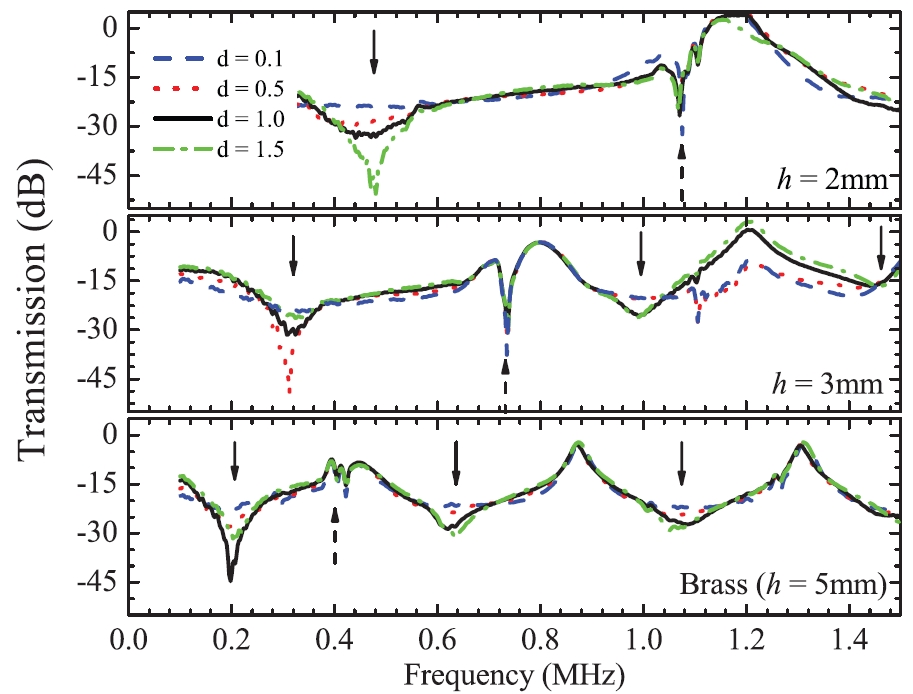
\includegraphics[width = 0.85\linewidth]{experimentRayleigh.jpg}
\caption{Experimental sound transmission spectra of a~water slit between two brass plates for different channel width $d$ and length $h$, reported in \cite{channel1}. The~vertical arrows indicate the~frequencies at which the~transmission is extraordinarily low. \textit{Image reprinted from \cite{channel1}, CC BY 3.0.}}
\label{fig:experimentRayleigh}
\end{center}
\end{figure}

Intuitively, the~reason for the~emergence of the~unexpected minima in \cref{fig:experimentRayleigh} has to be the~destructive interference of waves that propagate in the~channel --- the~same reason that explains the~Fabry-Perot resonances.
Of course, the~interfering waves must now be the~proper eigenmodes of the~system, that is, of the channel between the plates.
Further, I will present the~theory of sound transmission through a~slit formed by two solid plates, taking into account the~elastic nature of the~latter.
The~eigenmodes of the~system in question are essentially the~Rayleigh waves modified by coupling to the~fluid environment.
This modification makes the~eigenmodes lose their orthogonality with respect to each other.
Having a~nonorthogonal basis of eigenfunctions is quite typical for problems involving elastic solids, e.g., it is known that the~elastic modes of an~isolated solid plate (the~Rayleigh-Lamb modes) are not orthogonal as well \cite{achenbac}.
Moreover, the~channel eigenmodes belong to two main categories: the~true surface, or propagating, modes, and the~leaky modes, though the~nonorthogonality makes explicit separation of modes impossible.
The~latter observation applies also to electromagnetic domain, see, for example, discussion in \cite{sturman2} regarding the~metal-dielectric waveguides.

The~analytical solution to the~scattering problem relies on the~expansion of the~acoustic fields in series over both types of those coupled Rayleigh modes propagating in the~channel.
I also generalize the~approach to account for the~nonorthogonality of the~eigenmodes.
Ultimately, I will demonstrate how the~fluid channel that partially transmits sound via the~leaky waves effectively serves as a~redirecting acoustic antenna, and that the~effect of redirection of sound causes the~suppression of both transmission and reflection.
In the~rigid-body approximation, producing such an~effect is clearly infeasible.
For that reason, this effect should not be confused with other previously mentioned manifestations of the~strong suppression of sound \cite{norris4,estrada,estrada2,estrada3}, which introduce Fano-like resonances into the~transmission spectrum even in the~rigid-body approximation.
%The~complete basis of coupled Rayleigh eigenmodes will be used to expand the~acoustic fields in the~channel and the~plates in series.



%Here we develop a~theory of sound transmission through a~slit formed by two elastic solid plates. We solve the~eigenvalue problem for the~whole system which consists of two elastic infinite plates coupled through a~straight fluid channel. The~acoustic field is expanded over the~set of eigenfunctions which describe synchronized vibrations of the~whole system. Each eigenfunction is characterized by complex eigenvector, i.e. these eigenfunctions are {\it inhomogeneous} plane waves. Lack of orthogonality presents certain mathematical difficulties in calculations. Nevertheless, the~expansion over this nonorthogonal basis converges sufficiently fast, providing very good agreement with experimental results in the~whole frequency range.  Using the~proposed theory we show that at the~frequencies when the~deep minima in transmission are observed the~reflection  is also minimal.
%This occurs due to formation of quasi-standing Rayleigh wave in the~whole system.
%Since the~transmission and reflection are strongly suppressed, the~only way for the~accumulated elastic energy to escape is radiation into metal. 

%The~rate of radiation into metal is relatively  high, i.e. a~straight fluid channel serves as redirecting acoustic antenna. The~proposed mechanism is very different from the~ strong suppression of sound transmission through a~periodic arrangements of holes in a~rigid screen \cite{norris4,estrada,estrada2}. The~latter is due to destructive interference between the~Fabry-Perot cavity mode and the~Fourier component of the~acoustic field in the~fluid with the~wavelength equal to the~period of perforation.  This Fano-like resonance exists even in the~rigid-body approximation and is manifested as total reflection of sound wave from the~perforated solid plate. Unlike this, the~proposed effect of redirection of sound leads to suppression of both, transmission and reflection, and it vanishes in the~rigid-body approximation.


%%%%%%%%%%%%%%%%%%%%%%%%%%%%%%%%%%%%%%%%%%%%%%%%%%%%%%%%%%%%%%%%%%%%
\section{Acoustic Potentials}

\subsection{Scalar Potential for Pressure Waves in Fluids}

In this chapter, I neglect the~effects of viscosity and treat the~propagation of sound as a~laminar (nonturbulent) process in the~fluid which is otherwise stationary.
With that, only longitudinal pressure waves can exist within the~volume of the~fluid, and the~resulting pressure oscillations are known to be adiabatic, meaning that the~wave does not lose or gain energy from the~background.

The~complete description of the~fluid dynamics requires knowledge of either the~local velocity $\mathbf{v}_f(\mathbf{r}, t)$ or both the local pressure $p_f(\mathbf{r}, t)$ and density $\rho_f(\mathbf{r}, t)$ at any given position $\mathbf{r}$ and moment of time $t$.
These quantities are related since one must satisfy both the~continuity equation
\begin{equation}
\label{eq:continuityRayleigh}
\frac{\partial\rho_f}{\partial t} + \nabla\cdot\left(\rho_f\mathbf{v}_f\right) = 0,
\end{equation}
which guarantees the~conservation of mass in the~system, and the~momentum equation
\begin{equation}
\label{eq:secondNLRayleigh}
\frac{\partial \rho_f\mathbf{v}_f}{\partial t} + \nabla p_f = 0,
\end{equation}
which is essentially the~Newton's second law applied to a~unit volume of fluid.

Assuming the~propagating wave is only a~small perturbation of the~fluid stationary state, the~dynamic properties of the~fluid are linearized as
\begin{align}
p_f(\mathbf{r}, t)~&=~p_0 + p(\mathbf{r}, t), \label{eq:pressureLinearRayleigh}\\
\rho_f(\mathbf{r}, t)~&=~\rho_0 + \rho(\mathbf{r}, t), \label{eq:densityLinearRayleigh}\\
\mathbf{v}_f(\mathbf{r}, t)~&=~\mathbf{v}_0 + \mathbf{v}(\mathbf{r}, t), \label{eq:velocityLinearRayleigh}
\end{align}
where $p_0$, $\rho_0$, and $\mathbf{v}_0$ describe the~background acoustic field, and the~smallness of perturbations can be understood, for example, as $|p(\mathbf{r}, t)| \ll p_0$.
The~assumption of no background flow gives $\mathbf{v}_0=0$, and the~absence of the vortices yields $\nabla\times\mathbf{v}(\mathbf{r}, t)=0$.

The~longitudinal sound wave propagates with a~constant phase speed, which is given by
\begin{equation}
c_f = \sqrt{\left(\frac{\partial p_f}{\partial \rho_f}\right)_s},
\end{equation}
where the~derivative is calculated for an~adiabatic process, i.e., at constant entropy.
Using \cref{eq:pressureLinearRayleigh}-\cref{eq:densityLinearRayleigh}, one can relate the~local variations of pressure and density as
\begin{equation}
p(\mathbf{r}, t) = \rho(\mathbf{r}, t)c_f^2.
\end{equation}

Consequently, the~wave equation for the~pressure $p(\mathbf{r},t)$,
\begin{equation}
\label{eq:waveeqPRayleigh}
\Delta p - \frac{1}{c_f^2}\frac{\partial^2 p}{\partial t^2}~=~0,
\end{equation}
is immediately obtained after one substitutes \cref{eq:secondNLRayleigh} into \cref{eq:continuityRayleigh} and uses the~linearizations \cref{eq:pressureLinearRayleigh}-\cref{eq:velocityLinearRayleigh} while discarding the~terms that are quadratic over small perturbation.
%
The~condition $\nabla\times\mathbf{v}(\mathbf{r}, t) = 0$ allows to represent the~velocity as a~gradient of a~scalar function (fluid is then said to be in a state of a potential flow):
\begin{equation}
\mathbf{v}(\mathbf{r}, t)=\nabla B(\mathbf{r}, t).
\end{equation}
For monochromatic waves with the~time dependence given by $e^{-i\omega t}$ factor, the~equation \cref{eq:secondNLRayleigh} relates the~velocity to the~gradient of pressure
\begin{equation}
\label{eq:vandpRayleigh}
i\omega\rho_0\mathbf{v}(\mathbf{r},t) = \nabla p(\mathbf{r},t),
\end{equation}
and, therefore, one may define the~acoustic potential $B(\mathbf{r}, t)$ as
\begin{equation}
\label{eq:potentialBRayleigh}
B(\mathbf{r}, t) = \frac{p(\mathbf{r},t)}{i\omega\rho_0}.
\end{equation}
From \cref{eq:waveeqPRayleigh}-\cref{eq:potentialBRayleigh} it is obvious that the~potential $B(\mathbf{r}, t)$ satisfies the~wave equation
\begin{equation}
\label{eq:waveeqBRayleigh}
\Delta B - \frac{1}{c_f^2}\frac{\partial^2 B}{\partial t^2}~=~0,
\end{equation}
and that it uniquely defines the~local pressure and velocity of the~fluid.

Since the~density variations are small, the~approximate equality $\rho_f(\mathbf{r}, t) \approx \rho_0$ holds, and in the~sections below I will not distinguish between these two quantities and will use the~notation $\rho_f$ instead of $\rho_0$.


\subsection{Scalar and Vector Potentials for Elastic Waves in Solids}

Unlike fluids which take the~shape of the~volume they occupy, the~elastic properties of solids allow them to resist the~changes to their shape in order to reestablish their original form and size.
As a~result, two distinct types of waves can propagate in the~bulk of a~solid --- longitudinal (compressional) and transverse (shear).
In these waves, the~particle oscillations occur either along or perpendicular to the~direction of wave propagation, respectively.
The~local displacement field $\mathbf{u}(\mathbf{r},t)$ and stress tensor $\sigma_{ik}(\mathbf{r}, t)$ are typically used to describe the~dynamics of a~solid.
The~Newton's second law applied to a~unit volume of the~solid
\begin{equation}
\rho_m\frac{\partial u_i}{\partial t} = \frac{\partial \sigma_{ik}}{\partial x_k},
\end{equation}
where the~Einstein summation convention for tensors is implied, ultimately leads to the~following general wave equation for elastic waves \cite{LLtom7}:
\begin{equation}
\label{eq:waveeqURayleigh}
\frac{\partial^2 \mathbf{u}}{\partial t^2}~=~c_t^2 \Delta\mathbf{u} + \left(c_l^2-c_t^2\right)\nabla\left(\nabla\cdot\mathbf{u}\right).
\end{equation}
Here $\rho_m$ is the~density of the~solid and $c_l$($c_t$) is the~speed of the~pure longitudinal (transverse) acoustic wave.
The~two speeds of sound are expressed through the~so-called Lam\'e parameters of the~solid, $\lambda$ and $\mu$:
\begin{equation}
c_l~=~\sqrt{\frac{\lambda+2\mu}{\rho}}, \qquad c_t~=~\sqrt{\frac{\mu}{\rho}},
\end{equation}
which in their turn represent the~bulk and shear moduli $K$ and $G$:
\begin{equation}
K~=~\lambda+\frac23\,\mu, \qquad G~=~\mu.
\end{equation}

Since, according to the~Helmholtz decomposition theorem, the~vector quantity $\mathbf{u}(\mathbf{r},t)$ can always be represented as a~sum of a~potential and a~solenoidal field:
\begin{equation}
\mathbf{u} = \mathbf{u}_l + \mathbf{u}_t,
\end{equation}
where $\nabla\times\mathbf{u}_l = 0$ and $\nabla\cdot\mathbf{u}_t = 0$, it allows splitting \cref{eq:waveeqURayleigh} into two independent wave equations
\begin{equation}
\label{eq:waveeqUltRayleigh}
\Delta\mathbf{u}_{l,t} - \frac{1}{c_{l,t}^2}\frac{\partial^2 \mathbf{u}_{l,t}}{\partial t^2}~=~0
\end{equation}
for both longitudinal and transverse components of the~elastic wave and introduce the~scalar potential $L(\mathbf{r}, t)$ and the~vector potential $\mathbf{S}(\mathbf{r}, t)$ as
\begin{equation}
\mathbf{u}_l(\mathbf{r}, t)~=~\nabla L(\mathbf{r}, t), \qquad \mathbf{u}_t(\mathbf{r}, t)~=~\nabla\times\mathbf{S}(\mathbf{r}, t).
\end{equation}

With the~scalar potential $L$ corresponding to the~pressure wave and the~vector potential $\mathbf{S}$ representing the~shear wave, naturally, they satisfy the~respective wave equations:
\begin{align}
\Delta L - \frac{1}{c_l^2}\frac{\partial^2 L}{\partial t^2}~&=~0, \label{eq:waveeqLRayleigh}\\
\Delta \mathbf{S} - \frac{1}{c_t^2}\frac{\partial^2 \mathbf{S}}{\partial t^2}~&=~0, \label{eq:waveeqSRayleigh}
\end{align}
and uniquely define the~local displacement of the~solid
\begin{equation}
\label{eq:displacementRayleigh}
\mathbf{u}(\mathbf{r}, t)~=~\nabla L(\mathbf{r}, t) + \nabla\times\mathbf{S}(\mathbf{r}, t)
\end{equation}
and stress tensor (through Hooke's law)
\begin{equation}
\label{eq:HookesLawRayleigh}
\sigma_{ik}(\mathbf{r}, t)~=~\lambda u_{ll}(\mathbf{r}, t)\delta_{ik} + 2\mu u_{ik}(\mathbf{r}, t).
\end{equation}
Here $u_{ik}$ denotes the~strain tensor $u_{ik}=\frac12\left(\frac{\partial u_i}{\partial x_k}+\frac{\partial u_k}{\partial x_i}\right)$, and $\delta_{ik}$ is the~Kronecker delta.

Note that the~potentials themselves are not defined uniquely, specifically, adding a~curl of an~arbitrary vector function to $L(\mathbf{r}, t)$ or adding a~gradient of an~arbitrary scalar function to $\mathbf{S}(\mathbf{r}, t)$ does not change the~displacement field $\mathbf{u}(\mathbf{r}, t)$.


\subsection{Fluid-Solid Boundary Conditions}

When a~fluid and a~solid occupy adjacent regions of space, the~boundary conditions must be specified at the~fluid-solid interface (see \cite{lloyd}, for example).
The~continuity of the~normal component of the~local velocity
\begin{equation}
\label{eq:boundaryVelocityRayleigh}
\left.v_n\right|_\Sigma~=~\left.\dot{u}_n\right|_\Sigma
\end{equation}
ensures that the~two media neither permeate each other nor produce void regions between them along the~interface $\Sigma$.
As the~fluid is nonviscous, there is no binding between the~tangential components of velocities, and the~particles of the~fluid do not stick to the~surface of the~solid.

Other than that, the~balance between the~stress of the solid and the~pressure in the~fluid
\begin{equation}
\label{eq:boundaryStressRayleigh}
\left.\sigma_{ik}n_k\right|_\Sigma = - \left.p n_i\right|_\Sigma
\end{equation}
must be enforced.
Here the~vector $n_i$ is the~external normal to the~surface $\Sigma$, and due to the~absence of shear interactions in fluid its pressure is acting perpendicular to $\Sigma$: $p_i = -p n_i$.



%%%%%%%%%%%%%%%%%%%%%%%%%%%%%%%%%%%%%%%%%%%%%%%%%%%%%%%%%%%%%%%%%%%%
\section{Rayleigh Waves on the~Surface of a~Solid}

When considering the~propagation of elastic waves in the~bulk of a~solid, one infers the~independence of pressure waves from shear waves in the~sense that the~wave amplitudes are not tied to each other.
However, a~specific relationship between the~amplitudes arises when the~waves propagate close to the~surface of the~solid, which requires satisfying the~boundary conditions \cref{eq:boundaryVelocityRayleigh}-\cref{eq:boundaryStressRayleigh}.
In particular, the~wave equation \cref{eq:waveeqURayleigh} was shown to have a~surface wave solution --- the~so-called Rayleigh wave \cite{rayleigh}, which intertwines both longitudinal and transverse particle motion and is concentrated in the~vicinity of the~surface, exponentially vanishing away from it.
The~Rayleigh waves are typically distinguished from the~Lamb waves, which are the~elastic surface waves as well, but are specific for the~thin solid plates.

%\subsection{Solid-Vacuum Interface}

The~concept of Rayleigh waves is normally demonstrated in the~simplified situation, where the~solid borders with the~vacuum \cite{LLtom7}.
Here I assume the~planar interface that coincides with the~plane $z=0$ (where the~region $z>0$ is occupied by solid), and I seek the~monochromatic solution to \cref{eq:waveeqLRayleigh}-\cref{eq:waveeqSRayleigh} which propagates in the~$x$-direction and exponentially decays with $z$.
This solution is only valid in the~region $z\ge 0$, as in the~vacuum the~sound does not propagate.

The~independent of the~coordinate $y$ acoustic potentials can thus be written down as
\begin{align}
L(x,z,t)~&=~l\,e^{i\beta x-\nu z-i\omega t}, \qquad z \ge 0, \\
\mathbf{S}(x,z,t)~&=~\mathbf{s}\,e^{i\beta x-\eta z-i\omega t}, \qquad z \ge 0,
\end{align}
where $\beta$ is the~$x$-component of the~wavevector, $l$ and $\mathbf{s} = (s_x, s_y, s_z)$ are the~amplitudes of the~potentials.
The~quantities $\nu$ and $\eta$ are defined as
\begin{align}
\nu~&=~\sqrt{\beta^2-k_l^2}, &\beta \ge k_l=\frac{\omega}{c_l}, \label{eq:nuRayleigh}\\
\eta~&=~\sqrt{\beta^2-k_t^2}, &\beta \ge k_t=\frac{\omega}{c_t}. \label{eq:etaRayleigh}
\end{align}
%
The~components of the~displacement field are calculated from the~potentials using \cref{eq:displacementRayleigh}:
\begin{align}
u_x~&=~\frac{\partial L}{\partial x} - \frac{\partial S_y}{\partial z}~=~\left(i\beta e^{-\nu z}\cdot l+\eta e^{-\eta z}\cdot s_y\right)e^{i\beta x-i\omega t}, \label{eq:uxRayleigh}\\
u_y~&=~\frac{\partial S_x}{\partial z} - \frac{\partial S_z}{\partial x}~=~-\left(\eta\cdot s_x+i\beta \cdot s_z\right)e^{-\eta z}e^{i\beta x-i\omega t}, \label{eq:uyRayleigh}\\
u_z~&=~\frac{\partial L}{\partial z} + \frac{\partial S_y}{\partial x}~=~\left(-\nu e^{-\nu z}\cdot l+i\beta e^{-\eta z}\cdot s_y\right)e^{i\beta x-i\omega t}. \label{eq:uzRayleigh}
\end{align}

The~solid-vacuum boundary is a~free boundary, so one may only demand that any infinitesimal part of the~interface is stress-free, namely, that
\begin{equation}
\sigma_{xz}~=~\sigma_{yz}~=~\sigma_{zz}~=~0,
\end{equation}
at the~interface $z=0$, or, more explicitly,
\begin{equation}
\label{eq:sigmaxzyzzzRayleigh}
\left\{\begin{array}{rll}
0~=~\sigma_{xz}~&=~2\mu u_{xz}~&=~\mu \left(\dfrac{\partial u_x}{\partial z}+\dfrac{\partial u_z}{\partial x}\right), \\
0~=~\sigma_{yz}~&=~2\mu u_{yz}~&=~\mu \dfrac{\partial u_y}{\partial z}, \\
0~=~\sigma_{zz}~&=~2\mu u_{zz}+\lambda \nabla\cdot\mathbf{u}~&=~2\mu \dfrac{\partial u_z}{\partial z} + \lambda\left(\dfrac{\partial u_x}{\partial x}+\dfrac{\partial u_z}{\partial z}\right).
\end{array}\right.
\end{equation}

The~second equation in the~system suggests that $u_y = 0$, and without any loss of generality one may equate both $s_x$ and $s_z$ to zero, thus leaving $s_y$ as the~only nonzero component of the~coefficient $\mathbf{s}$.
This becomes possible due to the~fact that one may add a~gradient of any scalar function to $\mathbf{S}(\mathbf{r}, t)$ without any effect on the~displacement field.
If one now selects this scalar function to be $f(\mathbf{r}, t) = \left(s_z/\eta\right) e^{i\beta x-\eta z-\i\omega t}$, then the~redefined potential $\mathbf{S}'(\mathbf{r}, t) = \mathbf{S}(\mathbf{r}, t) + \nabla f(\mathbf{r}, t)$ will automatically have $S'_z = 0$, and it will also have $S'_x = 0$ due to the~relation \cref{eq:uyRayleigh} and the~condition $u_y=0$.
With this, I will further assume the~vector potential to have only nonzero $y$-component, $\mathbf{S}(\mathbf{r}, t) = \left(0, S(\mathbf{r}, t), 0\right)$, and $\mathbf{s}=\left(0,s,0\right)$.
It is worth mentioning that even though the~wave is propagating along the~$x$-axis, its amplitude, nevertheless, varies with the~coordinate $z$, causing the~vector potential to give a~nonzero contribution to the~displacement $u_x$, and it is thus impossible to break down the~Rayleigh wave into independent longitudinal and transverse components.

Now, using \cref{eq:uxRayleigh}-\cref{eq:uzRayleigh}, the~first and the~third equations from \cref{eq:sigmaxzyzzzRayleigh} are reduced to
\begin{equation}
\left\{\begin{array}{rrrr}
\left(\beta^2+\eta^2\right)\cdot s &+&2i\beta\nu\cdot l~&=~0, \\
-2i\mu\beta\eta\cdot s &+& \left(2\mu\nu^2-\lambda k_l^2\right)\cdot l~&=~0, \\
\end{array}\right.
\end{equation}
The~obtained system has a~nontrivial solution if and only if its determinant equals zero, namely, if
\begin{equation}
\frac{1}{\mu}\left(2\mu\nu^2-\lambda k_l^2\right)\left(\beta^2+\eta^2\right)-4\beta^2\eta\nu~=~0,
\end{equation}
or, when simplified,
\begin{equation}
\left(\eta^2+\beta^2\right)^2-4\nu\eta\beta^2~=~0.
\end{equation}

The~latter expression implicitly relates the~frequency of the~wave $\omega$ and its wavevector $\beta$, and it can be rewritten for the~dimensionless phase velocity $\xi=\omega/\beta c_t$ as
\begin{equation}
\label{eq:dispNoRHSRayleigh}
\left(2-\xi^2\right)^2-4\sqrt{1-\xi^2}\sqrt{1-\frac{c_t^2}{c_l^2}\xi^2}~=~0.
\end{equation}
Since typically $c_t < c_l$ in solids, the~equation \cref{eq:dispNoRHSRayleigh} has only one real root for any value of $c_t/c_l$ which lies in the~range $0 < \xi < 1$; for most common solids, the~dimensionless phase speed is restricted to the~range $0.874 \le \xi \le 0.955$ \cite{LLtom7}.
Such values of $\xi$ describe surface waves which propagate slower than either the~pure pressure or shear wave in the~bulk of the~solid.
For any given solid, the~speed of the~Rayleigh wave is uniquely defined by the~ratio of its transverse and longitudinal speeds of sound, and does not depend on the~wave frequency.

%\subsection{Solid-Fluid Interface}


%%%%%%%%%%%%%%%%%%%%%%%%%%%%%%%%%%%%%%%%%%%%%%%%%%%%%%%%%%%%%%%%%%%%
\section{Coupled Rayleigh Waves in the~Fluid Channel between Two Solid Plates}

\begin{figure}
\begin{center}
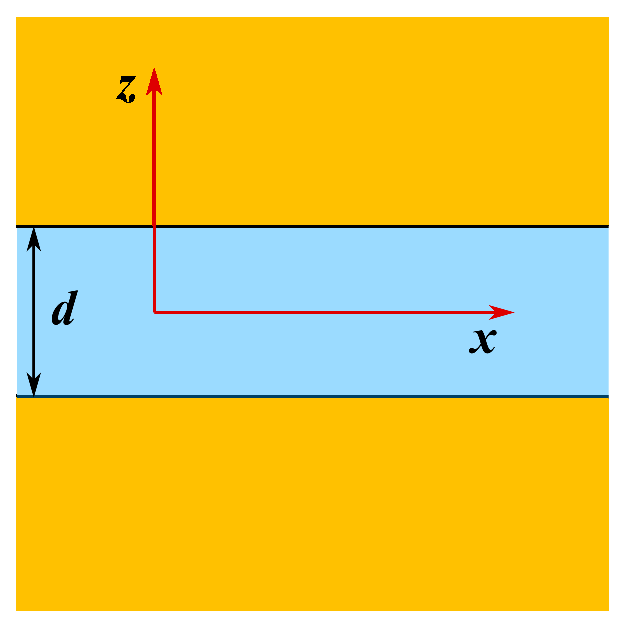
\includegraphics[width=0.5\linewidth]{infinite.eps}
\caption{An~infinite fluid channel between two elastic plates.}
\label{fig:infinite}
\end{center}
\end{figure}

Now I consider a~monochromatic sound wave propagating along an~infinite straight fluid channel of the~width $d$ between two elastic plates (see \cref{fig:infinite}).
The~elastic plates are made from the~same material and they are occupying the~regions $|z| > d/2$.
The~wave is propagating in the~positive $x$-direction.
The~mirror symmetry with respect to the~$xOy$ plane suggests that the~eigenmodes of the~system are either even or odd functions of the~coordinate $z$.
More precisely, I will be using the~term "even" to describe the~eigenmodes with $u_x$ being an~even and $u_z$ being an~odd function of $z$.
The~term "odd" will then refer to any mode with $u_x$ being an~odd function of $z$.
In terms of potentials, the~even mode corresponds to all potentials being even functions of $z$.

Below, I will analyze only the~even modes and pay no attention to the~odd modes.
The~reason for that is the~mirror symmetry with respect to the~$x$-axis that will be enforced everywhere in the~subsequent sections.
For the~scattering problem it means that the~impinging wave should be incident only normally at the~system, along the~$x$-axis.
The~excitation of the~odd modes will not be possible at all as they violate the~symmetry.
However, the~odd modes can be excited if the~problem loses its symmetry with respect to $xOy$ plane, either by allowing the~oblique incidence of the~sound wave or by having the~elastic plates made from different materials \cite{channel1}.

\subsection{Dispersion Relation}

The~symmetric solution of the~wave equations \cref{eq:waveeqBRayleigh}, \cref{eq:waveeqLRayleigh}, and \cref{eq:waveeqSRayleigh} is as follows (the~factor $e^{-i\omega t}$ is omitted everywhere below):
\begin{align}
B(x,z)~&=~b\,e^{i\beta x}\cos{kz}, &|z| < d/2, \label{eq:potBcoupledRayleigh}\\
L(x,z)~&=~l\,e^{i\beta x-\nu|z|}, &|z| > d/2, \label{eq:potLcoupledRayleigh}\\
S_y(x,z)~&=~s\,e^{i\beta x-\eta|z|}, \qquad S_x=S_z=0, &|z| > d/2, \label{eq:potScoupledRayleigh}
\end{align}
where $k=\sqrt{k_f^2-\beta^2}$, $k_f=\omega/c_f$.
Both $\nu$ and $\beta$ are defined as earlier in \cref{eq:nuRayleigh}-\cref{eq:etaRayleigh} except that no restriction is placed on the~value of $\beta$.

Because of the~symmetry, it is sufficient to write the~boundary conditions only for, e.g. $z=d/2$.
At this fluid-metal interface the~stress and the~normal component of the~velocity are continuous:
\begin{equation}
\sigma_{zz}~=~-p, \qquad \sigma_{xz}~=~0, \qquad \dot{u}_z~=~v_z,
\end{equation}
as follows from \cref{eq:boundaryVelocityRayleigh}-\cref{eq:boundaryStressRayleigh}.
The~stress tensor component $\sigma_{yz}$ is identically zero due to the~choice of the~vector potential $\mathbf{S}$.

Similarly to the~derivations in the~previous section, the~boundary conditions yield the~following system where all the~potentials are evaluated at $z=d/2$:
\begin{equation}
\left\{\begin{aligned}
-\lambda k_l^2 L +2\mu\left(\frac{\partial^2 L}{\partial z^2}+\frac{\partial^2 S}{\partial x \partial z}\right)~&=~-i\omega\rho_f B, \\
\mu\left(2\frac{\partial^2 L}{\partial x \partial z}+\frac{\partial^2 S}{\partial x^2}-\frac{\partial^2 S}{\partial z^2}\right)~&=~0, \\
-i\omega\left(\frac{\partial L}{\partial z} + \frac{\partial S_y}{\partial x}\right)~&=~\frac{\partial B}{\partial z},
\end{aligned}\right.
\end{equation}
which is reduced to
\begin{equation}
\label{eq:coeffRelationsRayleigh}
\left\{
\begin{array}{rrrrrr}
\left(2\mu\nu^2-\lambda k_l^2\right)\,e^{-\nu d/2}\cdot l &-& 2i\mu \eta \beta\,e^{-\eta d/2}\cdot s &+& i\omega\rho_f \cos(k d/2)\cdot b~&=~0, \\
2i\nu \beta \,e^{-\nu d/2}\cdot l &+& \left(\beta^2 +\eta^2 \right)e^{-\eta d/2} \cdot s &&~&=~0, \\
i\omega\nu \,e^{-\nu d/2}\cdot l &+& \omega\beta \,e^{-\eta d/2}\cdot s &+& k \sin(k d/2)\cdot b~&=~0. \\
\end{array}
\right.
\end{equation}
This set of homogeneous linear equations has a~nontrivial solution if its determinant vanishes, which is expressed by the~condition
\begin{equation}
\label{eq:dispersionkRayleigh}
\left(\eta^2+\beta^2\right)^2-4\nu\eta\beta^2~=~\frac{\rho_f}{\rho_m}\frac{\omega^4}{c_t^4}\frac{\nu}{k}\,\cot \frac{kd}{2}.
\end{equation}
Since all the~quantities $k$, $\nu$, and $\eta$ are expressed through $\omega$ and $\beta$, the~latter equation is essentially the~dispersion relation for the~coupled Rayleigh waves propagating in the~fluid channel.
This relation can be rewritten in terms of the~dimensionless frequency $\Omega = \omega d/c_t$ and wavevector $q = \beta d$, which allows to eliminate the~dependence on the~channel width $d$ from the~picture:
\begin{equation}
\label{eq:dispersionqRayleigh}
\left(2 q^2-\Omega^2\right)^2 - 4 q^2 \sqrt{q^2 - (c_t/c_l)^2 \Omega^2} \sqrt{q^2 - \Omega^2} 
~=~ \frac{\rho_f}{\rho_m}\Omega^4 \sqrt{\frac{q^2 - (c_t/c_l)^2 \Omega^2}{(c_t/c_f)^2 \Omega^2 - q^2}}\,\cot\left( \frac{1}{2}\sqrt{\frac{c_t^2}{c_f^2} \Omega^2 - q^2}\right).
\end{equation}
Also, the~dispersion relation for the~dimensionless phase velocity $\xi=\omega/\beta c_t$ can be obtained from the~latter by substituting $q=\Omega /\xi$:
\begin{equation}
\label{eq:dispersionXiRayleigh}
\left(2-\xi^2\right)^2-4\sqrt{1-\xi^2}\sqrt{1-\frac{c_t^2}{c_l^2}\xi^2}
~=~\frac{\rho_f}{\rho_m}\,\xi^4 \sqrt{\frac{1-\left(c_t/c_l\right)^2\xi^2}{\left(c_t/c_f\right)^2\xi^2-1}}\cot\!\left(\frac{\Omega}{2\xi}\sqrt{\frac{c_t^2}{c_f^2} \xi^2-1}\,\right).
\end{equation}
Real and complex solutions of the~dispersion relation \cref{eq:dispersionqRayleigh} define the~allowed values of the~wave vector $q = q(\Omega)$ for each frequency $\Omega$, and \cref{eq:dispersionXiRayleigh} gives the~allowed phase velocities $\xi = \xi(\Omega)$.


\subsection{Analysis of the~Dispersion Branches}

For any frequency $\Omega$, the~dispersion equation \cref{eq:dispersionXiRayleigh} has a~finite number of real ($\xi = \re \xi > 0$) and an~infinite number of complex ($\re \xi > 0$, $\im \xi < 0$) roots.
The~condition $\re\xi>0$ ensures that the~eigenmodes found indeed propagate forward in the~$+x$-direction.
Since the~phase speed $\xi$ enters \cref{eq:dispersionXiRayleigh} only as $\xi^2$, it is obvious that a~negative of any root $\xi$ with a~positive real part also satisfies the~dispersion equation.
Such roots describe the~backward propagating Rayleigh waves, i.e., in the~$-x$-direction.

In the~numerical analysis below, I will be using the~parameters of water ($\rho_f=1000$ kg/m$^3$, $c_f=1500$ m/s) and brass ($\rho_m=8400$ kg/m$^3$, $c_t=2000$ m/s, $c_l=4250$ m/s).

\subsection{Real Eigenmodes}

The~eigenmodes with real $\xi$ have real wavevector $q$, and, therefore, they are propagating modes.
If the~losses in the~media are neglected, these true modes will never decay as they propagate along the~channel.
Due to the~term $\sqrt{1-\xi^2}$ in \cref{eq:dispersionXiRayleigh}, the~value of $\xi$ must be restricted to the~range $0 < \xi \le 1$.
This means that in \cref{eq:potBcoupledRayleigh}-\cref{eq:potScoupledRayleigh} the~values of $\beta$, $\nu$, and $\eta$ are purely real which provides the~oscillating behavior along the~channel and the~decay of the~acoustic field into the~solid away from the~channel.
As for the~value of $k$, it may be either purely real (when $c_f/c_t < \xi \le 1$) or purely imaginary (when $0 < \xi < c_f/c_t$).
Here I assume that $c_f < c_{l,t}$, since the~speed of sound in fluids is considerably lower than the~speed of sound in solids.
%
In the~first case, the~acoustic potential in the~fluid oscillates along $z$ as well and the~sound wave has a~wavefront of constant amplitude inside the~channel.
The~two Rayleigh waves on each fluid-solid interface are strongly coupled as the~sound energy is not concentrated in the~vicinity of either interface but rather confined to the~whole width of the~channel.
In the~second case, the~potential \cref{eq:potBcoupledRayleigh} becomes $B(x,z)=b\,e^{ibx}\cos{kz}=b\,e^{ibx}\cosh{|kz|}$, so that the~sound energy both in the~solid and in the~fluid is mostly concentrated near the~interfaces. 

These two types of true eigenmodes will further be referred to as fast and slow modes since the~former propagate faster than the~speed of sound in fluid, and the~latter propagate slower, respectively.

The~dispersion equation \cref{eq:dispersionXiRayleigh} is transcendental and can only be solved numerically.
Nevertheless, a~certain asymptotic analysis of the~eigenmode dispersion is still possible.
I start by considering the~fast modes.
I note that the~left-hand side of \cref{eq:dispersionXiRayleigh} is clearly identical to that of \cref{eq:dispNoRHSRayleigh}.
Its right-hand side thus describes the~coupling of two individual Rayleigh waves on each interface through the~fluid.
The~coupling strength is proportional to the~ratio $\rho_f/\rho_m$. 
In the~absence of the~fluid, $\rho_f=0$, the~coupling term disappears and the~surface waves in each plate become uncoupled.
These surface waves are the~same Rayleigh waves described by \cref{eq:dispNoRHSRayleigh}, with their phase speed $\xi=\xi_R$ independent from the~frequency.
Thus in the~limit $\rho_f/\rho_m \ll 1$, when the~right-hand side of \cref{eq:dispersionXiRayleigh} is small, the~coupled Rayleigh waves should be almost dispersionless.

However, the~previous argument cannot be valid if the~argument of the~cotangent $kd/2$ is close to an~integer of $\pi$, in which case the~value of the~cotangent outmatches the~smallness of $\rho_f/\rho_m$.
The~condition $kd/2\pi=0,1,2,...$ corresponds to the~potential \cref{eq:potBcoupledRayleigh} being a~standing wave with its velocity nodes at the~channel walls, which can be seen by calculating $v_z$:
\begin{equation}
\left.v_z(x,z)\right|_{z=\frac{d}{2}}~=~\left.\frac{\partial B}{\partial z}\right|_{z=\frac{d}{2}}~=~-kb e^{i\beta x}\sin{\frac{kd}{2}}~=~0.
\end{equation}
In other words, the~coupled Rayleigh wave behaves identically to a~waveguide mode of a~channel with ideally rigid walls.
The~dispersion of the~symmetric waveguide modes consists of an~infinite number of branches
\begin{equation}
\label{eq:waveguideRayleigh}
\omega_n=c_f\sqrt{\left(\frac{2\pi n}{d}\right)^2+\beta^2}, \qquad n=0,1,2,...
\end{equation}
These branches serve as asymptotic boundaries for the~dispersion branches of the~coupled Rayleigh waves.
Each waveguide mode appears after its respective cutoff frequency with the~wavevector $\beta=0$, and features an~infinite phase velocity $\omega_n/\beta$ (except for the~mode $n=0$).

Similar to the~waveguide modes, each individual Rayleigh modes also emerges only after a~corresponding cutoff frequency.
However, the~condition $\beta=0$ does not define the~cutoff frequency in this case since the~phase speed $\xi$ of the~fast modes cannot be infinite: $c_f/c_t < \xi \le 1$.
Clearly, every new dispersion branch must then start with $\xi=1$, which gives the~dimensionless cutoff frequencies
\begin{equation}
\label{eq:cutoffRayleigh}
\Omega_{n} = \frac{\omega_n d}{c_t}= \frac{2}{\sqrt{(c_t/c_f)^2 -1}} \left[ \pi \left(n-1\right) +
\arctan\left(\frac{\rho_f}{\rho_m} \sqrt{\frac{1-(c_t/c_l)^2}{(c_t/c_f)^2-1}}\, \right)\right] ,\,\, n = 1,2, \dots
\end{equation}
and the~corresponding dimensionless wavevectors $q_n = \Omega_n/\xi = \Omega_n$.

Even for the~first fast mode the~cutoff frequency $\Omega_1$ is nonzero, and thus in the~limit of low frequencies no fast modes can be excited to propagate in the~fluid channel.

Unlike the~fast modes, the~single slow coupled Rayleigh mode exists in the~whole frequency range starting from $\Omega=0$ with $\xi=0$ and asymptotically approaching $\xi=c_f/c_t$ when $\Omega \rightarrow \infty$.
The~slow mode is characterized by purely imaginary $k$, and its dispersion equation
\begin{equation}
\label{eq:dispSlowRayleigh}
\left(2-\xi^2\right)^2-4\sqrt{1-\xi^2}\sqrt{1-\frac{c_t^2}{c_l^2}\xi^2}
~=~-\frac{\rho_f}{\rho_m}\,\xi^4 \sqrt{\frac{1-\left(c_t/c_l\right)^2\xi^2}{1-\left(c_t/c_f\right)^2\xi^2}}\coth\!\left(\frac{\Omega}{2\xi}\sqrt{1-\frac{c_t^2}{c_f^2} \xi^2}\,\right)
\end{equation}
is derived using \cref{eq:potBcoupledRayleigh}-\cref{eq:dispersionkRayleigh}, where $k=i|k|$ and $\cos kz$ is replaced with $\cosh |kz|$ in the~expression for the~potential $B(x,z)$.

For $\xi \ll 1$ and $\Omega \ll 1$, I expand the~left-hand side of the~latter dispersion equation in series over $\xi$ and keep the~most significant term only:
\begin{equation}
-2\left(1-\frac{c_t^2}{c_l^2}\right)\xi^2~\approx~-\frac{\rho_f}{\rho_m}\xi^4 \coth \frac{\Omega}{2\xi}.
\end{equation}
Under the~additional assumption $\Omega \ll \xi$ (which is justified by solving the~dispersion equation at low frequencies numerically) the~cotangent $\coth\dfrac{\Omega}{2\xi}$ can be replaced by its approximate value $\dfrac{2\xi}{\Omega}$, and one obtains
\begin{equation}
\xi^3~\approx~\frac{\rho_m}{\rho_f}\left(1-\frac{c_t^2}{c_l^2}\right)\Omega
\end{equation}
or, in terms of the~wavevector $q=\Omega/\xi$,
\begin{equation}
\label{eq:asymptSlowRayleigh}
\Omega~\approx~\sqrt{\frac{\rho_m}{\rho_f}\left(1-\frac{c_t^2}{c_l^2}\right)}\,q^{3/2}.
\end{equation}
It appears that the~slow mode exhibits an~essentially nonlinear dispersion in the~long-wavelength limit, with the~vanishing phase and group velocities for $\Omega=0$.
The~low-frequency waveguide mode \cref{eq:waveguideRayleigh}, however, features purely linear dispersion (for $n=0$).
This means that the~subwavelength propagation of sound through a~fluid channel is drastically different for the~cases of a~real channel with vibrating walls and of an~ideal channel with rigid walls.
The~same is known for the~transmission of electromagnetic waves through a~deeply subwavelength metallic slit, in which case some interesting features arise that do not exist for perfectly conducting screens \cite{seo,xia}.

In the~high-frequency limit the~phase speed of the~slow mode is bound by the~condition $\xi < c_f/c_t$.
More precisely, the~phase speed $\xi$ asymptotically approaches a~specific value $\xi_{a}$: $\xi \rightarrow \xi_{a} < c_f/c_t$.
This limiting phase speed $\xi_a$ satisfies the~equation
\begin{equation}
\left(2-\xi_a^2\right)^2-4\sqrt{1-\xi_a^2}\sqrt{1-\frac{c_t^2}{c_l^2}\xi_a^2}
~=~-\frac{\rho_f}{\rho_m}\,\xi_a^4 \sqrt{\frac{1-\left(c_t/c_l\right)^2\xi_a^2}{1-\left(c_t/c_f\right)^2\xi_a^2}},
\end{equation}
which is obtained from \cref{eq:dispSlowRayleigh} for high frequencies $\Omega$, where the~value of hyperbolic cotangent is approximately $1$ for large arguments.
The~deviation of $\xi_a$ from $c_f/c_t$ is small whenever the~ratio $\rho_f/\rho_m$ is small.
To demonstrate this, I rearrange the~latter equation as
\begin{equation}
\sqrt{c_f/c_t-\xi_a}\sqrt{c_f/c_t+\xi_a}~=~\frac{\rho_f}{\rho_m}\frac{\left(c_f/c_t\right)\xi_a^4 \sqrt{1-\left(c_t/c_l\right)^2\xi_a^2}}{4\sqrt{1-\xi_a^2}\sqrt{1-\left(c_t/c_l\right)^2\xi_a^2}-\left(2-\xi_a^2\right)^2},
\end{equation}
and for $\rho_f/\rho_m \ll 1$ the~value of $\xi_a$ can be replaced by $c_f/c_t$ everywhere except under the~first square root in the~left-hand side.
This yields
\begin{equation}
\label{eq:xiaRayleigh}
\frac{c_f}{c_t}-\xi_a \approx \frac12\left(\frac{\rho_f}{\rho_m}\right)^2 \left(\frac{\left(c_f/c_t\right)^{9/2} \sqrt{1-\left(c_f/c_l\right)^2}}{4\sqrt{1-\left(c_f/c_t\right)^2}\sqrt{1-\left(c_f/c_l\right)^2}-\left(2-\left(c_f/c_t\right)^2\right)^2}\right)^2.
\end{equation}
The~phase speed of the~slow mode then has the~following asymptotic dependence on the~frequency:
\begin{equation}
\left(\xi_a-\xi\right) \sim e^{-\Omega}, \qquad \Omega \rightarrow \infty,
\end{equation}
which originates from the~approximation $\coth \left(\Omega/2\right) \approx 1+2e^{-\Omega}$ for large values of $\Omega$.
The~dispersion of the~slow mode is then almost linear, $\Omega \approx \xi_a q$, and the~mode propagates slightly slower than the~pure pressure wave in the~fluid.


\begin{figure}
\begin{center}
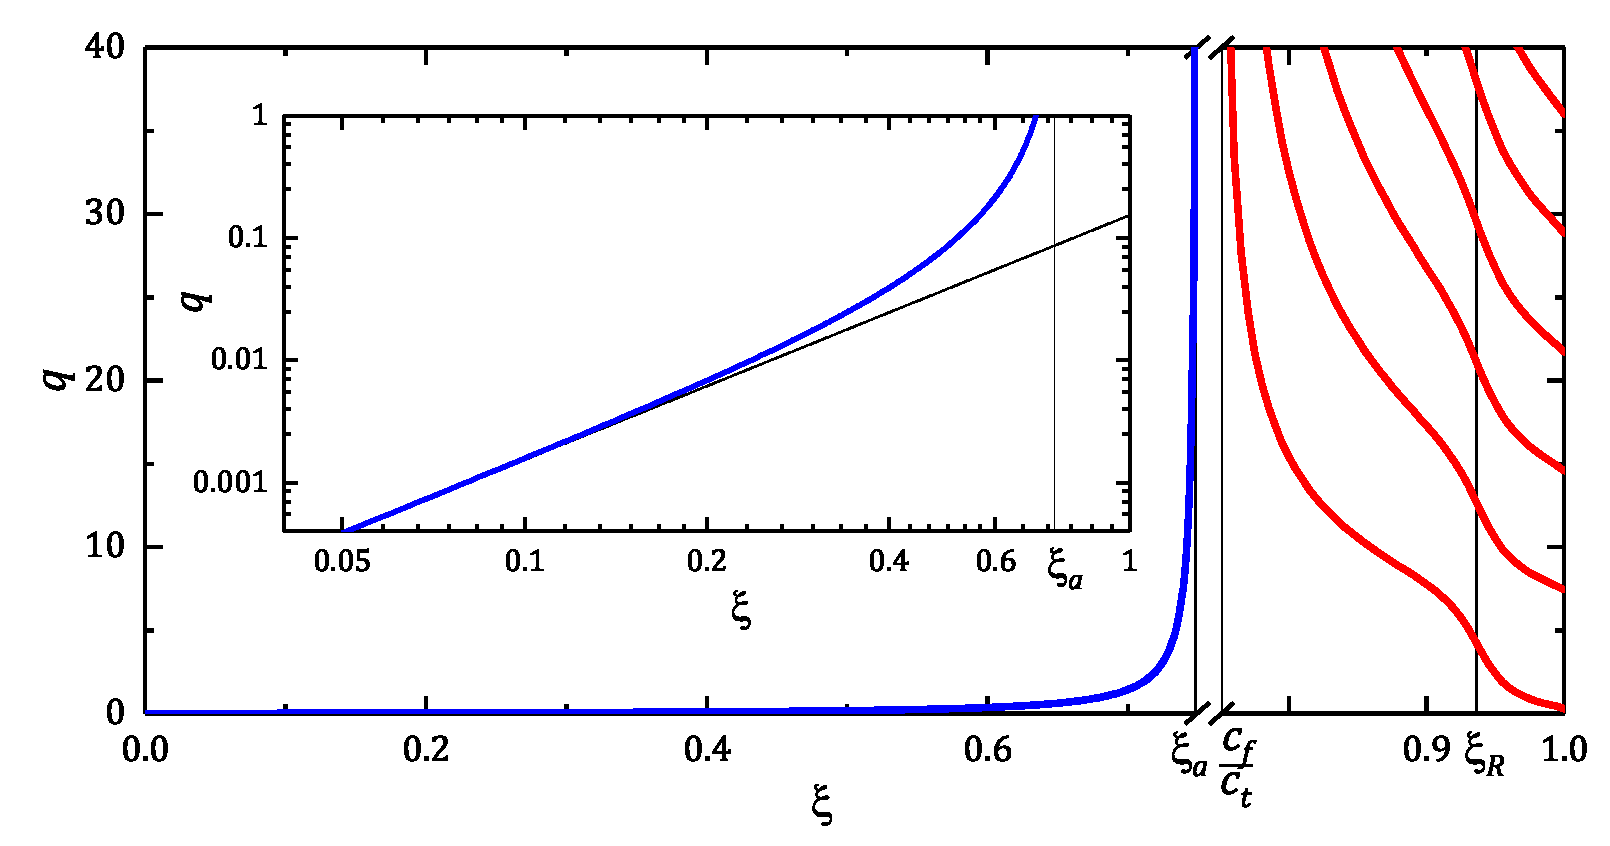
\includegraphics[width=\linewidth]{xi-q.eps}
\caption{Dimensionless phase velocity $\xi=\Omega/q$ vs wave vector $q=\beta d$ for the~infinite water channel between two brass plates, $\rho_f/\rho_m = 0.12$. The~fast mode is represented by an~infinite number of waveguide branches above the~speed of sound in water, $c_f/c_t< \xi \le 1$ (red curves). The~phase velocity of the~slow mode grows very fast (blue line near the~vertical axis) and saturates below the~level $\xi= c_f/c_t$ for very small $q= \beta d \approx 0.2$. Insert is the~blowup of this narrow region where the~phase velocity behaves as $\xi \sim \sqrt{q}$ (note the~logarithmic scale of both axes). The~dashed line is the~asymptotic dependence obtained from \cref{eq:asymptSlowRayleigh}. }
\label{fig:xi-q}
\end{center}
\end{figure}


\begin{figure}
\begin{center}
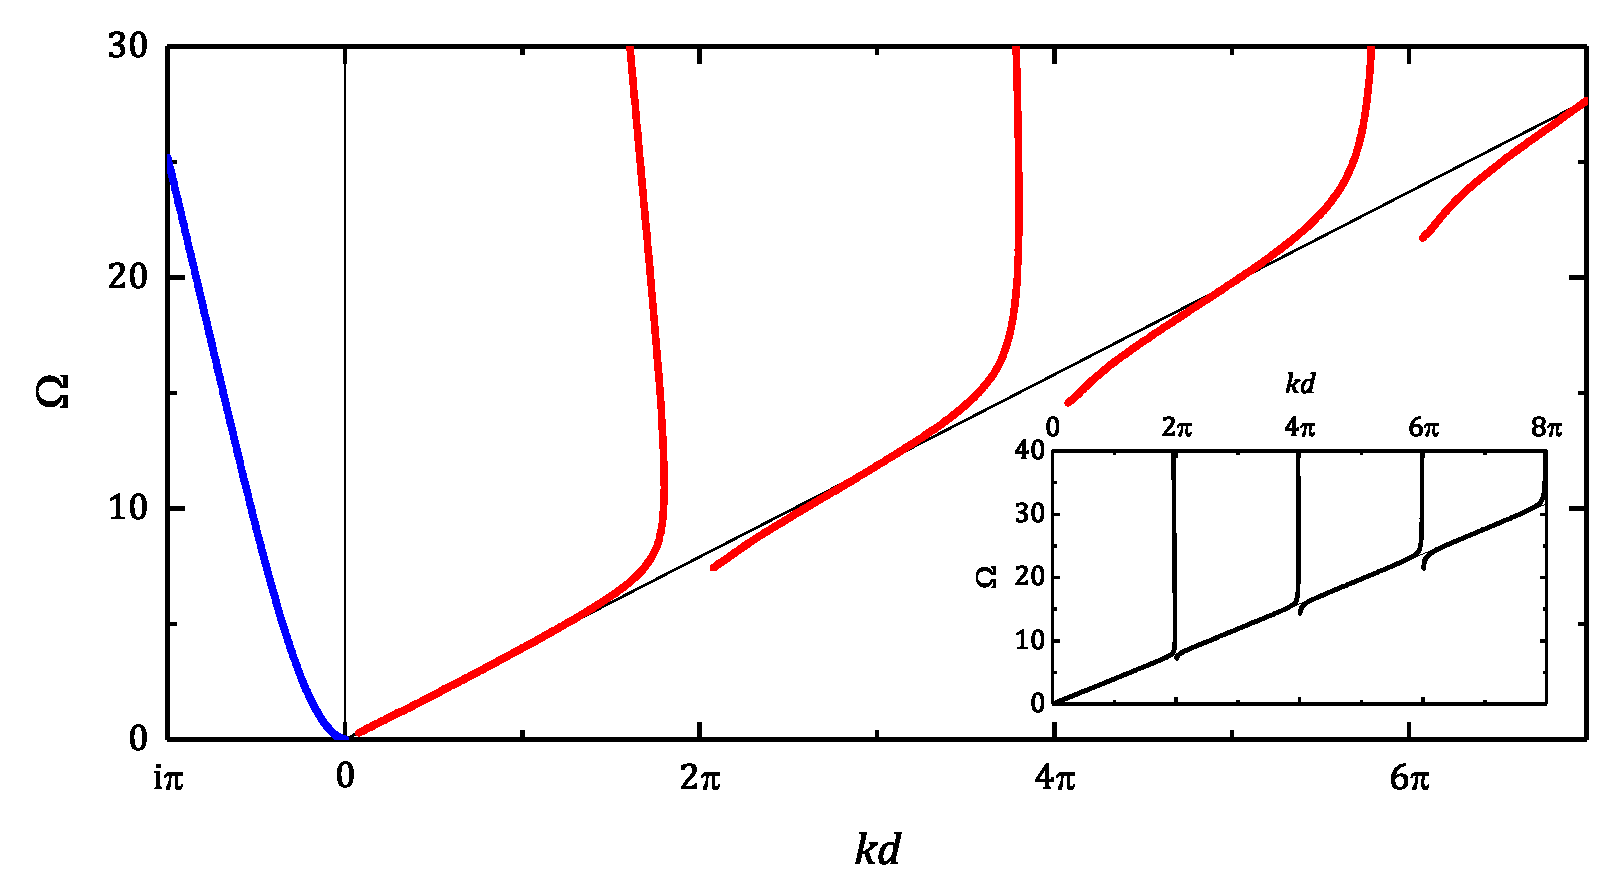
\includegraphics[width=\linewidth]{omega-kd.eps}
\caption{Dispersion relation between dimensionless frequency $\Omega=c_t \omega/d$ and transverse wavevector $kd/2$ obtained from \cref{eq:dispersionXiRayleigh} for the~infinite water channel between two brass plates, $\rho_f/\rho_m = 0.12$. The~linear dispersion for the~case of $\rho_f/\rho_m = 0$ (Rayleigh wave) is shown by a~thin line. The~inset shows the~dispersion of the~fast mode for very weak coupling, $\rho_f/\rho_m = 0.01$. In this case the~waveguide modes are reduced to almost vertical lines at $k d/2 = \pi n$. Dispersion of the~slow mode obtained from \cref{eq:dispersionXiRayleigh} for purely imaginary values of $k$ is plotted to the~left of the~origin.}
\label{fig:spectr}
\end{center}
\end{figure}


The~numerically calculated dispersion of the~real eigenmodes given by \cref{eq:dispersionkRayleigh} is shown in \cref{fig:xi-q} and \cref{fig:spectr}.
The~\cref{fig:xi-q} shows the~dimensionless phase speed $\xi$ versus the~wavevector $q$.
The~fast eigenmodes are enumerated by the~integer $n$, with the~lower number corresponding to the~branch with lower cutoff frequency.
The~slow mode is labeled by $0$.

All the~fast-mode branches lie between the~two horizontal lines, $\xi=c_f/c_t$ and $\xi=1$, and emerge at their corresponding cutoff frequency $\Omega_n$ given by \cref{eq:cutoffRayleigh}.
Close to the~level of the~phase velocity of the~Rayleigh wave, $\xi=\xi_R$, the~dispersion curves flatten and then become steep again.
Eventually, they saturate at the~level $\xi=c_f/c_t$.

The~line displaced below $\xi=c_f/c_t$ in \cref{fig:xi-q} represents the~slow Rayleigh mode.
This branch starts from zero frequency with zero phase speed.
For $q > 5$, the~phase speed already saturates to the~level $\xi=\xi_a$ given by \cref{eq:xiaRayleigh}.
This leaves only the~short subwavelength region, where the~phase speed grows rapidly.
In this region, the~channel width is smaller than the~wavelength of sound, $\lambda \geq 2 \pi d/5$, where the~wavelength is $\lambda=2\pi/\beta=2 \pi d/ q$.

In the~limit of very long wavelengths, $\lambda > 100 \pi d$, the~asymptotic approximation \cref{eq:asymptSlowRayleigh} is valid and agrees well with the~numerically calculated spectrum.

% The~ phase velocity of this mode grows extremely fast, starting from zero and approaching $c_f$ for $q > 5$. The~growth occurs in the~subwavelength region, where the~wavelength $\lambda=2\pi/\beta=2 \pi d/ q$ is  greater than the~channel width, $\lambda \geq 2 \pi d/5$. This narrow subwavelength region is zoomed in the~insert to \cref{fig:xi-q}. Within this region the~frequency $\Omega$ and wavevector $q$ are small parameters. Expansion of \cref{disp} leads to the~following nonlinear dispersion in the~low-frequency limit:
 
%As shown in  \cref{fig:xi-q}, this asymptotics is valid in the~region of very long wavelengths, when $\lambda > 100 \pi d$. It is this part of the~spectrum which provides penetration of sound through {\it any} narrow slit. Unlike transmission through a~channel with ideally rigid walls where the~dispersion is linear (see \cref{symm} for $n =0$), in a~real channel the~vibrations of the~walls result in nonlinear dispersion \cref{dispapprox} with vanishing phase and group velocities in the~low-frequency limit. Analysis of transmission through a~subwavelength acoustic channel will be published elsewhere.

The~\cref{fig:spectr} shows the~dimensionless frequency $\Omega$ versus $kd/2$.
Here the~horizontal axis does not represent the~wavevector in the~direction of propagation, and thus the~slope of the~curves is unrelated to either phase or group velocity.

For $\rho_f/\rho_m \ll 1$, the~dispersion of the~fast modes strictly follows the~linear Rayleigh wave dispersion (given by \cref{eq:dispNoRHSRayleigh}), except for the~points $kd/2=\pi n$ ($n=1,2,\dots$), where the~coupled Rayleigh waves become waveguide modes of the~channel with rigid walls.
The~dispersion curves are practically vertical for those values of $k$.

In the~case of $\rho_f/\rho_m = 0.12$, the~fast-mode branches emerge below the~Rayleigh wave dispersion \cref{eq:dispNoRHSRayleigh} and do not follow the~dispersion curves for either limiting case as accurately as it was for $\rho_f/\rho_m \ll 1$.

%The~asymptotes for the~dispersion branches of the~fast modes are the~linear dispersion of the~Rayleigh wave  and the~waveguide modes
%For almost all values of $kd/2$ the~right-hand side of \cref{eq:dispersionkRayleigh} can be neglected since $\rho_f/\rho_m <<1$. In this approximation \cref{eq:dispersionkRayleigh} gives linear dispersion (Rayleigh wave) which serves as asymptote for the~dispersion curves of the~fast mode. However, near the~points where $kd/2=\pi n$ ($n=1,2,\dots$) the~Rayleigh wave becomes a~waveguide mode of a~channel with rigid walls. Here the~dispersion curves become practically vertical lines as a~result of quantization condition $v_z=\frac{\partial B}{\partial z}|_{z = \pm d/2}=0$. For very small ratio $\rho_f/\rho_m= 0.01$ the~spectrum exhibits this quantization condition with high accuracy, as one can see in the~inset to \cref{fig:spectr}.

The~slow mode is plotted separately since it is characterized by purely imaginary values of $k$ in \cref{eq:dispersionkRayleigh}.
For the~sake of visualization, the~corresponding values of $k$ are plotted along the~negative direction of the~horizontal axis.
When the~value of $k$ is large, $|k|d/2 \gg 1$, the~dispersion of the~slow mode becomes practically linear.


\subsection{Complex Eigenmodes}

The~dispersion equation \cref{eq:dispersionXiRayleigh} has an~infinite number of complex roots with $\re\xi~>~0$ for any frequency $\omega=\Omega d/c_t$ (which is assumed to be purely real).
The~wavevectors $\beta$ of the~corresponding coupled Rayleigh waves acquire imaginary part, $\beta = \omega/c_t\xi = \beta'+i\beta''$.
As a~result, the~eigenmodes either exponentially grow or decay as they propagate into the~channel, as described by the~term $e^{i\beta x}=e^{i\beta'x-\beta''x}$ in the~acoustic potentials.
Since the~exponential growth of the~amplitude is physically unreasonable, only the~roots with $\xi''=\im \xi < 0$ must be considered in order to guarantee that $\beta'' > 0$.

The~decay of the~eigenmode into the~channel implies that the~acoustic energy is radiated away from the~channel (as the~media themselves are lossless).
The~Rayleigh wave in the~solid plates must then be a~propagating wave in $z$-direction, which can be realized if the~coefficients $\nu$ and $\eta$ acquire imaginary parts as well.
Indeed, from the~definitions \cref{eq:nuRayleigh}-\cref{eq:etaRayleigh} it is clear that both $\nu$ and $\eta$ are complex if the~wavevector $\beta$ is complex.
By analyzing the~terms in the~potentials \cref{eq:potLcoupledRayleigh}-\cref{eq:potScoupledRayleigh} that describe the~$z$ dependence, $e^{-\nu z}=e^{-\nu'z-i\nu''z}$ and $e^{-\eta z}=e^{-\eta'z-i\eta''z}$, one can see that the~imaginary parts of both coefficients $\nu$ and $\eta$ must be negative.
Moreover, their real parts need to be negative as well.
The~Rayleigh wave amplitude will then oscillate and exponentially grow along $z$ and oscillate and exponentially decay along $x$.
Such inhomogeneous plane wave is a~so-called leaky wave, which radiates energy in the~direction at a~certain angle from the~channel.
It also maintains constant amplitude along that direction due to the~mutual balancing of the~exponential grow and decay along $z$ and $x$.

It is crucial, however, to specify how the~square roots in these definitions need to be calculated in order to ensure the~desired propagating behavior along $z$.
One way to redefine coefficients \cref{eq:nuRayleigh} and \cref{eq:etaRayleigh} to ensure the~leaky-wave behavior is to choose a~second branch of the~complex square root function:
\begin{align}
\nu~&=~-\sqrt{\beta^2-k_l^2}, &\re\beta \ge k_l=\frac{\omega}{c_l}, \label{eq:numinusRayleigh}\\
\eta~&=~-\sqrt{\beta^2-k_t^2}, &\re\beta \ge k_t=\frac{\omega}{c_t}. \label{eq:etaminusRayleigh}
\end{align}
A~more detailed discussion on the~leaky waves and the~corresponding revision of the~square root function can be found in Appendix \ref{appBranchCut}.

The~dispersion equation for the~coupled Rayleigh leaky modes will then differ from \cref{eq:dispersionXiRayleigh} by having an~additional negative sign in its right-hand side:
\begin{equation}
\label{eq:dispersionXiLeakyRayleigh}
\left(2-\xi^2\right)^2-4\sqrt{1-\xi^2}\sqrt{1-\frac{c_t^2}{c_l^2}\xi^2}
~=~-\frac{\rho_f}{\rho_m}\,\xi^4 \sqrt{\frac{1-\left(c_t/c_l\right)^2\xi^2}{\left(c_t/c_f\right)^2\xi^2-1}}\cot\!\left(\frac{\Omega}{2\xi}\sqrt{\frac{c_t^2}{c_f^2} \xi^2-1}\,\right).
\end{equation}


\begin{figure}
\begin{center}
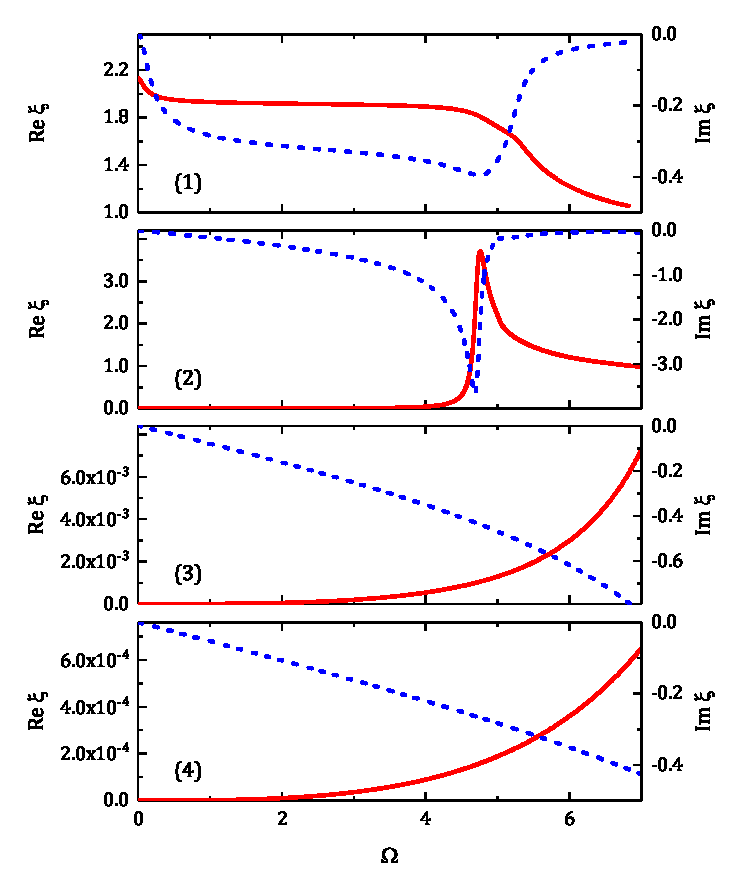
\includegraphics[width=0.85\linewidth]{ComplexRoots.eps}
\caption{Frequency dependence of the~first four complex roots of the~dispersion equation \cref{eq:dispersionXiLeakyRayleigh} for a~water channel between two brass plates. The~real and imaginary parts of each root are shown with solid red and dashed blue curves, respectively.}
\label{fig:roots}
\end{center}
\end{figure}


The~frequency dispersion of several complex roots of \cref{eq:dispersionXiLeakyRayleigh} is shown in \cref{fig:roots}.
These roots are ordered according to their imaginary parts, meaning that they are assigned the~ordinal number $n$ to satisfy the~ordering $
\im\beta_{n} < \im\beta_{n+1}$.
The~first complex root has a~negligible imaginary part at low frequencies.
Because of that, the~corresponding weakly leaky mode contributes to subwavelength transmission of sound through the~metal plates and can compete with the~transmission through the~channel via the~slow Rayleigh mode.

Note that in the~limit of zero channel width there must be a~quasi-longitudinal Rayleigh mode.
Such mode should be only a~slight modification of a~pure longitudinal wave that propagates in the~bulk of the~solid.
Obviously, none of the~real Rayleigh eigenmodes fits this role as their phase speeds are smaller that $c_t$ ($\xi \le 1$).
This means that a~pure longitudinal wave cannot propagate in a~solid plate with a~slit: the~longitudinal vibrations lead to the~inevitable shear displacements in the~solid in the~vicinity of the~slit.
The~corresponding Rayleigh eigenmode must then be necessarily complex and, actually, the~first leaky mode is the~eigenmode in question.
Indeed, in the~limit of zero frequency the~real part of its phase speed approaches $\re\xi = c_l/c_t$, which exactly corresponds to the~speed of longitudinal waves, and its imaginary part vanishes.
Consequently, when considering the~transmission of sound through a~finite sample, the~first leaky mode will be responsible for the~maxima in the~transmission spectrum that would resemble the~Fabry-Perot maxima for the~bulk plate of the~same thickness.

\subsection{Eigenmode Orthogonality}

An~eigenmode (eigenfunction) $f_n$ of a~physical system is always a~nontrivial solution of a~certain \textit{homogeneous} problem, in which there is no external influence on the~system.
The~set of eigenmodes forms a~complete basis in the~function space.
Then any process (given by a~function $f$) occurring in the~system can be represented as a~superposition of the~eigenmodes, or in other words, it can be expanded over the~known basis:
\begin{equation}
\label{eq:basisRayleigh}
f~=~\sum C_n f_n.
\end{equation}
The~coefficients of the~expansion can easily be found if the~eigenmodes are orthogonal:
\begin{equation}
\langle f_n, f_m \rangle~=~||f_n||^2\delta_{n,m}.
\end{equation}
Here the~term in the~left-hand side is a~generalized inner product of two eigenmodes, $||\cdot||$ gives the~norm of its argument, and $\delta_{n,m}$ is the~Kronecker symbol.
The~coefficients of the~expansion $C_m$ are then immediately obtained as
\begin{equation}
C_m~=~\frac{\langle f, f_m\rangle}{||f_m||^2}.
\end{equation}

For the~problem of sound transmission through a~finite-sized fluid channel between two metal plates, determining the~unknown coefficients in the~expansion of the~signal over the~coupled Rayleigh modes will be crucial for obtaining the~solution.
However, the~Rayleigh eigenmodes are not orthogonal, for the~reason that the~boundary conditions at the~fluid-solid interface \cref{eq:coeffRelationsRayleigh} explicitly contain the~wavevector $\beta$ \cite{bobrovnitskii}.
Moreover, the~eigenmodes of any problem where the~elastic waves are confined to a~finite volume are known to be nonorthogonal.
For example, the~Lamb waves (normal vibrations) in an~elastic slab are not mutually orthogonal over the~slab width \cite{lyon}.
Even though a~lot of efforts were put to redefine the~orthogonality for Lamb waves from the~reciprocity principles \cite{bobrovnitskii,achenbac,zakharov,folk}, the~proposed new relations do not facilitate calculating the~coefficients of the~expansion $C_m$. 

The~nonorthogonal basis can always be transformed into an~orthogonal one by, e.g., employing the~Gram-Schmidt procedure, however, I will not be using this procedure for several reasons.
One of them is that this orthogonalization process is quite difficult to perform in regards to the~Rayleigh eigenmodes, and using it would significantly increase the~complexity of the~problem.
Another reason is that it will be much easier to calculate the~unknown coefficients $C_m$ if one expands both the~function $f$ and the~eigenmodes $f_n$ over some simple orthogonal basis $g_n$:
\begin{equation}
f~=~\sum f^{(m)}g_m, \qquad f_n~=~\sum f_n^{(m)}g_m,
\end{equation}
with the~coefficients $f^{(m)}$ and $f_n^{(m)}$, respectively. 
After substituting the~latter relations to \cref{eq:basisRayleigh} and calculating the~inner product with every $g_m$ for each part of the~equation, the~following set of equations is obtained:
\begin{equation}
f^{(m)}~=~\sum C_n f_n^{(m)}.
\end{equation}
The~linear system can now be solved numerically, for example.
This discussion clearly shows that the~use of the~nonorthogonal basis is not too much of an~inconvenience in solving a~problem.

%It is well-known that an~eigenvalue problem for elastic waves in a~finite volume leads to a~set of nonorthogonal eigenfunctions. In particular, normal vibrations of elastic plate (Lamb waves) are not orthogonal over the~width of the~plate \cite{lyon}.  While several "orthogonality relations" for Lamb waves based on the~reciprocity relations have been proposed \cite{bobrovnitskii,achenbach}, they (or their modification for solid-fluid structure \cite{zakharov}) cannot help in calculation of $b_n^{\pm}$.

%The~right-hand-sides of Eqs. \cref{eq:app_22} and \cref{eq:app_23} are presented in the~form of expansions over eigenfunctions of vibrating fluid channel. These eigenfunctions are defined on the~semiaxis $z>0$. They are oscillating, $\cos(k_nz)$, within the~channel, $0<z<d/2$, and evanescent, $\exp(-\eta_n z)$, $\exp(-\nu_n z)$, inside the~metal plates, $z> d/2$. These eigenfunctions, as well as the~displacements and velocities defined by them, are not orthogonal. The~lack of orthogonality is due to the~boundary conditions at $z= \pm d/2$, explicitly containing the~eigenvector $\beta_n$, as it was mentioned in Ref. \cite{bobrovnitskii} with respect to non-orthogonality of Lamb modes in a~solid plate.

%While the~non-orthogonal basis does not allow analytical calculation of the~unknowns $b_n^{\pm}$, it really does not impose additional difficulty in numerical calculation. \textbf{On the~contrary, using orthogonal basis would be less appropriate, because orthogonalization of the~naturally introduced non-orthogonal basis of channel eigenfunctions is itself a~procedure of greater difficulty than solving an~inhomogeneous system of linear equations in the~method shown below}. Due to the~fact that the~size of the~set of equations \cref{eq:app_22} and \cref{eq:app_23} is cut by the~number of calculated roots $\xi_n(\omega)$, $n =1,2,\dots, N$, the~necessary set of equations for $b_n^{\pm}$ can, for example, be obtained by equating the~first $N$ Fourier coefficients of the~both sides of Eqs. \cref{eq:app_22} and \cref{eq:app_23}. We introduce the~finite Fourier transform defined on a~segment $0<z<R_d$.

% to stress that the~Fabry-Perot maxima in transmission are due to the~roots which are necessary complex. Indeed, these maxima appear when longitudinal waves interfere constructively at the~length $h$. Since $c_l>c_t$, the~roots of the~dispersion equation which correspond to the~phase velocities close to $c_l$ cannot lie within the~interval $0<\xi \leq 1$ (where all the~real roots lie), i.e. they are all complex. This complexity reflects an~obvious fact that in a~solid plate with a~slit pure longitudinal waves cannot propagate. Even a~narrow slit gives rise to shear displacements which change the~amplitude and phase of the~Fabry-Perot resonance. The~imaginary part of the~quasi-longitudinal solution may be quite small which means only slight modification of the~Fabry-Perot resonance. For example, the~complex root shown in Fig.~\cref{fig:roots} has the~real part close to 2 (which is approximately the~ratio $c_l/c_t$ in brass) and negligible imaginary part in the~limits of either zero frequency or zero channel width. This root corresponds to quasi-longitudinal sound wave propagating in metal.


%%%%%%%%%%%%%%%%%%%%%%%%%%%%%%%%%%%%%%%%%%%%%%%%
%%%%%%%%%%%%%%%%%%%%%%%%%%%%%%%%%%%%%%%%%%%%%%%%
%%%%%%%%%%%%%%%%%%%%%%%%%%%%%%%%%%%%%%%%%%%%%%%%
%%%%%%%%%%%%%%%%%%%%%%%%%%%%%%%%%%%%%%%%%%%%%%%%
% A~solution of the~wave equation in the~fluid and in the~plates can be written as a~superposition of the~corresponding eigenmodes \cref{pot}. Linear relations between the~coefficients $b_n$, $l_n$, and $s_n$ are obtained from the~boundary conditions. Since the~channel is infinite we can consider only the~waves propagating in positive direction of axis $x$ and omit super-indices $\pm$.
%
%At the~fluid-metal interface $z=d/2$ 
%Here $\sigma_{ik}(x,z)$ is the~stress tensor in the~elastic plates.
%%and it was taken into account that the~stress tensor for ideal fluid is diagonal,
%%$\sigma^{(f)}_{ik}=-p\delta_{ik}$.
%Using the~Hooke's Law $\sigma_{ik}~=~\lambda u_{ll}\delta_{ik} + 2\mu u_{ik}$
%the~nonzero components of the~stress tensor can be expressed through the~potentials
%\begin{align}
%\label{8}
%\sigma_{xx}~&=~-\lambda k_l^2 L +2\mu\left(\frac{\partial^2 L}{\partial x^2}-\frac{\partial^2 S}{\partial x \partial z}\right), \\
%\sigma_{zz}~&=~-\lambda k_l^2 L +2\mu\left(\frac{\partial^2 L}{\partial z^2}+\frac{\partial^2 S}{\partial x \partial z}\right), \notag \\
%\sigma_{xz}~&=~\mu\left(2\frac{\partial^2 L}{\partial x \partial z}+\frac{\partial^2 S}{\partial x^2}-\frac{\partial^2 S}{\partial z^2}\right). \notag
%\end{align}
%Here $\lambda$ and $\mu$ are the~Lam{\'e} coefficients, $\mu~=~\rho_m c_t^2, \,\, \lambda+2\mu~=~\rho_m c_l^2$. Substituting the~potentials  \cref{pot} to \cref{8} and \cref{dispvec}, the~components of $\sigma_{ik}$ and $\bf u$ are expressed through the~unknown constants $l_n$ and $s_n$.  The~velocity ${\bf v} = \nabla B$ and the~pressure $p=i\omega \rho B$ are expressed through $b_n$. Thus, all the~dynamical variables are given in terms of three unknowns, $l$, $s$, and $b$.

%The~boundary conditions \cref{7} written in terms of $l$, $s$, and $b$ (here sub-index $n$ can be omitted) lead to the~following set of linear equations:
%\begin{equation}
%\label{10}
%\left\{
%\begin{aligned}
%&\left(2\mu\nu^2-\lambda k_l^2\right)\,e^{-\nu d/2}\cdot l
%- 2i\mu \eta \beta\,e^{-\eta d/2}\cdot s+i\omega\rho_f \cos(k d/2)\cdot b~&=~0, \\
%&2i\nu \beta \,e^{-\nu d/2}\cdot l+ e^{-\eta d/2}\left(\beta^2 +\eta^2 \right) \cdot s ~&=~0, \\
%&k \sin(k d/2)\cdot b+i\omega\nu \,e^{-\nu d/2}\cdot l +\omega\beta \,e^{-\eta d/2}\cdot s~&=~0.
%\end{aligned}
%\right.
%\end{equation}
%This set has nontrivial solution if the~corresponding determinant vanishes, viz
%\begin{equation}
%\label{11}
%\left(\eta^2+\beta^2\right)^2-4\nu\eta\beta^2~=~\frac{\rho_f}{\rho_m}\frac{\omega^4}{c_t^4}\frac{\nu}{k}\,\cot \frac{kd}{2}.
%\end{equation}
%Here $k$, $\nu$, and $\eta$ are expressed through $\omega$ and $\beta$ using \cref{kk}.
%Dependence on the~channel width $d$ can be eliminated if dimensionless frequency $\Omega = \omega d/c_t$ and wave vector $q = \beta d$ are introduced.
%\begin{equation}
%\label{disp2}
%\left(2 q^2-\Omega^2\right)^2 - 4 q^2 \sqrt{q^2 - (c_t/c_l)^2 \Omega^2} \sqrt{q^2 - \Omega^2} 
%~=~ \frac{\rho_f}{\rho_m}\Omega^4 \sqrt{\frac{q^2 - (c_t/c_l)^2 \Omega^2}{(c_t/c_f)^2 \Omega^2 - q^2}}\,\cot( \frac{1}{2}\sqrt{\frac{c_t^2}{c_f^2} \Omega^2 - q^2}).
%\end{equation}
%Dispersion relation \cref{disp} for the~phase velocity $\xi$ is obtained from \cref{disp2} by substitution $q=\Omega /\xi$. Real and complex solutions of \cref{disp2} define the~allowed values of the~wave vector $q_n= q_n(\Omega)$ for each frequency $\Omega$.




%Expansions \cref{pot} of the~potentials over eigenmodes can be used if all real roots and sufficient number of complex roots of the~dispersion equation \cref{disp} are known. In general case each root depends on frequency, $\xi_n=\xi_n(\omega)$ that shows frequency dispersion of the~corresponding mode. Examples of frequency dispersion for the~lowest two real solutions are given in the~left panel in \cref{fig:roots}. The~mode which starts at $\omega = 0$ is the~slow mode (blue line). It exhibits strong dispersion in the~subwavelength regime and at $\omega > 0.5$ MHz the~phase velocity saturates at the~level $\xi=c_f/c_t$, i.e the~slow mode becomes dispersionless sound wave, propagating with speed $c_f$. Red line shows dispersion of the~first waveguide mode. This mode starts at cut-off frequency $(c_t/d) \Omega_1$. 


%%%%%%%%%%%%%%%%%%%%%%%%%%%%%%%%
%{The~eigenmodes in  \cref{pot} are labeled by integer $n$ which numerates the~roots of the~dispersion equation $\beta_n = \beta_n(\omega)$. This equation is derived in Appendix \ref{appRayleigh} from the~continuity of force and velocity at the~boundaries $z= \pm d/2$ \cite{adv,Lloyd}. Since the~system is symmetric with respect to the~plane $z=0$ the~eigenmodes are either even or odd functions of $z$. Odd modes are excited at oblique incidence or if the~plates are made of different metals \cite{channel1}. In our case only even modes can be excited. The~dispersion equation for these modes is written as follows:
%\begin{equation}
%\label{disp}
%\left(2-\xi^2\right)^2-4\sqrt{1-\xi^2}\sqrt{1-\frac{c_t^2}{c_l^2}\xi^2}
%~=~\pm\frac{\rho_f}{\rho_m}\,\xi^4 \sqrt{\frac{1-\left(c_t/c_l\right)^2\xi^2}{\left(c_t/c_f\right)^2\xi^2-1}}\cot\!\left(\frac{\omega}{\xi}\frac{d}{2c_t}\sqrt{\frac{c_t^2}{c_f^2} \xi^2-1}\,\right).
%\end{equation}
%Here $\rho_m$ is the~density of the~elastic plates plates. Each root $\xi_n$ of the~dispersion equation gives the~normalized phase velocity $\xi_n = \omega/ c_t \beta_n$ of the~coupled quasi-surface waves. Since the~coupling between these  waves occurs through the~fluid, the~r.h.s of \cref{disp} is proportional  to the~ratio $\rho_f/\rho_m$. When $\rho_f/\rho_m = 0$ the~vibrations of the~plates are uncoupled and \cref{disp} is reduced to the~well-known cubic equation with respect to $\xi^2$. Its unique solution $\xi = \xi_R$ defines the~velocity of dispersionless surface Rayleigh wave at the~plane interface between vacuum and elastic solid \cite{viktor}.}
%
%{The~dispersion equation has finite number of real roots
%and infinite number of complex roots with  $\mathrm{Re}\xi_n > 0$. {\bf Due to the~factor $\sqrt{1-\xi^2}$ all real roots lie within the~interval $0<\xi \leq 1$.} The~real roots are obtained from  \cref{disp} with "+" sign in the~right-hand side. Each complex root  gives rise to an~inhomogeneous plane wave in the~expansions \cref{pot}. These terms oscillate and decay with the~coordinate $z$. For complex roots the~decrements $\nu_n$ and $\eta_n$ acquire imaginary parts, which must be negative  in order the~corresponding modes run {\it away} from the~channel. This scattering condition is satisfied for the~roots with $\mathrm{Im}\xi_n < 0$, which are obtained from \cref{disp} with "-" sign in the~right-hand side. For each
%frequency $\omega$ all the~real roots must be included in the~expansions \cref{pot}. The~number of complex roots included in numerical calculations depends on
%desired accuracy. The~roots are arranged in ascending order of the~imaginary part of the~longitudinal wave vector $\beta_n = \omega/(c_t \xi_n)$ ($|\mathrm{Im} \beta_{n-1}| < |\mathrm{Im} \beta_n|$), since those with smaller $|\mathrm{Im} \beta|$ give larger contributions.  For infinitely long channel the~complex solutions should be ignored as they decay exponentially with length, but they play essential role in sound transmission through a~finite-length channel.}

%{Solutions of the~transcendental equation \cref{disp} are obtained numerically. For channel of width $d$ \cref{disp} gives implicit relation between the~dimensionless phase velocity $\xi$ and frequency $\omega$. Substituting $\omega = (c_t/d)\xi q$, where $q=\beta d$ is dimensionless wave vector, into the~argument of cotangent in \cref{disp}, we obtain equation which relates the~dimensionless phase velocity $\xi$ and wave vector $q$. This equation is independent of the~channel width $d$ and it leads to the~spectrum shown in \cref{fig:xi-q}.
% The~spectrum consists of two unequal parts. One is so-called {\it fast mode} propagating faster than sound wave in the~fluid, $\xi>c_f/c_t$. It has infinite number of branches (shown in red) which originate from the~symmetric waveguide modes
%\begin{equation}
%\label{symm}
%\omega_n = c_f \sqrt{\left(\frac{2\pi n}{d}\right)^2+\beta^2}, \,\,\, n = 0,1,2,\dots
%\end{equation}
%of a~channel with ideally rigid walls, $\rho_m, c_t \rightarrow \infty$. More detailed analysis of the~spectrum in the~limit $\rho_f/\rho_m \rightarrow 0$ is given in Appendix \ref{appRayleigh}. All the~branches of the~fast mode lie between two horizontal lines, $c_f/c_t < \xi \leq 1$. Unlike the~waveguide spectrum \cref{symm} where each phase velocity $\omega_n/\beta$ diverges at $\beta = 0$, except the~mode with $n = 0$, in a~channel with elastic boundaries all fast modes start with finite phase velocity $\xi = 1$ at the~wavevector
%\begin{equation}
%\label{veloc}
%Q_n = \beta_n d= \frac{2}{\sqrt{(c_t/c_f)^2 -1}} \left[ \pi n +
%\arctan\left(\frac{\rho_f}{\rho_m} \sqrt{\frac{1-(c_t/c_l)^2}{(c_t/c_f)^2-1}}\, \right)\right] ,\,\, n = 0,1,2, \dots
%\end{equation}
%Near the~point where each branch crosses the~level of the~phase velocity of the~Rayleigh wave, $\xi=\xi_R$, the~slope of the~dispersion curve noticeably decreases since for the~parameters used in the~plot of \cref{fig:xi-q} the~ratio  $\rho_f/\rho_m=0.12$ is quite small.}
%
%{Another part of the~spectrum in \cref{fig:xi-q} is represented by a~blue line. It is displaced below the~level $\xi=c_f/c_t$, i.e. this mode propagates slower than sound in the~fluid. The~right-hand side of the~dispersion equation \cref{disp} remains real while the~square root $\sqrt{(\frac{c_t}{c_f})^2 \xi^2 -1}$ is pure imaginary. The~ phase velocity of this mode grows extremely fast, starting from zero and approaching $c_f$ for $q > 5$. The~growth occurs in the~subwavelength region, where the~wavelength $\lambda=2\pi/\beta=2 \pi d/ q$ is  greater than the~channel width, $\lambda \geq 2 \pi d/5$. This narrow subwavelength region is zoomed in the~insert to \cref{fig:xi-q}. Within this region the~frequency $\Omega$ and wavevector $q$ are small parameters. Expansion of \cref{disp} leads to the~following nonlinear dispersion in the~low-frequency limit:
%\begin{equation}
%\label{dispapprox}
%\Omega \approx {\sqrt{\frac{\rho_m}{\rho_f}\left(1-\frac{c_t^2}{c_l^2}\right)}}\, (\beta d)^{3/2}.
%\end{equation}
%As shown in  \cref{fig:xi-q}, this asymptotics is valid in the~region of very long wavelengths, when $\lambda > 100 \pi d$. It is this part of the~spectrum which provides penetration of sound through {\it any} narrow slit. Unlike transmission through a~channel with ideally rigid walls where the~dispersion is linear (see \cref{symm} for $n =0$), in a~real channel the~vibrations of the~walls result in nonlinear dispersion \cref{dispapprox} with vanishing phase and group velocities in the~low-frequency limit. Analysis of transmission through a~subwavelength acoustic channel will be published elsewhere. It is noteworthy to mention that transmission of electromagnetic waves through a~deeply subwavelength metallic slit also exhibits interesting features which do not exist for perfectly conducting screens \cite{Seo,Xia}}.


%%%%%%%%%%%%%%%%%%%%%%%%%%%%%%%%%%%%%%%%%%%%%%%%%%%%%%%%%%%%%%%%%%%%
\section{Scattering Problem}

The~knowledge of the~eigenmodes of the~infinite fluid channel allows to tackle the~problem of sound transmission through a~finite sample.
Namely, the~acoustic field inside the~channel and the~plates can be now expressed as a~superposition of the~channel eigenmodes.
In this approach the~boundary conditions at the~channel walls are automatically satisfied.
Also, one obtains a~practically exact analytical solution since the~acoustic potentials account for the~\textit{total} field at any given point.

The~only limiting factor here is the~number of the~eigenmodes used in the~potentials expansion.
The~exact solution requires writing an~infinite series over all possible eigenmodes.
Practically, the~series in question converges quite fast and it is sufficient to consider only the~first few of the~coupled Rayleigh eigenmodes.

\subsection{Geometry}

I will be considering a~problem that closely imitates the~conditions of the~experiment reported in \cite{channel1}.
In this experiment, two brass or aluminum plates of length $L=12$ cm and thickness $h$ were separated by a~distance $d$ (the~slit aperture).
The~system was immersed in a~water tank, and two transducers
of diameter $2R_d=1.5^{\prime\prime}$ were used to produce and detect the~sound.
Both transducers were positioned at a~distance $l=8$ cm from the~plates, centered with respect to the~channel, and the~sound was incident normally on the~slit.
This experimental setup is schematically shown in \cref{fig:geometryRayleigh}, as well as the~values of $d$ and $h$ for which the~experiment was performed.
Note that the~gravity is acting along the~$y$-direction.
Any effect of gravity is, however, omitted and the~problem is assumed uniform along the~$y$-axis.

\begin{figure}
\begin{center}
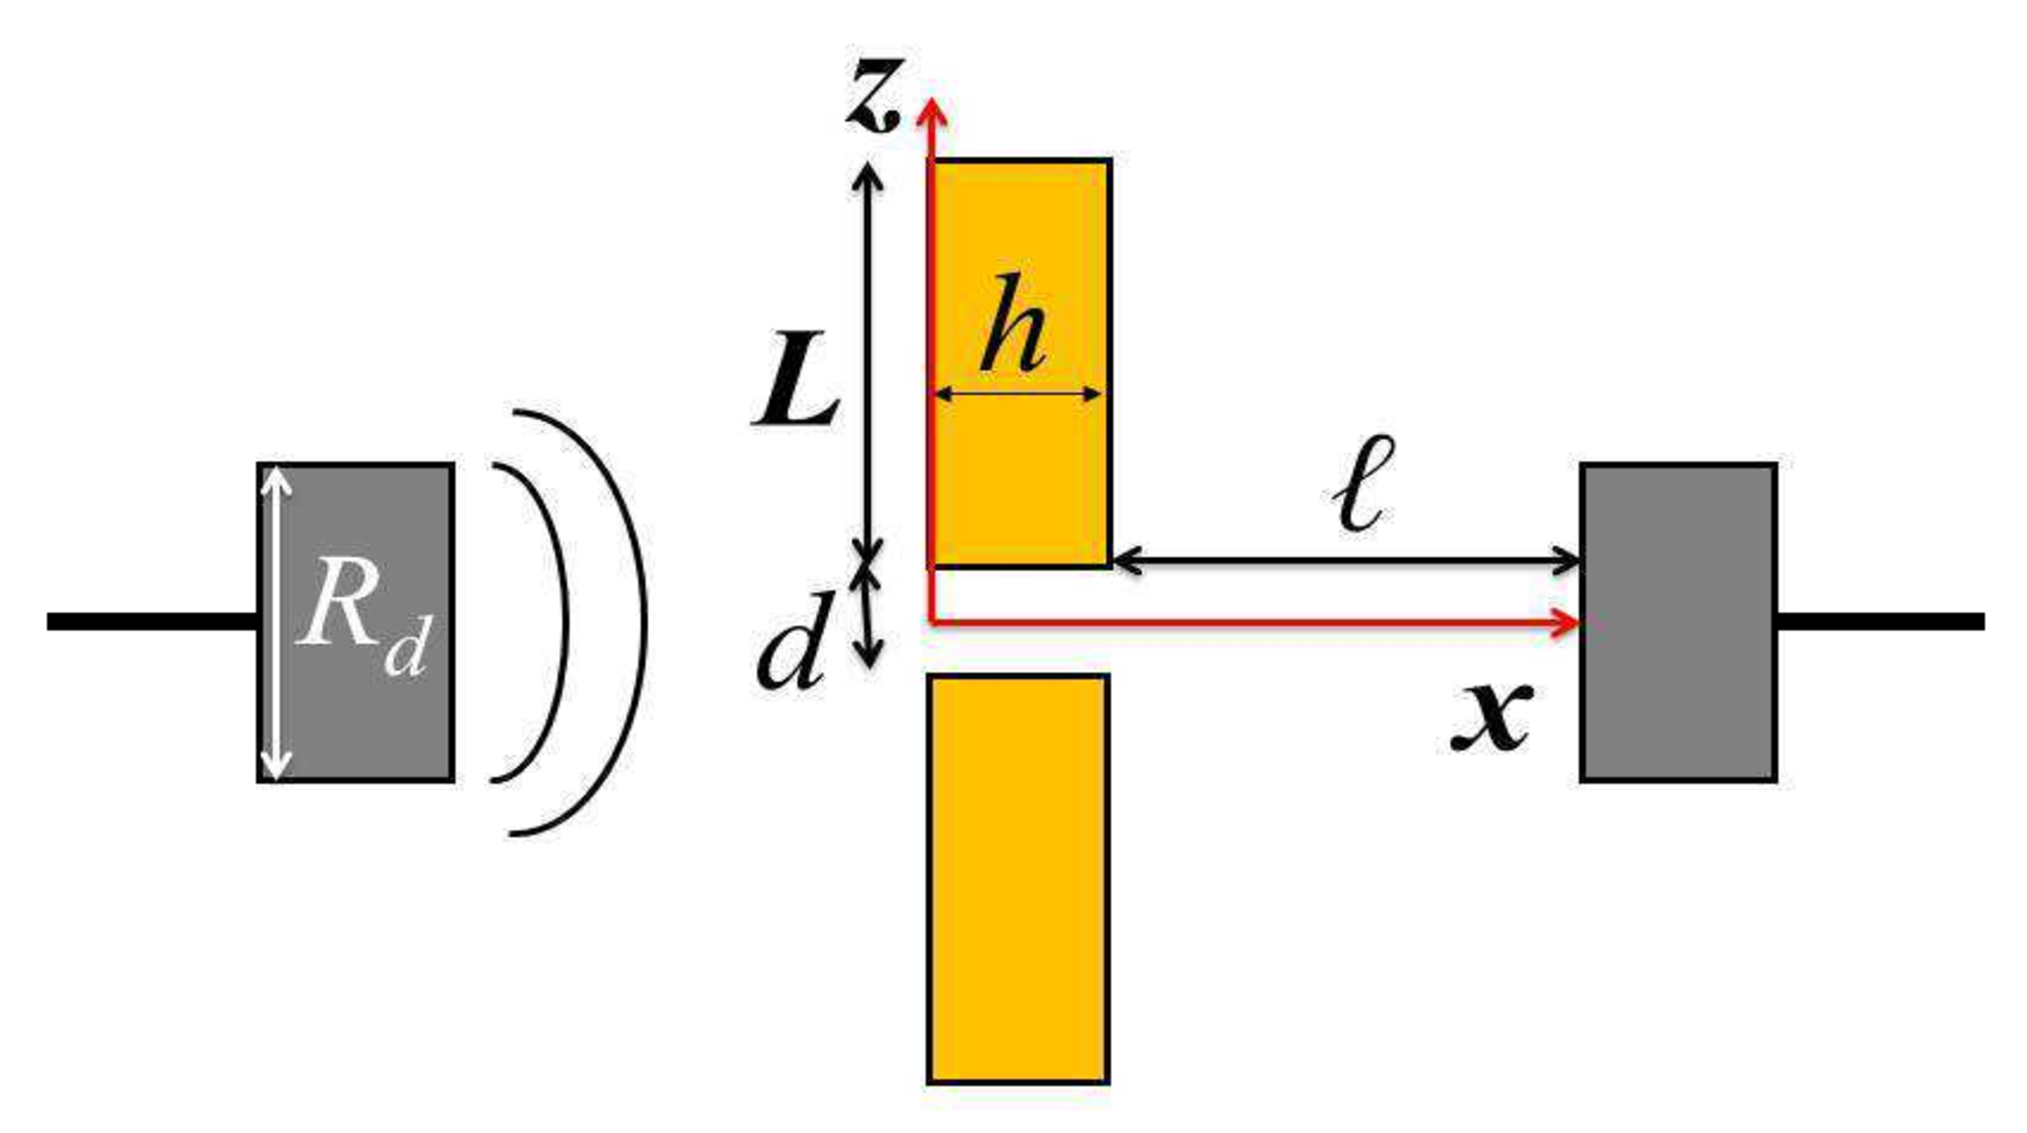
\includegraphics[width=0.85\linewidth]{fig0_geometry.eps}
\caption{Experimental setup showing the~geometrical parameters of the~fluid channel between the~metal plates and the~configuration of transducers.}
\label{fig:geometryRayleigh}
\end{center}
\end{figure}

Since the~size of each transducer is much larger than the~channel width, $d \ll R_d$, I will model the~incoming sound by a~plane wave. 


% a~sound wave was generated and detected by two $1.5^{\prime\prime}$ transducers immersed in a~water tank at equal distance  $l=8$ cm from the~plates. A~slit between two square brass or aluminum plates with side $L = 12$ cm is located in front of the~ transducers. A~sound wave was incident normally to the~slit and the~transmission spectrum was measured with compensation of the~non-flat frequency response of the~piezoelectric transducers. The~plate thickness $h$ defines the~length of the~water channel and its width $d$ (the~slit's aperture) is maintained by means
%of a~sample holder that fixes both metal plates. This experimental setup is schematically shown in the~inset to \cref{fig:experimentRayleigh}.

\subsection{Acoustic Potentials of Transmitted and Reflected Waves}

The~plane acoustic wave that is normally incident on the~slit and the~plates from the~left is described by the~acoustic potential $(p_0/i \omega \rho_f) \exp(ik_fx-i\omega t)$.
The~reflected and the~transmitted acoustic fields are denoted as $R(x,z)$ ($x<0$) and $T(x,z)$ ($x>h$), respectively.
Since the~channel scatters the~sound in every possible direction, I write the~potentials $R(x,z)$ and $T(x,z)$ as Fourier integrals
\begin{align}
R(x,z)~&=~\int\limits_{-\infty}^{+\infty}r(k)e^{ikz-i\beta(\!k)x}dk, &x \leq 0, \label{refl}\\
T(x,z)~&=~\int\limits_{-\infty}^{+\infty}t(k)e^{ikz+i\beta(\!k)(x-h)}dk , &x \geq h, \label{transm}
\end{align}
where the~amplitudes $r(k)$ and $t(k)$ are
\begin{align}
r(k)~&=~\frac{1}{2\pi}\int\limits_{-\infty}^{+\infty}R(0,z)e^{-ikz}dz, \label{refl2}\\
t(k)~&=~\frac{1}{2\pi}\int\limits_{-\infty}^{+\infty}T(h,z)e^{-ikz}dz. \label{transm2}
\end{align}
The~longitudinal (along $x$) component of the~wave vector is defined as $\beta(k)=\sqrt{k_f^2-k^2}$ for $|k| < k_f$ and $\beta(k)=i\sqrt{k^2-k_f^2}$ for $|k| > k_f$.
Each Fourier integrals essentially represents a~combination of all possible plane ($|k| < k_f$) and evanescent ($|k| > k_f$) waves that contribute to either reflection or transmission.


%To calculate the~transmission of a~plane sound wave coming from the~left, $(p_0/i \omega \rho_f) \exp(ik_0x-i\omega t)$, we introduce the~potentials of the~reflected $R(x,z)$ ($x<0$) and transmitted $T(x,z)$ ($x>h$) acoustic fields. They define velocity and pressure in the~fluid (e.g. ${\bf v} = \nabla R$, $p = p_0+ i \omega \rho_f R$ for $x<0$). Here  $k_0=\omega / c_f$,  $\rho_f$ is the~density and $c_f$ is the~speed of sound in the~fluid.  The~potentials of the~reflected and transmitted fields are represented through their Fourier integrals
%\begin{equation}
%R(x,z)~=~\int\limits_{-\infty}^{+\infty}r(k)e^{ikz-i\beta(\!k)x}dk , \,\,\, x \leq 0,
%\label{refl}
%\end{equation}
%\begin{equation}
%\label{trans}
%T(x,z)~=~\int\limits_{-\infty}^{+\infty}t(k)e^{ikz+i\beta(\!k)(x-h)}dk , \,\,\, x \geq h.
%\end{equation}
%Here the~longitudinal (along $x$) component of the~wave vector is defined as $\beta(k)=\sqrt{k_0^2-k^2}$ for $|k| < k_0$ and $\beta(k)=i\sqrt{k^2-k_0^2}$ for $|k| > k_0$.
%The~Fourier components $r(k)$ and $t(k)$ are linearly related through the~boundary conditions.

In the~region $0 \leq x \leq h$, i.e., inside the~fluid channel and the~elastic plates, the~potentials are superpositions of forward and backward propagating eigenmodes of the~corresponding infinite channel:
\begin{align}
B(x,z)~&=~\sum\limits_{n} (b_n^+ e^{i\beta_nx}+b_n^- e^{-i\beta_nx})\cos{k_nz}, &|z| < d/2, \label{pot1} \\
L(x,z)~&=~\sum\limits_{n}({l_n^+}e^{i\beta_nx}+l_n^- e^{-i\beta_nx})e^{-\nu_n|z|}, &|z| > d/2, \label{pot2} \\
S(x,z)~&=~\sum\limits_{n}({s_n^+}e^{i\beta_nx}-{s_n^-}e^{-i\beta_nx})e^{-\eta_n|z|}, &|z| > d/2. \label{pot3}
\end{align}
The~summation runs over all possible eigenmodes (propagating and leaky) of the~system for a~given frequency.
The~superindices "$+$" and "$-$" indicate propagation in the~$+x$ or $-x$ direction.
The~potentials for the~backpropagating Rayleigh waves are obtained from those describing the~propagation forward by applying the~symmetry transformation $x\rightarrow -x$, $y\rightarrow -y$, which is essentially the~$180^{o}$ rotation around the~$z$-axis.

The~unknown amplitudes $t(k)$ and $r(k)$ in \cref{refl}-\cref{transm} and the~coefficients $b_n$, $l_n$, and $s_n$ in \cref{pot1}-\cref{pot3} can be determined after the~appropriate boundary conditions at both vertical ($x=0,h$) surfaces of the~structure are established.
%where ${B}$ is the~ velocity potential of the~fluid (${\bf v}(x,z)=\nabla B$, $|z| \leq d/2$) and the~potentials $L$ and $S$ give the~displacement vector in the~plates,
%\begin{equation}
%\label{dispvec}
%{\bf u}=\nabla L + \nabla \times (S {\bf \hat y}), \,\,\, |z| \geq d/2.
%\end{equation}
%The~transversal parts of the~wave vectors in the~fluid and in the~plates are defined as
%\begin{align}
%\label{kk}
%&k_n=\sqrt{k_0^2-\beta_n^2}, \\
%&\nu_n=\sqrt{\beta_n^2-k_l^2}, \notag \\
%&\eta_n=\sqrt{\beta_n^2-k_t^2},\notag
%\end{align}
%where $\mathrm{Re}\,(\nu_n,\eta_n)>0$, $k_{l,t}=\omega/c_{l,t}$, and $c_t$  ($c_l$) is the~speed of transversal (longitudinal) sound in the~plates.
%%Summation in \cref{pot} runs over the~roots of the~dispersion equation, both real and complex. 
%Our final goal is calculation of the~reflected and transmitted acoustic fields in the~fluid.
%%%%%%%%%%%%%%%%%%%%%%%%%%%%%%%%%%%%%%%%%%%%%%%%%%%%%%%%%%%%%%%%%%%%%%%%%%%%%%%%%%%%%%%%%%%%%%%%%%%%%%%%%%%%%%%%%%%%%%%%%%%%%%%%%%%%%%%%%%%%%%%%%%%%%%%%%%%
%                                                      FIGURE #2
%%%%%%%%%%%%%%%%%%%%%%%%%%%%%%%%%%%%%%%%%%%%%%%%%%%%%%%%%%%%%%%%%%%%%%%%%%%%%%%%%%%%%%%%%%%%%%%%%%%%%%%%%%%%%%%%%%%%%%%%%%%%%%%%%%%%%%%%%%%%%%%%%%%%%%%%%%%
%\begin{figure}
%\begin{center}
%%\includegraphics[width = 9cm]{fig2.eps}
%\caption{ Dimensionless phase velocity $\xi=\Omega/q$ vs wave vector $q=\beta d$ for infinite brass channel filled by water. Fast mode is presented by infinite number of waveguide branches above the~speed of sound in water, $c_f/c_t< \xi < 1$ (red curves). Phase velocity of the~slow mode grows very fast (blue line near the~vertical axis) and saturates at the~level $\xi= c_f/c_t$ for very small $q= \beta d \approx 0.2$. Insert is the~blowup of this narrow region where the~phase velocity behaves as $\xi \sim \sqrt{qd}$. Dashed line is asymptotic dependence obtained from \cref{dispapprox}. }
%\label{fig:xi-q}
%\end{center}
%\end{figure}
%--------------------------------------------------------------------------------------------------------------------------------------------------------------



%%%%%%%%%%%%%%%%%%%%%%%%%%%%%%%%%%%%%%%%%%%%%%%%%%%%%%%%%%%%%%%%%%%%
\subsection{Solution of the~Scattering Problem}

The~coefficients $l_n^{\pm}$, $s_n^{\pm}$, and $b_n^{\pm}$ describe a~particular coupled Rayleigh wave, so the~relationship between them is established by \cref{eq:coeffRelationsRayleigh}, namely,
\begin{align}
{l_n^{\pm}}&=-\frac{i k_n c_t^2}{\nu_n\omega^3}(\eta_n^2+\beta_n^2)\sin\frac{k_nd}{2}e^{\nu_n\!d/2}\,{b_n^{\pm},} \label{eq:lbRayleigh} \\
{s_n^{\pm}}&=-\frac{2 k_n\beta_n c_t^2}{\omega^3}\sin\frac{k_nd}{2}e^{\eta_n\!d/2}\,{b_n^{\pm}}. \label{eq:sbRayleigh}
\end{align}

Both \cref{eq:lbRayleigh} and \cref{eq:sbRayleigh} can now be used to eliminate the~unknown coefficients $l_n^{\pm}$ and $s_n^{\pm}$ of the~acoustic potentials in plates from all subsequent calculations.
The~remaining unknowns $t(k)$, $r(k)$, and $b_n^{\pm}$ need to be related via the~boundary conditions at the~vertical boundaries $x=0$ and $x=h$ that were not used so far.
These four conditions for velocity and pressure are as follows:
\begin{align}
p_0+i \omega \rho_f \left.R(x,z)\right|_{x=0} &= \left[
\begin{aligned}
i \omega \rho_f B&\left.(x, z)\right|_{x=0}, &|z| < d/2, \\
\sigma_{xx}&\left.(x,z)\right|_{x=0}, &|z| > d/2,
\end{aligned}
\right. \label{eq:bc12Rayleigh} \\
%%%%%%%
\frac{p_0}{\rho_f c_f}+\left.\frac{\partial R(x,z)}{\partial x}\right|_{x=0} &= \left[
\begin{aligned}
&\left.\frac{\partial B(x,z)}{\partial x}\right|_{x=0}, &|z| < d/2, \\
-&i \omega \left. u_x(x,z)\right|_{x=0}, &|z| > d/2,
\end{aligned}
\right. \label{eq:bc13Rayleigh}\\
%%%%%%%
i \omega \rho_f \left. T(x,z)\right|_{x=h} &= \left[
\begin{aligned}
i \omega \rho_f B&\left.(x, z)\right|_{x=h}, &|z| < d/2, \\
-\sigma_{xx}&\left.(x,z)\right|_{x=h}, &|z| > d/2,
\end{aligned}
\right. \label{eq:bc14Rayleigh} \\
%%%%%%%
\left.\frac{\partial T(x,z)}{\partial x}\right|_{x=h} &= \left[
\begin{aligned}
&\left.\frac{\partial B(x,z)}{\partial x}\right|_{x=h}, &|z| < d/2, \\
-&i \omega \left. u_x(x,z)\right|_{x=h}, &|z| > d/2.
\end{aligned}
\right. \label{eq:bc15Rayleigh}
\end{align}
Here the~acoustic field for $x<0$ is a~sum of the~incident and reflected fields, the~displacement vector $u_i$ and the~stress tensor $\sigma_{ij}$ are calculated from the~potentials \cref{pot2}-\cref{pot3} using the~definitions \cref{eq:displacementRayleigh} and \cref{eq:HookesLawRayleigh}.

%Although there are formally eight equations and only four unknowns, the~system is not overdetermined.
%In fact, each pair of equations defines one of the~physical parameters -- stress/pressure or velocity -- at the~semiaxis $z>0$, which is divided into two intervals occupied by fluid, $0<z<d/2$,  and metal, $d/2<z<\infty$.
%Thus, the~number of independent equations is four.
%\par

Now the~potentials $R(x,z)$, $T(x,z)$, and $B(x,z)$ in their explicit forms \cref{pot1}-\cref{pot3} can be substituted into the~boundary conditions \cref{eq:bc12Rayleigh}-\cref{eq:bc15Rayleigh}:
\begin{align}
\frac{p_0}{i\omega\rho_f}+ \int\limits_{-\infty}^{+\infty}r(k)e^{ikz}dk &= 
\left\{
\begin{aligned}
 & \sum\limits_{n=1}^{\infty}({b_n^+}+{b_n^-})\cos{k_nz},  &|z|<d/2, \\
\frac{1}{i\omega\rho_f} & \sum\limits_{n=1}^{\infty}
({l_n^+}+{l_n^-})\left(\lambda k_l^2+2\mu\beta_n^2\right)e^{-\nu_n |z|}-\\&-\frac{2\mu}{\omega\rho_f} \sum\limits_{n=1}^{\infty} \eta_n\beta_n ({s_n^+}+{s_n^-}) e^{-\eta_n |z|}, &|z|>d/2,
\end{aligned}
\right. \label{eq:16Rayleigh} \\
%%%%%%%%%%
\frac{p_0}{ic_f\rho_f}- \int\limits_{-\infty}^{+\infty}r(k)\beta(k)e^{ikz}dk &= 
\left\{
\begin{aligned}
& \sum\limits_{n=1}^{\infty}({b_n^+}-{b_n^-})\beta_n\cos{k_nz}, &|z|<d/2, \\
-i\omega & \sum\limits_{n=1}^{\infty}
({l_n^+}-{l_n^-})\beta_n e^{-\nu_n |z|}-\omega\sum\limits_{n=1}^{\infty}({s_n^+}-{s_n^-})\eta_n e^{-\eta_n |z|}, &|z|>d/2,
\end{aligned}
\right. \label{eq:17Rayleigh} \\
%%%%%%%%%%
\int\limits_{-\infty}^{+\infty}t(k)e^{ikz}dk &= 
\left\{
\begin{aligned}
&\sum\limits_{n=1}^{\infty}({b_n^+}e^{i\beta_nh}+{b_n^-}e^{-i\beta_nh})\cos{k_nz}, &|z|<d/2,\\
\frac{1}{i\omega\rho_f} & \sum\limits_{n=1}^{\infty}
({l_n^+}e^{i\beta_nh}+{l_n^-}e^{-i\beta_nh})\left(\lambda k_l^2+2\mu\beta_n^2\right)e^{-\nu_n |z|} -\\
& -\frac{2\mu}{\omega \rho_f} \sum\limits_{n=1}^{\infty} \eta_n\beta_n ({s_n^+}e^{i\beta_nh}+{s_n^-}e^{-i\beta_nh}) e^{-\eta_n |z|}, &|z|>d/2,
\end{aligned}
\right. \label{eq:18Rayleigh} \\
%%%%%%%%%%
\int\limits_{-\infty}^{+\infty}t(k)\beta(k)e^{ikz}dk &= 
\left\{
\begin{aligned}
& \sum\limits_{n=1}^{\infty}({b_n^+}e^{i\beta_nh}-{b_n^-}e^{-i\beta_nh})\beta_n\cos{k_nz}, &|z|<d/2,  \\
-i\omega & \sum\limits_{n=1}^{\infty}
({l_n^+}e^{i\beta_nh}-{l_n^-}e^{-i\beta_nh})\beta_n e^{-\nu_n |z|}-\\&-\omega\sum\limits_{n=1}^{\infty}({s_n^+}e^{i\beta_nh}-{s_n^-}e^{-i\beta_nh})\eta_n e^{-\eta_n |z|}, &|z|>d/2.
\end{aligned}
\right. \label{eq:19Rayleigh}
\end{align}

Next, one needs to eliminate the~unknown functions $r(k)$ and $t(k)$.
This can be done, e.g., by calculating the~inverse Fourier transforms (see \cref{refl2}-\cref{transm2}) of equations \cref{eq:17Rayleigh} and \cref{eq:19Rayleigh}, which give
\begin{align}
r(k)~=~\frac{p_0}{i\omega\rho_f}\delta(k)-\frac{1}{2\pi}\sum\limits_{n=1}^{N}&\frac{\beta_n}{\beta(k)}({b_n^+}-{b_n^-})\left[
\left(\frac{\sin((k_n+k)d/2)}{k_n+k}+\frac{\sin((k_n-k)d/2)}{k_n-k}\right)- \right. \label{eq:B5Rayleigh} \\
%%%
&\left. -\frac{2k_n c_t^2(\eta_n^2+\beta_n^2)}{\nu_n\omega^2}\sin\frac{k_nd}{2}\CF(k, \nu_n)+ \frac{4\eta_n k_nc_t^2}{\omega^2}\sin\frac{k_nd}{2}\CF(k, \eta_n) \right], \notag
\end{align}
and
\begin{align}
t(k)~=~\frac{1}{2\pi}\sum\limits_{n=1}^{N}\frac{\beta_n}{\beta(k)}&({b_n^+}e^{i\beta_nh}-{b_n^-}e^{-i\beta_nh})\left[
\left(\frac{\sin((k_n+k)d/2)}{k_n+k}+\frac{\sin((k_n-k)d/2)}{k_n-k}\right)- \right. \label{eq:B6Rayleigh}\\
%%%
&\hspace{1cm}\left. -\frac{2k_n c_t^2(\eta_n^2+\beta_n^2)}{\nu_n\omega^2}\sin\frac{k_nd}{2}\CF(k, \nu_n)+ \frac{4\eta_n k_nc_t^2}{\omega^2}\sin\frac{k_nd}{2}\CF(k, \eta_n) \right]. \notag
\end{align}
The~equations \cref{eq:lbRayleigh} and \cref{eq:sbRayleigh} were used to express the~coefficients $l_n^{\pm}$ and $s_n^{\pm}$ in terms of $b_n^{\pm}$, and the~function $\CF(k, \varkappa)$ is denoting the~integral
\begin{align}
\CF(k, \varkappa)~=~\frac{e^{\varkappa d/2}}{2}\left(\int\limits_{-\infty}^{-d/2}e^{-ikz+\varkappa z}dz + \int\limits_{+d/2}^{+\infty}e^{-ikz-\varkappa z}dz\right)~&= \\
=~\frac{1}{k^2+\varkappa^2}\left(\varkappa \cos\frac{kd}{2}-k\sin\frac{kd}{2}\right)&. \notag
\end{align}
The~evaluation of this integral for real and complex values of $\varkappa$ is discussed in detail in Appendix \ref{appRayleigh}.

After the~amplitudes $r(k)$ and $t(k)$ in \cref{eq:16Rayleigh} and \cref{eq:18Rayleigh} are replaced with their respective series \cref{eq:B5Rayleigh}-\cref{eq:B6Rayleigh}, one obtains the~two equations that contain only the~unknowns $b_n^{+}$ and $b_n^{-}$:
\begin{align}
&\frac{2p_0}{i\omega\rho_f}
-\frac{1}{2 \pi}\sum\limits_{n=1}^{\infty}({b_n^+}-{b_n^-})\int\limits_{-\infty}^{+\infty}\frac{\beta_n}{\beta(k)}\left[\frac{\sin((k_n+k)d/2)}{k_n+k}+\frac{\sin((k_n-k)d/2)}{k_n-k}-\right. \label{eq:22Rayleigh}\\
%
&\hspace{6cm}\left.-\frac{2k_n c_t^2(\eta_n^2+\beta_n^2)}{\nu_n\omega^2(\nu_n^2+k^2)}\sin\frac{k_nd}{2} \left(\nu_n \cos\frac{kd}{2}-k\sin\frac{kd}{2}\right) + \right. \notag \\
&\hspace{6cm}\left.+ \frac{4\eta_n k_nc_t^2}{\omega^2(\eta_n^2+k^2)}\sin\frac{k_nd}{2} \left(\eta_n \cos\frac{kd}{2}-k\sin\frac{kd}{2}\right)\right] e^{ikz}dk = \notag\\
%
&=
\left\{
\begin{aligned}
  & \sum\limits_{n=1}^{\infty}({b_n^+}+{b_n^-})\cos{k_nz}, &|z|<d/2, \\
- & \sum\limits_{n=1}^{\infty}\frac{k_n c_t^2}{\omega^4\rho_f}
({b_n^+}+{b_n^-})\sin\frac{k_nd}{2}\left[\frac{\eta_n^2+\beta_n^2}{\nu_n}\left(\lambda k_l^2+2\mu\beta_n^2\right)e^{-\nu_n (|z|-\frac{d}{2})} -
4\mu \eta_n \beta_n^2 e^{-\eta_n (|z|-\frac{d}{2})}\right], &|z|>d/2,
\end{aligned}
\right. \notag \\
& & \notag\\
%%%%
&\frac{1}{2 \pi}\sum\limits_{n=1}^{\infty}({b_n^+}e^{i\beta_nh}-{b_n^-}e^{-i\beta_nh})
\int\limits_{-\infty}^{+\infty}\frac{\beta_n}{\beta(k)}\left[\frac{\sin((k_n+k)d/2)}{k_n+k}+\frac{\sin((k_n-k)d/2)}{k_n-k}-\right. \label{eq:23Rayleigh}\\
%
&\hspace{6cm}\left.-\frac{2k_n c_t^2(\eta_n^2+\beta_n^2)}{\nu_n\omega^2(\nu_n^2+k^2)}\sin\frac{k_nd}{2} \left(\nu_n \cos\frac{kd}{2}-k\sin\frac{kd}{2}\right) + \right. \notag \\
&\hspace{6cm}\left.+ \frac{4\eta_n k_nc_t^2}{\omega^2(\eta_n^2+k^2)}\sin\frac{k_nd}{2} \left(\eta_n \cos\frac{kd}{2}-k\sin\frac{kd}{2}\right)\right] e^{ikz}dk = \notag\\
%
&=
\left\{
\begin{aligned}
  & \sum\limits_{n=1}^{\infty}({b_n^+}e^{i\beta_nh}+{b_n^-}e^{-i\beta_nh})\cos{k_nz},\,\, |z|<d/2, \\
- & \sum\limits_{n=1}^{\infty}\frac{k_n c_t^2}{\omega^4\rho_f}
({b_n^+e^{i\beta_nh}}+{b_n^-e^{-i\beta_nh}})\sin\frac{k_nd}{2} \times \\ &\hspace{3cm} \times\left[\frac{\eta_n^2+\beta_n^2}{\nu_n}\left(\lambda k_l^2+2\mu\beta_n^2\right)e^{-\nu_n (|z|-\frac{d}{2})}-
4\mu \eta_n \beta_n^2 e^{-\eta_n (|z|-\frac{d}{2})}\right],\,\, |z|>d/2.
\end{aligned}
\right. \notag
\end{align}

In the~latter equations, however, both sides are still functions of $z$.
If the~coupled Rayleigh modes were orthogonal to each other, one would be able to multiply each equation by a~certain function, describing the~conjugate of an~$n'$-th eigenmode, and integrate over $z$-axis.
By doing this, all terms proportional to $b_n^{\pm}$, $n \neq n'$ would identically vanish and only the~amplitudes $b_{n'}^{\pm}$ would remain in each equation.
Solving the~two linear equations with two unknowns $b_{n'}^{+}$ and $b_{n'}^{-}$ is then trivial, and all remaining unknowns are found in exactly the~same fashion.

Unfortunately, the~Rayleigh eigenmodes are not orthogonal, so attempting to derive an~equation for the~amplitudes of a~specific eigenmode may present a~considerable difficulty.
Instead, I will expand \cref{eq:22Rayleigh} and \cref{eq:23Rayleigh} in series over some \textit{orthogonal} basis, e.g., the~basis of trigonometric functions.
Ultimately, the~transmission through the~system is determined by the~total intensity detected by the~transducer of radius $R_d$.
Thus in the~region $|z| \le R_d$ a~Fourier transform
\begin{equation}
\label{eq:Fourier1Rayleigh}
f(z)~=~\frac{F_0}{2}+\sum\limits_{m=1}^{\infty}F_m \cos\left(\frac{\pi m}{R_d}z\right),~|z|<R_d,
\end{equation}
with the~coefficients
\begin{equation}
\label{eq:Fourier2Rayleigh}
F_m~=~\frac{2}{R_d}\int\limits_{0}^{R_d}f(z)\cos\left(\frac{\pi m}{R_d}z\right)dz,
\end{equation}
can be used to represent any even function $f(z)$.
The~equality of two functions on $|z|\le R_d$ is then guaranteed if their respective Fourier coefficients \cref{eq:Fourier2Rayleigh} are equal.
Also, the~total number of unknown coefficients in \cref{eq:22Rayleigh}-\cref{eq:23Rayleigh} is $2N$, where $N$ is the~number of eigenmodes with phase speeds $\xi_n(\omega)$ used in the~potentials expansion, so it is sufficient to consider only the~first $N$ ($m=0,...,N-1$) Fourier coefficients \cref{eq:Fourier2Rayleigh}.

With that, one arrives at the~$2N\times 2N$ system of inhomogeneous linear equations for the~unknowns $b_n^{\pm}$:
\begin{align}
&\frac{2p_0}{i\omega\rho_f}R_d\delta_{m,0}
-\frac{1}{2 \pi} \sum\limits_{n=1}^{N}({b_n^+}-{b_n^-})\int\limits_{-\infty}^{+\infty}\frac{\beta_n}{\beta(k)}\left[\frac{\sin((k_n+k)d/2)}{k_n+k}+\frac{\sin((k_n-k)d/2)}{k_n-k}-\right. \label{eq:25Rayleigh}\\
%
&\hspace{3cm}\left.-\frac{2k_n c_t^2(\eta_n^2+\beta_n^2)}{\nu_n\omega^2(\nu_n^2+k^2)}\sin\frac{k_nd}{2} \left(\nu_n \cos\frac{kd}{2}-k\sin\frac{kd}{2}\right) + \right. \notag \\
&\hspace{3cm}\left.+ \frac{4\eta_n k_nc_t^2}{\omega^2(\eta_n^2+k^2)}\sin\frac{k_nd}{2} \left(\eta_n \cos\frac{kd}{2}-k\sin\frac{kd}{2}\right)\right] \left(\int\limits_{0}^{R_d}e^{ikz}\cos{\frac{\pi mz}{R_d}}dz\right)dk = \notag\\
=
&\sum\limits_{n=1}^{N}({b_n^+}+{b_n^-})\left[\left(\int\limits_0^{d/2}\cos{k_nz}\cos{\frac{\pi mz}{R_d}}dz\right)
-\right. \notag\\
%
&\hspace{3cm} \left.-\frac{k_n c_t^2}{\nu_n\omega^4\rho_f}(\eta_n^2+\beta_n^2)\left(\lambda k_l^2+2\mu\beta_n^2\right)\sin\frac{k_nd}{2}\left(\int\limits_{d/2}^{R_d}e^{-\nu_n (|z|-\frac{d}{2})}\cos{\frac{\pi mz}{R_d}}dz\right)+\right. \notag\\
&\hspace{3cm} \left.+\frac{4\mu \eta_n k_n\beta_n^2 c_t^2}{\omega^4\rho_f}\sin\frac{k_nd}{2} \left(\int\limits_{d/2}^{R_d}e^{-\eta_n (|z|-\frac{d}{2})}\cos{\frac{\pi mz}{R_d}}dz\right)\right],~m=0,1,2,\dots,N-1, \notag\\
%%%%%%%%%%%
&\frac{1}{2 \pi} \sum\limits_{n=1}^{N}({b_n^+}e^{i\beta_nh}-{b_n^-}e^{-i\beta_nh})\int\limits_{-\infty}^{+\infty}\frac{\beta_n}{\beta(k)}\left[\frac{\sin((k_n+k)d/2)}{k_n+k}+\frac{\sin((k_n-k)d/2)}{k_n-k}-
\right. \label{eq:26Rayleigh}\\
%
&\hspace{3cm}\left.-\frac{2k_n c_t^2(\eta_n^2+\beta_n^2)}{\nu_n\omega^2(\nu_n^2+k^2)}\sin\frac{k_nd}{2} \left(\nu_n \cos\frac{kd}{2}-k\sin\frac{kd}{2}\right) + \right. \notag \\
&\hspace{3cm}\left.+ \frac{4\eta_n k_nc_t^2}{\omega^2(\eta_n^2+k^2)}\sin\frac{k_nd}{2} \left(\eta_n \cos\frac{kd}{2}-k\sin\frac{kd}{2}\right)\right] \left(\int\limits_{0}^{R_d}e^{ikz}\cos{\frac{\pi mz}{R_d}}dz\right)dk = \notag\\
=
&\sum\limits_{n=1}^{N}({b_n^+}e^{i\beta_nh}+{b_n^-}e^{-i\beta_nh})\left[\left(\int\limits_0^{d/2}\cos{k_nz}\cos{\frac{\pi mz}{R_d}}dz\right)
-\right. \notag\\
%
&\hspace{3cm} \left.-\frac{k_n c_t^2}{\nu_n\omega^4\rho_f}(\eta_n^2+\beta_n^2)\left(\lambda k_l^2+2\mu\beta_n^2\right)\sin\frac{k_nd}{2}\left(\int\limits_{d/2}^{R_d}e^{-\nu_n (|z|-\frac{d}{2})}\cos{\frac{\pi mz}{R_d}}dz\right)+\right. \notag \\
&\hspace{3cm} \left.+\frac{4\mu \eta_n k_n\beta_n^2 c_t^2}{\omega^4\rho_f}\sin\frac{k_nd}{2} \left(\int\limits_{d/2}^{R_d}e^{-\eta_n (|z|-\frac{d}{2})}\cos{\frac{\pi mz}{R_d}}dz\right)\right],m=0,1,2,\dots,N-1. \notag
\end{align}

The~coefficients $b_n^{\pm}$ are found by solving the~obtained system numerically.
The~solution of the~system is unique due to the~inhomogeneous terms which represent the~incident plane wave.
Then, from \cref{eq:B5Rayleigh}-\cref{eq:B6Rayleigh} one immediately finds the~reflected and transmitted amplitudes $r(k)$ and $t(k)$, i.e., the~total reflected \cref{refl} and transmitted \cref{transm} acoustic fields are now known.


%%%%%%%%%%%%%%%%%%%%%%%%%%%%%%%%%%%%%%%%%%%%%%%%%%%%%%%%%%%%%%%%%%%%
\section{Transmission, Reflection and Redirection of Sound}

\begin{figure}
\begin{center}
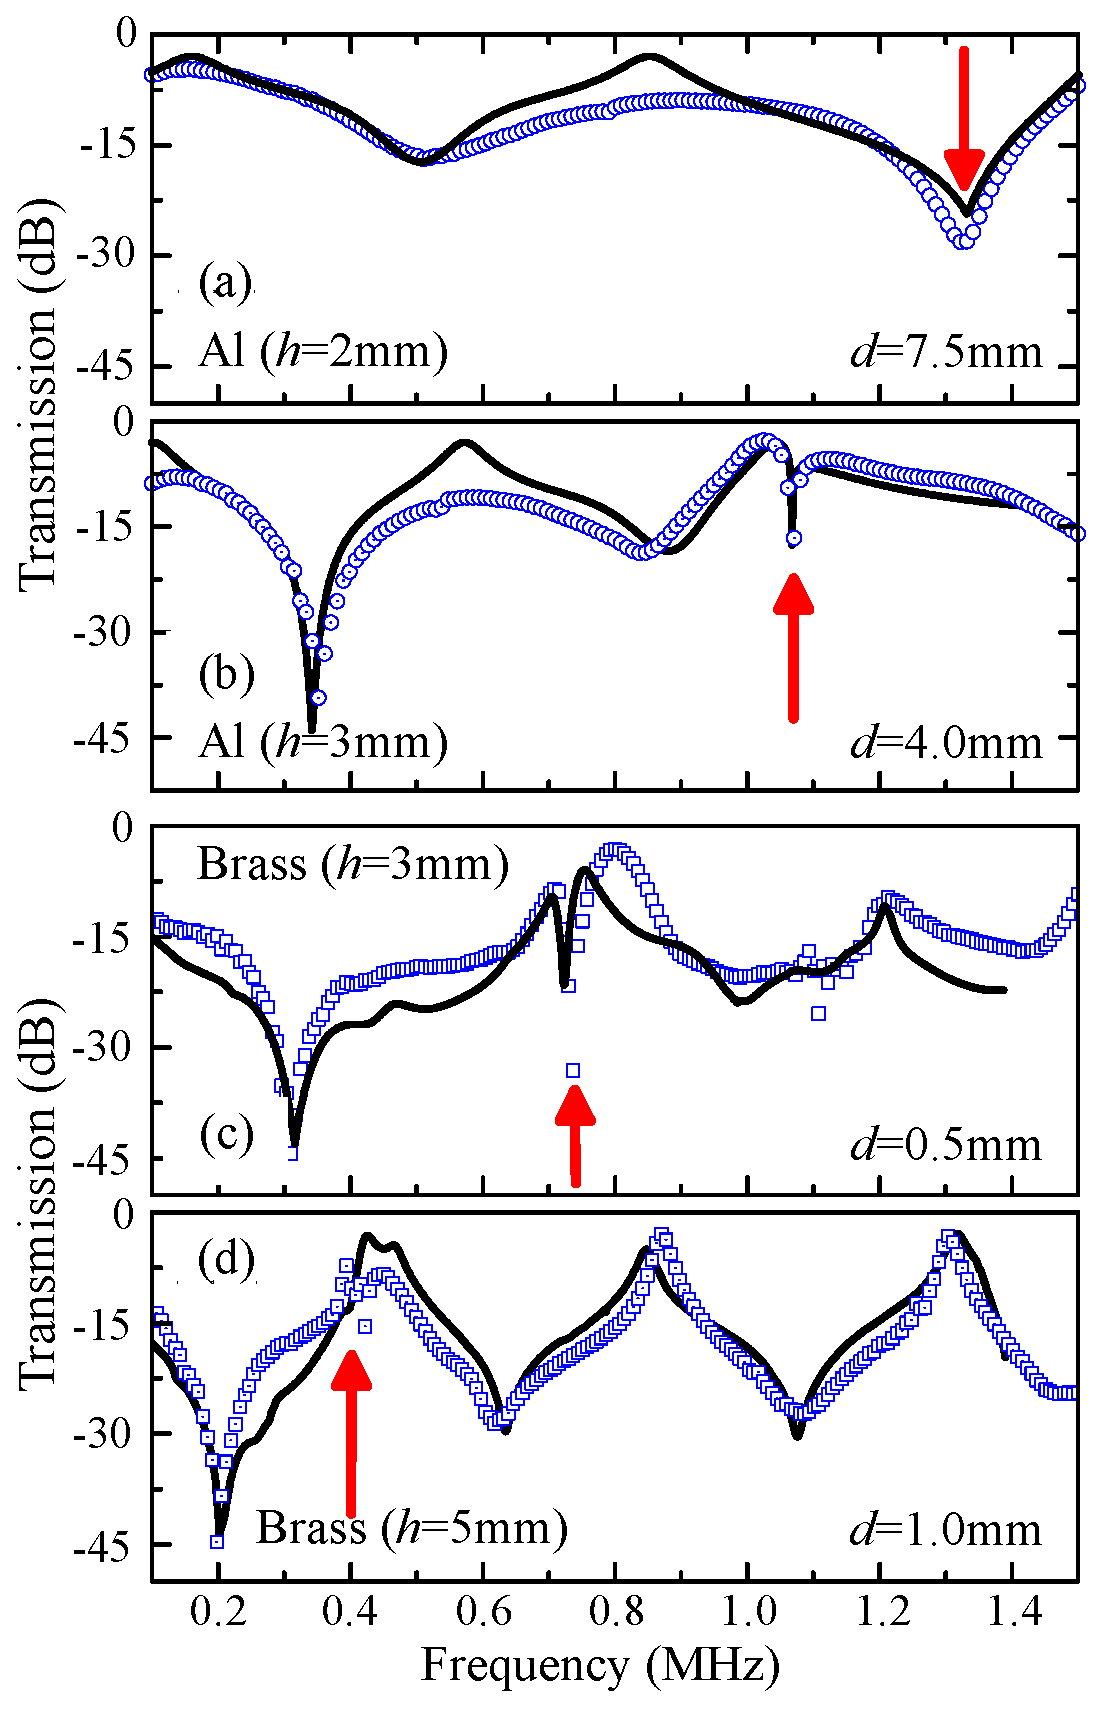
\includegraphics[width = 0.7\linewidth]{fig1_transmission_results.eps}
\caption{Sound transmission spectra of a~water slit between two aluminum (a,b) and brass (c,d) plates. Experimental results are shown by circles for aluminum and by squares for brass. Calculated spectra are shown by solid lines. The~vertical arrows mark the~minima due to the~excitation of the~slow mode.}
\label{fig:theoryexperimentRayleigh}
\end{center}
\end{figure}

\subsection{Comparison of the~Theoretical Results with the~Experiment}

In order to compare the~experimental transmission spectra \cite{channel1} with the~theoretical ones, the~transmission coefficient must be properly defined first.
The~conditions of the~experiment imply that only the~energy flux towards the~transducer surface is detected, so the~transmission coefficient should be calculated as
\begin{equation}
\label{tarn}
\mathcal{T}_{\|}(\omega) =\frac{1}{A p_0 v_{0x}} \int_A I_{x}(x=l,z) dydz
 = \frac{1}{\pi R_d^2 p_0 v_{0x}} \int_{-R_d}^{R_d} I_{x}(x=l,z) \sqrt{R_d^2-z^2} dz.
\end{equation}
Here $A=\pi R_d^2$ is the~area of the~transducer antenna, $l=8$ cm is the~$x$-coordinate of the~receiver, $p_0 v_{0x}$ is the~energy flux in the~incident wave, and 
\begin{equation}
I_{x}=p(x,z) v^{*}_x(x,z)=i \omega \rho_f T(x,z) \frac{\partial T^{\ast}(x,z)}{\partial x}
\end{equation}
is the~$x$-component of the~transmitted acoustic flux.

As shown in the~\cref{fig:theoryexperimentRayleigh}, the~theoretical spectra given by \cref{tarn} agree remarkably well with the~experimental data in a~wide frequency range for a~water ($\rho_f=1000$ kg/m$^3$, $c_f=1500$ m/s) channel.
The~fine structure of the~spectra and the~correct depth of the~minima observed at the~frequencies indicated by the~arrows are also recovered.
The~agreement is preserved when the~length and width of the~channel are varied to simulate both short and wide channels, $h < d$, \cref{fig:theoryexperimentRayleigh} (a,b), and long and narrow ones, $d < h$, \cref{fig:theoryexperimentRayleigh} (c,d), and also when the~material of the~plates is alternated between brass ($\rho_m=8400$ kg/m$^3$, $c_t=2000$ m/s, $c_l=4250$ m/s) and aluminum ($\rho_m=2700$ kg/m$^3$, $c_t=3130$ m/s, $c_l=6230$ m/s).

Indeed, as long as the~linear Hooke's law is applicable and the~viscous effects are negligible, the~calculations outlined above are guaranteed to be exact since they are based on the~exact solutions of the~wave equations.
The~stress-strain relationship is, of course, linear if the~amplitudes of the~incident wave and, consequently, of the~media vibrations are not too large.
As for the~viscous phenomena, it is known that they are manifested mainly within the~viscous layers at the~fluid-solid interfaces.
In water with the~viscosity coefficient $\nu=0.01$ cm$^2$/s these layers have a~typical thickness of approximately $\sqrt{2\mathbf{\nu}/\omega} \approx 10^{-4}$ cm in the~frequency range studied.
The~scale of the~viscous layers then appear to be several orders of magnitude smaller than the~scale of the~channel, and for that reason, the~accuracy of the~obtained results practically does not suffer if the~fluid is treated as inviscid.

The~factor that impacts the~accuracy the~most is the~number of eigenmodes that are accounted for in the~series \cref{pot1}-\cref{pot3}.
As was mentioned earlier, any propagating eigenmode that exists for a~given frequency must always be included.
On the~contrary, among the~infinite number of leaky modes choosing only the~first few in the~increasing order of their decay rates $\im\beta_n$ is sufficient.
The~actual number of leaky modes for each frequency is determined based on the~convergence of the~resulting transmission spectrum.
Naturally, the~series \cref{pot1}-\cref{pot3} converge slower for wider channels.
This is due to the~scaling $\omega_n \sim 1/d$ of the~mode eigenfrequencies.
For example, increasing the~channel width $d$ red-shifts the~cutoff frequencies \cref{eq:cutoffRayleigh} of the~propagating fast modes, so for a~wider channel a~larger number of fast modes may emerge within the~same frequency range.
In other words, the~wider the~channel the~more coupled Rayleigh modes it can support.

Specifically, the~spectra shown in \cref{fig:theoryexperimentRayleigh} (a)-(d) correspond to the~channels which support up to 8, 5, 2, and 2 propagating Rayleigh modes, respectively, in the~frequency range from 0.1 MHz to 1.4 MHz.
The~first of these modes is a~slow mode that exists for any frequency, and the~remaining fast modes start at their own cutoff frequencies \cref{eq:cutoffRayleigh}.
For the~channel of width $d=1.0$ mm between the~two brass plates, for example, the~fast mode with $n=2$ emerges at the~frequency 2.35 MHz, so obviously it cannot contribute to the~transmission below 1.4 MHz.
However, in the~twice wider channel the~same mode would appear at 1.17 MHz, and its contribution then could not be ignored.
The~number of leaky modes necessary to achieve convergence in the~cases of \cref{fig:theoryexperimentRayleigh} (a)-(d) was 11, 11, 7, and 7, respectively.
The~next leaky mode, if included in the~calculations, leads to the~variation in the~result which is considerably less than 1\%.

%The~proposed method of calculation of transmitted and reflected acoustic fields excited by a~plane wave is practically exact. The~only physical approximations we used -- the~linear Hooke's Law and inviscid fluid -- do not really affect the~accuracy of the~obtained results.  Indeed, the~width of the~viscous boundary layer $\sqrt{2 \nu/\omega} \approx 10^{-4}$ cm in water ($\nu =0.01$ cm$^2$/s) is negligible as compared with the~apertures used in our experiments. Therefore, the~calculated spectra of {\it direct} transmission
%\begin{equation}
%\label{tarn}
%\mathcal{T}_{\|}(\omega) =\frac{1}{A p_0 v_{0x}} \int_A I_{\|}(x=l,z) dydz
% = \frac{1}{\pi R_d^2 p_0 v_{0x}} \int_{-R_d}^{R_d} I_{\|}(x=l,z) \sqrt{R_d^2-z^2} dz
%\end{equation}
%are in excellent agreement with the~experimental spectra, as shown in \cref{fig:theoryexperimentRayleigh}. Here $A=\pi R_d^2$ is the~area of the~transducer antenna, $l= 8$ cm is the~coordinate of the~receiver, $p_0 v_{0x}$ is the~flux in the~incident wave, and $ I_{\|}=p(x,z) v^{*}_x(x,z)=i \omega \rho_f T(x,z) (\partial T^{\ast}(x,z)/\partial x)$ is parallel to the~channel component of the~transmitted flux of sound energy. Note that no fitting parameters were used in the~plots. The~agreement is observed within a~wide range of frequencies, for different metal plates (aluminum and brass), and for very different geometry of the~slit: short and wide channel, $h<d$, \cref{fig:theoryexperimentRayleigh} (a,b) and long and narrow channel, $d<h$, \cref{fig:theoryexperimentRayleigh} (c,d).

% The~accuracy of the~theoretical spectra depends on the~number of complex roots of \cref{disp} included in the~expansions \cref{pot}. To plot the~transmission spectra in \cref{fig:theoryexperimentRayleigh} we numerically calculated each root as a~function of frequency, i.e. each root generates a~trajectory $\xi_n(\omega)$ in the~complex $\xi$ plane (see \cref{fig:roots}).   The~convergence of the~series \cref{pot} is  slower for  wider channels, therefore in calculations of the~results shown in \cref{fig:theoryexperimentRayleigh} (a) and (b) the~number of complex roots was 11, while the~plots in \cref{fig:theoryexperimentRayleigh} (c) and (d) were obtained with only 7 complex roots.
% For all the~graphs addition of one more complex root leads to less than $1\%$ variation.
% As in any waveguide the~number of real roots (propagating modes) increases with frequency, i.e. each new real root emerges at cutoff frequency, except the~slow mode which starts from zero frequency. For the~fast mode the~cutoff frequencies $Q_n c_t/d$ are obtained from \cref{veloc}. For the~frequencies near 1.4 MHz \cref{disp} has 8, 5, 2, and 2 real roots for the~channels whose spectra are shown in \cref{fig:theoryexperimentRayleigh} (a)-(d). One of these running modes is always the~slow mode. In the~case of brass channel the~cutoff frequency for the~second ($n=1$) waveguide mode  $Q_1 c_t/d= 2.35$ MHz for the~channel with width $d=1$ mm. Therefore, it does not contribute to sound transmission in our experiments.  Its contribution becomes essential for width $d>2$ mm.

%%%%%%%%%%%%%%%%%%%%%%%%%%%%%%%%%%%%%%%%%%%%%%%%%%%%%%%%%%%%%%%%%%%%%%%%%%%%%%%%%%%%%%%%%%%%%%%%%%%%%%%%%%%%%%%%%%%%%%%%%%%%%%%%%%%%%%%%%%%%%%%%
%                                     FIGURE #3
%%%%%%%%%%%%%%%%%%%%%%%%%%%%%%%%%%%%%%%%%%%%%%%%%%%%%%%%%%%%%%%%%%%%%%%%%%%%%%%%%%%%%%%%%%%%%%%%%%%%%%%%%%%%%%%%%%%%%%%%%%%%%%%%%%%%%%%%%%%%%%%%%%%%%%%
\begin{figure}
\begin{center}
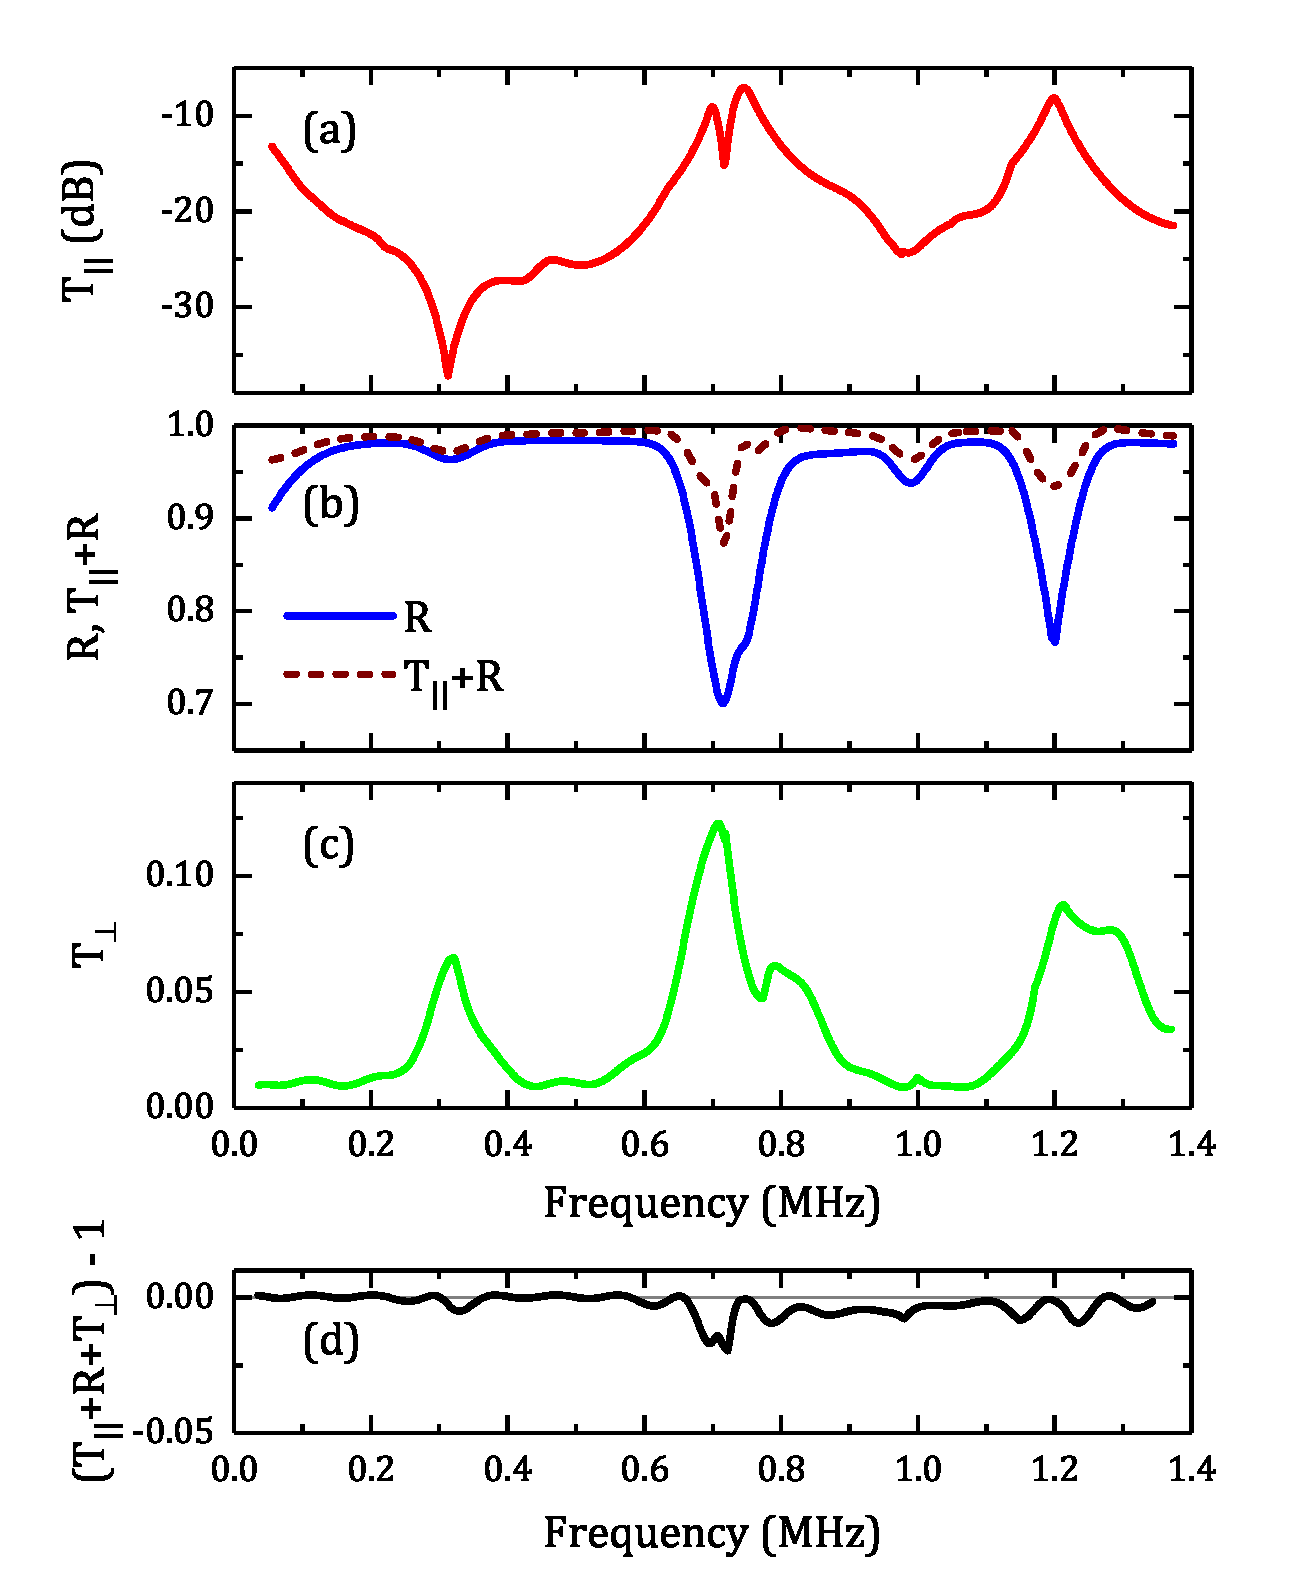
\includegraphics[width = 0.8\linewidth]{TrRe.eps}
\caption{Calculated transmission and reflection spectra for two brass plates with sides of length $L=12$ cm separated by a~channel with $h =3$ mm and $d=0.5$ mm.  (a) Transmission through the~solid vertical boundary $x = h$ (solid red line) in log scale. (b) Reflection from the~solid vertical boundary $x=0$ (blue), and the~sum $T_{\|}+R$ (brown dashed line). (c) Transmission through the~horizontal boundary $z = d/2$. (d) The~conservation of energy as demonstrated by the~sum $T_{\|}+T_{\perp}+R$, which does not deviate from 1 by more than $2\%$.}
\label{fig:fig3}
\end{center}
\end{figure}

\subsection{Redirection of Sound into Elastic Plates}

Additional insights into the~physical reasons for the~extraordinary low transmission in \cref{fig:theoryexperimentRayleigh} can be gained by the~examination of how the~acoustic energy is scattered in the~system.
For the~water channel with $h=3$ mm and $d=0.5$ mm with the~spectrum shown in \cref{fig:theoryexperimentRayleigh}(c) I calculate both the~transmission and the~reflection spectra.
These two coefficients are redefined here in order to account for the~total flux in the~$x$-direction through the~entire solid boundaries $x=0$ and $x=h$:
\begin{equation}
T_{\|} = 2\frac{i \omega \rho_f^2 c_f }{p_0^2 L} \int_{d/2}^{\infty} T(h,z)\left.\frac{\partial T^{*}(x,z)}{\partial x}\right|_{x=h}\, dz,
\end{equation}
\begin{equation}
R = -2\frac{i \omega \rho_f^2 c_f }{p_0^2 L} \int_{d/2}^{\infty} R(0,z)\left.\frac{\partial R^{*}(x,z)}{\partial x}\right|_{x=0}\, dz.
\end{equation}
Also, I calculate the~flux that is transmitted from the~water channel into the~plates through the~boundaries $z=\pm d/2$:
\begin{equation}
T_{\perp} = 2\frac{i \omega \rho_f^2 c_f }{p_0^2 L} \int_{0}^{h} B(x,z)\left.\left(\frac{\partial B^{*}(x,z)}{\partial z}\right)\right|_{z=\frac{d}{2}}\, dx.
\end{equation}

The~three curves are shown in \cref{fig:fig3}.
Interestingly, at the~frequencies where the~minima in transmission are observed the~reflection is also suppressed (see \cref{fig:fig3} (b)).
Calculation of the~sum of the~fluxes exiting from either vertical side of the~plate reveals that there must be an~additional energy supplied to the~plates as the~sum $T_{\|}+R$ falls considerably below 1 for a~wide range of frequencies.
Clearly, this additional portion of energy has to be coming from the~fluid channel through the~channel walls.
The~spectrum of this vertical flux, $T_{\perp}$, is shown in \cref{fig:fig3} (c).
The~minima of $T_{\|}$ and $R$ coincide with the~maxima of $T_{\perp}$, and the~total flux that goes through the~sides of the~plates is very close to 1 which is expected as the~total energy must be conserved in the~system (see \cref{fig:fig3} (d)).
The~flux through the~other end of the~plate, at $z=\infty$, is negligible as all of the~leaky Rayleigh modes carrying energy will necessarily be scattered through the~vertical sides in a~sufficiently long plate.
The~minor fluctuations of $T_{\|}+R+T_{\perp}$ around 1 are due to the~numerical error that builds up during the~calculations.
The~analysis performed here stresses that the~channel system cannot be regarded as an~aligned along $z$-axis 1D scatterer of acoustic waves.

The~elastic nature of plates in the~2D system studied allows for an~interesting ability to redirect the~acoustic excitation into the~plates.
The~waves in the~plates may then propagate perpendicular to the~direction of the~incident wave.
This feature can not be described in the~models employing the~rigid-body approximation which is quite commonly used in a~great number of acoustic studies.
Therefore, only the~elastic screens have the~capability to redirect sound into metal at an~almost $90^o$ angle.
The~redirected flux can be observed to be as high as 12\%, as can be seen from \cref{fig:fig3} (c) for the~frequency of around 0.7 MHz.
This is quite a~strong effect, and the~amount of redirected flux can be comparable with the~flux transmitted through a~brass plate in water (as low as 8\%, or $-11$ dB, for the~frequency of the~Fabry-Perot minimum).

%In order to analyze physical nature of the~deep minima in \cref{fig:theoryexperimentRayleigh}, we calculated the~reflection spectrum for the~slit with $h=3$mm and $d=0.5$ mm and plotted it in \cref{fig:fig3} together with the~total transmission $T_{\|}$ through the~whole boundary $x=h$.

%The~positions of the~minima in the~reflection in \cref{fig:fig3} (a) coincides with the~positions of the~minima in the~transmission in \cref{fig:theoryexperimentRayleigh} (c).  Near these minima the~sum of forward and backward scattered flux, $T_{\|}+R$, is considerably less than 1, that is a~clear indication that this sum does not represent the~total flux scattered by the~slit. Since the~slit shown in \cref{fig:theoryexperimentRayleigh} is a~2D scattering system,  the~lack of scattered flux, $1-T_{\|}-R$, is the~energy scattered along axis $z$.
%In \cref{fig:fig3}b we plot the~spectrum transmitted from the~fluid to the~metal through the~horizontal boundary $z=d/2$.
%It exhibits maxima exactly at the~frequencies where $T_{\|}+R$ exhibits minima, thus representing the~flux, $T_{\perp}$, which is lost if the~slit is approximated as a~1D scatterer.
%The~total scattered flux $T_{\|}+T_{\perp}+R$, while fluctuates due to numerical errors, still remains very close to 1, as it is shown in the~inset to \cref{fig:fig3}b.

%Vibrations of the~metal-fluid boundary $z=\pm d/2$ break 1D symmetry of the~system, {\bf i.e. these boundaries are not flat any more.  This broken symmetry} gives rise to the~elastic wave propagating in the~metal plates perpendicular to the~incident wave.  The~flux of energy $T_{\perp}$ associated with this redirected wave does not appear in the~model of rigid screen which was accepted in many previous studies. Therefore, the~property of a~slit to redirect the~incoming flux into metal is manifested only for elastic screens. The~amount of redirected acoustic energy may reach $12\%$ at the~frequencies near 0.7 MHz, as shown in \cref{fig:fig3}. This is relatively strong effect, taking into account that a~brass plate in water transmits only about $8\%$ (-11 Db) in the~minimum of the~Fabry-Perot resonance. 

%%%%%%%%%%%%%%%%%%%%%%%%%%%%%%%%%%%%%%%%%%%%%%%%%%%%%%%%%%%%%%%%%%%%%%%%%%%%%%%%%%%%%%%%%%%%%%%%%%%%%%%%%%%%%%%%%%%%%%%%%%%%%%%%%%%%%%%%%%%%%%%%%%%%%%%%%%%%%
%                                                               FIGURE #4
%%%%%%%%%%%%%%%%%%%%%%%%%%%%%%%%%%%%%%%%%%%%%%%%%%%%%%%%%%%%%%%%%%%%%%%%%%%%%%%%%%%%%%%%%%%%%%%%%%%%%%%%%%%%%%%%%%%%%%%%%%%%%%%%%%%%%%%%%%%%%%%%%%%%%%%%%%%%%
%
\begin{figure}
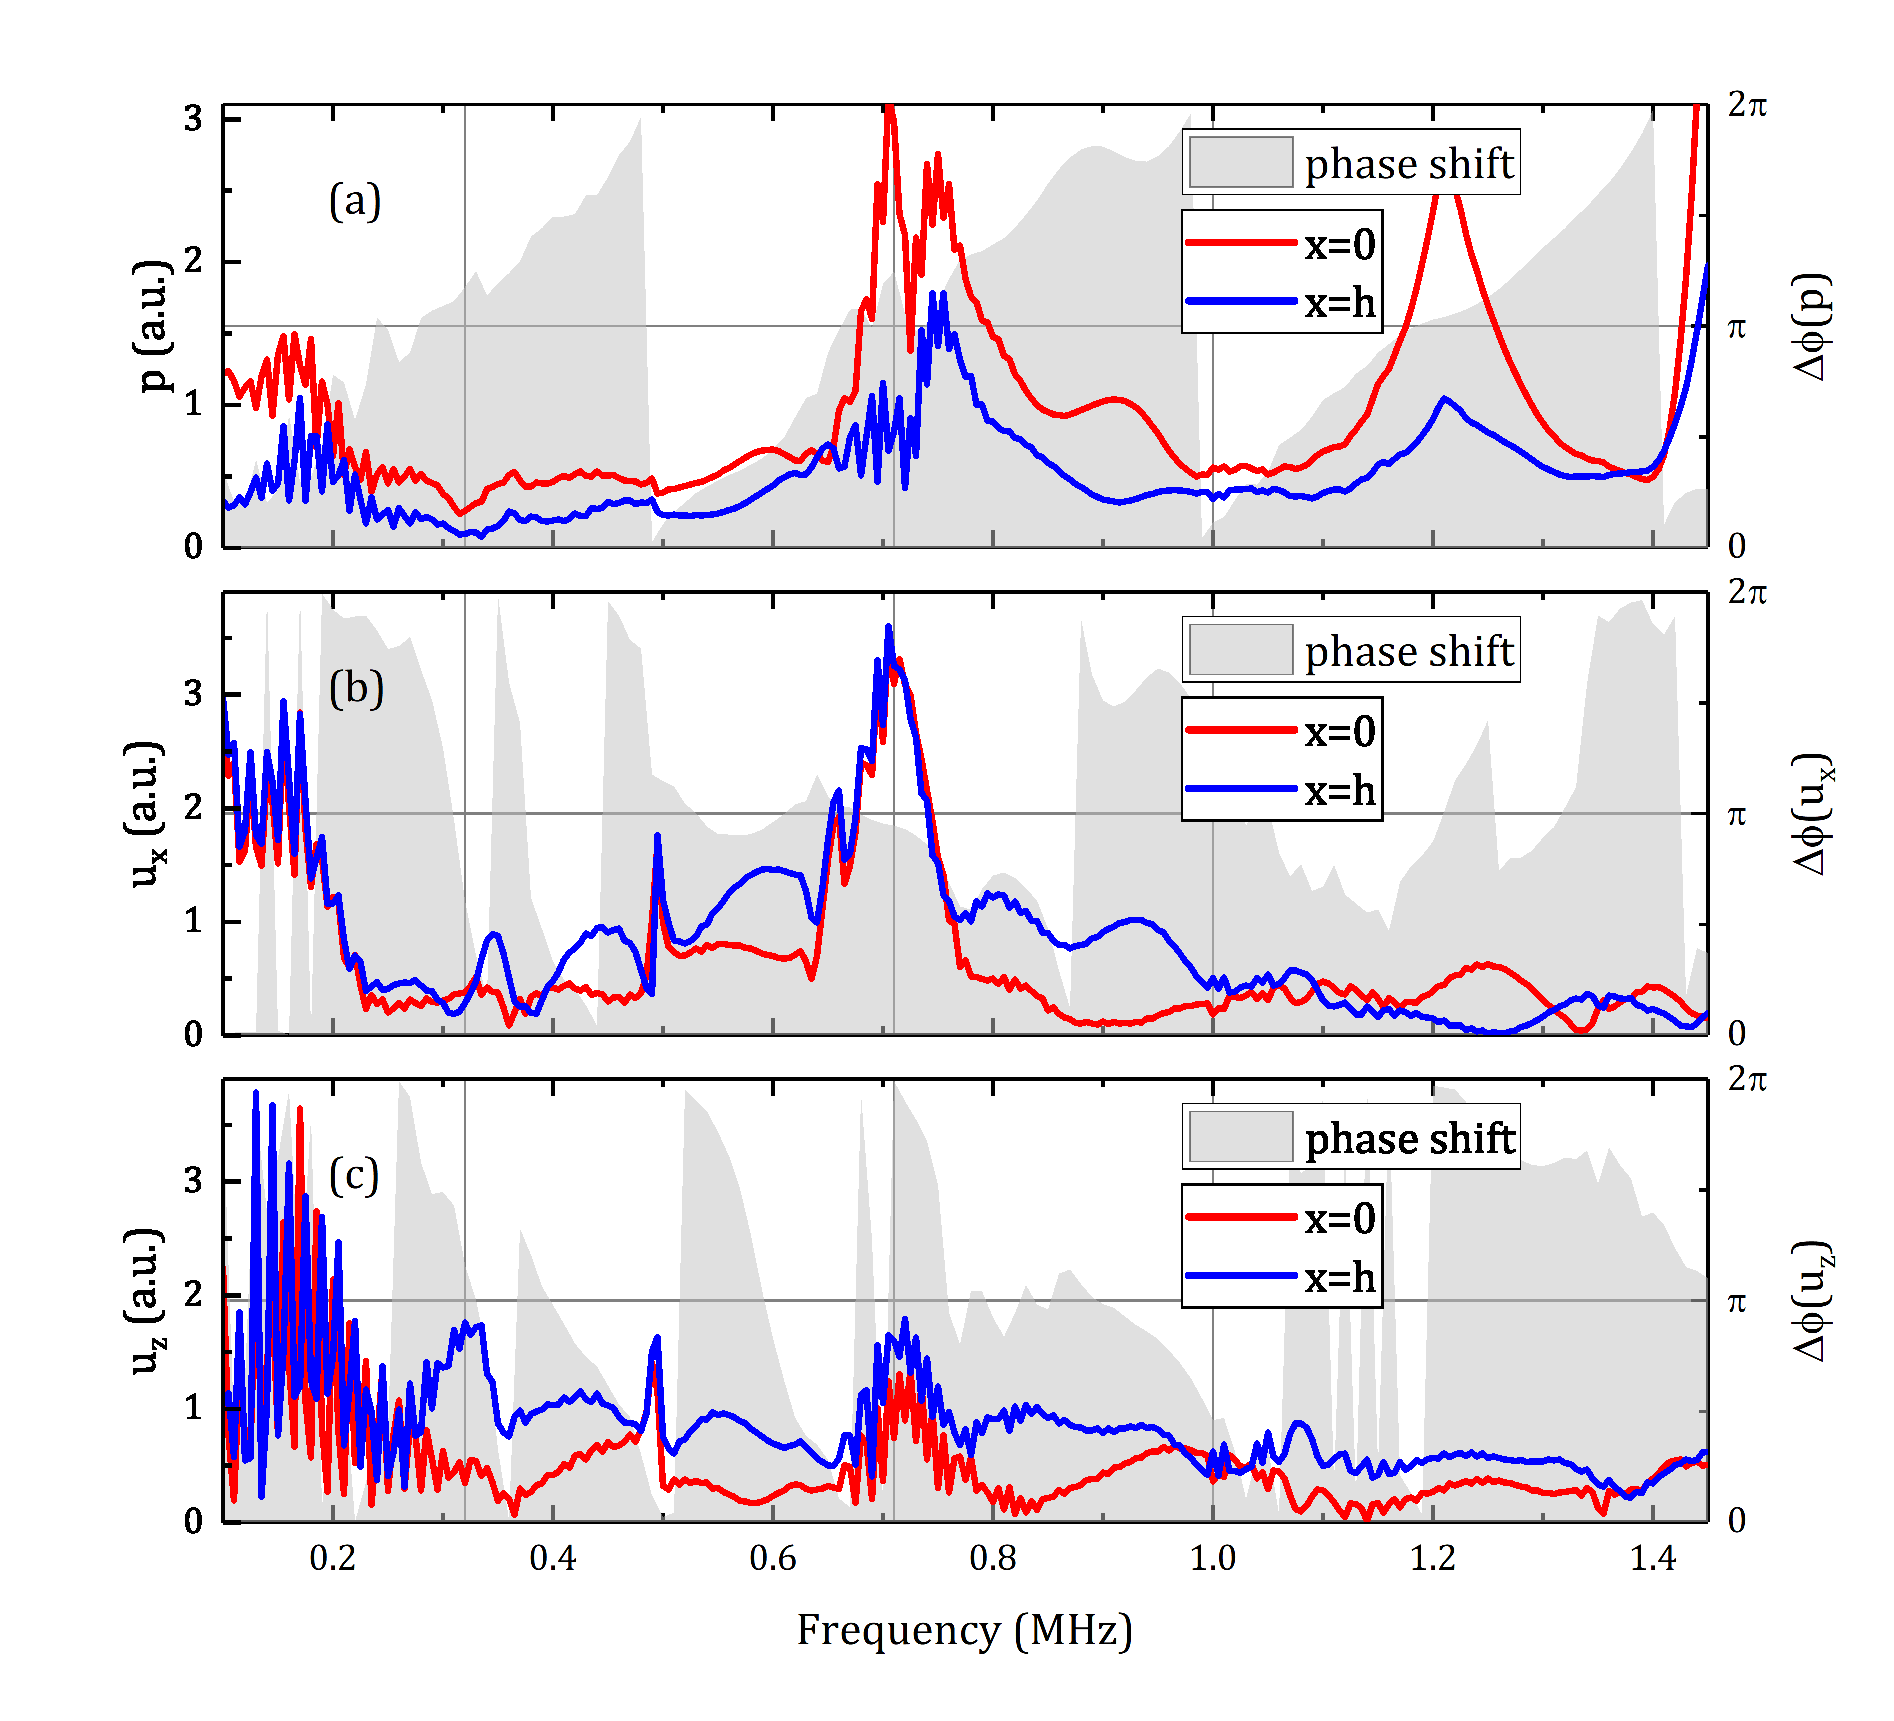
\includegraphics[width=0.9\linewidth]{p_ux_uz.eps}
\caption{Frequency dependence of the~pressure, $x$ and $z$ displacement of the~plates at the~left and right ends of the~same channel as in \cref{fig:fig3}. The~solid curves show the~amplitude of the~respective quantity calculated at the~points $x=0$ (red) and $x=h$ (blue). The~shaded regions represent the~phase shifts $\Delta\phi(g)=\arg \left.g\right|_{x=0}-\arg \left.g\right|_{x=h}$ for each quantity $g=p,u_x,u_z$ whose amplitudes are plotted in the~same panel. Straight vertical lines mark the~positions of the~deep minima in the~transmission shown in \cref{fig:theoryexperimentRayleigh} (c).}
\label{fig:fig4}
\end{figure}


In order to understand how individual Rayleigh eigenmodes enhance the~radiation of energy into the~plates, I analyze frequency dependence of the~pressure and both $x$- and $z$-components of the~displacement vector evaluated at the~corners of the~channel ($x=0,h$, and $z=d/2$).
The~respective graphs are visualized in \cref{fig:fig4}.
Each panel of the~figure is dedicated to a~certain physical quantity.
The~solid lines show the~amplitudes of that quantity for either corner of the~channel as a~function of frequency, and the~shaded area gives the~relative phase shift between the~two.

For the~resonant frequencies that correspond to the~minima in transmission (0.32 MHz, 0.71 MHz, and 0.98 MHz) the~horizontal displacement appears to have very small amplitudes close to the~first and third resonances (which are basically the~Fabry-Perot minima).
In the~second resonance the~amplitudes are quite large, and the~phase shift is close to $\pi$, meaning the~vibrations are out of phase.
This corresponds to high transmission of sound, so the~appearance of the~dip must be caused by another factor.
Namely, the~pressure at both ends of the~channel in the~resonances is close to zero or exhibits a~sharp dip.
As for the~vertical displacement, its contribution to the~redirection of sound is due either to the~amplitudes at each corner being close and in phase (close to $0$ or $2\pi$), or one amplitude being much larger than the~other.

Both the~suppressed direct transmission and the~suppressed reflection are necessary conditions to have the~strong redirection of flux into the~metal plates.
This requires having simultaneously low pressure $p(x,z)$ and small amplitudes of horizontal vibrations $u_x(x,z)$ of the~plate boundaries at the~channel ends.
Naturally, when the~pressure minima occur at the~same (or very close) frequencies as the~displacement minima, the~extraordinary low transmission of sound ensues.
The~sharpness of the~dip in \cref{fig:theoryexperimentRayleigh} correlates with the~amount of energy being redirected.
The~closer the~frequencies for which both $p$ and $u_x$ are low, and the~closer these quantities are to zero, the~sharper becomes the~dip, and, consequently, the~more energy veers into the~metal.
Moreover, it helps to have the~local maxima for the~$z$-component of the~displacement at the~resonant frequency to facilitate the~redirection of energy into the~metal.
While the~frequency dependence on every individual panel in \cref{fig:fig4} exhibits the~described behavior for multiple frequencies, the~effect builds up when this behavior is manifested simultaneously, i.e., at the~same frequency.
For example, the~third resonance is much broader than the~other due to quite weak vertical oscillations of the~plate boundaries.

Qualitatively, one can conclude about the~strength of the~effect based on how different eigenmodes propagating in opposite directions in the~channel interfere to form standing (or, better to say, quasi-standing) waves across the~length of the~channel $h$.
Indeed, since the~propagating Rayleigh eigenmodes exhibit usual oscillating behavior along the~$x$-axis, the~low pressure at the~channel ends occurs when the~modes interfere destructively.
Specifically, the~most suppression of transmission results from the~destructive interference of the~eigenmode which would otherwise contribute the~most to the~transmission.
If at the~same frequency another eigenmode interferes destructively as well, the~dip in the~spectrum becomes even sharper.
Even though it is possible to conclude how the~modes interfere, it is, nevertheless, quite challenging to determine how much energy is redirected as a~function of the~channel geometry since it explicitly depends on the~dispersion \cref{eq:dispersionXiRayleigh} of each involved Rayleigh eigenmode.

The~two principal maxima in transmission, at 0.71 MHz and 1.22 MHz, are the~maxima of the~Fabry-Perot resonances, and they simply coincide with the~minima in the~reflection spectrum.
Also, the~amplitude of the~transmitted pressure is quite large (see \cref{fig:fig4}(a)).
Since these Fabry-Perot maxima result from the~constructive interference of the~quasi-longitudinal leaky Rayleigh mode, their positions are strongly affected by the~mode dispersion.
The~Fabry-Perot resonances of the~bulk metal plate are equidistant in the~frequency spectrum, where as for the~system with the~channel the~maxima get closer to each other for higher frequencies.
This is due to the~phase speed of the~quasi-longitudinal mode decreasing with frequency, as shown in \cref{fig:roots}.

In \cref{fig:theoryexperimentRayleigh}(c) the~two minima in transmission at 0.32 MHz and 0.71 MHz in transmission arise due to the~constructive interference of the~propagating eigenmodes with the~phase speeds $\xi_1 = 0.99$ and $\xi_2 = 0.715$, respectively.
The~mode responsible for the~minimum at 0.32 MHz is a~fast mode that could be excited only above its cutoff frequency of about 0.3 MHz.
Its phase velocity is greater than the~speed of sound in water, $c=c_t\xi_1 > c_f$.
This minimum coincides with the~Fabry-Perot maximum, thus producing an~asymmetric fine structure in the~transmission spectrum.

The~second minimum is created by a~slow mode, which propagates slower than the~pressure wave in water.
Both minima caused by the~respective eigenmodes are quite sharp due to the~suppression of the~principal mode that is responsible of transmitting the~most energy through the~channel.


%\subsection{Verification by FEM Modeling}
The~results described above were independently verified by simulating the~transmission of sound using the~finite element method (FEM) \cite{channel2}. %with the~COMSOL Multiphysics\textsuperscript{\textregistered} software .
The~simulated spectra provided the~agreement with both the~theory and the~experiment and illustrated how the~elastic waves initially localized near the~channel walls are transformed into the~leaky waves as they propagate in the~channel.
The~viscous effects were omitted in the~simulations, which confirmed that the~observed transmission features are not due to the~unaccounted dissipation in water.

%\textcolor{red}{add here}

%The~first root corresponds to excitation of the~ fast mode, since its phase velocity $c_t \xi_1$ exceeds the~speed of sound in the~fluid $c_f$. For the~second root, $\xi_2$, the~phase velocity of the~corresponding eigenmode is less than $c_f$, therefore this minimum is due to excitation of the~slow mode.
%The~minima associated with excitation of the~slow mode are marked by arrows in the~transmission spectra shown in \cref{fig:theoryexperimentRayleigh}.
%As a~rule, these minima are sharp and asymmetric, except the~minimum at 0.4 MHz in \cref{fig:theoryexperimentRayleigh} (d), which structure is strongly affected by a~standard Fabry-Perot resonance.

%Enhanced radiation of sound into metal occurs due to large amplitude of vertical vibrations $u_z$ of the~plate boundaries at $z= \pm d/2$. Suppressed direct transmission and reflection originate from low pressure $p(x,z)$ at the~channel ends and also from small amplitude of horizontal vibrations $u_x$ of the~plate boundaries $x= 0$ and $x=h$. When these two effects occur at close frequencies they mutually enhance each other, leading to extraordinary low transmission. {\bf The~sharper a~dip in \cref{fig:theoryexperimentRayleigh}, the~more energy is redirected into metal. The~sharpness of a~dip depends on how close to zero the~pressure $p(x,z)$ and the~displacement $u_x$ become at $x= 0,h$. Being represented by  a~sum of plane waves taken over the~roots of the~dispersion equation, these quantities become small when those plane waves that give the~principal contribution interfere almost destructively at the~length of the~channel $h$. It may accidentally occur that two plane waves with \textit{smaller} amplitudes also interfere destructively, thus leading to even sharper dip. It is, however, \textit{nearly} impossible to predict how the~amount of redirected energy depends on the~geometry of the~channel and frequency, since it depends on the~values of real roots of the~transcendental equation \cref{disp}.


%In \cref{fig:fig4} we plot the~pressure and the~ amplitudes of horizontal and vertical vibrations at the~channel ends ($x = 0,h$) vs frequency. It is clearly seen that near the~resonant frequencies where minima in the~transmission are experimentally observed (marked by vertical lines) the~amplitude of horizontal vibrations of the~both faces of the~plates is close to zero.  The~same is true for the~pressure at the~ends of the~channel. Since the~vibrations of the~plates and the~fluid are coupled through the~boundary conditions, we conclude that a~quasi-standing wave is formed in the~whole system due to interference between two eigenmodes propagating in opposite directions.
%At the~same resonant frequencies the~amplitude of the~vertical vibrations reaches its local maxima that explains strong radiation into metal. While the~graphs in \cref{fig:fig4} exhibit many peaks, strong redirection of sound occurs when minimum in pressure and displacement $u_x$ coincides with maximum in displacement $u_z$. The~depth and width of the~minimum in $T_{\|}$ depends on how close to each other these three extrema occur. For example, the~first two minima at 0.32 and 0.71 MHz in Figs. \cref{fig:theoryexperimentRayleigh} (c) and \cref{fig:fig3} (a) are well pronounced since the~frequencies of all three extrema practically coincide. Unlike this, the~third minimum at 1 MHz is quite broad due to visible shifts in the~positions of the~extrema.
%There are two Fabry-Perot resonances at 0.72 and 1.22 MHz in the~transmission spectrum in \cref{fig:theoryexperimentRayleigh} (c). Here the~situation is quite simple and standard --  maximum in transmission coincides with minimum in reflection.
%This also can be seen from \cref{fig:fig4} (b) where the~amplitude of longitudinal vibrations at the~right face ($x=h$) of the~plate exceeds that on the~left face ($x=0$), especially for the~resonance at 1.22 MHz which is not affected by close proximity of a~deep minimum in transmission. 

%In \cref{fig:theoryexperimentRayleigh} (c) two minima at 0.32 and 0.71 MHz in transmission are associated with appearance of the~real roots of \cref{disp}, $\xi_1 = 0.99$ and $\xi_2 = 0.715$, respectively. The~first root corresponds to excitation of the~ fast mode, since its phase velocity $c_t \xi_1$ exceeds the~speed of sound in the~fluid $c_f$. For the~second root, $\xi_2$, the~phase velocity of the~corresponding eigenmode is less than $c_f$, therefore this minimum is due to excitation of the~slow mode.
%The~minima associated with excitation of the~slow mode are marked by arrows in the~transmission spectra shown in \cref{fig:theoryexperimentRayleigh}.
%As a~rule, these minima are sharp and asymmetric, except the~minimum at 0.4 MHz in \cref{fig:theoryexperimentRayleigh} (d), which structure is strongly affected by a~standard Fabry-Perot resonance.





%++++++++++++++++++++++++++++++++++++++++++++++++++++
%\section{FEM Numerical Modeling}
%++++++++++++++++++++++++++++++++++++++++++++++++++++

%\begin{figure}
%\begin{center}
%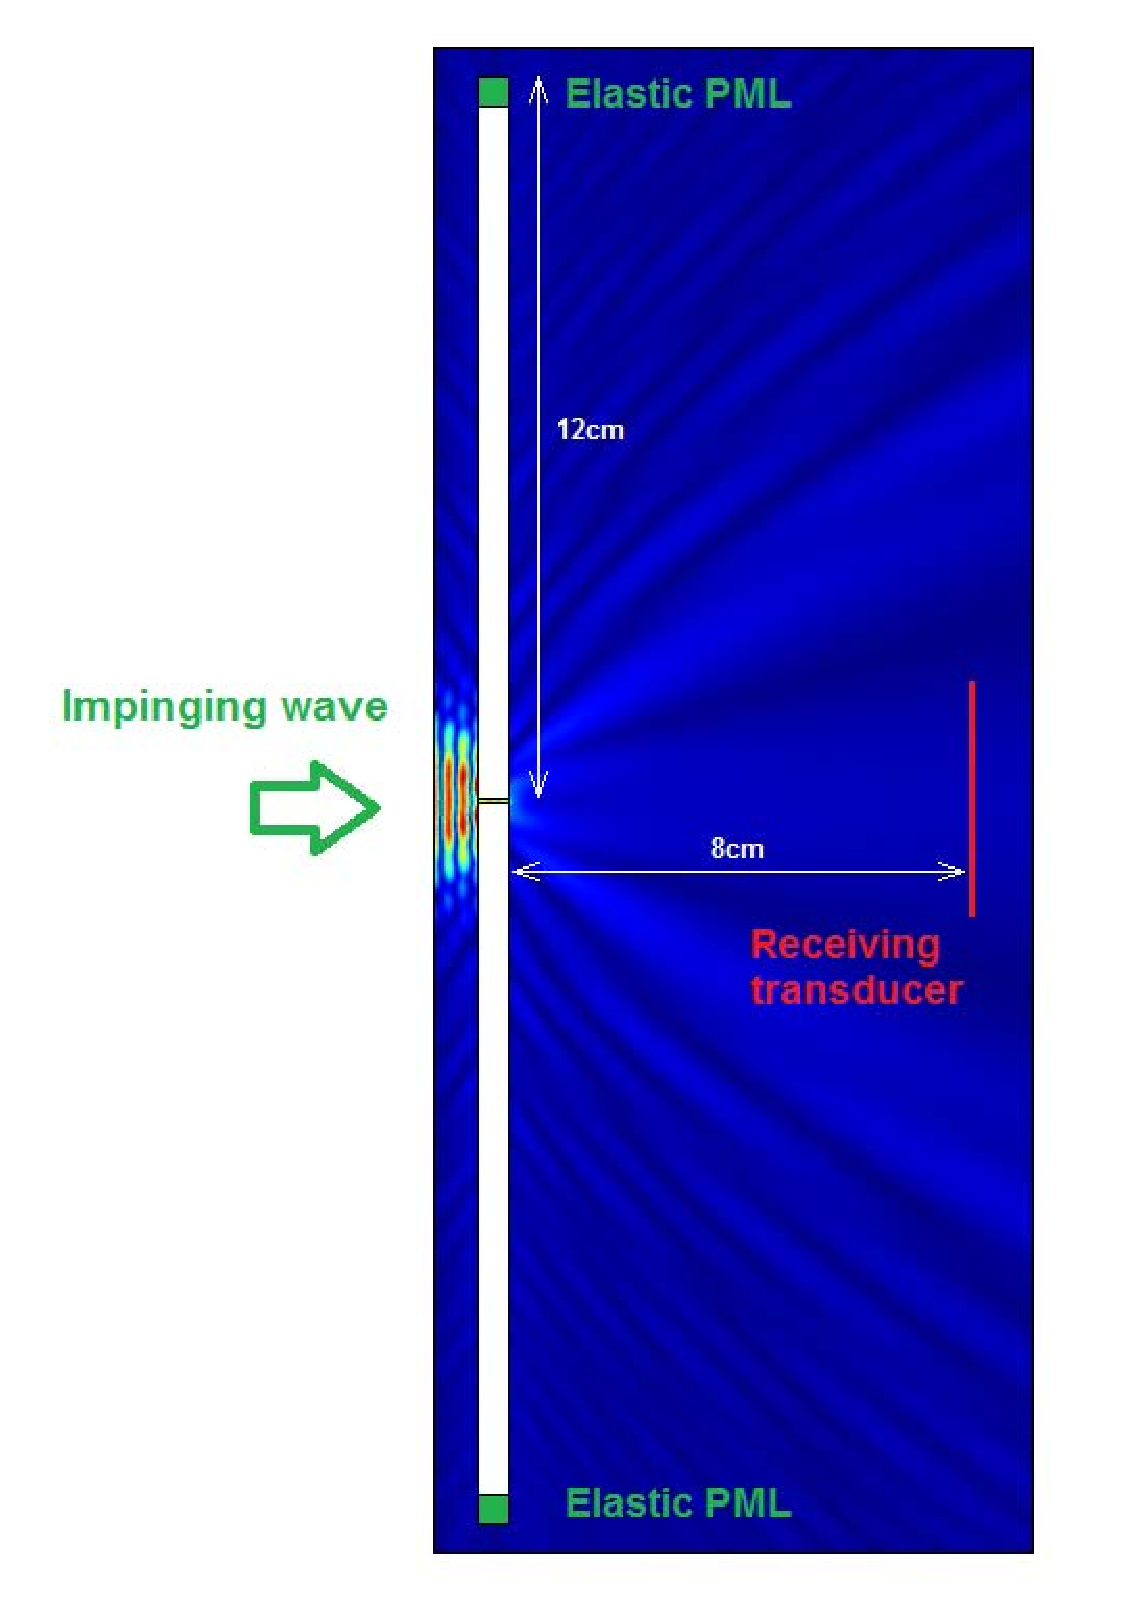
\includegraphics[width = 0.5\linewidth]{figS1.eps}
%\caption{ The~structure of the~fluid channel used for numerical simulations. A~Gaussian beam coming from the~left is incident on the~channel and the~pressure field is calculated behind the~plates. The~illustrated pattern corresponds to two brass plates with $h=5$ mm, $d=1$ mm at the~frequency 0.32 MHz.}
%\label{fig:fig5}
%\end{center}
%\end{figure}

%\begin{figure}
%\begin{center}
%\includegraphics[width = \linewidth]{figS2.eps}
%\caption{ Transmitted pressure at the~receiving antenna (in dB) for a~slit between two brass plates with $h=3$ mm (top) and $h=5$ mm (bottom) at several apertures and frequencies. Left (right) panels correspond to experimental (simulated) data.}
%\label{fig:fig6}
%\end{center}
%\end{figure}
%
%The~obtained results are additionally verified by simulating the~transmission of sound using the~finite element method (FEM).
%The~simulation was performed using the~COMSOL Multiphysics\textsuperscript{\textregistered} software, and the~geometry is shown in \cref{fig:fig5}.
%In the~model, the~two elastic plates of thickness $h$ were placed inside the~2D inviscid water domain at a~distance $d$ from each other.
%To closely match the~conditions of the~experiment, the~plates were modeled having the~same length $L=12$ cm in the~$z$ direction.
%\textcolor{red}{PMLs???}
%The~acoustic wave generated by the~transducer on the~left was approximated by a~Gaussian beam of similar effective cross section.
%The~water domain is modeled as infinite one, which is realized by imposing non-reflecting boundary conditions on the~domain's limiting borders.
%The~transmission is calculated by integrating the~sound intensity over the~vertical line of length $2R_d$ at a~distance $l=8$ cm from the~plates, which imitates the~surface of the~receiving transducer.
%The~transducer itself is not physically present in the~model.
%
%The~transmission spectra were calculated in the~frequency range from 0 to 1 MHz, with an~additional parameter sweep for the~channel width $d$ from 0 to 7.5 mm.
%The~parameters of brass were used for the~elastic properties of the~plates, and their thickness was either 3 or 5 mm.
%The~resulting data is represented by color maps in \cref{fig:fig6} on the~right panels, where the~transmission is plotted as a~function of frequency and channel aperture.
%The~left panels show the~experimental measurements, which were performed by an~automated setup for the~same parameter ranges.
%
%\textcolor{red}{change below}
%Theoretical and experimental results are also supported by finite element simulations, which were performed through the~commercially available software COMSOL Multiphysics. The~employed model is represented in \cref{fig:fig5}. It consists of a~two-dimensional domain filled with a~fluid having the~acoustic properties of water. Two elastic plates with thickness $h$ and separated by a~distance $d$ are displaced forming a
%fluid channel. The~plates are of the~same length of 12 cm as the~experimental samples.  At the~ends the~both plates terminate with two additional absorbing domains (or elastic perfectly matched layers, PML) in order to suppress reflection. Normally incident Gaussian beam is used as impinging wave to provide a~more realistic excitation. The~exterior boundaries of the~model are configured with non-reflecting conditions, ensuring that outgoing waves leave the~domain.

%A~frequency sweep is performed numerically for different thicknesses $h$ and apertures $d$ of the~slit. This process provides a~large amount of data which can be summarized through maps showing the~transmitted pressure as a~function of frequency and aperture. In addition, the~same sweep was also experimentally carried out using an~automated setup. In \cref{fig:fig6} we compare experimental and numerical data for brass plates with thickness $h=3$ mm and $h=5$ mm.
%The~numerical data are obtained by integrating the~pressure field over the~length of the~receiving transducer (see \cref{fig:fig5}).

%Both maps exhibit regions of parameters with anomalously low transmission. There is excellent agreement between the~positions of the~deep minima obtained experimentally, theoretically, and numerically. The~deepest minima  at 0.32 MHz for $h=3$ mm and at 0.2 and 0.64 MHz for $h=5$ mm appear as bright blue spots in the~maps in \cref{fig:fig6}.
%Unlike this, less deeper minima at 0.71 MHz ($h = 3$ mm) and at 0.4 MHz ($h=5$ mm) appear as narrow yellow lines on red background. This occurs because these local minima are close to the~maxima of the~Fabry-Perot resonances. These less-deeper minima correspond, as it is explained in the~main text, to excitation of the~slow mode. The~minimum at 0.4 MHz ($h=5$ mm) has a~doublet structure (see \cref{fig:theoryexperimentRayleigh}d), which is well-reproduced in the~experimental map in \cref{fig:fig6}.
%It, however, is not resolved in our numerical simulations.
%It is worth mentioning that no viscosity effects were considered in the~fluid, thus demonstrating that the~reported effects are not due to viscous phenomena inside the~channel.
%
%The~elastic displacements were also obtained from the~simulations, allowing the~observation of the~wave phenomena occurring inside the~plates.
%A~motion picture showing the~pressure map in the~fluid superimposed with the~lines of displacement (either in water or metal) is presented in the~Supplementary Material Movie S1 \cite{supp}.
%It is calculated for brass plates with $h=3$mm and $d=0.5$mm (the~same parameters as in \cref{fig:theoryexperimentRayleigh}c) at 0.704 MHz.
%It is shown how the~incoming wave generates elastic vibrations inside the~slit and the~plates and how these vibrations propagate. It is easy to see that that the~vibrations of the~plate which originally are localized near the~channel boundaries become leaky modes, carrying the~acoustic energy away from the~channel in a~form of vortices. The~vortex structure of the~displacement field in metal is due to non-potential contribution $\nabla \times S$ to the~displacement field $\bf u$. This  movie visualizes the~effect of redirection of sound by a~straight fluid channel with elastic boundaries.



%%%%%%%%%%%%%%%%%%%%%%%%%%%%%%%%%%%%%%%%%%%%%%%%%%%%%%%%%%%%%%%%%%%%
\section{Summary}
A~comprehensive study of sound transmission through a~fluid channel surrounded by elastic regions is presented in this chapter.
The~rigorous analytical solution of the~scattering problem allows to calculate the~transmission spectrum that almost coincides with the~experimental transmission data.
It is theoretically discovered that the~system exhibits an~unusual behavior --- the~behavior of a~redirecting acoustic antenna.
The~ability of the~fluid channel to redirect the~acoustic energy at an~almost $90^o$ angle into the~surrounding elastic media is quite strong, allowing to affect up to approximately 10\% of the~incoming flux.
The~phenomenon discussed above was previously unknown for the~fluid channels, and it is explained in terms of the~mutually interfering coupled Rayleigh eigenmodes of the~channel.
Simply put, whenever the~vibrations of the~fluid and the~elastic media become synchronized and form one or several quasi-standing waves in the~system, the~transmission forward and the~reflection backward are suppressed and the~acoustic flux escapes in the~remaining unusual direction.

The~analytical approach developed for this problem employs the~method of expanding the~acoustic fields over the~set of eigenmodes of the~system.
The~lack of orthogonality of the~eigenmodes does not allow for the~completely analytical solution, nevertheless, the~obtained numerical solution is  practically exact.
This approach can be applied to other problems with more complicated geometries, such as elastic screens with periodically arranged apertures.

The~effect of the~redirection of sound is important for designing of the~acoustic devices that are able to manipulate the~propagation of sound, such as acoustic waveguides or acoustic antennas.

%In summary, we reported a~comprehensive study of sound transmission through a~finite-length fluid channel with elastic boundaries. It is experimentally observed and explained and how a~straight fluid slit between two metallic screens may serve as a~redirecting acoustic antenna.
%This previously unknown property is due to excitation and interference of the~eigenmodes which describe the~synchronized vibrations of the~fluid and metal plates.
%Maximum of energy redirected into the~plates occurs when \textbf{as many eigenmodes as possible become quasi-standing waves on the~length of the~channel simultaneously}.
%The~proposed method of solution of the~scattering problem for a~slit is practically exact and leads to excellent agreement with the~experiment. The~proposed analytical approach may be easily extended to more complicated geometries, in particular, to a~set of periodically arranged slits.
%The~effect of redirection of sound may find applications in design of specific devices for  manipulation of acoustic energy and vibration of plates embedded into fluids. The~resonant modes which are responsible for the~redirection of sound are of particular interest for microfluidics since pressure produced by the~vibrating boundaries is comparable with the~capillarity force or the~force generated by a~micropump.






%%% Local Variables: 
%%% mode: latex
%%% TeX-master: "dissertation"
%%% End: 

%%%%%%%%%%%%%%%%%%%%%%%%%%%%%%%%%%%%%%
\chapter{REDIRECTION OF SOUND BY A PERIODIC CHAIN OF PERFORATED METALLIC CYLINDRICAL SHELLS}
%%%%%%%%%%%%%%%%%%%%%%%%%%%%%%%%%%%%%%

%%%%%%%%%%%%%%%%%%%%%%%%%%%%%%%%%%%%%%%%%%%%%%%%%%%%%%%%%%%%%%%%%%%%
\section{Introduction}

This chapter provides insights into the~phenomena of sound manipulation that are achievable with the~periodic chain of highly symmetric scatterers.

It is known that in the~case of electromagnetic waves, such chains composed of cylinders or spheres may serve as waveguides \cite{quinten,brongersma,maier}. They can also efficiently transverse electromagnetic energy provided the~scatterers are close enough so that they couple via the~plasmonic near-field.
However, in such structures, especially in linear chains, the~dissipation of energy may be quite large as there are not only the~Joule losses, but also the~radiative \cite{ford,papanikolaou,markel,malyshev,vergeles} and collisionless nonradiative \cite{jalabert} losses (Landau damping).

In acoustics, one cannot achieve very strong coupling between two neighboring scatterers as it would require the~existence of some analog of the~gap plasmon resonance.
Still, the~fact that it is much easier to manipulate the~density, elasticity, and viscosity of the~media than their dielectric permittivity, allows predicting and observing transport properties specific for acoustic waves.

\subsection{Phenomena in Periodic Arrangements of Scatterers}

Earlier studies of the~periodic chains where the~scatterers had internal structure (basically, mass-in-mass units) demonstrated that such scatterers exhibit negative mass density and the~mechanical energy can be guided along the~chain \cite{huang1}.
In the~case of elastic mass-in-mass units having lateral resonances, the~chain was predicted to exhibit the~metamaterial behavior, with both the~effective mass and the~elastic modulus being negative \cite{huang2}.
Also, the~negative effective index of refraction for sound waves can be achieved, as was shown in \cite{kaina} for the~structure containing two acoustic Helmholtz resonators (soda cans) per unit cell of the~chain.
This becomes possible if the~dispersion of the~chain is engineered to have its passing band within a~hybridization gap.
Other examples \cite{haberman,cummer} demonstrate as well that once the~acoustic interactions between scatterers is sufficiently strong, the~system amasses a~variety of metamaterial properties.

Now, the~scatterers do not necessarily have to be built to feature strong coupling.
In fact, periodic structures with artificially {\it weak} scatterers may be of great interest for researchers, since the~interference between the~scattered waves from a~single unit and the~collective wave motion resulting from periodicity allows observation of some very delicate effects \cite{martin}.
As an~example, \cite{norris1} predicts a~Poisson-like effect in the~scattering of sound by a~periodic composition of cylindrical shells, where the~acoustic energy experiences a~$90^{\circ}$-redirection of its direction of propagation.
Responsible for such effect is the~resonant excitation of an~antisymmetric mode with polarization perpendicular to the~direction of incoming sound.
In an~elastic solid, a~behavior similar to the~Poisson effect is exhibited by a~cylindrical surface displacing periodically at the~resonance, elongating while being squeezed and vice versa.
In order to excite the~antisymmetric mode, one needs to alter the~sound-matter interaction by switching off its strongest monopole and dipole contributions, which can be achieved by matching the~density and elastic modulus of the~solid shell to those of the~background fluid \cite{norris2,norris3}.
The~interactions are thus occurring via the~nonisotropic quadrupole term, which leads to the~excitation of the~normally deaf antisymmetric collective mode and, ultimately, to the~generation of sound waves in the~direction perpendicular to the~incident wave \cite{norris1}.
It is worth mentioning that the~weakness of scattering is not itself responsible for the~Poisson-like effect, yet it poses as a~necessary condition for its observation.

\subsection{Redirecting Acoustic Antenna from Weak Scatterers}

A~similar effect of $90^{\circ}$-redirection of sound by a~linear chain of perforated metallic cylindrical shells was predicted in \cite{garcia1}, however, the~physical reason behind it is quite different.
Any perforated shell behaves as a~weak scatterer when the~thickness of the~viscous layer in the~surrounding fluid is much smaller than the~size of perforations. %$\delta = \sqrt{\eta_0/\rho_0 \,\omega}$, where $\eta_0$ is the~dynamic viscosity of the~fluid, $\rho_0$ is the~fluid density, and $\omega$ is the~frequency of sound, is much smaller than the~size of perforations.
This makes the~considered chain practically transparent for the~normally incident sound as the~weakly scattering shells have no internal resonances (at least, in the~kHz frequency range) \cite{garcia1}.
Nevertheless, for the~frequencies associated with the~Wood's anomaly, i.e., when the~wavelength of sound closely matches the~period of the~chain, the~transmission becomes anomalously low.
In this chapter, I will examine the~microscopic mechanism behind such low transmission and show that the~primary cause of the~effect is the~resonant interaction of the~incoming sound with the~symmetric leaky eigenmodes of the~chain.
Specifically, I will consider scattering of incoming plane waves by a~linear chain of perforated cylindrical shells (with the~parameters similar to those in \cite{garcia1}) with either finite or infinite number of scatterers in both ideal and viscous fluids.

\subsection{Properties of the~Redirecting Antenna}

There are, however, several properties of the~system that can be deduced immediately.
First of all, the~dispersion equation, which is yet to be derived for the~eigenmodes of the~chain, will undoubtedly produce the~band structure similar to that in the~empty-lattice model, as the~scattering on every unit is weak.
The~dispersion will then be practically linear, and the~eigenmodes will propagate with the~speed equal to the~speed of sound in the~background fluid, except for the~vicinity of the~points of degeneracy (the~$\Gamma$-point and the~edges of the~Brillouin zone) where the~level repulsion yields a~doublet of levels.
The~two eigenfunctions describing to the~components of the~doublet are symmetric and antisymmetric functions of coordinates, respectively.
It is known that only the~symmetric mode can be excited at normal incidence, while the~antisymmetric one becomes a~deaf mode \cite{jose,ward}.
When the~frequency of the~external wave matches the~eigenfrequency of the~symmetric mode, the~transmission of sound is strongly suppressed as the~eigenmode is resonantly excited.

In general, only when the~spectrum of eigenfrequencies is complex, the~external plane wave can excite the~eigenmodes.
Such modes with complex eigenfrequencies are the~so-called leaky modes which carry the~acoustic energy away into the~background fluid.
If the~imaginary part of the~frequency is small, the~acoustic energy is mainly transmitted along the~chain, meaning that the~the~part of the~initial energy flux is redirected by $90^{\circ}$.
The~effects of redirection of sound were studied for periodic systems of scatterers \cite{garcia1,norris1,deraa1}, and similar effect exists for a~narrow fluid channel between two solid elastic plates, as was discussed in the~previous chapter.

One can also resonantly excite both symmetric and antisymmetric modes by an~obliquely incident wave.
No matter how small the~angle of incidence, the~nonzero component of the~wave vector along the~chain ensures that the~incoming front does not have any symmetry and thus there is no restriction as to which mode can be excited and which cannot.
In addition, addressing the~properties of the dispersion law for the~eigenmodes is crucial.
Namely, the~dispersion of each level in the~empty-lattice model alternates between normal and anomalous, the~property which is preserved in the~1D system with weak periodic scattering potential.
Near the~$\Gamma$-point, the~upper (high-frequency) level of the~doublet exhibits normal dispersion, whereas the~dispersion of the~lower (low-frequency) level is anomalous.
The~phase and group velocities in the~case of normal dispersion are parallel, and in the~case of anomalous dispersion --- anti-parallel.
This dictates an~essentially different behavior for the~scattered waves for the~two frequencies of the~doublet.

Since the~excitation of the~eigenmode in the~chain occurs when its Bloch vector $\mathbf{q}$ matches the~parallel component $\bf k_{||}$ of the~wave vector in the~incoming wave, and since the~group velocity indicates the~direction of propagation of acoustic energy, the~eigenmode with normal dispersion will carry energy in the~direction of $\bf k_{||}$ along the~chain.
The~mode with anomalous dispersion, on the~contrary, redirects energy to run against $\bf k_{||}$ along the~chain.
For the~small angle of incidence, the~two levels of the~doublet are close to each other, thus enabling the~chain of perforated shells to serve as a~splitting antenna.
An~incoming signal consisting of two harmonics matching the~doublet frequencies will have its higher- and lower-frequency components redirected by such antenna by almost $90^{\circ}$ with respect to their original direction and in the~opposite directions to each other.
The~anticipated phenomena are robust with respect to the~viscosity of the~fluid, with the~only differences being quantitative, not qualitative, provided the~viscosity is not too large.

%\textcolor{red}{change below}

%For this purpose, we develop a~theory of scattering of external plane waves by a~linear chain of perforated cylindrical shells with finite and infinite numbers of scatterers in viscous \textcolor{red}{and ideal (inviscid)} fluid. A~method of expansion over cylindrical waves applied here leads to an~infinite set of linear equations for partial transmission and scattering amplitudes. Also, a~transcendental equation for the~dispersion law of the~eigenmodes is derived and numerically solved for the~few lowest bands. Because of weak scattering, the~band structure is close to that obtained in the~empty-lattice model. Away from points of degeneracy, the~dispersion is practically linear with speed equal to the~speed of sound in the~background fluid. However, at the~$\Gamma$-point and at the~edges of the~Brillouin zone the~doublets of levels are formed due to level repulsion. The~eigenfunctions corresponding to the~components of the~doublet are either symmetric or antisymmetric functions of coordinates. Since at normal incidence only the~symmetric mode can be excited, the~antisymmetric mode turns out to be a~deaf mode \cite{jose,ward}. At normal incidence, a~sharp minimum in the~transmission spectrum appears when the~frequency of the~external wave coincides with the~frequency of the~symmetric component, which turns out to be the~lower level of the~doublet.

%Excitation of the~eigenmodes by an~external plane wave is possible since the~spectrum of eigenfrequencies is complex, i.e., all the~eigenmodes of a~linear chain are leaky modes radiating acoustic energy into the~background fluid. An~excited eigenmode transmits energy along the~chain, i.e., the~initial flux of energy is partially redirected by $90^{\circ}$. The~effect of redirection of acoustic energy was recently predicted not only for periodic systems of scatterers \cite{garcia1,norris1,deraa1} but also for a~narrow fluid channel in a~solid elastic plate \cite{channel1,channel2}.

%Resonant interaction of the~external wave with both eigenmodes -- symmetric and antisymmetric -- can be realized at oblique incidence. Even at small angles of incidence, the~symmetry of the~incoming front is broken by a~nonzero component of the~wave vector $\bf k_{||}$ along the~chain which allows excitation of the~antisymmetric eigenmode. In 1D system with weak periodic potential the~high-frequency component of a~doublet near the~$\Gamma$-point exhibits normal dispersion. Unlike this, the~dispersion is anomalous for the~low-frequency component (phase and group velocities are anti-parallel). Due to this difference the~scattering patterns for two close frequencies in a~doublet look very different. Excitation of any eigenmode in the~chain requires matching of the~Bloch vector of this eigenmode $\bf q$ and the~parallel component $\bf k_{||}$ of the~wave vector in the~incoming wave. The~direction of propagation of acoustic energy is given by the~vector of group velocity. For the~symmetric mode possessing anomalous dispersion the~redirected energy propagates against $\bf k_{||}$, and for the~antisymmetric mode with normal dispersion the~energy runs in the~direction of $\bf k_{||}$. Since at small angles of incidence the~matching condition $\bf k_{||}=q$ is satisfied for close frequencies, a~chain of perforated shells may serve as a~splitting antenna that redirects the~higher-frequency harmonic of incoming signals along the~direction of $\bf k_{||}$ and the~lower-frequency harmonic in the~opposite direction. Our calculations show that anomalous scattering, redirection, and splitting of sound are robust with respect to viscosity. In particular, the~viscosity of air does not undermine the~pattern of anomalous scattering.



%%%%%%%%%%%%%%%%%%%%%%%%%%%%%%%%%%%%%%%%%%%%%%%%%%%%%%%%%%%%%%%%%%%%
\section{Single Scatterer Characterization}

\begin{figure}
\begin{center}
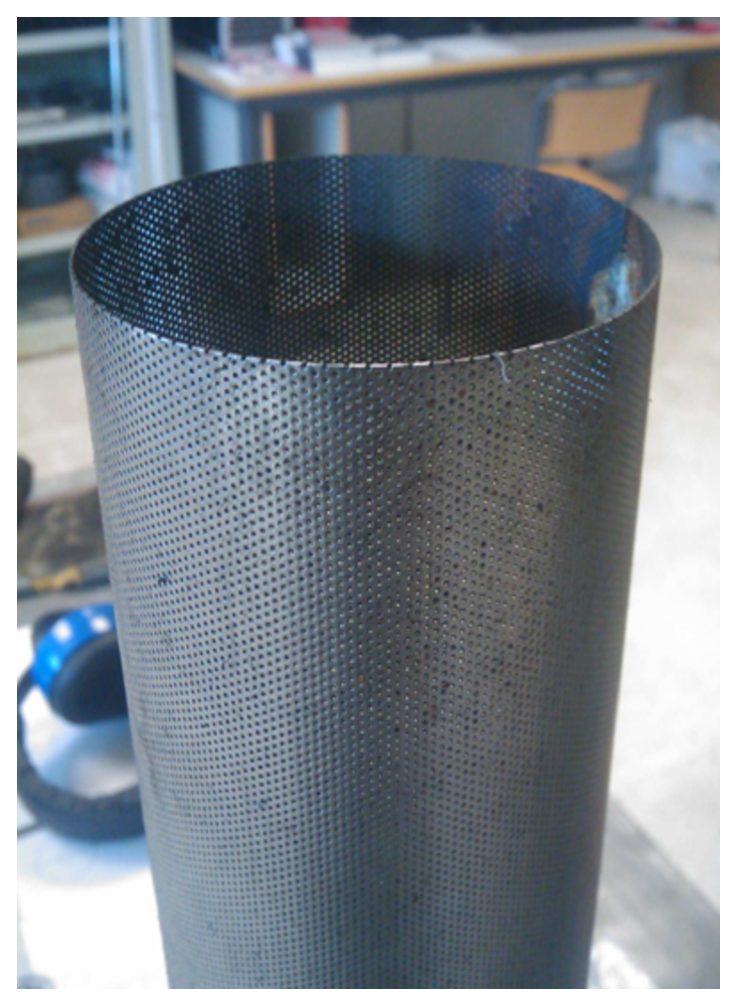
\includegraphics[width = 0.7\linewidth]{singleshell.eps}
\caption{The~perforated metallic cylindrical shell fabricated and used in the~experiments in \cite{garcia1, garcia2, garcia11}.}
\label{fig:singleshellChain}
\end{center}
\end{figure}

Each cylindrical shell is produced by rolling a~perforated metal plate into a~cylindrical shape (see \cref{fig:singleshellChain}).
In this chapter, I will be using the~same material and geometry parameters that were adopted for the~experimental and numerical studies in \cite{garcia1, garcia11}, namely:
\begin{equation*}
\hspace{-5cm}
\begin{array}{lll}
\bullet &\text{outer radius of the~shell} &a=4.00 \text{ cm},\\
\bullet &\text{inner radius of the~shell} &b=3.95 \text{ cm},\\
\bullet &\text{thickness of the~shell } (h=a-b) &h=0.05 \text{ cm},\\
\bullet &\text{radius of the~circular perforation} &r = 0.25 \text{ mm},\\
\bullet &\text{filling fraction of the~perforations} &\sigma = 0.145.\\
\end{array}
\end{equation*}


The~metal from which the~shells were made of was aluminum, and the~parameters of the~air environment are as follows:
\begin{equation*}
\hspace{-6.5cm}
\begin{array}{lll}
\bullet &\text{density of air} &\rho_0=1.25 \text{ kg/m}^3,\\
\bullet &\text{speed of sound in air} &c_0=343 \text{ m/s},\\
\bullet &\text{viscosity of air (dynamic)} &\eta_0 = 17.8\,\mu\text{Pa}\cdot\text{s}.\\
\end{array}
\end{equation*}

The~interaction of the~perforated shell with the~sound, specifically, the~boundary conditions at the~metal-air interfaces, will be described by the~effective impedance $Z_p$ of the~shell.


\section{Impedance of the~Perforated Scatterer}

The~notion of effective impedance was introduced in the~works \cite{maa,maa2} for flat thin perforated plates, and it differs essentially from the~notion of the~acoustic impedance of the~medium $Z=\rho c$.
For a~plate of thickness $h$ coinciding with the~$xOy$ plane, the~effective impedance was defined as
\begin{equation}
\label{eq:impedanceChain}
Z_p~=~\frac{\left.p\right|_{z=-\frac{h}{2}}-\left.p\right|_{z=+\frac{h}{2}}}{\bar{v}_z},
\end{equation}
where the~pressures in the~numerator are evaluated on either side of the~plate, and the~denominator expresses the~$z$-component of the~average velocity of the~fluid inside the~perforation.

This idea of the~effective impedance comes with additional assumptions.
First of all, it relies on the~high contrast between the~material of the~plate and the~environment.
This condition is satisfied when experimenting with metal plates in air, and therefore one may assume the~metal regions to be ideally rigid.
Then, the~transmission of sound through the~perforated plate occurs mostly through the~perforations.
The~plate is assumed to be perforated uniformly with a~quite high perforation constant, so that a~single boundary condition would apply for the~entire plate regardless of where the~openings are actually located.
This boundary condition takes the~form of
\begin{equation}
\label{eq:bcChain}
\left.v_z\right|_{z=-\frac{h}{2}}~=~\left.v_z\right|_{z=+\frac{h}{2}}~=~\frac{\left.p\right|_{z=-\frac{h}{2}}-\left.p\right|_{z=+\frac{h}{2}}}{Z_p},
\end{equation}
where due to the~small thickness of the~plate the~velocities on either side of the~plate are approximately equal.
Also, the~wavelength of sound that penetrates through the~plate must be much larger than the~perforation size.

The~expression for $Z_p$ through the~material parameters and the~perforation geometry is typically represented as a~sum of internal and external terms which capture different physical aspects of the~sound propagation.


\subsection{Internal Contribution of a~Single Perforation}

The~internal term is the~most important for the~total effective impedance since it describes the~propagation of sound through the~perforation.
The~derivation of this term outlined in \cite{maa} is based on the~studies of wave propagation inside infinitely long tubes \cite{rayleigh2}.

The~motion of the~fluid inside the~perforation can be described by the~linearized Navier-Stokes equation
\begin{equation}
-\nabla p + \eta_0 \Delta \mathbf{v}~=~\rho_0\frac{\partial \mathbf{v}}{\partial t}
\end{equation}
which accounts for the~friction losses due to the~dynamic viscosity of the~fluid.
The~equation of motion along $z$ (in the~axial direction) is conveniently expressed in cylindrical coordinates $(r',\varphi,z)$ as
\begin{equation}
-\nabla_z p+\frac{\eta_0}{r'}\frac{\partial}{\partial r'} \left(r' \frac{\partial v_z}{\partial r'}\right)~=~\rho_0 \frac{\partial v_z}{\partial t}.
\end{equation}

For a~monochromatic vibration (with time dependence $e^{-i\omega t}$) inside the~circular tube of radius $r$, the~latter equation becomes
\begin{equation}
\left(\frac{\partial^2}{\partial r'^2}+\frac{1}{r'}\frac{\partial}{\partial r'}+i\frac{s^2}{r^2}\right)v_z~=~\frac{1}{\eta_0}\frac{\partial p}{\partial z},
\end{equation}
where $s=r/\delta=r\sqrt{\omega\rho_0/\eta_0}$ has the~meaning of the~perforate constant of the~metal plate.
The~parameter $s$ relates the~radius of the~perforation to the~characteristic thickness of the~viscous boundary layer $\delta=\sqrt{\eta_0/\omega\rho_0}$.
For the~large values of $s$ ($s \gg 1$) the~viscous dissipation occurs within the~negligibly thin layers near the~metal surface.

The~boundary condition for the~viscous flow requires vanishing of the~axial velocity at the~walls of the~tube, $\left.v_z\right|_{r'=r}=0$, and this results in the~velocity profile
\begin{equation}
v_z~=~\frac{1}{i\omega\rho_0}\frac{\partial p}{\partial z}\left(1-\frac{J_0\left(s\sqrt{i}\,\dfrac{r'}{r}\right)}{J_0\left(s\sqrt{i}\right)}\right).
\end{equation}
Averaging the~velocity over the~cross section of the~tube gives
\begin{equation}
\bar{v}_z~=~\frac{2}{r^2}\int\limits_{0}^{r}v_z r' dr'~=~\frac{1}{i\omega\rho_0}\frac{\partial p}{\partial z} \left(1-\frac{2}{s\sqrt{i}}\frac{J_1\left(s\sqrt{i}\right)}{J_0\left(s\sqrt{i}\right)}\right),
\end{equation}
and since for a~thin perforated plate one can replace the~pressure gradient with the~ratio of the~pressure difference to the~plate thickness, the~internal term of the~effective impedance \cref{eq:impedanceChain} becomes equal
\begin{equation}
Z_1^{(int)}~=~-i\omega\rho_0 h \left(1-\frac{2}{s\sqrt{i}}\frac{J_1\left(s\sqrt{i}\right)}{J_0\left(s\sqrt{i}\right)}\right)^{-1}.
\end{equation}


\subsection{External Contribution of a~Single Perforation}

I write the~external term of the~effective impedance as
\begin{equation}
Z_1^{(ext)}~=~4\sqrt{2\eta_0\omega\rho_0}-i\omega\rho_0\frac{16r}{3\pi}\left(1-2.5\sqrt{\frac{\sigma}{\pi}}\right).
\end{equation}
The~first contribution is a~viscous end correction \cite{guo} which is due to the~dissipation of acoustic energy near (not inside) the~opening.
The~second term appears as a~result of the~air motion outside the~hole.
Qualitatively, the~latter effect is accounted for by increasing the~effective depth of the~perforation and is viewed as an~extra mass attachment to the~edges of the~hole \cite{crandall,ingard}.

Other possible additions to the~impedance may be due to the~nonlinear or the~grazing flow effects, which are disregarded in this chapter.


\subsection{Total Impedance}

Now, the~impedance $Z_1 = Z_1^{(int)}+Z_1^{(ext)}$ of a~single perforation needs to be related to the~impedance of the~whole plate.
In order to do that, I separately consider the~points on both surfaces of the~plate that correspond to either the~hole or the~metal, and write down how the~velocities of the~acoustic vibrations in air at these points are related.

Namely, I conclude that
\begin{equation}
\label{eq:metalvsholeChain}
\left.v_z\right|_{z=\pm\frac{h}{2}}~=~
\left[\begin{aligned}
&\hspace{1cm} 0, &(\text{for metal}), \\
&\frac{\left.p\right|_{z=-\frac{h}{2}}-\left.p\right|_{z=+\frac{h}{2}}}{Z_1}, &(\text{for holes}).
\end{aligned}\right.
\end{equation}
The~first relation is dictated by the~rigid-body approximation, and for the~rest of the~points I make use of the~introduced impedance $Z_1$.

In the~case of large wavelengths of sound, $\lambda \gg r/\sqrt{\sigma}$, it is possible to average \cref{eq:metalvsholeChain} over the~element of the~plate surface which has its linear size much smaller than $\lambda$ but nevertheless contains a~large number of perforations.

The~averaging results in the~uniform boundary condition
\begin{equation}
\label{eq:boundaryconditionChain}
\left.v_z\right|_{z=\pm\frac{h}{2}}~=~\frac{\left.p\right|_{z=-\frac{h}{2}}-\left.p\right|_{z=+\frac{h}{2}}}{Z_p},
\end{equation}
where the~effective impedance of the~perforated plate is expressed as
\begin{equation}
\label{eq:ZpChain}
Z_p~=~\frac{Z_1}{\sigma}~=~-\frac{i\omega\rho_0}{\sigma} \left[ h \left(1-\frac{2}{s\sqrt{i}}\frac{J_1\left(s\sqrt{i}\right)}{J_0\left(s\sqrt{i}\right)}\right)^{-1} + 4i\sqrt{2}\delta + \frac{16r}{3\pi}\left(1-2.5\sqrt{\frac{\sigma}{\pi}}\right) \right].
\end{equation}
In the~limit of an~ideal fluid, for which the~viscosity is negligible, $\eta_0 \rightarrow 0$, the~perforate constant approaches infinity, $s\rightarrow\infty$, and the~impedance \cref{eq:ZpChain} becomes purely imaginary
\begin{equation}
\label{eq:ZpIdealChain}
Z_p = -\dfrac{i\omega\rho_0 }{\sigma} \left[h + \dfrac{16r}{3\pi}\left(1-2.5\sqrt{\dfrac{\sigma}{\pi}}\right)\right].
\end{equation}

The~latter expression for the~effective impedance assumes that the~perforated plate is perfectly flat, however, it may still be approximately valid after the~plate is rolled up to form a~cylindrical shell, at least, in the~long-wavelength limit.
The~evidence for this was reported in \cite{garcia2,deraa2}, where the~scattering of sound from the~perforated shell was measured experimentally and compared with the~numerical simulations that employed the~effective impedance \cref{eq:ZpChain}.
The~obtained spectra of the~scattered sound agreed well in the~frequency range from 0 to 5 kHz.



%%%%%%%%%%%%%%%%%%%%%%%%%%%%%%%%%%%%%%%%%%%%%%%%%%%%%%%%%%%%%%%%%%%%
\section{Scattering Problem}

\subsection{Geometry}

\begin{figure}
\begin{center}
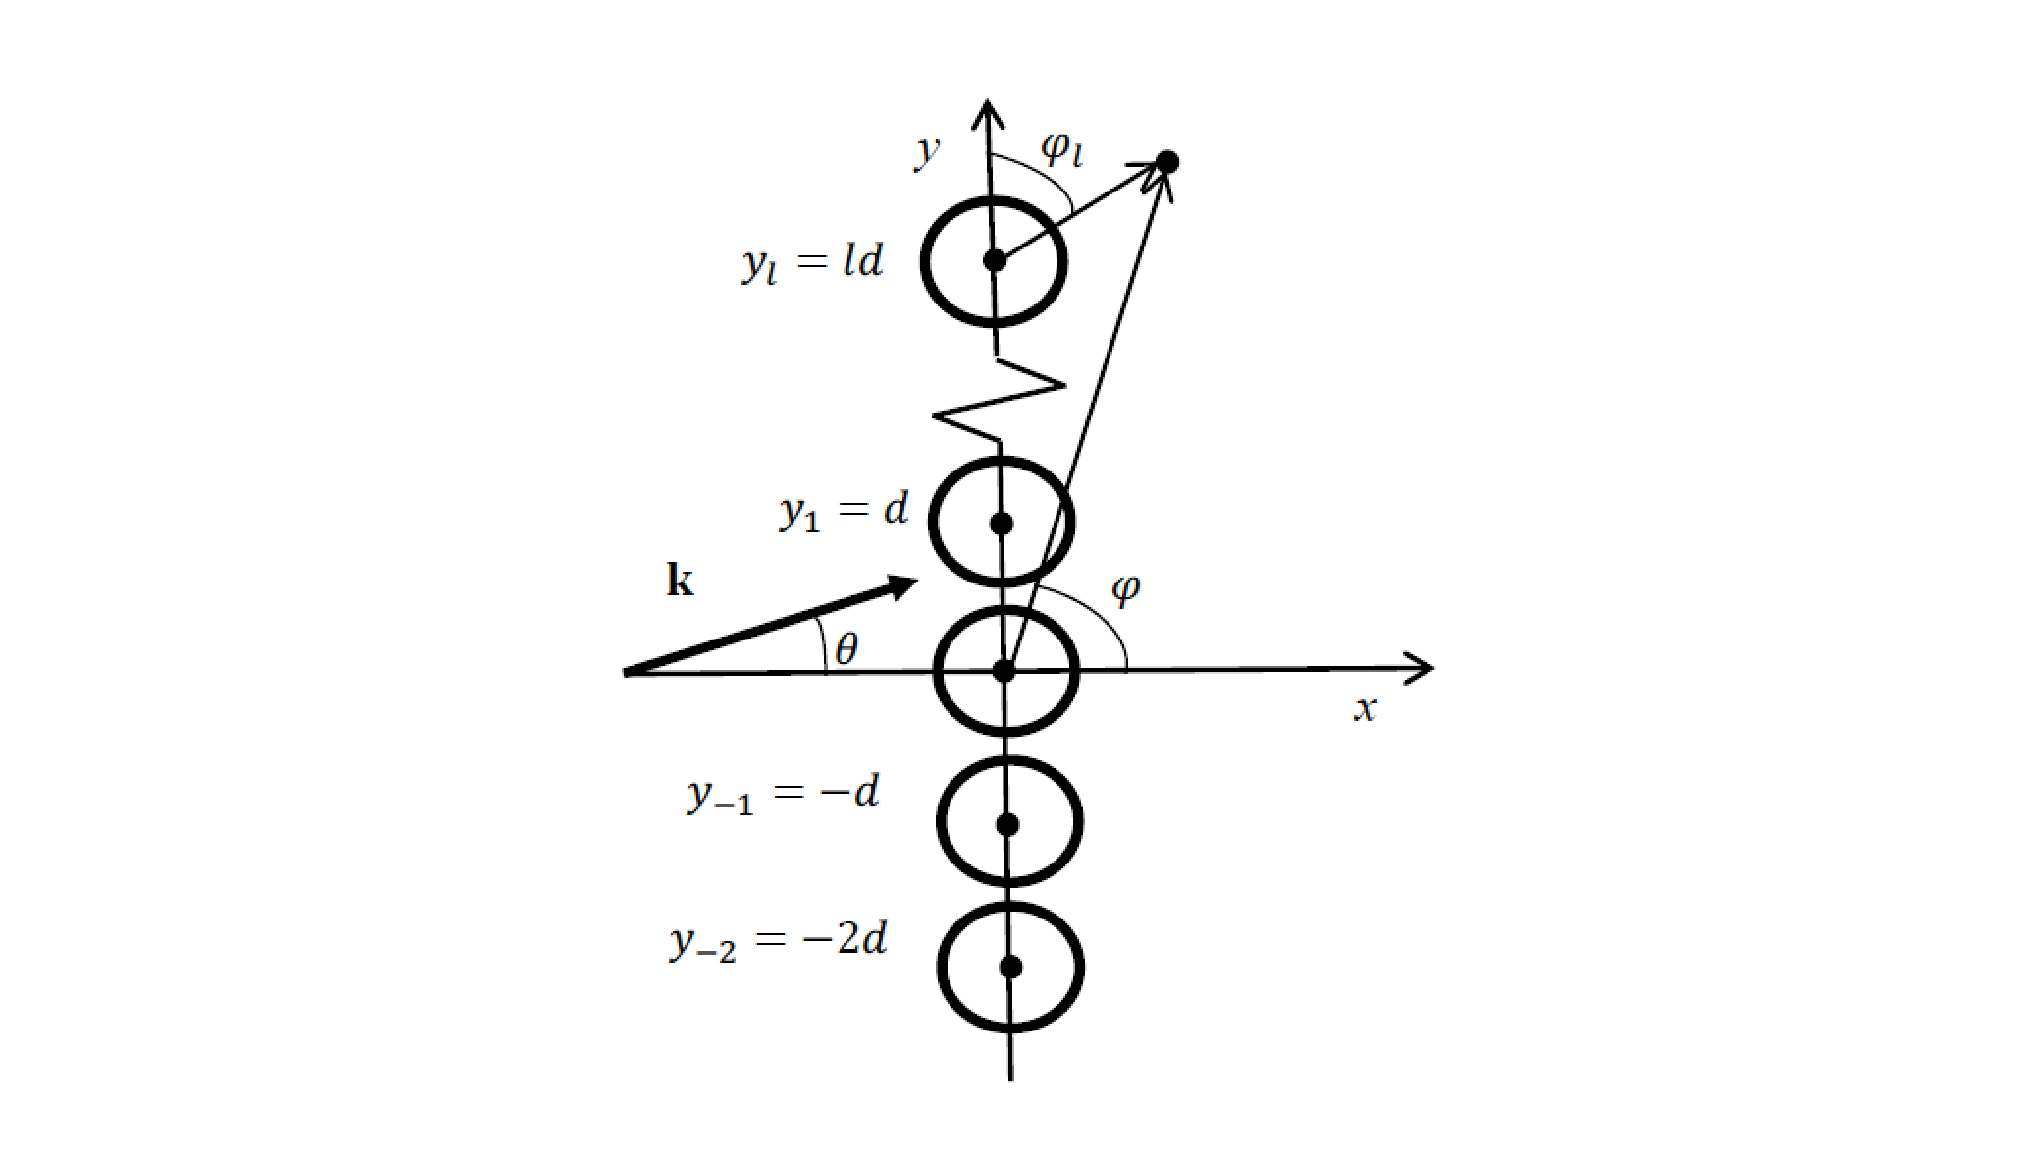
\includegraphics[width=\linewidth]{chaingeometry.eps}
\caption{Top view of the~perforated cylindrical shells aligned along the~$y$-axis with the~period $d$. Polar angles are shown for the~central ($l=0$) and $l$-th units. The~acoustic plane wave is incident at the~angle $\theta$ on the~chain.}
%The~Cartesian coordinates ${\bf r}=(x,y)$ are related to the~polar coordinates $(r_l,\varphi_l)$ associated with the~center of the~$l$-th cylinder: $x=r_l \cos\varphi_l$, $y=y_l + r_l \sin \varphi_l$.}%
\label{fig:geometryChain}
\end{center}
\end{figure}

I start with the~analysis of the~sound interaction with the~finite chain of $2N+1$ scatterers.
The~scatterers are spread along a~straight line, with their axes intersecting the~$y$-axis at the~points $y_n = nd$, $n=0,\pm1,\pm2,\dots, \pm N$ (see \cref{fig:geometryChain}).
The~neighboring shells are separated by a~distance $d=11.0$ cm, which serves as the~period of the~chain.
The~incoming sound is modeled by a~monochromatic plane wave which approaches from the~left at an~angle $\theta$.
Namely, the~pressure of the~incident wave is $p({\bf r},t)=p_0\exp(i{\bf k\cdot r} -i \omega t)$, where the~wave vector ${\bf k}$ has the~components of ${\bf k} = (k_x,k_y,0) = (k \cos\theta,k \sin\theta,0)$.

The~solution to the~scattering problem will be obtained for both finite and infinite chains of perforated shells.
The~latter only requires taking the~limit of $N\rightarrow\infty$, and allows for additional simplifications as the~Bloch theorem becomes applicable.
Similar problems were investigated in \cite{sainidou,zhang}.
The~two dealt with the~scattering of acoustic waves at a~periodic array of solid spheres in fluid and at a~monolayer of elastic spheres in air, respectively.
Also, such scattering problems are of interest in electrodynamics as well, namely, the~work \cite{vergeles} presented an~analysis of the~reflection of electromagnetic waves from an~infinite line of conducting cylinders.

In general, scattering of waves by an~infinite periodic array of cylinders constitutes one of the~classical problems in the~theory of diffraction.

%Scattering of waves by an~{\it infinite} periodic chain of cylinders is one of the~classical problems of theory of diffraction. For conducting cylinders illuminated by an~electromagnetic wave the~expansion of the~scattered field was proposed in \cite{vergeles}. For sound waves, the~field distribution resulting from diffraction in a~periodic array of solid spheres in fluid was calculated in \cite{zhang}. A~similar problem for elastic waves scattered by a~monolayer of elastic spheres was solved in \cite{sainidou}. In these studies, the~chain of scatterers was considered to be infinite, i.e., the~Bloch theorem was applicable. Here we first calculate the~acoustic field scattered by a~finite-length chain. A~periodic infinite chain is analyzed in the~next section.



\subsection{Scattered and Transmitted Pressure Fields}

Based on the~geometry of the~problem, it is convenient to develop the~solution in the~cylindrical coordinate system.
Each cylindrical shell will have a~separate coordinate system associated with it, and I will use the~notion of $(r_l,\varphi_l,z)$ for the~coordinates of a~point in space with respect to the~$l$-th coordinate system.
The~origin of each system is located at the~point $y_l=ld$, i.e., the~axis of each cylinder coincides with the~$z$-axis of the~respective coordinate system, as shown in \cref{fig:geometryChain}.

The~incoming pressure plane wave
\begin{equation}
p({{\bf r},t}) = p_0 \exp(i {\bf k \cdot r}-i \omega t)
\end{equation}
is represented in each of those coordinate systems by the~series
\begin{equation}
\label{eq:3Chain}
p({{\bf r},t})~=~{p}\left(r_l,\varphi_{l},t \right) = p_0 e^{i k r_l\cos\left(\varphi_l-\theta\right)-i \omega t}
~=~p_0\sum\limits_{n=-\infty}^{\infty}i^{n} J_{n}\left(k r_l\right) e^{i n\left(\varphi_l-\theta\right) -i \omega t}.
\end{equation}
where the~wave vector $k$ is $k=\omega/c_0$.
The~harmonic time dependence $e^{-i \omega t}$ will be omitted further below.

The~pressure field obeys the~wave equation \cref{eq:waveeqPRayleigh}, which in the~cylindrical coordinates is expressed as
\begin{equation}
\label{eq:waveeqPCylChain}
\frac{1}{r}\frac{\partial}{\partial r}\left(r\frac{\partial p}{\partial r}\right) + \frac{1}{r^2}\frac{\partial p}{\partial \varphi^2} + k^2 p(r,\varphi)~=~0.
\end{equation}
The~derivative with respect to $z$ does not appear above as the~problem is assumed to be uniform along $z$.
If the~angular dependence is eliminated by assuming the~proportional to $e^{in\varphi}$, $n=0,\pm1,\pm2,...$, behavior of pressure, then the~solutions of the~radial part of the~wave equation \cref{eq:waveeqPCylChain} are the~Bessel functions of the~order $n$.

This knowledge allows to write down the~acoustic field scattered by an~array of shells as a~superposition of cylindrical waves:
\begin{equation}
\label{eq:4Chain}
p_{sc}(r,\varphi) = \sum\limits_{l'} \sum\limits_{n=-\infty}^{+\infty} B_{l'n} H_{n}^{(1)}\left(k r_{l'}\right) e^{i n \varphi_{l'}}, \qquad r_l' \geq a.
\end{equation}
The~inner sum over $n$ represents the~total field radiated by each $l'$-th shell with respect to the~coordinate system aligned with that shell.
The~outer sum over $l'$ adds those contributions together to produce the~total scattered field.
The~value of $l'$ runs from $-N$ to $N$ for a~finite chain, or from $-\infty$ to $+\infty$ for an~infinite chain.
The~Hankel functions of the~first kind $H_n^{(1)}(kr)$ (or simply $H_n(kr)$) are chosen for the~expansion \cref{eq:4Chain} as they describe the~outgoing waves due to their asymptotic behavior $H_n^{(1)}(kr) \sim e^{ikr}/\sqrt{kr}$ at infinity.

The~use of multiple coordinate systems within the~same equation \cref{eq:4Chain} is perplexing and undesirable, and it is best to rewrite the~expression of the~scattered pressure field in terms of only the~coordinates $(r_l, \varphi_l)$ of the~certain $l$-th system.
Fortunately, since one has a~trivial relation between the~Cartesian coordinates ${\bf r}=(x,y)$ and the~polar coordinates $(r_l,\varphi_l)$ in the~form of 
\begin{align}
x~&=~r_l \cos\varphi_l, \\
y~&=~ld + r_l \sin \varphi_l,
\end{align}
then the~transformation between $(r_l,\varphi_l)$ and $(r_{l'},\varphi_{l'})$ is as follows:
\begin{align}
r_{l'} \cos\varphi_{l'}~&=~r_l \cos\varphi_l, \label{eq:5aChain} \\
r_{l'} \sin\varphi_{l'}~&=~(l-l')d + r_l \sin \varphi_l, \label{eq:5bChain}
\end{align}
For the~polar coordinates related by \cref{eq:5aChain}-\cref{eq:5bChain}, the~Graf's addition theorem (see Appendix \ref{appGrafTheorem}) applies:
\begin{equation}
\label{eq:6Chain}
H_{n}(k r_{l'}) e^{in \varphi_{l'}} = \sum\limits_{n'=-\infty}^{\infty}i^{(n+n') \sign(l-l')} H_{n+n'}(k |l-l'| d) J_{n'}(k r_l) e^{i n'(\pi- \varphi_l)},
\end{equation}
given that the~conditions $l' \neq l$ and $r_l<|l-l'|d$ are met.

As a~result, one arrives at the~expression for the~scattered field \cref{eq:4Chain} that involves only one pair of coordinates $(r_l, \varphi_l)$ and is valid for $r_l<d$, i.e., only in the~vicinity of the~$l$-th perforated shell:
\begin{align}
\label{eq:7Chain}
p_{sc}(r_l,\varphi_l) = \sum\limits_{n=-\infty}^{+\infty} \Bigg[&B_{ln} H_{n}\left(k r_l\right) e^{i n \varphi_l}+ \Bigg.\\
+\Bigg. &\sum\limits_{l' \neq l} B_{l'n}\sum\limits_{n'=-\infty}^{+\infty}i^{(n+n')\sign(l-l')}H_{n+n'}\left(k |l-l'| d\right) J_{n'}\left(k r_l\right) e^{i n'(\pi - \varphi_l)} \Bigg]. \notag
\end{align}
The~obtained expansion will prove extremely useful for the~purpose of dealing with the~boundary conditions at the~surfaces of the~shells.

As for the~pressure fields inside each $l$-th cylinder, I write their expansions over the~Bessel functions
\begin{equation}
\label{eq:8Chain}
p_{in}^{(l)}(r_l,\varphi_l) = \sum_{n=-\infty}^{\infty} {C_{ln} J_n(k r_l)e^{in \varphi_l}}, \qquad r_l \le b.
\end{equation}
All other cylinder functions are still valid solutions of the~wave equation \cref{eq:waveeqPCylChain}, but they cannot enter the~series \cref{eq:8Chain} as they diverge when $r_l\rightarrow 0$ and therefore do not describe any physically reasonable field behavior.



\subsection{Boundary Conditions at the~Surfaces of the~Shells}

As was discussed earlier, the~acoustic fields on either side of the~perforations are related in a~simplified fashion which, nevertheless, does not undermine the~resulting accuracy of calculations.
Namely, even though each perforated shell has a~finite thickness $h$, its value is much smaller than either of the~radii $a$ and $b$, and thus one can view the~two cylindrical faces of each shell as a~virtually single interface.
The~fluid-metal interactions are already encompassed inside the~effective impedance \cref{eq:ZpChain}, and one only needs to relate the~pressure fields outside the~shells with those inside the~shells.
 
The~condition \cref{eq:bcChain} prescribes to assume the~radial component of the~velocity of the~fluid (that is, normal to the~interface) to be unchanged across the~thickness of the~metal, and also relates it to the~pressure discontinuity between the~faces of the shells:
\begin{equation}
\label{eq:9Chain}
v_r|_{r=a} = v_r|_{r=b} = \dfrac{p|_{r=b} - p|_{r=a}}{Z_p}
\end{equation}

The~radial velocity in fluid is derived from the~local pressure according to \cref{eq:vandpRayleigh}:
\begin{equation}
\label{eq:10Chain}
v_r = \dfrac{1}{i\omega\rho_0}\dfrac{\partial p}{\partial r}.
\end{equation}

From the~three equations that appear in \cref{eq:9Chain}, I will be using the~following two independent relations:
\begin{align}
\label{eq:10aChain}
v_r|_{r=a}~&=~v_r|_{r=b}, \\
p|_{r=a}~&=~p|_{r=b}-Z_p v_r|_{r=b},
\end{align}
where the~place of the~pressure outside the~shell $p|_{r=a}$ will be taken by the~superposition of the~incoming and scattered waves $p+p_{sc}$, and the~pressure inside the~shell $p|_{r=b}$ is exactly the~pressure field $p_{in}^{(l)}$.

The~method of expressing the~acoustic fields in terms of series over cylinder functions and matching them via the~boundary conditions is exact since its solution is the~total \textit{true} field.
As opposed to this, the~approach based on the~$T$-matrix method and the~multiple scattering theory used in \cite{garcia2,garcia1} is only approximate as it discards the~high-order scatterings of the~waves.

The~dissipation of energy due to the~viscous effects in air is accounted for via the~effective impedance $Z_p$ of the~perforated shells.
The~viscous friction at the~air-metal interfaces is practically the~only reason for the~energy loss.
The~dissipation within the~bulk volume of air is almost nonexistent at the~frequencies of several kHz, the~typical decay length being on the~order of several kilometers.

Note that since the~elastic vibrations of the~metal are not considered explicitly in this approach, there is neither need nor advantage in using the~notion of acoustic potentials \cref{eq:waveeqBRayleigh,eq:waveeqLRayleigh,eq:waveeqSRayleigh} in solving this problem.


\section{Solution for the~Scattered Acoustic Field}

\subsection{Finite Chain of Perforated Shells}

The~equations \cref{eq:3Chain}, \cref{eq:7Chain}, and \cref{eq:8Chain} express the~pressure fields basically in the~form of Fourier expansions over $e^{in\varphi_l}$.
Because of that, the~angular dependence in the~boundary conditions \cref{eq:10Chain} can be eliminated by applying the~Fourier transform,
splitting each condition into a~set of equations for the~respective Fourier coefficients.
This results in the~following set of linear equations for the~unknowns $B_{ln}$ and $C_{ln}$:

\begin{equation}
\label{eq:11Chain}
\left\{
\begin{array}{rll}
C_{ln} \dfrac{J'_{n}\left(k b\right)}{J'_{n}\left(k a\right)}~&=~p_0 i^n e^{-i n\theta} &+ B_{ln} \dfrac{H'_{n}\left(k a\right)}{J'_{n}\left(k a\right)} + \\
& &+ \dsum\limits_{l' \neq l} \dsum\limits_{n'=-\infty}^{\infty} i^{(n-n')\sign(l-l')}H_{n-n'}(k|l-l'|)d) B_{l'n'},\\
 & & \\
%
%
\dfrac{i k Z_p}{\omega\rho_0}\,C_{ln} \dfrac{J'_{n}\left(k b\right)}{J_{n}\left(k a\right)} + C_{ln} \dfrac{J_{n}\left(k b\right)}{J_{n}\left(k a\right)}~&=~p_0 i^n e^{-i n\theta} &+ B_{ln} \dfrac{H_{n}\left(k a\right)}{J_n\left(k a\right)} + \\
& &+ \dsum\limits_{l' \neq l} \dsum\limits_{n'=-\infty}^{\infty} i^{(n-n')\sign(l-l')}H_{n-n'}(k|l-l'|)d) B_{l'n'}.\\
\end{array}
\right.
\end{equation}
The~index $n$ indicates which specific Fourier component the~equations are written for, and the~index $l$ enumerates the~shells, meaning that the~equations containing $C_{ln}$ resulted from applying the~boundary conditions to the~$l$-th shell.

The~scattered acoustic field depends only on the~unknown $B_{ln}$, so one may substitute the~value of $C_{ln}$ obtained from the~first row of \cref{eq:11Chain} into the~second row, and obtain the~system of linear inhomogeneous equations for $B_{ln}$ only:
\begin{equation}
\label{eq:12Chain}
\mathcal{S}_n B_{ln} + \sum\limits_{l' \neq l} \sum\limits_{n'=-\infty}^{\infty} i^{(n-n')\sign(l-l')} H_{n-n'}\Big(k|l-l'|d\Big) B_{l'n'} = -p_0 i^n e^{-i n\theta},
\end{equation}
where $\mathcal{S}_n$ denotes the~fraction
\begin{equation}
\label{eq:13Chain}
\mathcal{S}_n = \dfrac{H_n\left(k a\right)-H'_n\left(k a\right)\left(\dfrac{i Z_p}{\rho_0 c_0}+\dfrac{J_{n}\left(k b\right)}{J'_{n}\left(k b\right)}\right)}{J_n\left(k a\right)-J'_n\left(k a\right)\left(\dfrac{i Z_p}{\rho_0 c_0}+\dfrac{J_{n}\left(k b\right)}{J'_{n}\left(k b\right)}\right)}.
\end{equation}
The~last step in calculating the~distribution of the~scattered field \cref{eq:4Chain} from a~finite chain of perforated shells is solving the~linear set \cref{eq:12Chain}, which will be done numerically.


\subsection{Infinite Chain of Perforated Shells}

For an~infinite periodic chain of scatterers ($N=\infty$), the~obtained system \cref{eq:12Chain} still remains valid.
Moreover, it can be now further simplified since it is imperative to benefit from the~established periodicity of the~system along the~$y$-axis.
The~Bloch theorem guarantees that in a~periodic environment a~propagating wave $\psi(x,y)$ is represented as $\psi(x,y)~=~e^{iqy}\upsilon(x,y)$, where the~function $\upsilon(x,y)$ is periodic, $\upsilon(x,y)=\upsilon(x,y+d)$, and $q$ is the~$y$-component of the~ wavevector of the~wave.

The~incident at the~chain plane wave determines the~wavevector $q$:
\begin{equation}
q~=~k_y~=~k\sin\theta,
\end{equation}
and to satisfy the~inferences of the~Bloch theorem, the~unknown amplitudes $B_{ln}$ must be related to the~values $B_{0n}$ associated with the~shell in the~middle of the~chain:
\begin{equation}
\label{eq:14Chain}
B_{ln} = e^{ik_yld} B_{0n}.
\end{equation}
I substitute the~latter relation into \cref{eq:12Chain}, redefine the~unknowns as $b_n=i^{-n}B_{0n}$, and arrive at the~following set of linear equations:
\begin{equation}
\label{eq:15Chain}
\mathcal{S}_n b_{n} + \sum\limits_{n'=-\infty}^{\infty} F(n'-n) b_n' = -p_0 e^{-i n\theta}, \,\, n=0,\pm1,\pm2,\dots
\end{equation}
Here the~lattice sum $F(n)$ is an~infinite series
\begin{equation}
\label{eq:latticesum}
F(n)= \sum\limits_{l'=1}^{+\infty} H_{n}\left(k l'd\right) \left[e^{i k_y l' d} + (-1)^{n} e^{-i k_y l' d}\right],
\end{equation}
the~calculation of which is discussed in Appendix \ref{appConvSeries}.

A~similar set of equations was obtained in \cite{vergeles,evans} for scattering of waves at an~infinite periodic chain of metallic cylinders.




\section{Eigenmodes of an~Infinite Chain of Scatterers}


\subsection{Dispersion Relation}

\begin{figure}
\begin{center}
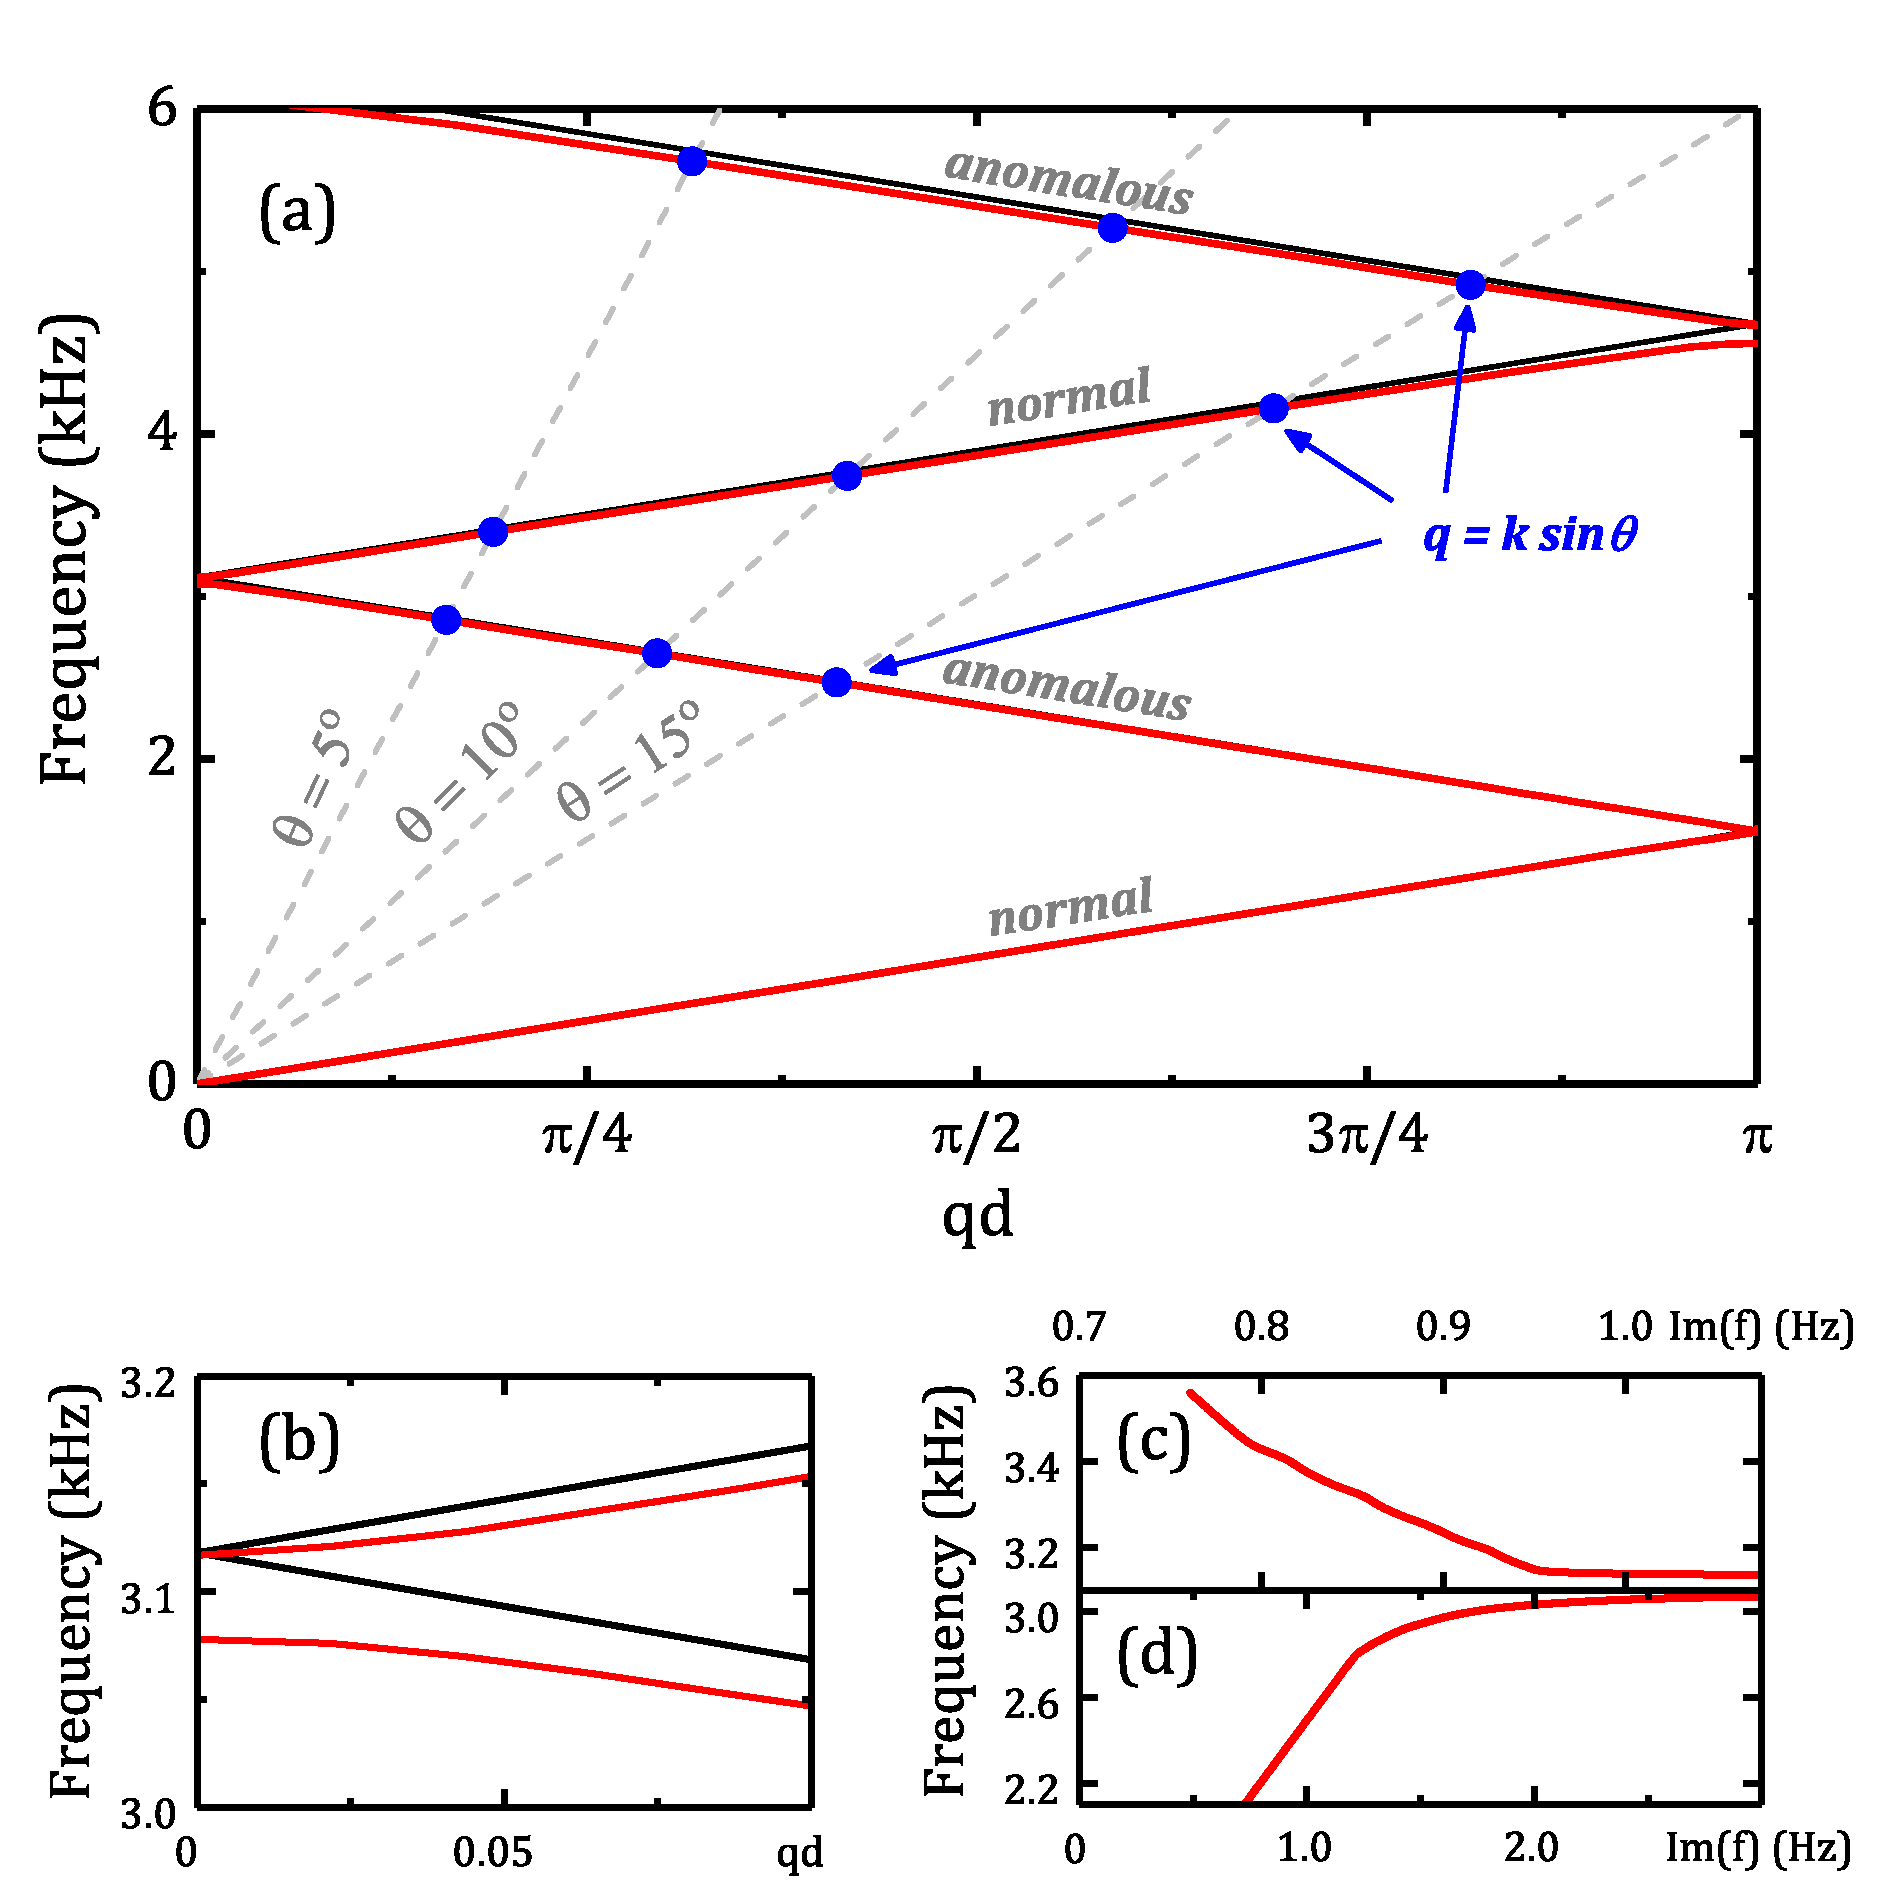
\includegraphics [width=0.9\linewidth]{dispChain.eps}
\caption{(a) Band structure of an~infinite periodic chain of shells in inviscid air environment. Straight black lines show linear dispersion in air. Red lines are the~real parts of eigenfrequencies calculated from \cref{eq:17Chain}. Crossings of the~dispersion curves with three dashed straight lines \cref{eq:18Chain} give the~frequencies of resonant coupling of the~incident plane wave to the~eigenmodes of the~chain for three angles of incidence, $\theta = 5^{\circ}$, $\theta = 10^{\circ}$, and $\theta = 15^{\circ}$. (b) Band splitting at the~$\Gamma$-point near the~frequency $f=3.1$ kHz; the~distance between the~levels in the~doublet is 35 Hz. (c),(d) Absolute value of the~imaginary part of eigenfrequency vs its real part for the~region near 3.1 kHz.}
\label{fig:dispChain}
\end{center}
\end{figure}
%\textcolor{red}{The~Wood's anomalies are observed at these resonant frequencies.}  The~horizontal axes, where the~imaginary part of the~frequency is plot, are different for the~upper and lower levels of the~doublet. 

Here I analyze the~eigenmodes that can be supported by the~infinite chain of perforated shells in order to gain additional insights about its capability to suppress sound transmission.
The~eigenmodes are the~waves propagating in either direction along the~chain and are characterized by the~wavevector $q$.
They are the~nontrivial solutions of \cref{eq:15Chain}, in which the~right-hand side contains no incident wave.
By equating the~determinant of a~corresponding homogeneous linear system to zero,
\begin{equation}
\label{eq:17Chain}
\det |\mathcal{S}_n \delta_{nn'} + F(n'-n)|=0,
\end{equation}
one obtains the~equation that defines the~dispersion relation $\omega=\omega(q)$ of the~eigenmodes.

Finding the~solution to \cref{eq:17Chain} is complicated by the~necessity to calculate the~determinant of an~infinite matrix and by having to deal with the~slow-converging series \cref{eq:latticesum}.
The~latter issue is addressed by identically replacing $F(n)$ with the~fast-converging series originally found in \cite{twersky} and subsequently used in \cite{vergeles, evans} (see Appendix \ref{appConvSeries}).

\cref{fig:dispChain}(a) visualizes the~few lowest bands of the~dispersion equation, which are calculated numerically.
Due to perforated shells being weak scatterers, the~resulting dispersion curve (shown in red) is almost identical to the~band structure describing the~empty-lattice model (shown in black).
The~differences between the~two appear only near the~$\Gamma$-point $q=0$ (and also at the~zone edge $q=\pi/d$), where the~level doublet is formed due to the~level repulsion, forming a~gap.
The~gap size is approximately $35$ Hz between the~second and the~third bands (which is near the~frequency of $3.1$ kHz).
The~first (lowest) band and other odd-numbered bands have normal dispersion, whereas every even-numbered band exhibits anomalous dispersion.
As can be seen in \cref{fig:dispChain}(b), the~dispersion of the~bands becomes essentially nonlinear towards the~$\Gamma$-point.

It is also peculiar that the~two bands of the~doublet exhibit different behavior: only for the~lower band does the~group velocity vanish when $q=0$, thus making the~gap opening strongly asymmetric.
Moreover, the~upper band exhibits a~singularity which is not resolved in \cref{fig:dispChain}.
The~behavior of both bands will be analyzed in more detail further in this chapter.

The~solutions $\omega(q)=2 \pi f(q)$ of the~transcendental dispersion equation \cref{eq:15Chain}, found for real values of the~wave vector $q$, are complex.
This makes the~acoustic eigenmodes of an~infinite chain leaky, regardless of whether the~viscosity of the~fluid is accounted for.
Leaky eigenmodes are not strongly localized in the~vicinity of the~chain, instead they carry the~acoustic energy away from it, and the~imaginary part of the~frequency describes the~strength of radiative decay.

Nevertheless, the~leaky modes may still be long-living excitations if the~decay is very slow, i.e., if the~imaginary part $\im f$ is small.
As is shown in \cref{fig:dispChain}(c,d), the~rate of radiative decay $|\im f|$ is smaller than the~frequency of sound $f \approx \re f$ by at least two orders of magnitude.
Namely, near the~$\Gamma$-point this rate is about $1$-$3$ Hz, which practically does not affect the~width of the~resonance minima in the~transmission spectra, as will be discussed below.
The~use of the~absolute value to characterize the~decay rate $|\im f|$ indicates that the~imaginary part of frequency is negative, $\im f < 0$, which is imperative in order to have the~time-dependent term $e^{-i\omega t}$ exponentially decreasing and not increasing with time.

%The~numerical solution of this dispersion equation for the~few lowest bands is presented in \cref{fig:dispChain}. Since perforated shells are weak scatterers, the~dispersion curve (blue dots) is very close to the~band structure obtained in the~empty-lattice model, shown by the~straight broken line (red). Only at the~$\Gamma$-point $q=0$ (and at the~edge $q=\pi/d$) the~effect of level repulsion leads to gap opening of 35 Hz and essentially nonlinear dispersion, see the~left insert to \cref{fig:dispChain}. It is shown in Appendix B \textcolor{red}{!!!} that near the~point of degeneracy, $f = 3078$ Hz, the~upper and lower bands exhibit different behavior. In particular, the~gap opening is strongly asymmetric and the~group velocity vanishes at $q=0$ only for the~lower band. There are also some singularities in the~dispersion of the~upper band which are not resolved in \cref{fig:dispChain}. They are shown in the~insert to \cref{fig:asymgapChain}.  Away from the~$\Gamma$-point the~dispersion of the~both bands is practically linear but it is normal for the~upper band and anomalous for the~lower one.

%For real values of the~wavevector $q$ all the~solutions $\omega(q)=2 \pi f(q)$ of the~transcendental equation \cref{eq:15Chain} are complex. This means that the~acoustic eigenmodes of an~infinite chain of shells are leaky modes, even if the~viscosity of the~fluid is neglected. The~imaginary part of frequency describes weak radiative decay, i.e., the~acoustic eigenmodes are not strongly localized near the~chain.

%However, since the~decay is very slow the~leaky eigenmodes are long-living excitations. The~imaginary part is negative, $\text{Im }f<0$, in order for the~time-dependent factor $e^{-i\omega t}$ to decay with time. The~rate of radiative decay $|\text{Im }f|$ is at least two orders of magnitude smaller than the~frequency of sound $f \approx \text{Re }f$ as it can be seen from the~right insert to \cref{fig:dispChain}. For the~frequencies near the~$\Gamma$-point the~rate of radiative decay is about 1-3 Hz, i.e., it practically does not contribute to the~width of the~resonance minima as will be shown below.



\subsection{Analysis of the~Asymmetric Band Gap}

Here I will analyze the~behavior of the~two bands forming a~doublet near the~$\Gamma$-point (see \cref{fig:dispChain}(c)).
This can be done using an~approach that treats the~perforated shells as a~small perturbation to the~uniform air background.
In zero approximation, i.e., in the~empty-lattice model, the~dispersion bands are linear.
When the~small perturbations are introduced, the~differences between the~linear bands and the~actual dispersion curves found by solving \cref{eq:17Chain} are small, and are only significant in the~vicinity of the~$\Gamma$-point and the~edges of the~Brillouin zone, i.e., only near the~points of degeneracy.
In the~theory of band structures, the~perturbation theory for degenerate states is typically used to calculate such band corrections.
However, the~degeneracy is removed from the~picture by the~presence of weak scattering, and the~narrow band gaps are formed.
In solids, applying such perturbation theory results in the~so-called nearly free electron model, where the~unperturbed eigenfunctions are represented by a~basis of simple plane waves.
In the~case of a~chain of perforated shells, the~basis of cylindrical functions needs to be used, and thus the~perturbation theory that will apply here will strongly differ from that in the~nearly free electron model.
Even though the~final result --- forming of narrow band gaps --- is expected to be qualitatively the~same, I will still obtain the~explicit expressions for the~level repulsion near the~points of degeneracy and compare obtained formulas with the~values found by solving the~exact dispersion equation \cref{eq:17Chain} numerically.
I will show that the~strength of the~level repulsion is essentially different from what is known in the~nearly free electron model.
The~reason behind this is the~specific form of the~boundary condition \cref{eq:9Chain}, which approximates the~interaction of the~shell with the~background using the~impedance approach and assumes a~discontinuity of pressure on the~two surfaces of the~shell even for very thin shells.

%Assuming that the~perforated shells are weak scatterers, the~solution of the~dispersion equation \cref{eq:17Chain} can be found using a~perturbation theory. In zero approximation, the~dispersion that corresponds to the~empty-lattice model is linear. Corrections to this linear dispersion are of interest only near the~points of degeneracy, i.e., in the~vicinity of the~$\Gamma$-point and the~edges of the~Brillouin zone.
%In the~theory of band structures, these corrections are usually obtained using perturbation theory for degenerate states. Due to weak scattering, the~degeneracy is lifted, giving rise to narrow band gaps. In solids, this kind of perturbation theory is known as the~nearly free electron model and it uses the~basis of plane waves as unperturbed eigenfunctions. Here we look for the~solution of the~wave equation in the~basis of cylindrical functions that leads to strong modification of the~perturbation theory as compared to the~well-known nearly free electron model.
%While the~final result is the~same -- opening of narrow band gaps, it is worthwhile to get the~explicit formulas for the~gap width and for the~level repulsion near the~points of degeneracy and to compare these formulas with the~results obtained nonperturbatively from the~exact dispersion equation \cref{eq:17Chain}. It will be shown that because of the~specific form of the~boundary condition \cref{eq:9Chain}, which assumes a~discontinuity of pressure even for very thin shell, the~strength of the~level repulsion is quite different from that observed in the~nearly free electron model.

%The~numerical solution of the~dispersion equation \cref{eq:17Chain} showed that the~dispersion of the~chain eigenmodes is linear everywhere except , where the~level repulsion leads to parabolic dispersion.
%\begin{equation}
%\label{B1}
%\det |\mathcal{S}_n \delta_{nn'} + F(n'-n)|=0
%\end{equation}
%Moreover, this solution must become identical to the~empty-lattice model dispersion when there are no shells, which corresponds to the~limit of %vanishing thickness of the~shells, $h = (a - b) \rightarrow 0$, and vanishing impedance, $Z_p \rightarrow 0$.
%Here we develop a~perturbation theory for the~band structure calculation which is formally equivalent to the~nearly free electron model in solids. to find the~analytical solution of the~dispersion equation \cref{eq:17Chain}, where the

The~absence of the~perforated shells, which implies no scattering of sound, can be obtained by decreasing the~acoustic impedance to zero, $Z_p\rightarrow 0$.
This fact makes it different from the~situation where the~absence of scattering from a~solid cylinder is normally realized by matching the~impedances $\rho c$ of the~background fluid and the~cylinder.
The~parameter $Z_p$ will serve as a~small perturbation in the~perturbation theory.
The~smallness of $Z_p$ also requires the~shells to be extremely thin, $h=\left(a-b\right) \rightarrow 0$, however, the~thickness cannot be used as a~small parameter as the~latter condition only is not sufficient itself (see \cref{eq:ZpChain} and \cref{eq:ZpIdealChain}).


%The~scattering of sound by perforated cylinders vanishes when the~acoustic impedance $Z_p\rightarrow 0$. This situation is different from the~case of solid cylinders when absence of scattering requires matching of the~impedance of the~material of the~cylinders and the~impedance $c_0\rho_0$ of the~background fluid.  Thus, the~small parameter of the~perturbation theory is impedance $Z_p$ that requires that the~thickness of the~shell $h=\left(a-b\right) \rightarrow 0$. The~latter condition is necessary but not sufficient, as it is seen from Eqs. \cref{1} and \cref{2}.

The~coefficient $\mathcal{S}_n$ in \cref{eq:13Chain} approaches infinity when $a\rightarrow b$ and $Z_p \rightarrow 0$, which allows rewriting the~dispersion relation \cref{eq:17Chain} in the~following form:
\begin{equation}
\label{eq:B3Chain}
\det \left|\delta_{nn'} + \dfrac{F(n'-n)}{\mathcal{S}_n}\right|=0.
\end{equation}
Since $F(n'-n)/\mathcal{S}_n \ll 1$, the~matrix in \cref{eq:B3Chain} is almost diagonal and its determinant can be approximated by
\begin{equation}
\label{eq:B4Chain}
\det \left|\delta_{nn'} + \dfrac{F(n'-n)}{\mathcal{S}_n}\right| \approx \det |\delta_{nn'}| + \Tr\left( \dfrac{F(n'-n)}{\mathcal{S}_n}\right)
= 1 + F(0)\sum_{n=-\infty}^{+\infty}\mathcal{S}_n^{-1}.
\end{equation}
I further expand the~terms $\mathcal{S}_n^{-1}$ in the~series \cref{eq:B4Chain} over the~small parameters $h=a-b$ and $Z_p$.
In the~linear approximation one arrives at the~expression
\begin{align}
\label{eq:B5Chain}
\mathcal{S}_n^{-1} &= \dfrac{J_n\left(k a\right)-J'_n\left(k a\right)\left(\dfrac{i Z_p}{\rho_0 c_0}+\dfrac{J_{n}\left(k b\right)}{J'_{n}\left(k b\right)}\right)}{H_n\left(k a\right)-H'_n\left(k a\right)\left(\dfrac{i Z_p}{\rho_0 c_0}+\dfrac{J_{n}\left(k b\right)}{J'_{n}\left(k b\right)}\right)} = \\
%
&= \dfrac{-\dfrac{i Z_p}{\rho_0 c_0} J'_{n}\left(k a\right)J'_{n}\left(k b\right) + \Big(J_n\left(k a\right)J'_{n}\left(k b\right)-J'_n\left(k a\right)J_{n}\left(k b\right)\Big)}{-\dfrac{i Z_p}{\rho_0 c_0} J'_{n}\left(k a\right)J'_{n}\left(k b\right) + \Big(H_n\left(k a\right)J'_{n}\left(k b\right)-H'_n\left(k a\right)J_{n}\left(k b\right)\Big)} \approx \notag\\
%
&\approx \dfrac{-\dfrac{i Z_p}{\rho_0 c_0} J'^{2}_{n}\left(k a\right) + k(b-a)\Big(J_n\left(k a\right)J''_{n}\left(k a\right)-J'_n\left(k a\right)J'_{n}\left(k a\right)\Big)}{H_n\left(k a\right)J'_{n}\left(k a\right)-H'_n\left(k a\right)J_{n}\left(k a\right)} = \notag \\
%
&= \dfrac{-\dfrac{i Z_p}{\rho_0 c_0} J'^{2}_{n}\left(k a\right) + k(a-b)\Big(J'^2_n\left(k a\right)-J_n\left(k a\right)J''_{n}\left(k a\right)\Big)}{-\dfrac{2i}{\pi k a}} \approx \notag \\
%
&\approx \dfrac{\pi k a}{2i}\dfrac{i Z_p}{\rho_0 c_0} J'^{2}_{n}\left(k a\right) - \dfrac{1}{2i} \pi k^2 a(a-b) \Big(J'^2_n\left(k a\right)-J_n\left(k a\right)J''_{n}\left(k a\right)\Big). \notag
\end{align}
As is seen from \cref{eq:B5Chain}, the~expansion goes over two dimensionless parameters, $z~=~\dfrac{\pi k a}{2}\dfrac{i Z_p}{\rho_0 c_0}$ and
$\epsilon = \pi k^2 a h$.
Here $k=\omega/c_0$, so these parameters are real if the~background fluid is inviscid.
Since the~impedance $Z_p \propto \omega$ (see \cref{eq:ZpChain}), it follows that $z,\epsilon \propto \omega^2$ as well.
Such quadratic growth invalidates the~approximation \cref{eq:B5Chain} at high frequencies.

After the~expansion \cref{eq:B5Chain} is substituted into the~sum over $n$ in \cref{eq:B4Chain}, one obtains the~following result:
\begin{align}
\label{eq:B6Chain}
\sum_{n=-\infty}^{+\infty}\mathcal{S}_n^{-1} &= \dfrac{\pi k a}{2i}\dfrac{i Z_p}{\rho_0 c_0} \sum_{n=-\infty}^{+\infty} J'^{2}_{n}\left(k a\right) - \dfrac{1}{2i} \pi k^2 a h \sum_{n=-\infty}^{+\infty} \Big(J'^2_n\left(k a\right)-J_n\left(k a\right)J''_{n}\left(k a\right)\Big) = \notag \\
&= \dfrac{\pi k a}{4i}\dfrac{i Z_p}{\rho_0 c_0} - \dfrac{1}{2i} \pi k^2 a h = \frac{z - \epsilon}{2i}.
\end{align}
The~identities $\dsum_{n=-\infty}^{+\infty} J'^2_n(x) = -\dsum_{n=-\infty}^{+\infty} J_n(x) J''_n(x)=\frac12$ were employed here to simplify the~latter expression.
I finally rewrite \cref{eq:B3Chain} and \cref{eq:B4Chain} as
\begin{equation}
\label{eq:BB7Chain}
\frac{1}{F(0)} = -\sum_{n=-\infty}^{+\infty}\mathcal{S}_n^{-1} = -\frac{z - \epsilon}{2i}.
%= i\left(-\dfrac{\pi k a}{4}\dfrac{i Z_p}{\rho_0 c_0} + \dfrac12 \pi k^2 a (a-b)\right)^{-1}.
\end{equation}


In zero approximation, the~right-hand side of \cref{eq:BB7Chain} vanishes, and the~dispersion is thus obtained from the~condition $F(0)= \infty$.
In order to satisfy this condition, one of the~resonant terms with $\gamma_m= -i \sqrt{k^2 - q_m^2}$ in the~denominator in \cref{eq:latticesum1C} must become infinity as well.
The~divergence of any of these terms is achieved if their denominator is equal to 0, which leads to the~condition
\begin{equation}
\label{eq:B0Chain}
\omega=c_0\,| q \pm 2\pi m/d |, \,\,\, m=0,1,2,\dots.
 \end{equation}
The~obtained dispersion relation is exactly the~linear dispersion for sound in the~empty lattice approximation.

In the~first (linear) approximation over $z$ and $\epsilon$, the~same resonant terms need to remain in the~lattice sum:
\begin{equation}
\label{eq:BF1Chain}
F(0) \approx -\sum_{m=-\infty}^{\infty} \frac{2i}{\gamma_m d} \approx \frac{2}{d} \sum_{m=-\infty}^{\infty} \frac{1}{\sqrt{k^2 - (q + 2\pi m/d)^2}}.
\end{equation}
Since I am analyzing the~level splitting near the~$\Gamma$-point, it is convenient to represent the~parameter $k=\omega/c_0$ as $k = 2\pi m/d +\Delta k_m $, where $\Delta k_m$ is a~small correction.

As was already established, the~eigenmodes of the~chain of perforated shells are leaky waves, and the~numerically calculated dispersion bands $f(q)$ shown in \cref{fig:dispChain} contain small negative imaginary part which causes the~exponential decay of the~signal intensity with time $t \rightarrow \infty$.
However, evaluating the~function $F(n)$ (see \cref{eq:latticesum}) for the~values of $k$ from the~lower complex plane shows that the~function is singular, which is due to the~diverging sum of the~Hankel functions of the~complex argument.
Indeed, since the~Hankel function of the~first kind asymptotically behaves as $H_n(kl'd) \approx \sqrt{2/(\pi kl'd)} \exp(ikl'd - i\pi n/2 - i\pi/4)$, and if $k$ has any negative imaginary part, the~exponential term will grow infinitely with $l'$.
This issue is addressed in Appendix \ref{appConvSeries} by means of analytical continuation of the~function $F(n)$ into the~region $\im k < 0$.
The~function $F(n)$ can further be replaced by the~fast convergent series \cref{eq:latticesum1C}-\cref{eq:latticesum3C}, with the~only condition that one specifies which branch of $\sqrt{k^2-q_m^2}$ is to be used.

%At the~same time, the~function $F(n)$ defined by \cref{16} becomes singular in the~lower complex $k$ plane since the~sum over $l'$ diverges when the~complex argument of the~Hankel function infinitely grows.
%This follows from the~asymptotical behavior $H_n(kl'd) \approx \sqrt{2/(\pi kl'd)} \exp(ikl'd - i\pi n/2 - i\pi/4)$. The~function $F(n)$ can be analytically continued to the~region $\im k < 0$ by fast convergent series \cref{A2}-\cref{A4}, provided that a~single-valued branch of $\sqrt{k^2-q_m^2}$ is defined.

As is elaborated in Appendix \ref{appBranchCut}, the~branch cut defining how to calculate the~complex square root function should be chosen along the~negative imaginary axis, in order to guarantee the~correct behavior for propagating, leaky, and nonradiative waves.
However, the~latter argument was developed for the~case of plane waves having spatial dependence $e^{ik_xx+ik_zz}$, and thus is not immediately applicable to the~scattered sound expanded over cylindrical waves.
Still, one may consider the~acoustic field far away from the~chain, where it can be expanded over the~plane waves with the~parallel to the~chain wave vector components $q_m$ and perpendicular to the~chain components $\gamma_m = \sqrt{k^2-q_m^2}$.
Consequently, if using the~branch cut along the~negative imaginary axis in $\sqrt{k^2-q_m^2}$ provides the~correct physical behavior of all waves in the~expansion over plane waves, then this correct behavior is preserved after switching from the~basis of plane waves to cylindrical waves.

%While the~expansion of the~scattered field \cref{eq:7Chain} runs over cylindrical waves, the~parameter $\gamma_m = \sqrt{k^2-q_m^2}$ serves (far away from the~chain) as a~perpendicular to the~chain component of the~wave vector. A~leaky mode with $\re(k^2-q_m^2) >0$ and $\im (k^2-q_m^2) <0$ (fourth quadrant) radiates towards $x>0$.  The~corresponding exponent $e^{i\gamma_m x}$ oscillates with exponentially growing amplitude, i.e., $\re\gamma_m>0$ and $\im \gamma_m<0$ (fourth quadrant). Increase of the~amplitude "compensates" exponential decay of the~energy of leaky mode along the~direction of propagation \cite{lim,ingerbrigsten,maradudin1}. For the~square root $\sqrt{k^2-q_m^2}$ with its argument $k^2-q_m^2$ lying in the~forth quadrant, the~branch of the~square root lying also in the~same quadrant is defined if the~cut is made, e.g., along the~negative imaginary axis. This choice is made, among other options, because it also provides the~correct behavior for the~non-radiative (true) eigenmodes \cite{maradudin2,maradudin3}. Indeed, for the~non-radiative wave $\im k < 0$ and $\re\left(k^2-q_m^2\right) < 0$, so $\left(k^2-q_m^2\right)$ lies in the~third quadrant. Then its square root lies either in the~second or fourth quadrant. The~non-radiative condition requires that $\im \sqrt{k^2-q_m^2} > 0$. This condition uniquely defines the~branch of the~square root in the~second quadrant and the~branch cut along the~negative imaginary axis.

Now, with the~uniquely defined branch for $\gamma_m$ one can solve the~dispersion equation \cref{eq:BB7Chain} with $F(0)$ in the~form \cref{eq:BF1Chain}.
For any band in the~band structure enumerated by the~index $m$, one can omit all the~terms in the~sum in \cref{eq:BF1Chain} except for the~two with $m'=m$ and $m'=-m$ in order to calculate the~level repulsion near the~$\Gamma$-point.
Note that if the~repulsion is to be calculated near the~edge of the~Brillouin zone, one must keep the~terms with $m'=m$ and $m'=-m-1$, which give the~principal contribution.
In the~region near the~band gap opening at the~$\Gamma$-point, where $k = \omega/c_0 \approx 2\pi m/d$ and $q \ll \pi/d$, it is possible to simplify the~denominators in \cref{eq:BF1Chain} to $\sqrt{k^2- q_{\pm m}^2} \approx \sqrt{(4\pi m/d)(\Delta k_m \mp q)}$.
The~dispersion equation then takes the~following form in the~linear approximation:
\begin{equation}
\label{eq:B15Chain}
\frac{1}{\sqrt{\Delta k_m - q}} + \frac{1}{\sqrt{\Delta k_m + q}} = -i\sqrt{4\pi m d}\left(z - \epsilon\right)^{-1}.
\end{equation}

Obviously, only when both terms in the~left-hand side are purely imaginary does this equation have a~unique solution.
Since the~value of $q$ is assumed to be positive, one must require that $\Delta k_m < 0$ and also $|\Delta k_m| > q$.
Negative values of $\Delta k_m$ describe the~{\it lower branch} of the~dispersion curve near the~frequency $\omega = 2 \pi m c_0/d$.
The~equation for $\Delta k_m$ can further be rewritten as
\begin{equation}
\label{eq:BDChain}
\sqrt{|\Delta k_m| +q} + \sqrt{|\Delta k_m| - q} = 2 \sqrt{\frac{\Delta k_m^2 - q^2}{\kappa_m}},
\end{equation}
where $\kappa_m = (z-\epsilon)^2/\pi m d$.
This equation is valid for any value of the~Bloch vector $0 < q < |\Delta k_m|$.
I will solve this equation in the~close vicinity of the~$\Gamma$-point, where $q \ll |\Delta k_m|$, as it is sufficient for calculations of the~band gap width and the~qualitative behavior of the~dispersion branch.
It immediately follows from \cref{eq:BDChain} that $\Delta k_m(q=0) = \kappa_m$, which gives the~level shift at the~$\Gamma$-point.
If the~both parts of \cref{eq:BDChain} are expanded in series over $q$ up to the~quadratic terms, one obtains a~quadratic equation for $|\Delta k_m|$.
This equation has two solutions, but only the~one which is physically meaningful must be chosen:
\begin{equation}
\label{eq:BEChain}
\Delta k_m= -\kappa_m - \frac{3 q^2}{4 \kappa_m}.
\end{equation}
Based on this result, I arrive at the~dispersion relation for the~lower branch of the~doublet:
\begin{equation}
\label{eq:BFChain}
\omega(q)=\frac{2 \pi m c_0}{d}+ \Delta k_m c_0 \approx \frac{2 \pi m c_0}{d} -\kappa_m c_0 - \frac{3 q^2}{4 \kappa_m} c_0.
\end{equation}
This dispersion relation possesses all the~same properties as the~one in the~nearly free electron approximation.
Specifically, at the~$\Gamma$-point the~group velocity vanishes, the~band gap is formed due to the~red shift of the~eigenfrequency, and its width is proportional to the~square of the~perturbation parameter, $\kappa_m c_0 \propto (z-\epsilon)^2$.
The~obtained dispersion relation appears to be purely real and satisfying the~nonradiative condition $k^2-q_{\pm m}^2 < 0$.
The~imaginary part of the~spectrum is recovered when the~sum \cref{eq:BF1Chain} is approximated more accurately by keeping the~terms with $|m'| \neq m$.



\begin{figure}
\begin{center}
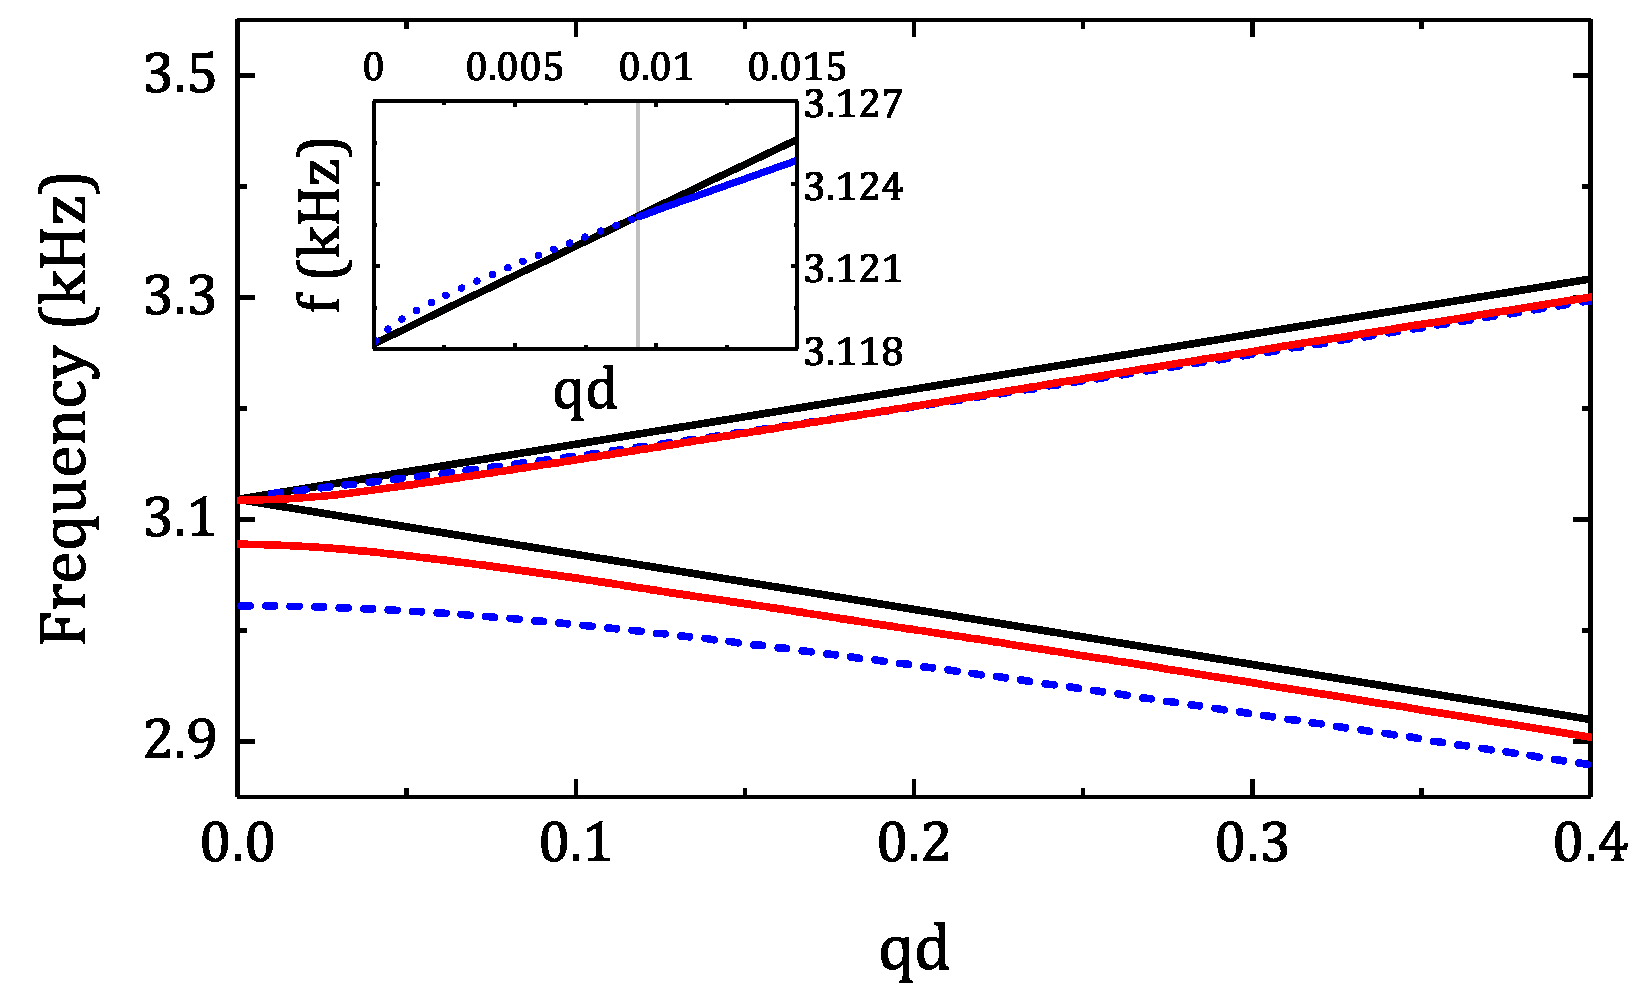
\includegraphics[width=0.8\linewidth]{asym_bandgap.eps}
\caption{Band structure of an~infinite periodic chain of shells in inviscid air environment. Solid black and red lines respectively show linear dispersion in air and dispersion calculated from \cref{eq:17Chain} (same as in \cref{fig:dispChain} (a)). Dashed blue lines show the~dispersion obtained from the~perturbation theory equations \cref{eq:BFChain} and \cref{eq:BGChain}. The~inset shows the~narrow region  $qd<q_cd \approx 0.01$ near the~$\Gamma$-point where the~upper band does not exist. The~leaky upper mode beyond $q=q_c$ is shown by blue line.}
\label{fig:asymgapChain}
\end{center}
\end{figure}


As for the~{\it upper} branch of the~dispersion curve, one may not treat $\Delta k_m$ as a~purely real value, so a~complex solution of \cref{eq:B15Chain} has to be found.
Since the~exponential decay with time is expected for all complex solutions, the~solution is restricted to the~lower part of the~complex plane, where $\im \Delta k_m = \im \omega/c_0 <0$.
However, the~right-hand-side of \cref{eq:B15Chain} remains to be purely imaginary, and therefore the~real parts of $(\Delta k_m - q)$ and $(\Delta k_m + q)$ need to have opposite signs.
This implies that the~term $(\Delta k_m - q)$ must lie in the~third quadrant, and the~term $(\Delta k_m + q)$ --- in the~fourth quadrant.
Because of that the~two inequalities $\re(\Delta k_m +q)>0$ and $\re(\Delta k_m -q)>0$ must be valid, which is achieved provided $|\re\Delta k_m| < q$.
The~latter condition cannot be satisfied when $q=0$, hence the~upper band never reaches the~$\Gamma$-point.
In \cref{eq:B15Chain}, the~first and the~second terms belong to the~third and the~first quandrants, respectively, given the~chosen branch cut along the~negative imaginary axis.
With that, I rewrite the~dispersion equation \cref{eq:B15Chain} using the~dimensionless variables $x=q/\kappa_m$ and $y= \Delta k_m/\kappa_m$ as
\begin{equation}
\label{eq:B16Chain}
\frac{1}{\sqrt{y-x}} = - 2i - \frac{1}{\sqrt{y+x}}.
\end{equation}
This equation can be squared and brought to a~biquadratic form over $x$, as both its left- and right-hand sides lie in the~same (third) quadrant.
After executing the~transformation mentioned one obtains:
\begin{equation}
\label{eq:B17Chain}
4 x^4 + x^2(1-8y^2-4y) + 4y^4 +4 y^3 =0.
\end{equation}
The~exact solution of this equation is not of much importance, whereas finding the~behavior of $y(x)$ in the~region of small $x$ and $y$ is crucial for understanding the~features of the~upper dispersion band.
The~series solution that satisfies \cref{eq:B17Chain} runs over integer powers of $(x/2)^{2/3}$:
\begin{equation}
\label{eq:B19Chain}
 y(x) \approx e^{-i\pi/3}\left(\frac{x}{2}\right)^{2/3} + \frac53 e^{i\pi/3}\left(\frac{x}{2}\right)^{4/3} + \left(\frac{x}{2}\right)^2, \,\,\,x << 1,
\end{equation}
which defines the~dispersion relation for the~upper branch to be
\begin{equation}
\label{eq:BGChain}
\omega(q)=\frac{2 \pi m c_0}{d}+ \Delta k_m c_0 \approx \frac{2 \pi m c_0}{d} + \kappa_m c_0 \left[e^{-i\pi/3}\left(\frac{q}{2\kappa_m}\right)^{2/3} + \frac53 e^{i\pi/3}\left(\frac{q}{2\kappa_m}\right)^{4/3} + \left(\frac{q}{2\kappa_m}\right)^2\right].
\end{equation}

This relation is valid for small wavevectors, $q << \kappa_m$.
Yet, the~group velocity appears to grow infinitely close to the~$\Gamma$-point, as $\partial \omega/ \partial q \propto q^{-1/3}$, which is not a~reasonable physical dependence here.
However, there is no contradiction, as it was previously established that the~condition $\re\Delta k_m < q$ must hold, which is numerically equivalent to $q>q_c \approx \kappa_m/20$.
The~latter indicates that within the~interval $0<q<q_c$, the~solution does not exist and thus the~mode does not propagate.
The~nonexisting part of the~band is shown by the~dashed line in the~insert to \cref{fig:asymgapChain} and is not visible in other figures, as the~region $0<q<q_c$ is extremely narrow.
It is peculiar that, unlike the~red-shifted lower band of the~doublet, the~upper branch is not blue-shifted as would be expected in the~nearly free electron model.
The~width of the~band gap is thus equal to
\begin{equation}
\label{eq:B20Chain}
\Delta f = \frac{c_0 \kappa_1}{2\pi} = \frac{c_0\left(z - \epsilon\right)^2}{2\pi^2 d},
\end{equation}
making the~gap opening strongly asymmetric.
The~gap width in the~presented perturbation theory is calculated to be $\Delta f \approx 100$ Hz for the~region near $3.1$ kHz.
This value is almost three times larger than the~numerically obtained value of only $35$ Hz (see \cref{fig:dispChain}).
The~observed mismatch arises from the~fact that the~small parameter of the~perturbation theory $z~=~\dfrac{\pi k a}{2}\dfrac{i Z_p}{\rho_0 c_0}$ is not actually small, being $z \approx 0.95$ near the~frequency $\omega = 2 \pi c_0/d$.
Even though the~ratio of impedances $iZ_p/\rho_0 c_0$ is small, it does not guarantee that the~parameter $z$ in the~series of the~perturbation theory is small as well, which results in poor estimation of the~band gap.
Nevertheless, the~developed perturbation theory qualitatively recovers the~asymmetry between the~two bands in the~doublet near the~$\Gamma$-point, and is therefore of principal importance.

In general, the~unusual structure of the~band gap is caused by the~two factors: the~cylindrical geometry of the~system and the~weakness of the~scattering, which is characterized by {\it imaginary} impedance $Z_p$.
Similar effects have been discovered for leaky surface acoustic and electromagnetic waves propagating along periodically corrugated surfaces \cite{maradudin2,maradudin3}.
The~band structures in these cases also feature the~asymmetric level repulsion and nonvanishing group velocity for the~upper band in the~doublet.
The~system described in this chapter exhibits the~same anomalies as the~systems with surface corrugations in \cite{maradudin2,maradudin3} since the~eigenvalue problem for the~periodic arrangement of shells in \cref{fig:geometryChain} requires expanding solutions over cylindrical functions, which is also the~case for the~surface modes being scattered by semi-cylindrical corrugations.

%The~asymmetric band opening and non-vanishing group velocity of the~upper band have been recently reported for leaky surface acoustic \cite{maradudin2} and electromagnetic \cite{maradudin3} modes propagating along periodically corrugated surfaces. The~eigenvalue problem for surface modes at the~surface corrugations, having cylindrical symmetry with axis along $z$, and the~eigenvalue problem for the~periodic set of cylinders in \cref{fig:geometryChain} require similar expansions over cylindrical functions. Due to this similarity the~spectra of leaky eigenmodes for these two geometries exhibit the~same anomalies.



\section{FEM Numerical Simulations}

\subsection{Transmission through the~Finite Chain}

%%%%%%%%%%%%%%%%%%%%%%%%
%%%%%%%%%%%%%%%%%%%%%%%%
%%%%%%%%%%%%%%%%%%%%%%%%

In order to obtain the~transmission properties of the~finite chain of perforated shells, I numerically solve the~set of equations \cref{eq:12Chain} for different number of scatterers $2N+1$ in the~chain.
The~transmission coefficient, defined as
\begin{equation}
T(f) = \frac{1}{2 N p_0 v_0} \int\limits_{-N d}^{N d} p_{tot}(d, y) v_{tot,x}^{*}(d, y)dy,
\end{equation}
is then calculated and visualized in \cref{fig:tr3141Chain}.
Here $p_{tot}(x,y)=p+p_{sc}$ and $v_{tot,x}(x,y)= -(i/\omega \rho_0) \partial p_{tot}/\partial x$ are the~the~total pressure and the~$x$-component of the~total velocity, respectively.
I calculate the~transmission spectrum for inviscid air (using \cref{eq:ZpIdealChain} as the~impedance of the~shells) and for air with its real viscosity (using \cref{eq:ZpChain}).
The~value of the~transmission coefficient is very close to one within a~wide range of frequencies, which agrees with the~numerical results reported in \cite{garcia1}.
Still, there is a~deep minimum around 3.1 kHz, and further I will show that it is caused by the~resonant coupling of the~incident sound with the~eigenmodes of the~chain.
Comparing viscous and inviscid cases, one concludes that the~deepness of the~minimum is reduced by viscosity, and the~resonance position is considerably red-shifted which is clearly visible in \cref{fig:tr3141Chain}.



\begin{figure}
\begin{center}
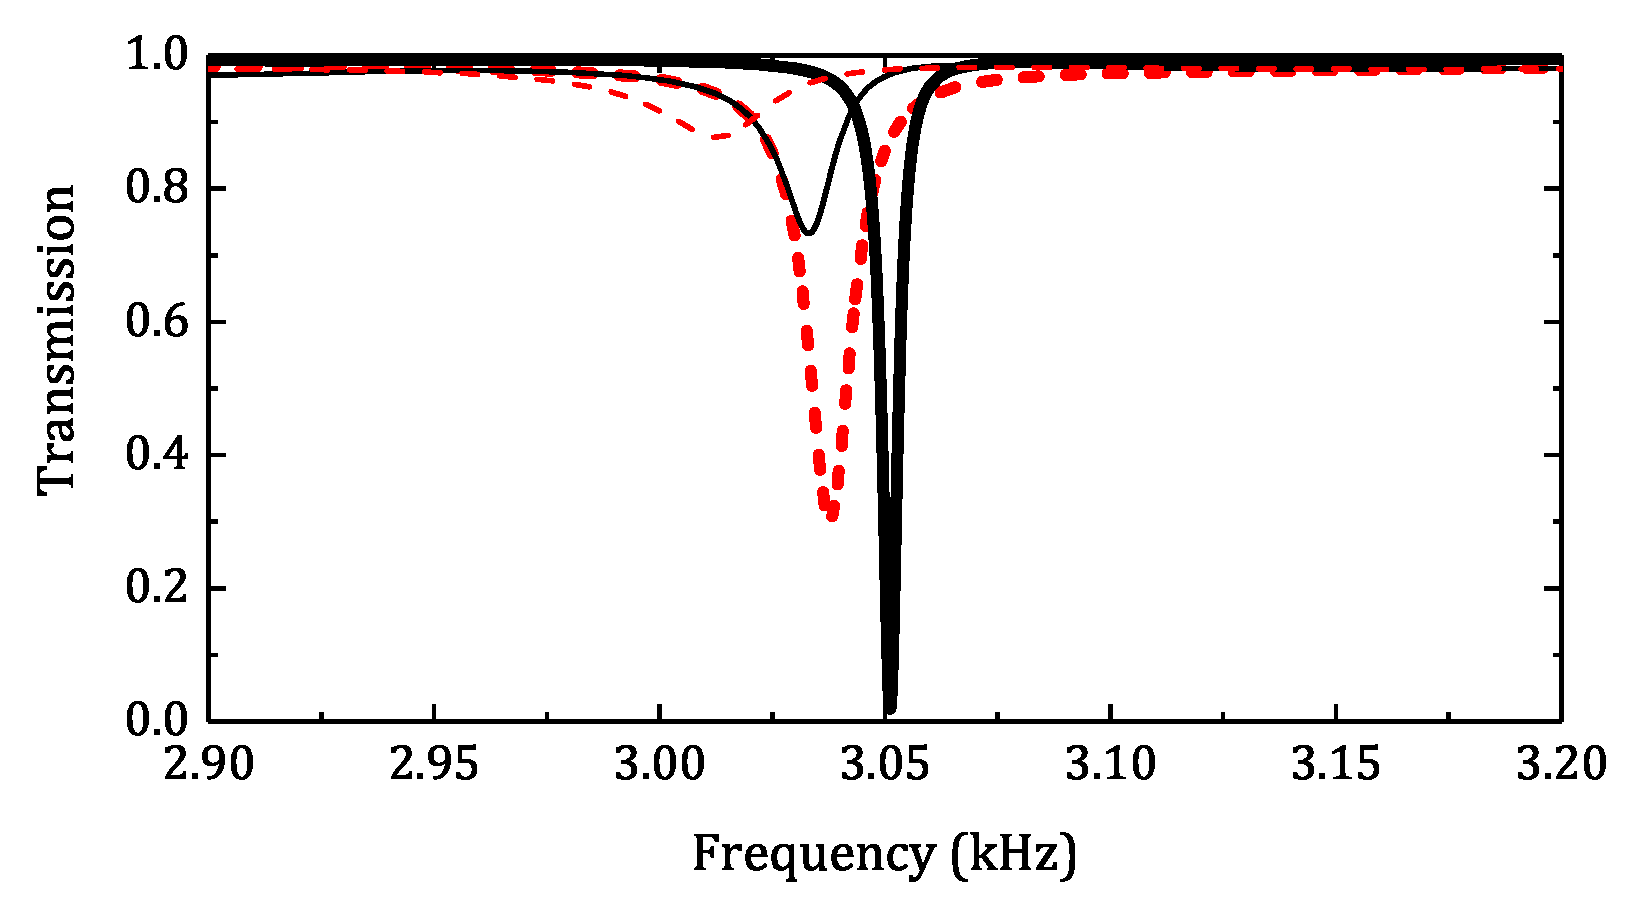
\includegraphics [width=0.9\linewidth]{tr_31_41.eps}
\caption{Transmission coefficient for the~chain of 31 (dashed red lines) and 41 (solid black lines) perforated shells. Results for inviscid and viscous air are shown by thick and thin lines respectively.}
\label{fig:tr3141Chain}
\end{center}
\end{figure}


\begin{figure}
\begin{center}
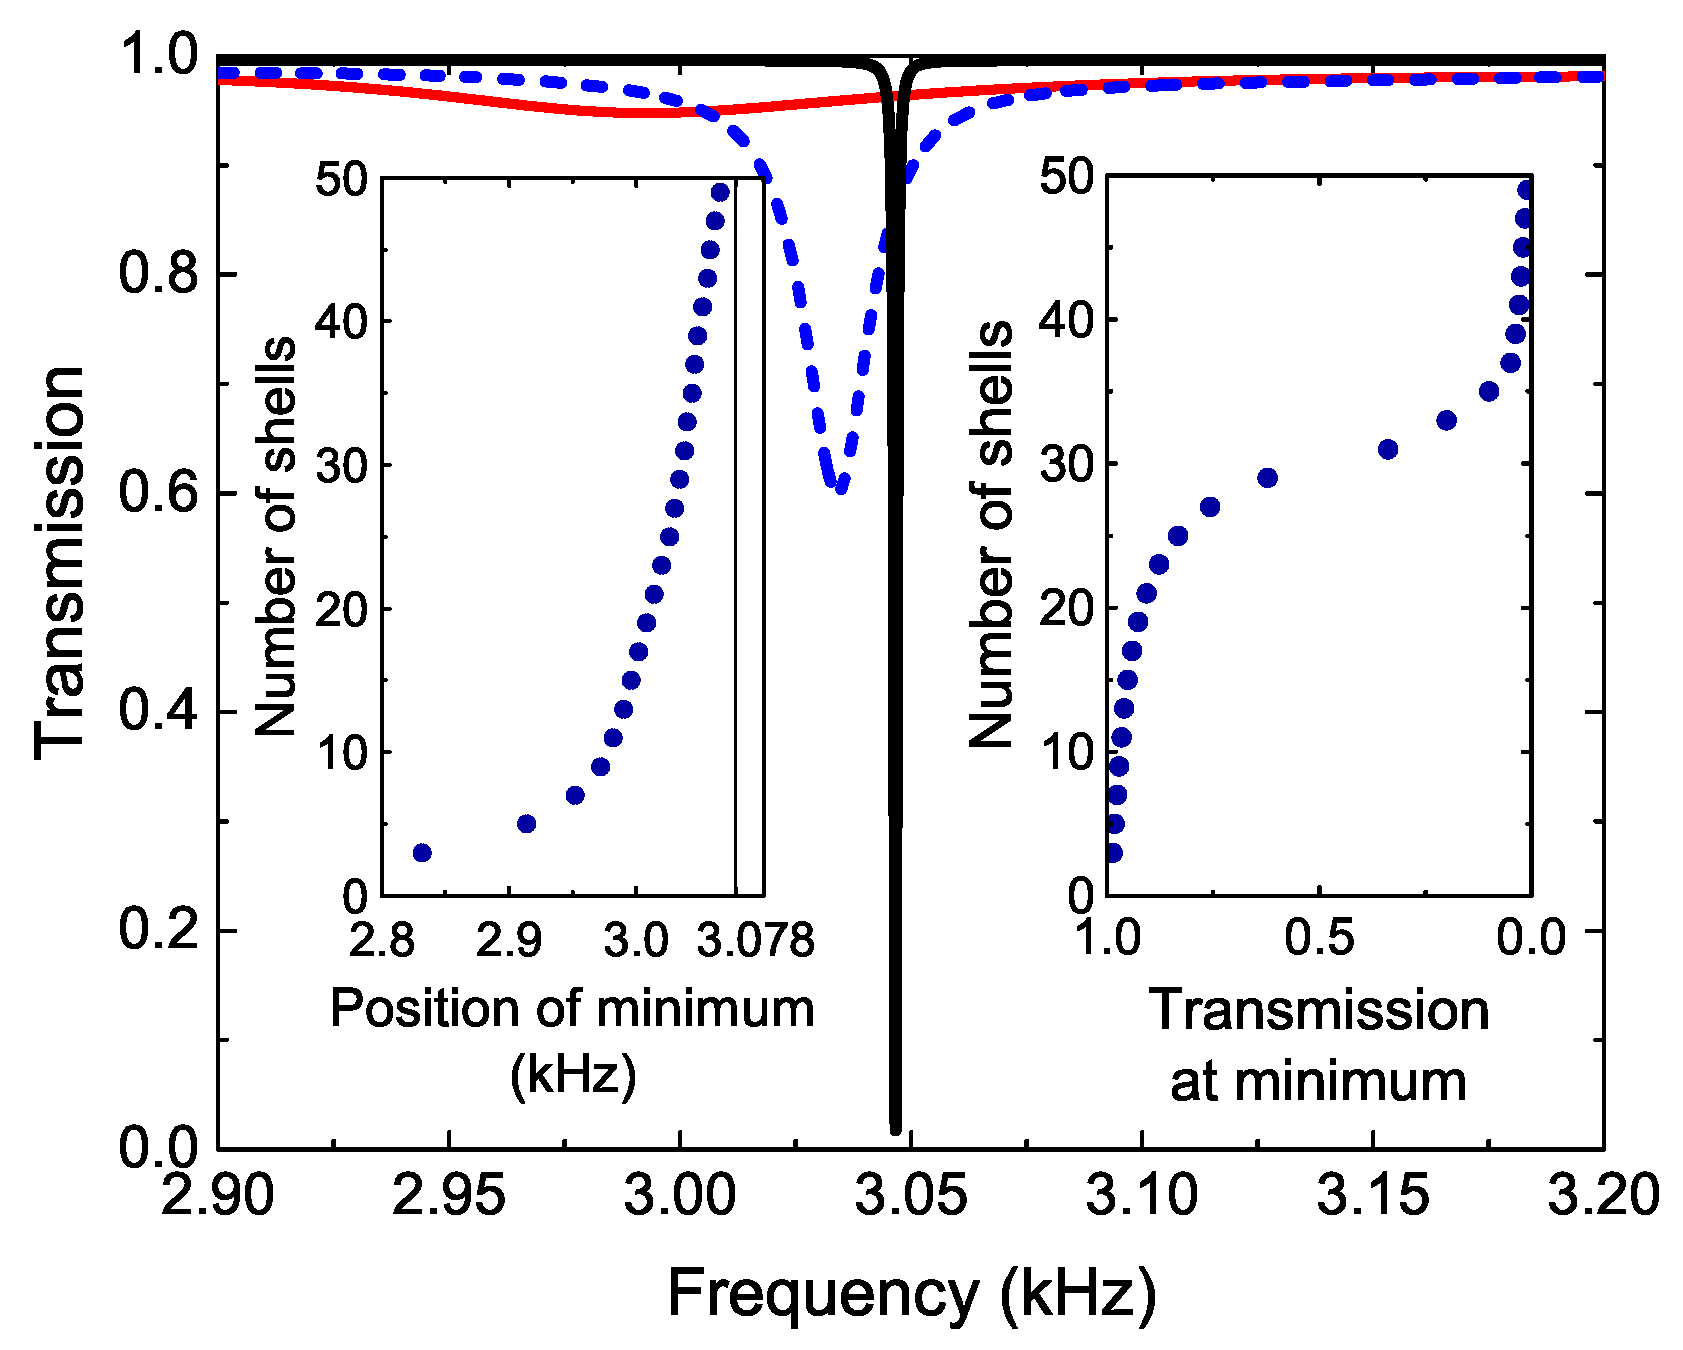
\includegraphics [width=0.7\linewidth]{tr_pos_num.eps}
\caption{Transmission coefficient for the~chain of 15 (solid red line), 29 (dashed blue line), and 37 (solid black line) perforated shells. Results are obtained for inviscid air. Inserts: position (left panel) of the~transmission minimum and its deepness (right panel) vs number of shells in the~chain.}
\label{fig:trposnumChain}
\end{center}
\end{figure}

Clearly, chains of perforated shells need to have sufficient length in order to establish the~spectrum of eigenmodes, as the~shells are weak scatterers.
Otherwise, one will not achieve any pronounced behavior of the~eigenmodes and therefore the~minima in transmission, if any, will be quite shallow.
Namely, even without the~viscosity in the~picture, there is hardly any visible minimum in the~transmission spectrum of a~15-unit chain, and it will completely disappear when the~viscosity is accounted for.
Increasing the~number of scatterers makes the~resonant minimum deeper and sharper, and also blue-shifts it.
For a~very long chain, the~minimum converges on a~specific position.
The~minima shown in \cref{fig:tr3141Chain} approach the~frequency of 3078 Hz as the~length of the~chain is increased.
This frequency, 3078 Hz, is the~first nonzero eigenfrequency at the~$\Gamma$-point in the~band structure of the~infinite periodic chain of shells in ideal air environment (see \cref{fig:dispChain}).
\cref{fig:trposnumChain} shows how the~deepness of the~resonant minimum and its position depend on the~number of units in the~chain.
It is interesting that the~position of the~resonance (left panel of \cref{fig:trposnumChain}) converges to 3078 Hz much slower than the~transmission at minimum (right panel of \cref{fig:trposnumChain}) approaches zero, making the~latter more sensitive to the~number of scatterers.


\subsection{Transmission through the~Infinite Chain}

Now, I will calculate the~transmission properties of the~infinite chain of scatterers, which requires solving the~set of equations \cref{eq:15Chain}.
In the~case of the~normal incidence of sound, the~transmission vanishes exactly at $f=3078$ Hz, which corresponds to the~frequency of the~lower level in the~doublet formed due to the~level repulsion (see \cref{fig:dispChain}(b)).
One can verify via numerical simulations that the~distribution of pressure over the~$y$-axis is symmetric (antisymmetric) for the~eigenmodes describing the~lower (higher) level of the~doublet.
It is known that an~external plane wave can only excite symmetric modes at normal incidence.
The~antisymmetric modes, in particular, the~upper level of the~doublet, cannot be excited in such geometry.
Such modes are commonly referred to as deaf modes \cite{jose,ward}.
Once the~symmetric mode in 1D chain of scatterers is directly excited, the~transmission is practically $100\%$ suppressed.
The~energy is then mostly reflected back (about 85$\%$), or equally redirected by $\pm 90^{\circ}$ towards both ends of the~chain (remaining 15$\%$).

\begin{figure}
\begin{center}
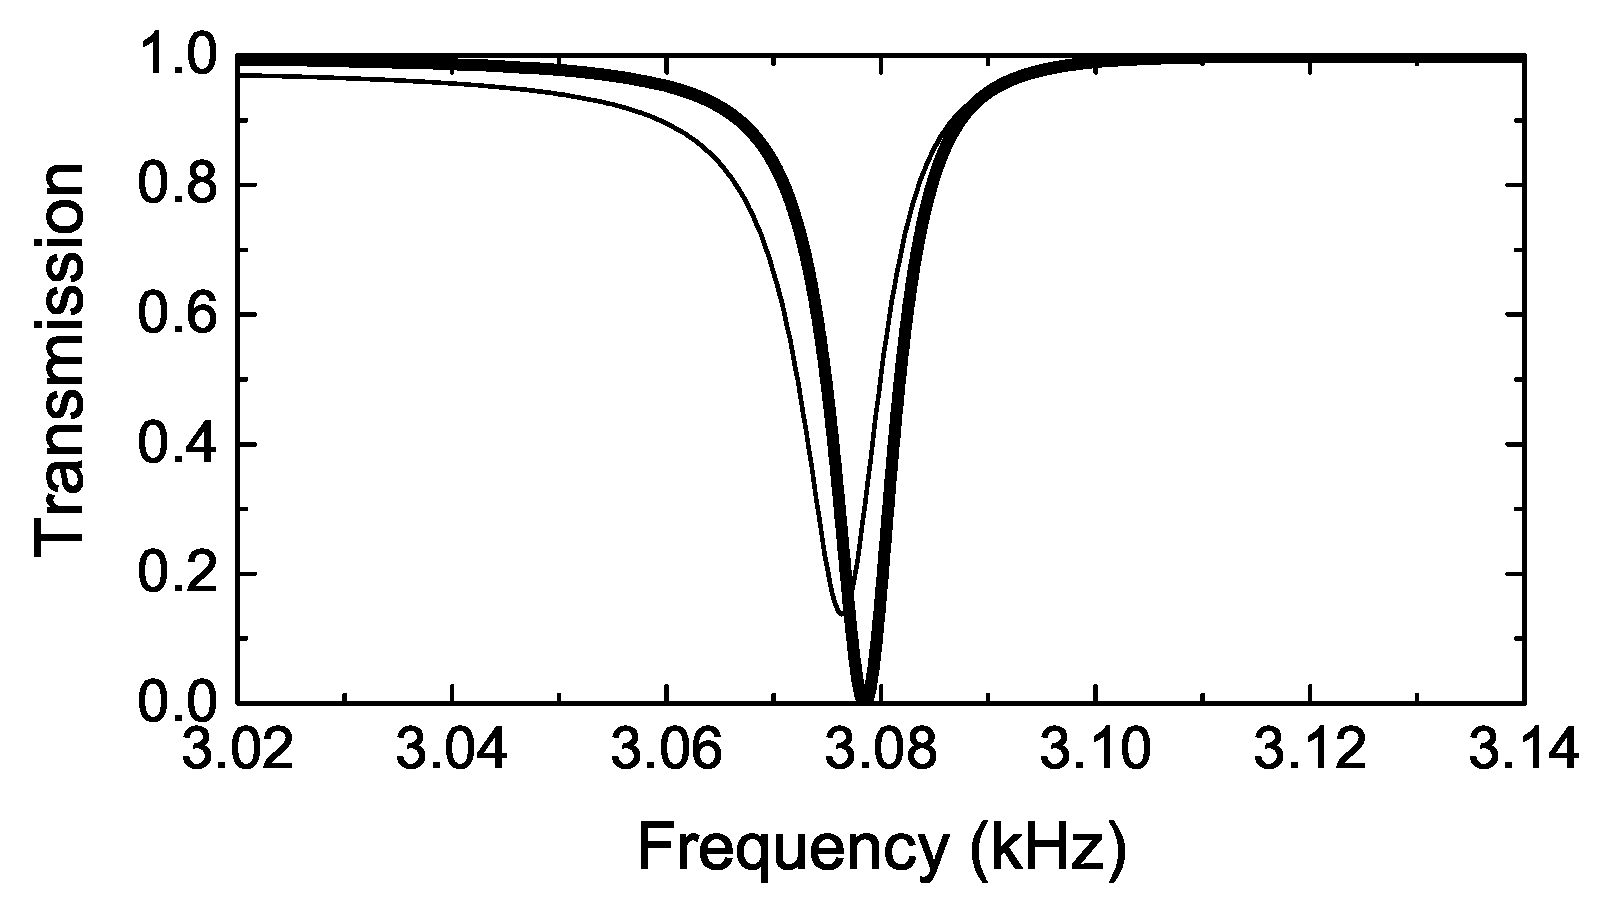
\includegraphics [width=0.7\linewidth]{tr_inf.eps}
\caption{Transmission spectrum of an~infinite chain of perforated cylindrical shells at normal incidence. Thick and thin lines are for inviscid and viscous air, respectively.}
\label{fig:trinfChain}
\end{center}
\end{figure}

Despite being a~deaf mode, an~antisymmetric mode may still be excited indirectly.
As was reported in \cite{norris1}, one may achieve the~effect of redirection of sound in a~sonic crystal of elastic rods due to the~Poisson-like effect.
Namely, the~incoming sound excited the~flexural modes of the~rods, and those modes coupled to the~antisymmetric deaf modes via evanescent modes. Such indirect excitation allowed only a~maximum of $46\%$ of acoustic energy to be reflected or redirected at the~frequency of the~mid-gap.

It is important to note from \cref{fig:trinfChain} that the~resonance in a~chain surrounded by viscous air is not significantly altered by dissipation, specifically, there is only a~slight red shift and almost no broadening of the~resonance (the~width remains approximately $\Delta f=30$ Hz).
As is seen from \cref{fig:tr3141Chain} and \cref{fig:trposnumChain}, the~most important factor defining the~shape of the~resonant minimum is the~length of the~chain.
The~viscosity is then does not qualitatively change the~observed phenomena, and only weakly contributes to the~quantitative results.
Due to viscosity, the~transmission at the~resonance does not reach zero and becomes finite.
Still, about $80\%$ of acoustic energy experiences either reflection or redirection as the~symmetric leaky modes of the~chain are excited.
%%
The~leaky modes are not proper spectral modes, and one benefits from this fact since such modes can be directly excited by external sound due to their interaction with the~environment.
Moreover, the~inequality $\im f \ll \Delta f \ll \re f$ holds, and for that reason the~resonant excitation is well established.


When the~external acoustic plane wave is incident at an~angle, there is no symmetry of the~incoming wave over the~$y$-axis, which makes the~excitation of both symmetric and antisymmetric eigenmodes possible.
For that reason, the~two minima appear in the~transmission spectra in \cref{fig:trangleChain}.
In order to find the~position of each minimum, the~wave vectors of the~incoming sound $\mathbf{k}$ and the~eigenmode $q$ must satisfy the~following relation:
\begin{equation}
\label{eq:18Chain}
k_{y}=(2\pi f/c_0) \sin \theta = q(f).
\end{equation}
The~latter condition, which requires matching of the~tangential components of the~wave vectors, is the~mathematical form of the~phenomenon known as the~Wood's anomaly \cite{maystre}.
As an~example, the~resonant minimum in the~transmission spectrum \cref{fig:trinfChain} can be considered as a~Wood's anomaly since at the~resonant frequency 3078 Hz, the~wavelength of sound in air is 11.1 cm, which closely matches the~period of the~chain $d=11$ cm \cite{garcia1}.
In the~reduced zone scheme, the~condition \cref{eq:18Chain} can be satisfied for multiple frequencies, depending on the~angle of incidence $\theta$.
For normal incidence, $\theta=0^{\circ}$, the~corresponding value of the~wave vector is $q=0$, which formally enables any dispersion band to be excited by external sound.
Together with the~symmetry consideration one concludes that normal incidence only triggers excitation of lower levels of the~doublets at the~$\Gamma$-point.

In general, \cref{fig:dispChain} shows the~points of crossing of the~straight dashed lines given by $q=2\pi f \sin\theta/c_0$ with the~dispersion bands, where the~condition \cref{eq:18Chain} is satisfied.
The~three dashed lines correspond to the~angles of incidence $\theta = 5^{\circ}$, $\theta = 10^{\circ}$ and $\theta = 15^{\circ}$.
For $\theta = 5^{\circ}$, the~first two crossings occur at $f \approx 2.85$ kHz and $f \approx 3.40$ kHz.
Consequently, the~transmission minima in \cref{fig:trangleChain} are observed near these frequencies.
These two minima are separated by the~interval of about 550 Hz, which is significantly larger than either the~width of each minimum or the~width of the~doublet at the~$\Gamma$-point.
The~latter fact makes each minimum well-resolved, and is explained by the~difference in the~dispersion of the~two bands.
Since the~upper (antisymmetric) and the~lower (symmetric) bands are the~continuations of the~doublet levels at the~$\Gamma$-point, they exhibit normal and anomalous dispersion, respectively, meaning the~separation between their respective eigenfrequencies is increased away from the~$\Gamma$-point.


\begin{figure}
\begin{center}
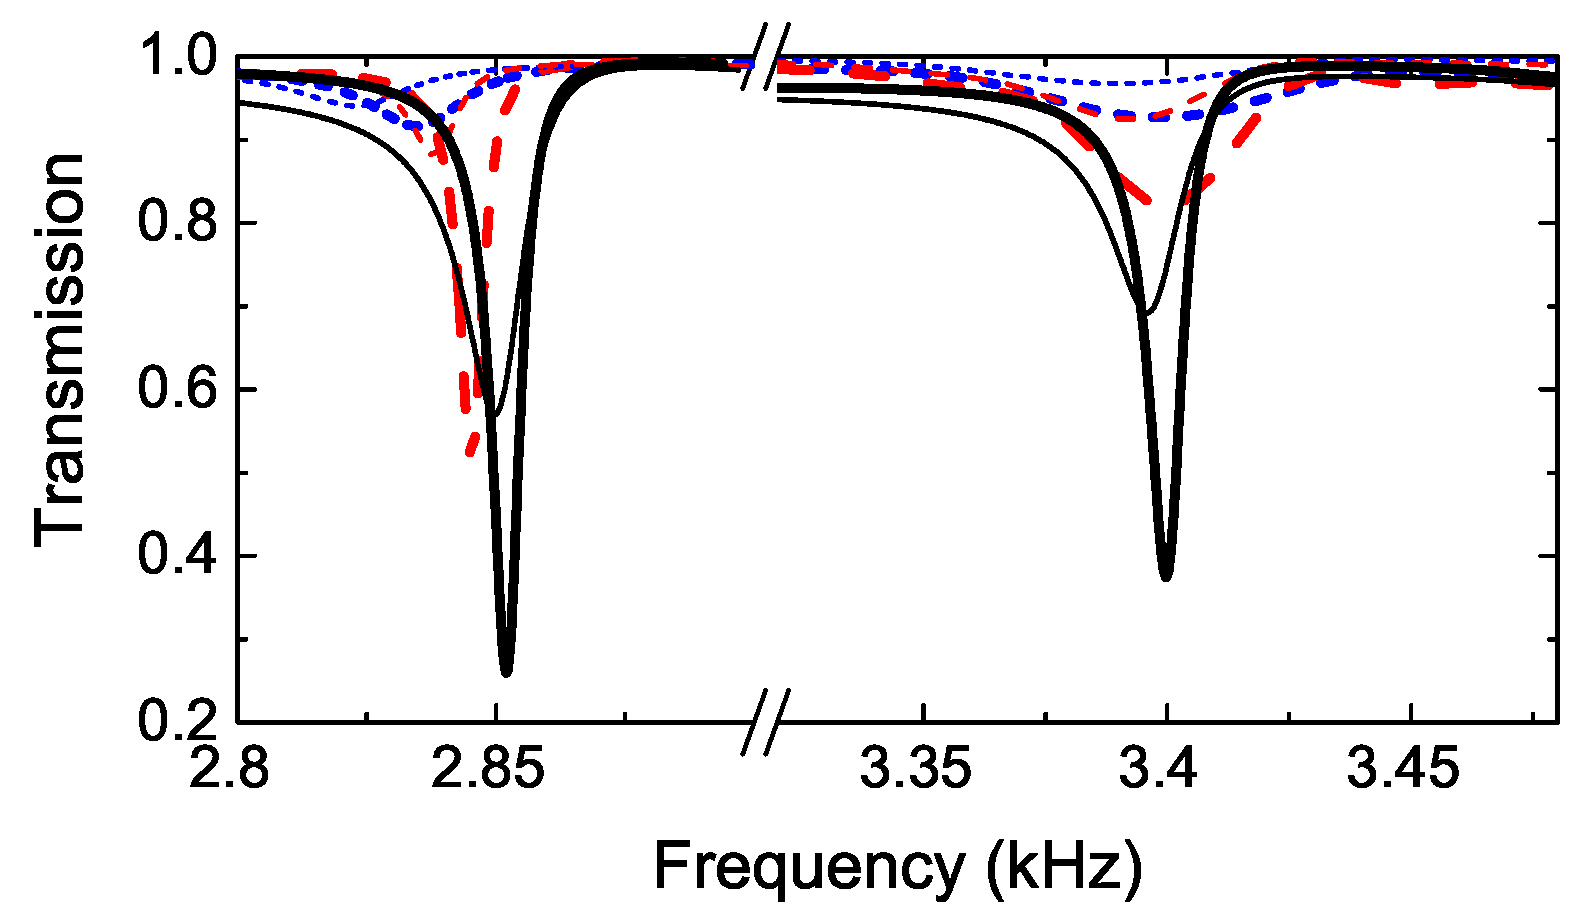
\includegraphics [width=0.7\linewidth]{tr_angle5.eps}
\caption{Transmission spectrum at oblique incidence, $\theta = 5^{\circ}$. Blue short-dashed, red long-dashed, and black solid lines are for the~chains containing 61, 121, and infinite number of cylindrical shells, respectively. Thick and thin lines show the~results for inviscid and viscous air. Note that two resonances are separated by $\approx 550$ Hz in frequency (compare to the~doublet width $35$ Hz).}
\label{fig:trangleChain}
\end{center}
\end{figure}


An~interesting anomaly arises in the~scattering of sound by the~chain of perforated shells as a~result of the~bands having different dispersion.
One can see that the~direction of the~phase velocities for both eigenmodes is the~same as the~direction of the~wave vector ${\bf q} = q\hat{y}$.
The~group velocity, however, acquires its sign from the~slope of the~corresponding band curve, so for the~lower band it is opposite to $\bf q$.
As the~group velocity points in the~direction of the~energy flow, it appears that the~scattering of the~incoming wave occurs in the~"wrong" direction.

\cref{fig:polarUChain} and \cref{fig:polarDChain} visualize the~angular distribution of intensity of scattered sound for the~angle of incidence $\theta = 5^{\circ}$.
In \cref{fig:polarUChain}, the~frequency of 3.40 kHz is selected for the~incoming wave to allow coupling with the~upper dispersion band (see \cref{fig:dispChain}).
The~scattered sound propagates almost exclusively in the~direction of the~parallel component $k_{y}\hat{y}$ of the~wave vector in the~incoming wave, due to the~normal dispersion of the~band.
In contrast with that, the~scattering at the~frequency of $f=2.85$ kHz, where the~matching condition \cref{eq:18Chain} holds for the~lower band with anomalous dispersion, occurs in the~direction against $k_{y}\hat{y}$ and produces anomalous pattern for the~scattered field (see \cref{fig:polarDChain}).

Both \cref{fig:polarUChain} and \cref{fig:polarDChain} also show the~results obtained for viscous air by green dashed lines.
Due to viscosity of air, the~scattered sound is of lower intensity in all the~directions.
Despite that, the~coupling to the~eigenmodes remains effective, and the~spikes of intensity in the~normal and "wrong" directions remain well-pronounced.


\begin{figure}
\begin{center}
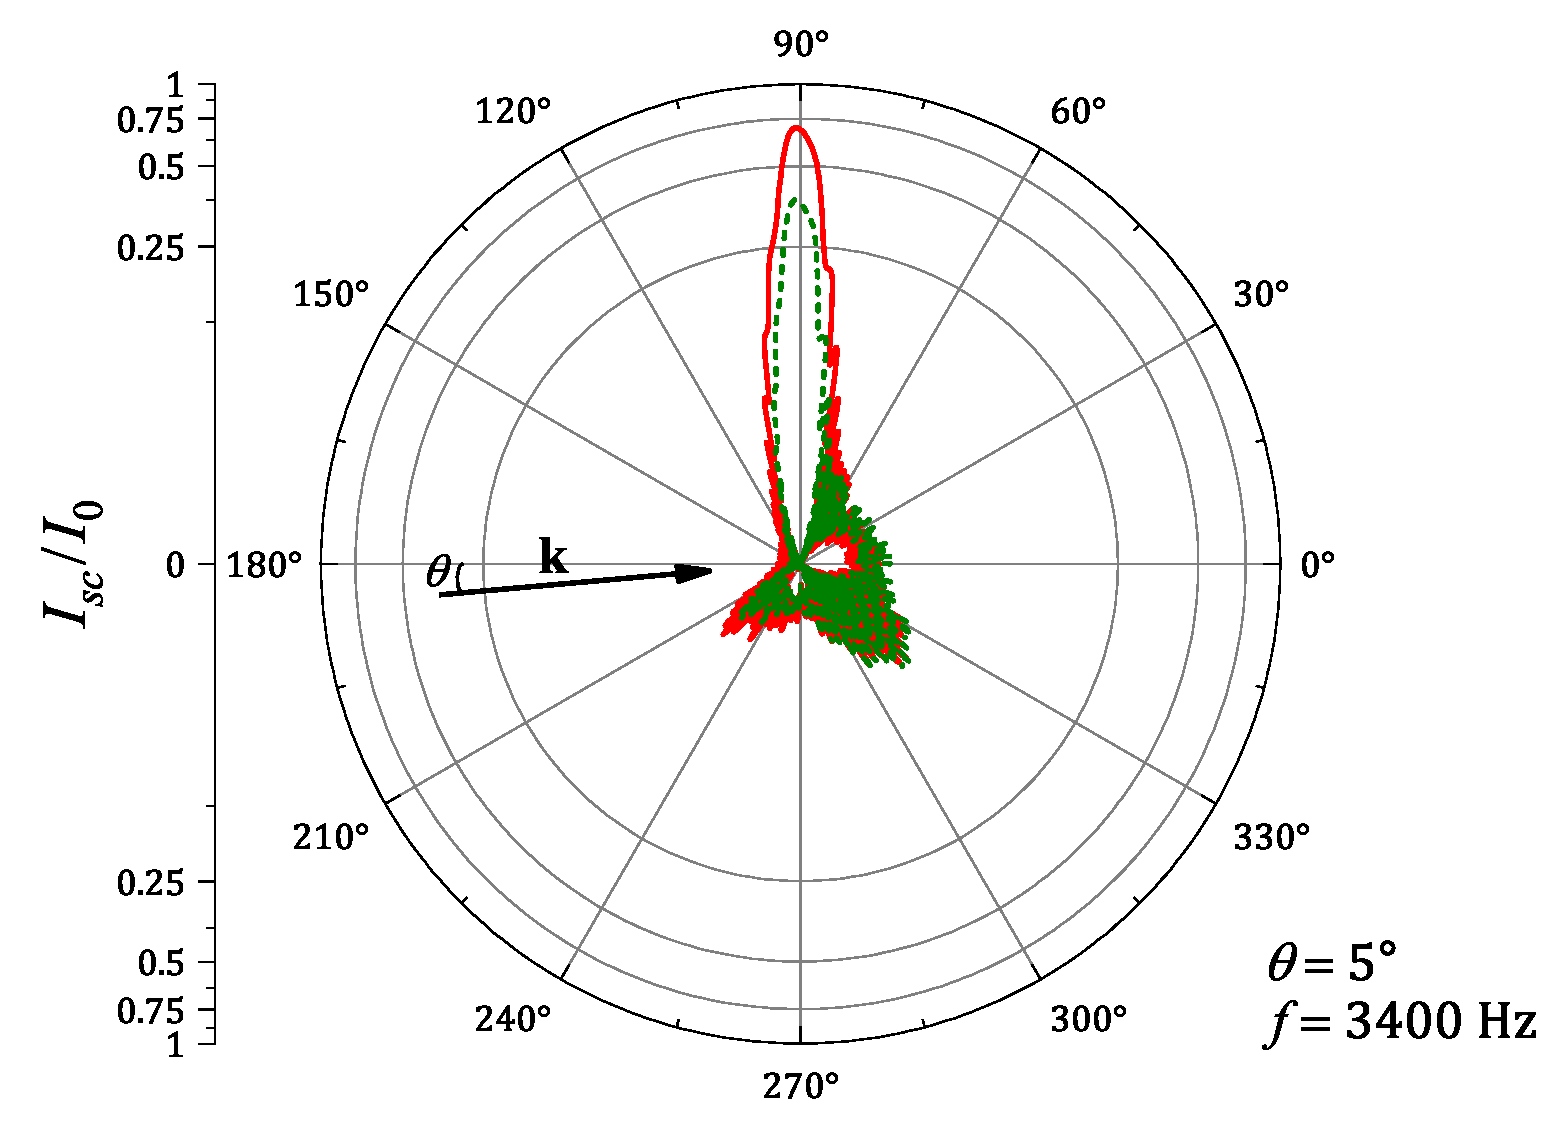
\includegraphics [width=0.9\linewidth]{polar_3400.eps}
\caption{Polar diagram showing distribution of intensity of scattered sound of frequency $f = 3400$ Hz (upper band in the~doublet having normal dispersion). Solid-red and green-dashed lines are for inviscid and viscous air, respectively. Black arrow shows the~direction of the~incident wave. An~essential part of scattered sound wave propagates along the~chain in the~direction of the~wave vector $\bf k_{\|}$. Note logarithmic scale along radius.}
\label{fig:polarUChain}
\end{center}
\end{figure}



\begin{figure}
\begin{center}
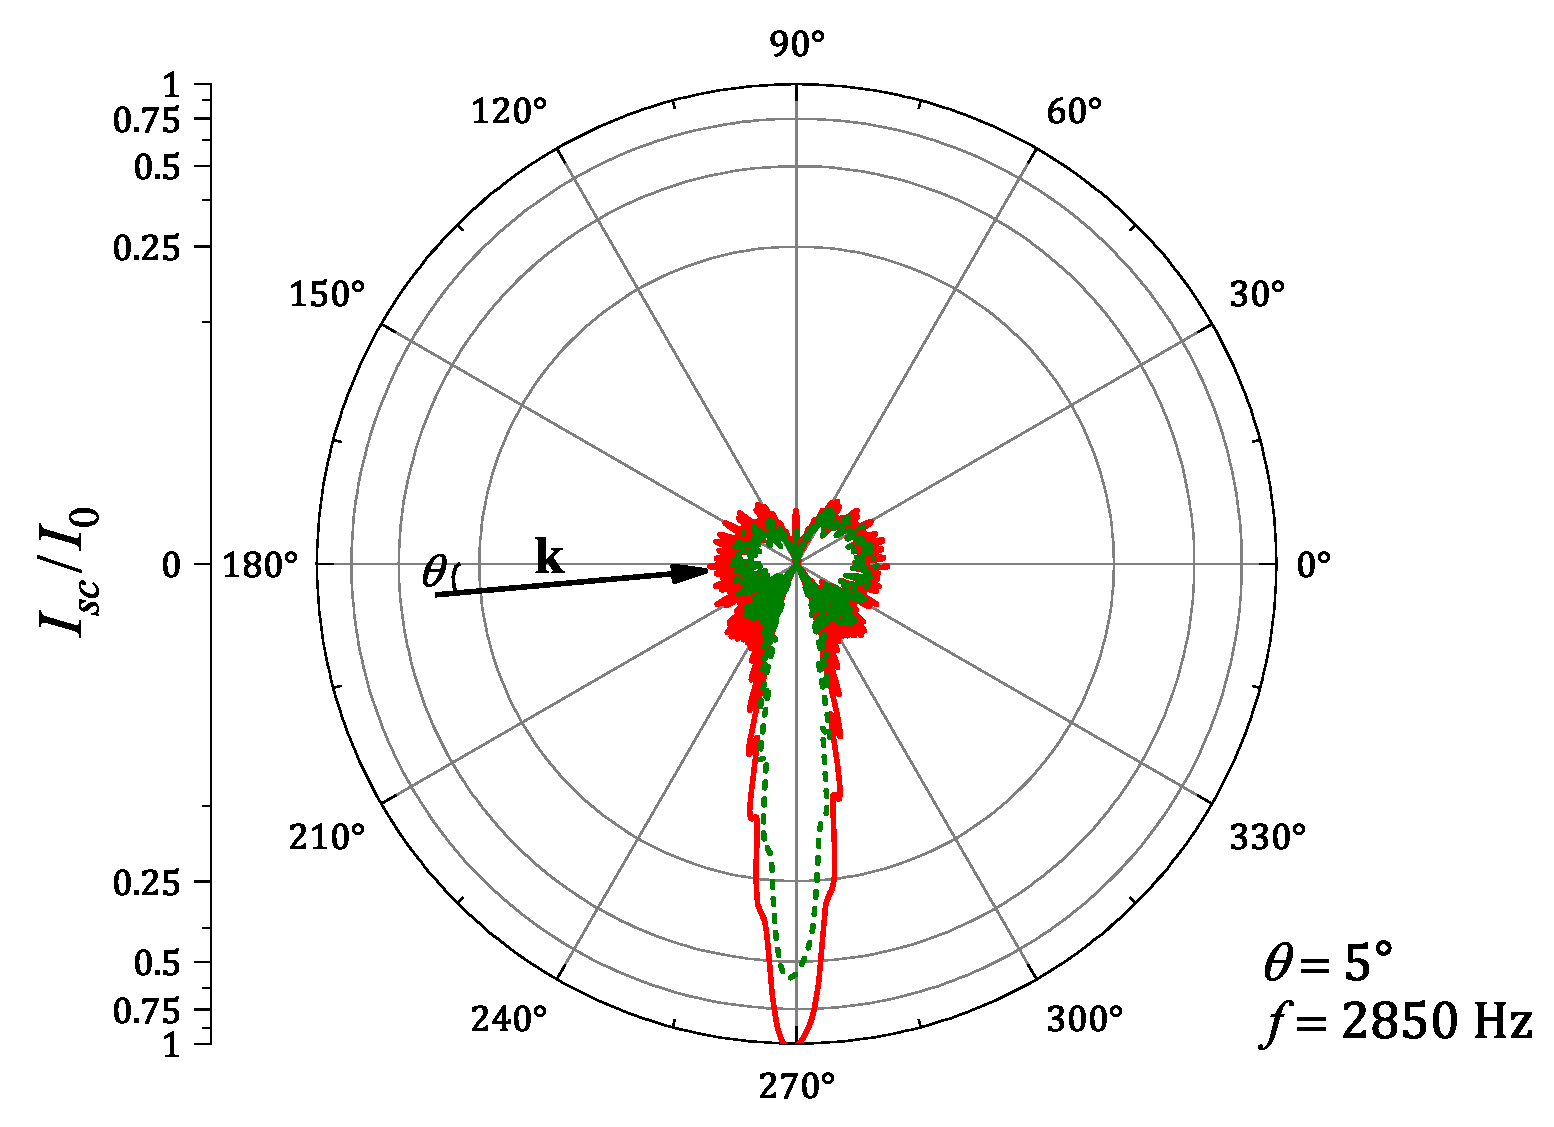
\includegraphics [width=0.9\linewidth]{polar_2850.eps}
\caption{The~same as in \cref{fig:polarUChain} but for the~frequency $f=2850$ Hz, corresponding to the~lower band of the~doublet, having anomalous dispersion. In this case the~scattering occurs in the~"wrong" direction, i.e., opposite to $\bf k_{\|}$.}
\label{fig:polarDChain}
\end{center}
\end{figure}


\begin{figure}
\begin{center}
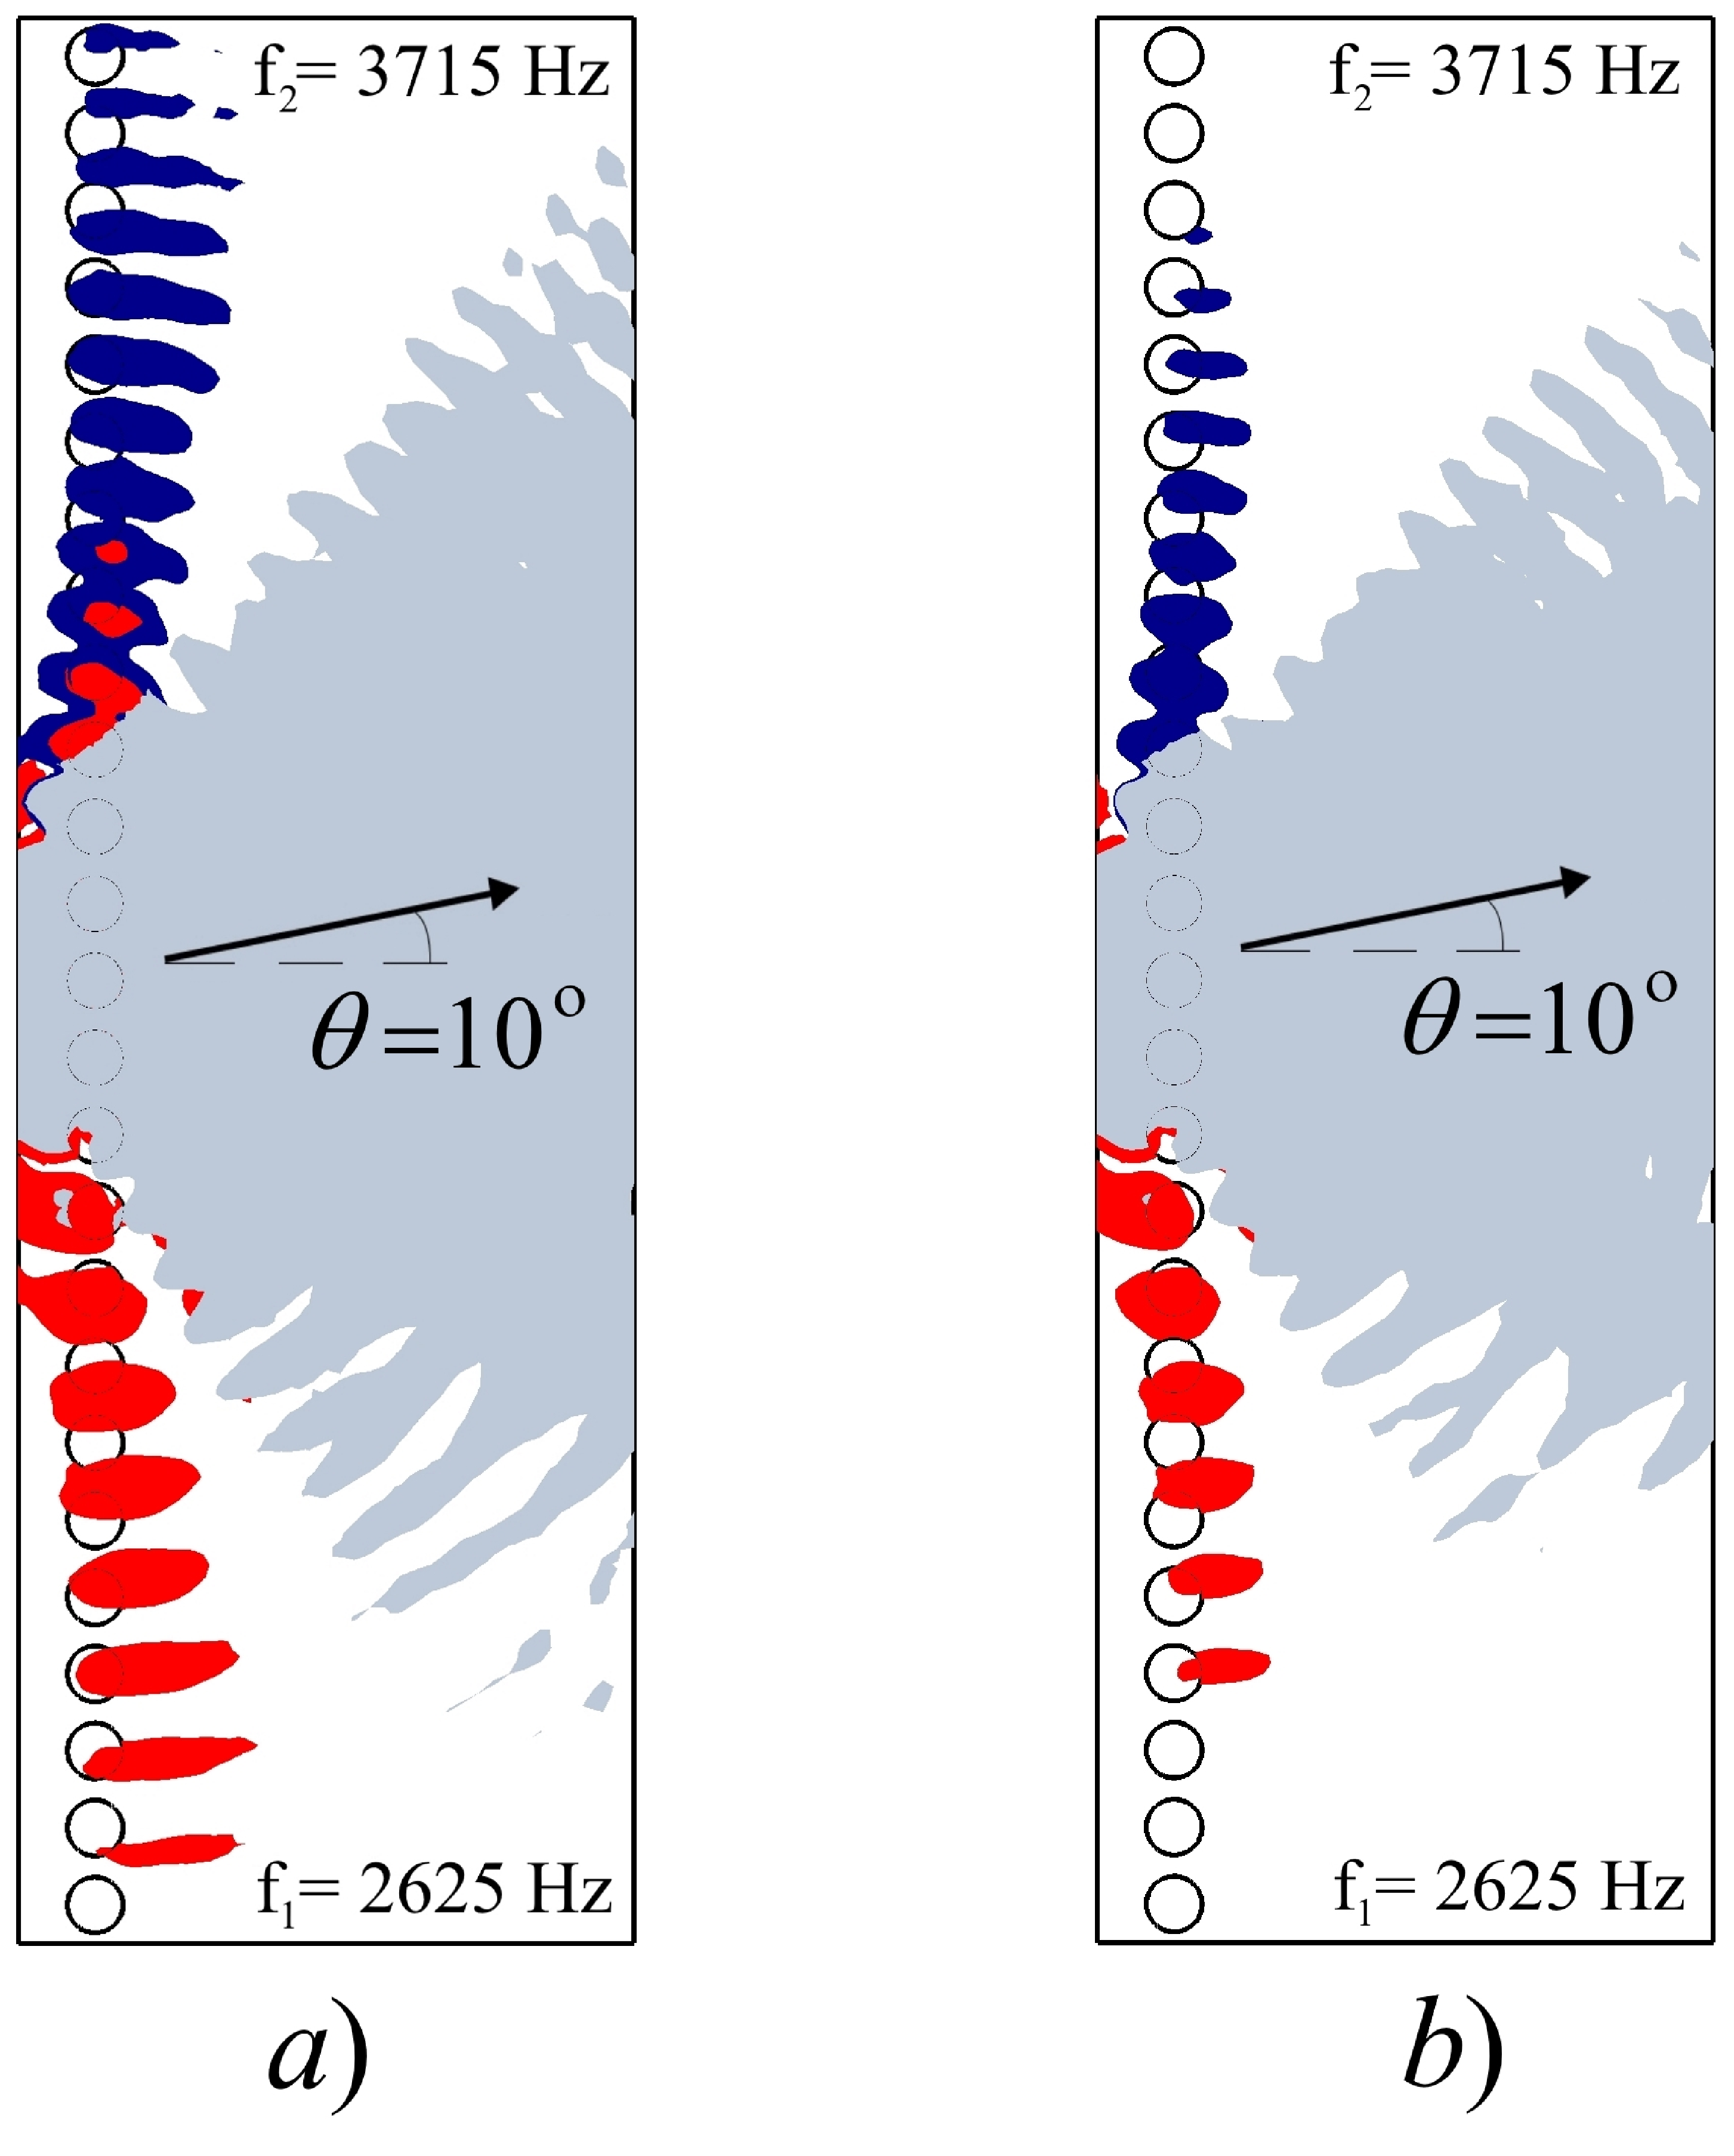
\includegraphics [width=0.7\linewidth]{bifreq_split.eps}
\caption{Distribution of intensity of a~bi-frequency signal (with $f_1=2625$ Hz and $f_2=3715$ Hz) transmitted through a~chain of 25 perforated shells. The~angle of incidence is $10^{\circ}$ and the~background air is inviscid (a) and viscous (b). The~central part of the~diffraction pattern (shown in grey) is a~mixture of two sound waves with frequencies $f_1$ and $f_2$.  The~red and blue fringes are the~split monochromatic components. The~low-frequency component (red) exhibits anomalous scattering, propagating against the~"natural" direction. The~high-frequency component (blue) follows the~"natural" direction due to its normal dispersion.}
\label{fig:bifreqChain}
\end{center}
\end{figure}


There is no great difference between the~intensities of the~normal and anomalous scattering for the~angles of incidence $\theta \geq 5^{\circ}$.
The~results in \cref{fig:trinfChain} serve as the~evidence for the~latter claim, showing that the~values of the~transmission coefficients in the~minima differ by $10\%$, with the~lower-frequency minimum being deeper.
For smaller angles $\theta$, however, the~eigenmode with normal dispersion produces much weaker minimum as it becomes a~deaf mode towards $\theta = 0^{\circ}$, and as a~result the~anomalous scattering dominates.
When $\theta \rightarrow 0^{\circ}$, the~frequency interval between two resonant minima in the~transmission spectra approaches the~width of the~doublet, which may be hard to see from the~plots as the~minimum corresponding to normal scattering vanishes completely.

The~plots in \cref{fig:trinfChain}-\cref{fig:polarDChain} clearly demonstrate the~effect of redirection of incoming sound by an~angle of about $90^{\circ}$.
This becomes possible in a~chain of weak scatterers when the~frequency and the~angle of incidence satisfy the~matching condition \cref{eq:18Chain}.


\subsection{Splitting of Acoustic Signal}

Additionally, the~chain of perforated shells may serve as a~splitter of a~bi-frequency acoustic signal.
Let us consider an~acoustic beam which is created by mixing two monochromatic sound waves and is incident on the~chain at a~certain angle $\theta$.
The~described beam will produce two monochromatic signals propagating along the~chain in the~opposite directions, provided that both frequencies of its components are solutions of \cref{eq:18Chain}.
In the~case of almost normal incidence, the~detuning between the~components needs to be much smaller than their frequencies (such bi-frequency signal is called a~beat).
Due to closeness to the~$\Gamma$-point, the~redirection of the~high-frequency component is suppressed and the~overall efficiency of splitting is reduced.

In \cref{fig:bifreqChain}, a~bi-frequency signal is incident at an~angle of $10^{\circ}$ on the~finite-length chain containing 25 perforated shells.
The~two monochromatic components of the~signal have frequencies of $2625$ Hz and $3715$ Hz, respectively, which are the~frequencies of the~two eigenmodes of the~chain that can be excited by the~wave incident at $10^{\circ}$ (see \cref{fig:dispChain}).
A~substantial part of acoustic energy propagates through the~chain, as the~angle of incidence is not very small and the~number of shells is not very large.
Nevertheless, one can observe a~clear pattern of split fringes towards either end of the~chain, for both ideal (\cref{fig:bifreqChain}a) and viscous (\cref{fig:bifreqChain}b) air.

The~chain of perforated shells, being a~purely mechanical system, demonstrates quite good efficiency of splitting.
The~amounts of energy that are converted into the~low-frequency component, propagating down (anomalous scattering), and high-frequency component, propagating up (normal scattering), are as high as $8\%$ ($5\%$) and $10\%$ ($7\%$), respectively, for the~chain in ideal (viscous) air environment.
%In \cref{fig:bifreqChain} we show the~splitting of a~bi-frequency signal when it hits the~chain at the~angle of $10^{\circ}$ in ideal (panel (a)) and viscous (panel (b)) air. The~frequencies of the~monochromatic components, $2625$ Hz and $3715$ Hz, are obtained from the~band diagram in \cref{fig:dispChain}. Since the~chain contains only 25 shells and the~angle of incidence is not very small, the~essential part of acoustic energy propagates directly through the~chain. Nevertheless, a~clear pattern of split fringes is observed even for viscous air.
%The~efficiency of splitting is quite good for a~pure mechanical splitter, for ideal (viscous) air $8\%$ ($5\%$) of energy is converted into the~low-frequency component, propagating down (anomalous scattering) and $10\%$ ($7\%$) of energy is converted into the~higher-frequency component, propagating up (normal scattering).



%++++++++++++++++++++
\section{Summary}

This chapter presents a~rigorous study of the~interaction between the~acoustic waves and the~periodic chain of thin perforated cylindrical shells, which results in redirection and splitting of incident sound.
The~problem of diffraction of sound by the~periodic arrangement of shells is solved analytically in impedance approximation, applicable for situations with both ideal and viscous background fluid.
The~transmission coefficient is calculated for infinite and finite-length chains within a~wide range of frequencies, and agrees well with earlier numerical and experimental results reported in \cite{garcia1} and further expanded in \cite{victorthesis}.

To gain more insights into the~predicted phenomena, the~dispersion equation for the~infinite periodic chain is derived, and the~eigenmodes are then numerically obtained for aluminum scatterers in air.
Weak coupling between the~scatterers and sound causes the~eigenmodes to be leaky modes, propagating with phase velocity close to the~speed of sound in air and slowly radiating energy away from the~chain.
The~eigenmodes can be resonantly excited by the~incident sound, leading to sharp minima in the~transmission spectrum at the~frequencies satisfying specific matching condition.

At normal incidence, the~coupling of a~monochromatic acoustic wave is only possible to the~symmetric chain eigenmode, which results in a~single deep minimum in the~transmission.
The~antisymmetric mode, no matter how close to the~symmetric mode frequency-wise, cannot be excited via normal incidence.
With this, equal parts of the~incoming sound are redirected in both directions along the~chain.

When the~incidence is oblique, the~external wave can couple to both symmetric and antisymmetric modes, and that causes two deep minima to appear in the~transmission spectrum.
These minima are well-resolved even for viscous air.
Since the~symmetric and antisymmetric modes exhibit anomalous and normal dispersion, respectively, the~anomalous scattering is strongly manifested in the~system.
The~scattering of acoustic energy along the~chain in the~opposite direction with respect to the~direction of incidence is shown to be a~strong effect, caused by the~resonant coupling between the~external sound and the~symmetric mode.
Consequently, the~chain of perforated scatterers can effectively serve as a~sound splitter.
Namely, a~sound beam consisting of two (or more) monochromatic components, which match the~frequencies of symmetric and antisymmetric modes and thus have different dispersion, is split into two parts propagating in opposite directions along the~chain.

In order to back the~theoretical predictions, one needs to perform further experimental work focused on designing and testing devices for filtering and splitting of sound waves at selected frequencies.


%In summary, we have demonstrated redirection and splitting of sound waves impinging a~periodic chain of thin perforated cylindrical shells.
%These conclusions have been obtained using an~analytical approach to the~problem of diffraction of sound by a~periodic chain of perforated cylindrical shells, which has been developed here.
%Scattering at the~shells is described in impedance approximation, which is applicable for both lossless and viscous background fluid.
%The~dispersion equation for the~eigenmodes of an~infinite periodic chain is derived and its complex solutions are obtained numerically for aluminum perforated shells in air.
%Since these shells are only weak scatterers of sound, the~eigenmodes are leaky waves propagating with phase velocity close to the~speed of sound in air, and they slowly decay due to dissipation and radiation.
%The~transmission coefficient is calculated for infinite and finite-length chains within a~wide range of frequencies.
%At normal incidence, the~coupling to the~lowest symmetric eigenmode gives rise to a~deep minimum in the~transmission.
%In this geometry, the~antisymmetric mode, which is close in frequency, is not excited and the~incoming wave is equally redirected along the~chain in both directions.
%At oblique incidence, the~external wave can be coupled to both symmetric and antisymmetric modes that leads to two deep minima in the~transmission spectrum which are well-resolved for viscous air.
%Here anomalous scattering is strongly manifested because the~symmetric mode exhibits anomalous dispersion while for the~antisymmetric one the~dispersion is normal.
%We find that resonant coupling of external sound to the~symmetric mode results in strong scattering  of acoustic energy along the~chain in the~"wrong" direction with respect to the~direction of incidence. Finally, we show that due to different dispersion of symmetric and antisymmetric modes a~sound beam consisting of two (or more) monochromatic components can be effectively split into two parts propagating in opposite directions along the~chain.
%Each part is a~monochromatic wave with the~frequency resonating with either symmetric or antisymmetric eigenmode.
%Further experimental work should be performed in order to support our theoretical predictions, which foresee useful devices for the~filtering and splitting of sound waves at selected frequencies.




%%% Local Variables: 
%%% mode: latex
%%% TeX-master: "dissertation"
%%% End: 

%%%%%%%%%%%%%%%%%%%%%%%%%%%%%%%%%%%%%%
\chapter{EFFECTS OF THE EPSILON-NEAR-ZERO TRANSITION LAYER ON THE PROPAGATION OF SURFACE PLASMON POLARITONS}


%%%%%%%%%%%%%%%%%%%%%%%%%%%%%%%%%%%%%%
\section{Introduction}

A~system consisting of dielectric and conducting regions can support a~specific type of electromagnetic excitations --- surface plasmon polaritons (SPPs), --- that are inherently confined in the~vicinity of the~interface between the~two media.
Such excitations propagate in a~self-sustainable manner, where the~electromagnetic field impinging the~conductor (usually a~metal) accelerates the~charges below the~the~metallic surface, and in their turn, the~oscillating charges emit the~coherent radiation back into the~dielectric.
The~amplitudes of both the~charge and the~field oscillations decay exponentially away from the~interface, and for that reason the~SPPs are extremely sensitive to the~surface conditions.
The SPPs find applications in a large number of areas of research and technology, ranging from optoelectronic devices and near-field imaging to tumor treatment and solar cell design \cite{smallworld,notsosmall,schuller}.

The~emergence of metamaterials allowed realization of unconventional material properties in physical devices, which led to the~observation of quite unique electromagnetic phenomena such as, for example, negative index of refraction \cite{veselago,pendry,shalaev2}.
Besides the~possibilities to achieve negative dielectric permittivity and/or magnetic permeability, metamaterials can be engineered to create regions where the refractive index is almost zero \cite{schilling}.
The latter manifests in either sophisticated metal-dielectric compounds or, what is more surprising, even in systems built from the dielectric materials only \cite{moitra}.

While the propagation of electromagnetic waves through such epsilon-near-zero (ENZ) regions has been studied to a certain extent \cite{ginzburg}, it is still of great interest to study the corresponding behavior of the surface plasmons.
Moreover, I will explain in this chapter that a thin ENZ layer always emerges at any metal-dielectric interface which thus qualitatively modifies the SPP properties.
Consequently, one will be able to tune the plasmonic properties by applying an external electrostatic field to the transition layer and thus gaining control over its width.

%%%%%%%%%%%%%%%%%%%%%%%%%%%%%%%%%%%%%%%%%%%%%%%%%%%%%%%%%%%%%%%%%%%%
\section{Metal-Dielectric Interface}

In the~simplest case of the~SPP propagation along the~planar metal-dielectric interface, one typically views the~two media as perfectly uniform materials, with the~boundary between them being a~flat and infinitesimally thin plane.
Naturally, neither the~unavoidable surface roughness of any real experimental sample, nor the~possible material defects or impurities are accounted for in such a~representation. 
The~scattering of the~SPP on the~various types of surface defects is extensively discussed, for example, in the~review \cite{zayats}, so in this chapter, I will restrict the~discussion to the~defect-free scenario, which, however, still allows for a~nontrivial interface structure.

The~material properties, e.g. the~electron density $n$ and the~dielectric permittivity $\epsilon$, must suffer a~discontinuity in the~case of the~ideal interface, which is not physically sound for any real contact between the~two media.
Specifically, on a~microscopic level, the~electrons are confined within the~bulk of the~metal, yet the~essentially quantum nature of their motion presents a~nonzero probability of tunneling through the~potential barrier of the ion lattice, and thus a~sparse cloud of electrons is formed just above the~surface of the~metal.
Together with the~reduced electron population below the~surface of the~metal, this cloud forms a~thin transition layer where the~material properties now change smoothly from their respective values in metal to those in dielectric.
Since the~dielectric constants of the~two media have different signs --- for dielectrics $\epsilon_d > 0$, while for metals $\epsilon_m < 0$ within the~wide range of frequencies, --- a~critical point where $\epsilon = 0$ emerges close to the~surface of the~metal.

\begin{figure}
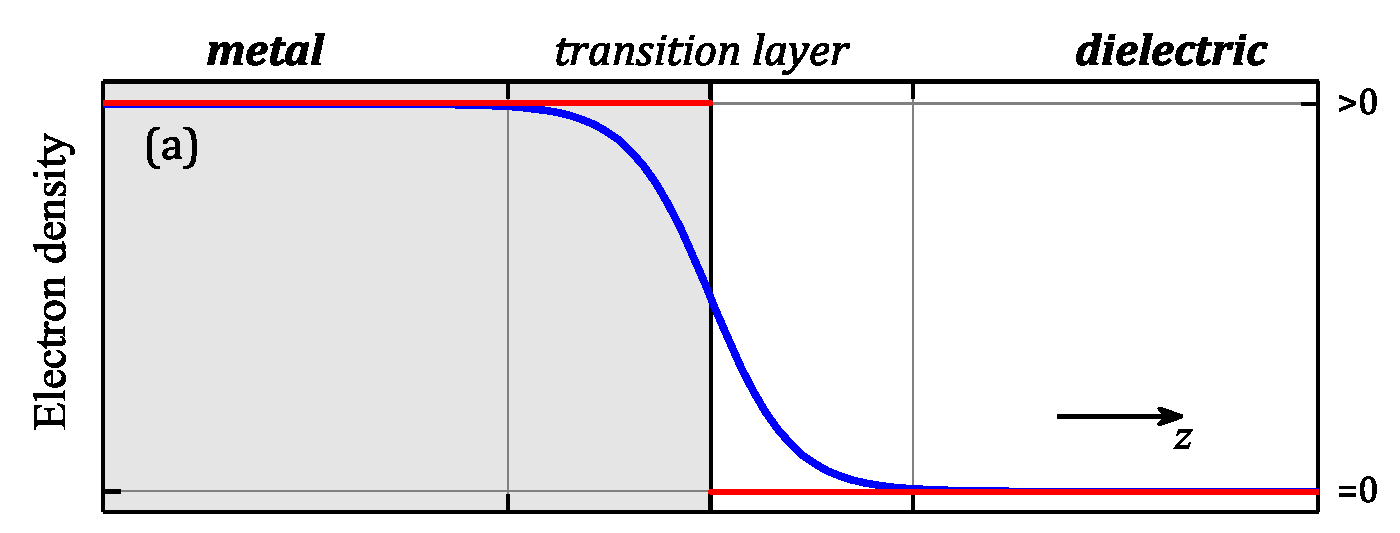
\includegraphics[width=\linewidth]{transitionA.eps}
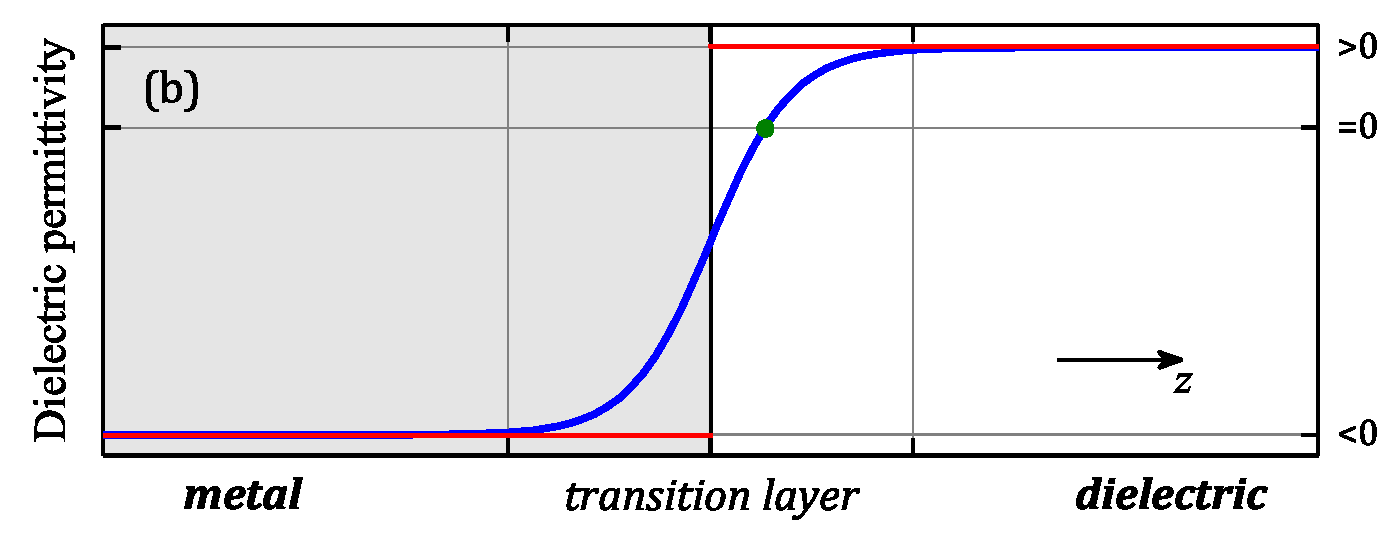
\includegraphics[width=\linewidth]{transitionB.eps}
\caption{Electron density (a) and dielectric permittivity (b) profiles in the vicinity of the metal-dielectric interface. The qualitative behavior for these two quantities is shown assuming the ideally sharp boundary (red lines) and the smooth transition of material properties (blue curves). At some critical point located in the dielectric close to the metal surface, the dielectric permittivity becomes zero (green dot).}
\label{fig:profilePlasmon}
\end{figure}

The~exact solution for the~electron density profile is known to feature the~so-called Friedel oscillations \cite{friedel}, but in this study, I will assume the~electron density to be monotonically decreasing away from metal (see \cref{fig:profilePlasmon}).
This simplification is justified by the~fact that the~qualitative behavior of the~SPP does not depend on the~particular choice of the~electron distribution within the~transition layer (see the~discussion in \cite{prigogine}).
As a result, the analysis presented below does not rely on a particular choice of the dielectric permittivity profile, as opposed to the studies \cite{akimov,gabitov1,gabitov2}, and, moreover, can be generalized to 2D or 3D geometries.

One may also wonder whether the use of macroscopic parameters to describe the ENZ layer is justified at all.
Indeed, the typical size of the transition layer varies from several angstrom to several nanometers \cite{akimov}, which is at least an order of magnitude larger than the characteristic inter-atomic distance in the bulk of the media.
This way the ENZ layer is populated by a sufficient number of spillout electrons, whose collective response to the electromagnetic field is then best described by the macroscopic dielectric permittivity.


%%%%%%%%%%%%%%%%%%%%%%%%%%%%%%%%%%%%%%%%%%%%%%%%%%%%%%%%%%%%%%%%%%%%
\section{Wave Equation for SPP Propagation}

Let us consider a~general case of a~system consisting of dielectric and metallic regions, which alternate along the~$z$-direction and are uniform and isotropic in $x$- and $y$-directions.
In this system, the~dielectric permittivity at any point can be written as $\epsilon = \epsilon(z)$, which may be either continuous or discontinuous function of the~coordinate $z$.

The~electromagnetic field in the~system is a~solution of the~Maxwell's equations:
%
\begin{align}
\nabla \times \mathbf{E} &= -\dfrac{1}{c} \dfrac{\partial \mathbf{H}}{\partial t}, \label{eq:maxwellE} \\
\nabla \times \mathbf{H} &= +\dfrac{1}{c} \dfrac{\partial \mathbf{D}}{\partial t}, \label{eq:maxwellH}
\end{align}
%
where the~electric displacement is $\mathbf{D} = \epsilon \mathbf{E}$, and the~uniform magnetic susceptibility of $\mu = 1$ is assumed.

It is well-known that any plasmonic mode supported by such structure must be a~$p$-polarized (transverse magnetic or TM) wave propagating along the~metal-dielectric interface.
Therefore, without any loss of generality, one may seek the~solutions for the~SPP mode in the~form of a~monochromatic running wave
%
\begin{equation}
\label{eq:runningH}
\mathbf{H} = H_y(z) e^{ikx - i\omega t}\hat{\mathbf{e}}_y,
\end{equation}
%
with the~magnetic field $\mathbf{H}$ being parallel to the~interface between media and perpendicular to the~direction of propagation.
Replacing thus the~time derivative $\partial/\partial t$ with $-i\omega$ and eliminating the~electric field from \cref{eq:maxwellE,eq:maxwellH}, one obtains the~following wave equation:
%
\begin{equation*}
\nabla\times \left( \dfrac{1}{\epsilon} \nabla\times\mathbf{H} \right) = \dfrac{\omega^2}{c^2} \mathbf{H},
\end{equation*}
%
which can be simplified and written down in terms of $H_y(z)$ as
%
\begin{equation}
\label{eq:waveeqPlasmon}
\dfrac{d}{dz}\left(\dfrac{1}{\epsilon(z)}\dfrac{dH_y}{dz}\right) + \left(\dfrac{\omega^2}{c^2}-\dfrac{k^2}{\epsilon(z)}\right)H_y(z) = 0.
\end{equation}
%
This is the~well-known equation for the~$p$-polarized electromagnetic waves propagating in a~nonuniform medium \cite{LLtom8}.
The~subscript "$y$" will be omitted everywhere below as the~magnetic field will be assumed to always point along the~$y$-axis.

\section{SPP Dispersion and Field Profiles: Ideal Case}

Before addressing the~SPP propagation problem along the~transition layer, I will briefly summarize the~main properties that are distinct to the~SPP propagating along the~sharp boundary.
As will be seen further, knowing the SPP magnetic field distribution and its dispersion in the case of ideal boundary allows one to analytically calculate the SPP dispersion corrections due to the presence of the transition layer.


\subsection{Single-Interface System}

In the~case of a~discontinuous dielectric function profile
\begin{equation}
\label{eq:idealeps1Plasmon}
\epsilon_0(z)~=~\left[
\begin{aligned}
&\epsilon_d, &z>0,\\
&\epsilon_m, &z<0,
\end{aligned}
\right.
\end{equation}
which describes an~ideal interface between metallic ($\epsilon_m<0$) and dielectric ($\epsilon_d>0$) semi-spaces, the~plasmonic solution of the~wave equation \cref{eq:waveeqPlasmon} is well-known \cite{zayats}:
\begin{equation}
\label{eq:idealeps1HfieldPlasmon}
H_0(z)~=~H_0 \times \left[
\begin{aligned}
&e^{-\kappa_d z}, &z>0,\\
&e^{+\kappa_m z}, &z<0,\\
\end{aligned}
\right.
\end{equation}
where $\kappa_{d,m} = \sqrt{k^2-\epsilon_{d,m}\omega^2/c^2}$, and the~SPP dispersion $\omega=\omega_0(k)$ is given by
\begin{equation}
\label{eq:idealeps1dispPlasmon_2}
\frac{\epsilon_m}{\epsilon_{d}}\frac{\kappa_{d}}{\kappa_m}+1~=~0
\end{equation}
or
\begin{equation}
\label{eq:idealeps1dispPlasmon}
k~=~\frac{\omega}{c}\sqrt{\frac{\epsilon_d\epsilon_m}{\epsilon_d+\epsilon_m}}.
\end{equation}

Note that in order to solve the~wave equation with the~discontinuous dielectric function, the~boundary conditions for both magnetic and longitudinal electric fields must hold, namely, the~functions $H_0(z)$ and $\epsilon_0^{-1}(z)\dfrac{dH_0}{dz}$ must be continuous.

From now on, the~quantities with the~subscript "$0$" will be describing the~SPP properties in cases with ideal boundaries.



\subsection{Double-Interface System}

In the~case of a~discontinuous dielectric function profile
\begin{equation}
\label{eq:idealeps2Plasmon}
\epsilon_0(z)~=~\left[
\begin{aligned}
&\epsilon_{d+}, &z>+s,\\
&\epsilon_m, &|z|<s, \\
&\epsilon_{d-}, &z<-s,
\end{aligned}
\right.
\end{equation}
which corresponds to a~metal film of thickness $2s$ clad between two different bulk dielectrics (with permittivities $\epsilon_{d+}$ and $\epsilon_{d-}$, respectively), the~SPP dispersion is implicitly given \cite{zayats} by the~following equation:
\begin{equation}
\label{eq:idealeps2dispPlasmon}
\left(\frac{\epsilon_m}{\epsilon_{d+}}\frac{\kappa_{d+}}{\kappa_m}+1\right)\left(\frac{\epsilon_m}{\epsilon_{d-}}\frac{\kappa_{d-}}{\kappa_m}+1\right)~=~\left(\frac{\epsilon_m}{\epsilon_{d+}}\frac{\kappa_{d+}}{\kappa_m}-1\right)\left(\frac{\epsilon_m}{\epsilon_{d-}}\frac{\kappa_{d-}}{\kappa_m}-1\right) e^{-4\kappa_m s}.
\end{equation}
Its solutions represent coupled modes, meaning that the~SPP on one interface is intertwined with that on the~other interface due to the~small thickness of the~film.
For a~sufficiently thick metal film, however, $s \rightarrow \infty$, the~dispersion relation \cref{eq:idealeps2dispPlasmon} naturally decouples into two:
\begin{equation}
\frac{\epsilon_m}{\epsilon_{d\pm}}\frac{\kappa_{d\pm}}{\kappa_m}+1~=~0,
\end{equation}
which separately describe plasmonic modes existing independently on each interface (see the~dispersion equation \cref{eq:idealeps1dispPlasmon_2})

As for the~SPP magnetic field, I write it down as follows:
\begin{equation}
\label{eq:idealeps2HfieldPlasmon}
H_0(z)~=~H_0 \times \left[
\begin{aligned}
&\CA e^{-\kappa_{d+} (z-s)}, &z>+s,\\
&\CB e^{+\kappa_m z} + \CC e^{-\kappa_m z}, &|z|<s,\\
&\CD e^{+\kappa_{d-} (z+s)}, &z<-s,\\
\end{aligned}
\right.
\end{equation}
where the~coefficients $\CA$, $\CB$, $\CC$ and $\CD$ are related through the~boundary conditions at the~interfaces $z=\pm s$.
The~continuity of $H_0(z)$ and $\epsilon_0^{-1}(z)\dfrac{dH_0}{dz}$ yields
\begin{align}
\CA~=~\CB e^{+\kappa_m s} + \CC e^{-\kappa_m s},& \qquad
-\frac{\kappa_{d+}}{\epsilon_{d+}}\CA~=~\frac{\kappa_m}{\epsilon_m}\left(\CB e^{+\kappa_m s} - \CC e^{-\kappa_m s}\right), \\
\CD~=~\CB e^{-\kappa_m s} + \CC e^{+\kappa_m s},& \qquad
+\frac{\kappa_{d-}}{\epsilon_{d-}}\CD~=~\frac{\kappa_m}{\epsilon_m}\left(\CB e^{-\kappa_m s} - \CC e^{+\kappa_m s}\right).
\end{align}
The~solvability of such homogeneous linear system is guaranteed when the~dispersion equation \cref{eq:idealeps2dispPlasmon} is satisfied, and thus one of the~coefficients can be assigned an~arbitrary value and the~rest will be expressed through it.

Besides $s \rightarrow \infty$, there is another special case where the~metal film is surrounded by the~same dielectric, $\epsilon_{d+},\epsilon_{d-}=\epsilon_{d}$.
As a result, the~plasmonic modes can be classified as either even (also called long-range) or odd (short-range) with respect to the~coordinate $z$ (see \cite{zayats} for additional details).



%%%%%%%%%%%%%%%%%%%%%%%%%%%%%%%%%%%%%%%%%%%%%%%%%%%%%%%%%%%%%%%%%%%%
\section{SPP Field Inside the Transition Layer}

Despite the~fact that the~wave equation \cref{eq:waveeqPlasmon} has analytical solutions for only a~few particular functions $\epsilon(z)$, it is possible to analyze the~asymptotic behavior of the~magnetic and electric fields within the~ENZ transition layer in the~general case.
Let us assume first that in the~vicinity of the~critical point $z_c$, where the~dielectric function vanishes, $\epsilon(z_c)=0$, the~latter can be expanded in series up to the~first nonzero term as follows:
\begin{equation}
\epsilon(z) \approx \epsilon'(z_c)(z-z_c).
\end{equation}


\begin{figure}[ptb]
\begin{center}
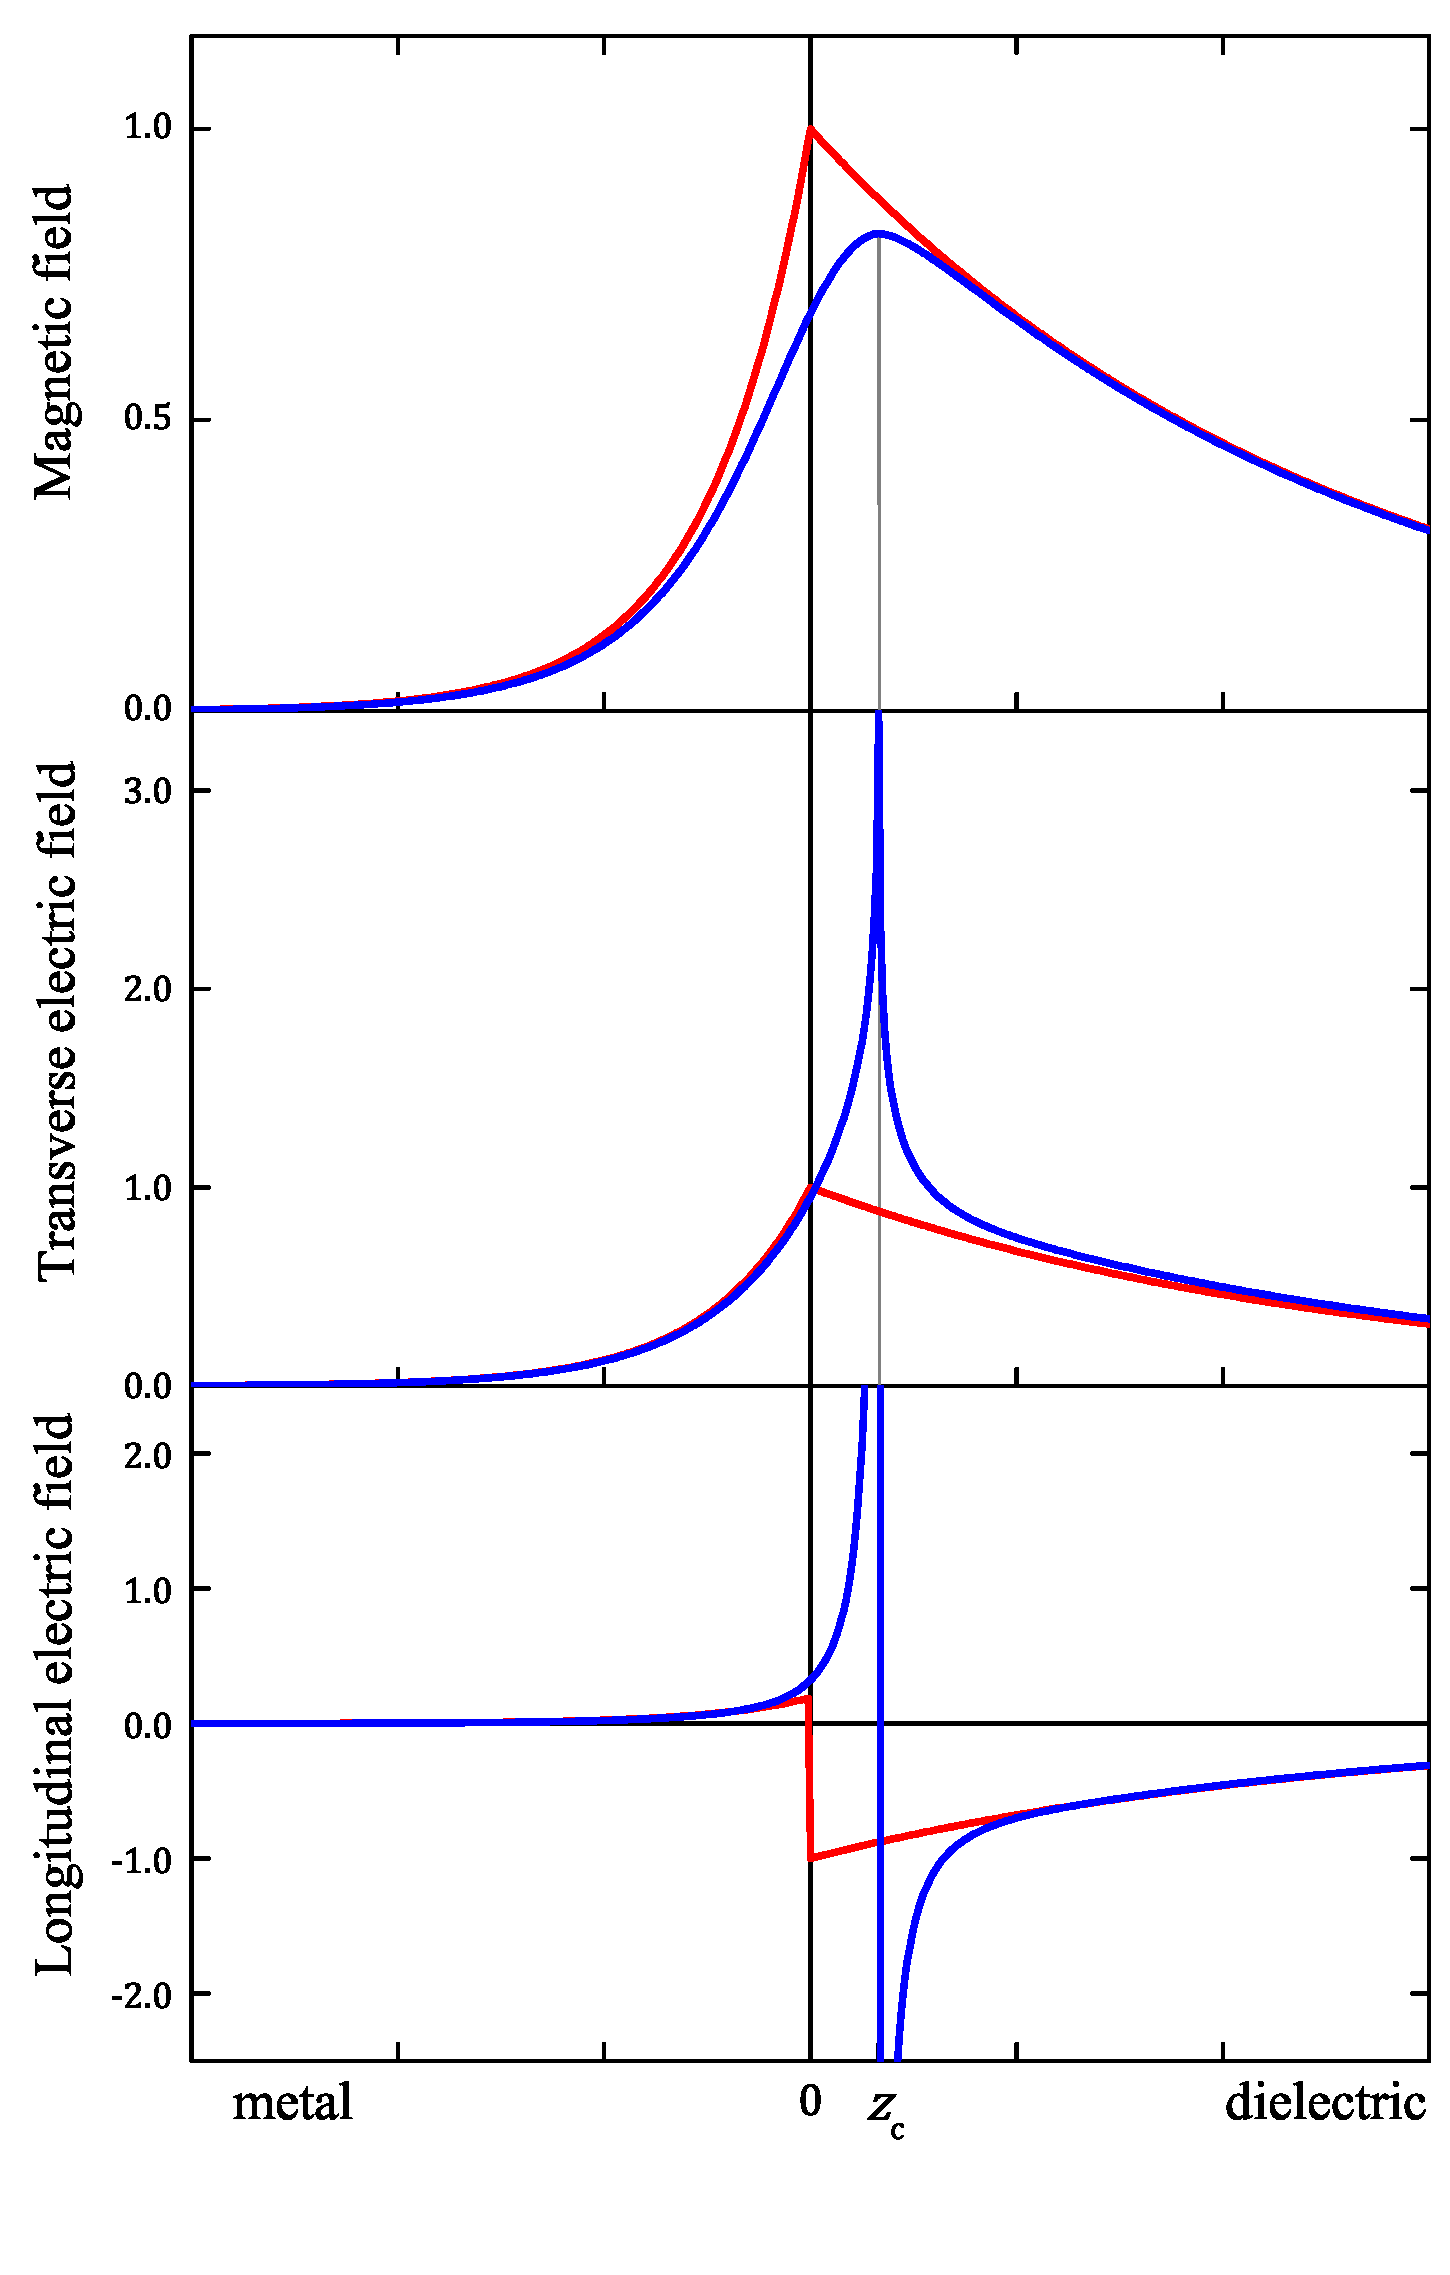
\includegraphics[width=0.75\linewidth]{EHfields.eps}
\caption{Asymptotic behavior of the SPP electromagnetic field (in a.u.) in the vicinity of the critical point $z_c$ (blue), in comparison with the case of no transition layer (red).}
\label{fig:EHfieldsPlasmon}
\end{center}
\end{figure}


Also, the~term $\omega^2/c^2$ can be neglected in comparison with $k^2/\epsilon(z)$ in the~wave equation.
With these assumptions, the~equation \cref{eq:waveeqPlasmon} can be written down as
\begin{equation}
\left(z-z_c\right)\dfrac{d}{dz}\left(\dfrac{1}{z-z_c}\dfrac{dH}{dz}\right)-k^2 H(z) = 0,
\end{equation}
and the~solution for $H(z)$, when $|z-z_c| \ll \delta$, is expressed via modified Bessel functions as
\begin{equation}
\label{eq:asymptFieldPlasmon}
H(\xi) = k\xi \left(C^{(1)} I_1\left(k\xi\right) + C^{(2)} K_1\left(k\xi\right)\right),
\end{equation}
where $\xi = z-z_c$.
The~parameter $\delta$ characterizes the~width of the~transition layer.
From \cref{eq:asymptFieldPlasmon} the~electric and magnetic fields asymptotically behave as
\begin{align}
&H(\xi) \sim 1+\dfrac12 k^2 \xi^2 \ln k\xi,\\
&E_x(\xi) \sim \dfrac{1}{\epsilon(\xi)}\dfrac{\partial H}{\partial \xi} \sim \ln k\xi,\\
&E_z(\xi) \sim \dfrac{H(\xi)}{\epsilon(\xi)} \sim \dfrac{1}{\xi}.
\end{align}
The~analysis shows that both components of the~electric field tend to infinity when $z \rightarrow z_c$ (see \cref{fig:EHfieldsPlasmon}).
Of course, such scenario is unrealistic, since there always are some inevitable losses within the~real materials and one cannot have a~pure real dielectric function, therefore the~growth of the~electric field is actually capped at a~level determined by the~imaginary part of $\epsilon(z_c)$ (see, e.g., \cite{ginzburg}).

Nevertheless, the~described electric field enhancement plays a defining role in optoelectronic devices.
In particular, the processes of spontaneous photon emission, according to the Purcell effect, occur much more often when the emitter is placed in the strong electromagnetic field \cite{schuller}.

%%%%%%%%%%%%%%%%%%%%%%%%%%%%%%%%%%%%%%%%%%%%%%%%%%%%%%%%%%%%%%%%%%%%
\section{Perturbation Theory}

Since the~thickness $\delta$ of the~ENZ transition layer is typically of the~order of several angstroms, this small parameter suggests that a~perturbation theory can be developed to calculate the~corrections to the~plasmonic spectrum.
From now on, the~problem of the~SPP propagation featuring ideal metal-dielectric interfaces will be considered an~unperturbed problem, and the~presence of the~ENZ layers will be treated as a~small perturbation.
It is easy to see, however, that a~continuous and smooth dielectric function $\epsilon(z)$ can never be represented as a~sum of the~unperturbed step-like function $\epsilon_0(z)$ and the~small correction proportional to $\delta$, which means the~wave equation \cref{eq:waveeqPlasmon} in its current form does not allow for the~perturbative approach.

\subsection{Integral Eigenvalue Problem}

With this, the~Fourier transformations of the~magnetic field of the~SPP and the~dielectric function are introduced in the~form of
\begin{equation}
\label{eq:fourierH}
H(z)~=~\int\limits_{-\infty}^{+\infty}h(p)e^{ipz}dp, \quad \textrm{where} \quad
h(p)~=~\frac{1}{2\pi}\int\limits_{-\infty}^{+\infty}H(z)e^{-ipz}dz,
\end{equation}
and
\begin{equation}
\label{eq:fourierEPS}
\frac{1}{\epsilon(z)}~=~\int\limits_{-\infty}^{+\infty}\eta(p)e^{ipz}dp, \quad \textrm{where} \quad
\eta(p)~=~\frac{1}{2\pi}\int\limits_{-\infty}^{+\infty}\frac{e^{-ipz}}{\epsilon(z)}dz.
\end{equation}
After applying the~Fourier transform to the~wave equation \cref{eq:waveeqPlasmon} as well, it takes the~following integral form:
\begin{equation}
\label{eq:inteqPlasmon}
\frac{\omega^2}{c^2}h\left(p\right)~=~\int\limits_{-\infty}^{+\infty}\left(k^2+pp'\right)\eta (p-p') h(p') dp'.
\end{equation}

Equation \cref{eq:inteqPlasmon} can be regarded as an~integral eigenvalue problem for the~plasmonic spectrum $\omega = \omega(k)$, which is valid for the~SPP on both ideal interface and interface with the~ENZ transition.
If the~integral kernel $K(p,p') = \left(k^2+pp'\right)\eta (p-p')$ satisfies the~condition $K(p,p')=K^{*}(p',p)$, which requires $\eta(p) = \eta^{*}(-p)$, the~problem is then Hermitian, and its solutions are true SPP modes with real eigenfrequencies $\omega$.

For the~unperturbed problem this is indeed the~case, because the~dielectric function $\epsilon_0(z)$ is pure real, and 
\begin{equation}
\eta_0(p)~=~\int\limits_{-\infty}^{+\infty}\frac{e^{-ipz}}{\epsilon_0(z)}dz
\end{equation}
is clearly equal to its Hermitian conjugate.

In the~presence of the~ENZ transition, the~function $1/\epsilon(z)$, while being still pure real, features a~singularity, so that in the~expression 
\begin{equation}
\label{eq:etaPlasmon}
\eta(p)~=~\dfrac{1}{2\pi} \int\limits_{-\infty}^{+\infty} \frac{e^{-ipz}}{\epsilon(z)}dz
\end{equation}
the~integration path must be curved to avoid this pole (see \cref{fig:polePlasmon}).
Therefore, the~Fourier transform of the~inverse dielectric function \cref{eq:etaPlasmon} can be rewritten as
\begin{equation}
\eta(p)~=~\dfrac{1}{2\pi} \fint\limits_{-\infty}^{+\infty} \frac{e^{-ipz}}{\epsilon(z)}dz - \frac{i}{2}\,\underset{z=z_0}{\mathrm{res}}\frac{e^{-ipz}}{\epsilon(z)},
\end{equation}
where the~integral is understood as its Cauchy principal value.
The~second term that appears due to the~singularity clearly breaks the~hermiticity of the~kernel in \cref{eq:inteqPlasmon}, and the~non-Hermitian eigenvalue problem thus results in complex eigenvalues $\omega = \omega(k) = \omega'(k) - i\omega''(k)$.

The~imaginary part of the~eigenvalue $\omega$ means that the~SPP would inevitably lose energy even if the~metal is lossless.
The~very existence of the~critical point in the~ENZ transition layer results in the~delocalization of the~plasmon energy, which therefore gradually radiates away from the~interface and depletes the~plasmon.
This novel mechanism of the~SPP decay is in some sense similar to the~Landau damping mechanism \cite{LLtom8}, since neither is due to the~electron collisions in metal, and the~difference is that the~SPP does not channel energy to the~resonant electrons, but rather couples to the~bulk plasmons in the~transition layer \cite{akimov}.

This radiative plasmonic decay was earlier reported to exist for some specially tailored dielectric permittivity profiles in a~two-layered system (see, e.g., \cite{akimov}), however, the~goal of my work is to develop a~theoretical approach that is capable of calculating the~SPP dispersion for \textit{any} function $\epsilon(z)$ and, specifically, for systems with \textit{any} number of layers, and that can also be generalized for 2D or 3D problems.

\subsection{Linear Perturbation}

Let us now seek the~solution of the~integral eigenvalue problem \cref{eq:inteqPlasmon} in the~linear order of the~perturbation theory in the~form of
\begin{equation}
\label{eq:deltaomegaPlasmon}
\omega~=~\omega(k)~=~\omega_0(k)+\Delta \omega(k),
\end{equation}
\begin{equation}
\label{eq:deltaetaPlasmon}
\eta(p)~=~\eta_0(p)+\Delta\eta(p),
\end{equation}
\begin{equation}
\label{eq:deltahPlasmon}
h(p)~=~h_0(p)+\Delta h(p),
\end{equation}
where $\omega_0(k)$, $\eta_0(p)$ and $h_0(p)$ describe the~spectrum, the~dielectric permittivity and the~magnetic field of the~SPP in the~unperturbed case, and the~corrections $\Delta \omega(k)$, $\Delta \eta(p)$ and $\Delta h(p)$ are proportional to the~small parameter $\delta$.

Substituting \cref{eq:deltaomegaPlasmon}-\cref{eq:deltahPlasmon} into \cref{eq:inteqPlasmon} and discarding quadratic over $\delta$ terms, one arrives at the~Fredholm integral equation of the~second kind for $\Delta h(p)$:
\begin{equation}
\label{eq:fredholmPlasmon}
\frac{\omega_0^2}{c^2}\Delta h\left(p\right)-\int\limits_{-\infty}^{+\infty}\left(k^2+pp'\right)\eta_0 (p-p') \Delta h(p') dp'~=~-\frac{2\omega_0\Delta \omega}{c^2}h_0\left(p\right)+F(p),
\end{equation}
where the~last term in the~right-hand side is
\begin{equation}
\label{eq:FpPlasmon}
F(p)~=~\int\limits_{-\infty}^{+\infty}\left(k^2+pp'\right)\Delta\eta (p-p') h_0(p') dp'.
\end{equation}
According to one of the~Fredholm's theorems \cite{fredholm}, the~solution of the~inhomogeneous Fredholm equation \cref{eq:fredholmPlasmon} exists if and only if the~inhomogeneous term is orthogonal to the~solution of the~adjoint homogeneous equation, i.e., if
\begin{equation}
\label{eq:fredholmtheoremPlasmon}
\int\limits_{-\infty}^{+\infty} \left(-\frac{2\omega_0\Delta \omega}{c^2}h_0\left(p\right)+F(p)\right) h_0^{*}(p) dp~=~0,
\end{equation}
where the~solution of the~homogeneous equation is nothing else but the~unperturbed magnetic field $h_0(p)$.
This orthogonality condition immediately gives the~spectrum correction $\Delta \omega$:
\begin{equation}
\label{eq:correctionPlasmon}
\dfrac{\Delta\omega}{\omega_0}~=~\frac{c^2}{2\omega_0^2}\frac{\int\limits_{-\infty}^{+\infty}F(p)h_0^{*}(p)dp}{\int\limits_{-\infty}^{+\infty}h_0(p)h_0^{*}(p)dp}.
\end{equation}
The~denominator can be further simplified using the~relation \cref{eq:fourierH}:
\begin{equation}
\int\limits_{-\infty}^{+\infty}h_0(p)h_0^{*}(p)dp~=~\frac{1}{2\pi}\int\limits_{-\infty}^{+\infty}H_0(z)H_0^{*}(z)dz~=~\frac{1}{2\pi}\int\limits_{-\infty}^{+\infty}\left|H_0(z)\right|^2 dz,
\end{equation}
which yields
\begin{equation}
\label{eq:correctionPlasmon2}
\dfrac{\Delta\omega}{\omega_0}~=~\frac{\pi c^2}{\omega_0^2}\frac{\int\limits_{-\infty}^{+\infty}F(p)h_0^{*}(p)dp}{\int\limits_{-\infty}^{+\infty}\left|H_0(z)\right|^2 dz}.
\end{equation}
In order to evaluate the~numerator, I rewrite the~expression for $F(p)$ as
\begin{equation}
\begin{aligned}
F(p)~&=~\int\limits_{-\infty}^{+\infty} dp'(k^2+pp')\Delta\eta(p-p')h_0(p') = \\
&=~\frac{1}{2\pi}\int\limits_{-\infty}^{+\infty}dp' (k^2+pp')h_0(p')\left(\int\limits_{-\infty}^{+\infty}dz e^{-i(p-p')z}\left(\frac{1}{\epsilon(z)}-\frac{1}{\epsilon_0(z)}\right)\right) = \\
&=~\frac{1}{2\pi}\int\limits_{-\infty}^{+\infty}dz \left(\frac{1}{\epsilon(z)}-\frac{1}{\epsilon_0(z)}\right)e^{-ipz} \left(\int\limits_{-\infty}^{+\infty}dp' (k^2+pp')h_0(p') e^{ip'z}\right) = \\,
&=~\frac{1}{2\pi}\int\limits_{-\infty}^{+\infty}dz \left(\frac{1}{\epsilon(z)}-\frac{1}{\epsilon_0(z)}\right)e^{-ipz} \CF(z,p),
\end{aligned}
\end{equation}
where the~order of integrations was changed to allow for the~calculation of the~inner integral over $p$. Using the~identities for the~Dirac delta function \cref{eq:app_diracdelta1}-\cref{eq:app_diracdelta4}, this inner integral, $\CF(z,p)$, is significantly simplified:
\begin{align}
\CF(z,p)~&=~\int\limits_{-\infty}^{+\infty}dp' (k^2+pp')h_0(p') e^{ip'z}~= \\
&=~\int\limits_{-\infty}^{+\infty}dp' (k^2+pp')e^{ip'z}\left(\frac{1}{2\pi}\int\limits_{-\infty}^{+\infty}dz'H_0(z')e^{-ip'z'}\right)~=\notag\\
&=~\frac{1}{2\pi} \int\limits_{-\infty}^{+\infty} dz' H_0(z')\left(\int\limits_{-\infty}^{+\infty} dp' (k^2+pp')e^{ip'(z-z')}\right)~=\notag\\
&=~\int\limits_{-\infty}^{+\infty} dz' H_0(z')\Big(k^2\delta(z-z')+i p \delta'(z-z')\Big)~=~k^2 H_0(z)-ip H_0'(z),\notag
\end{align}
Consequently, the~numerator of \cref{eq:correctionPlasmon2} is reduced to
\begin{equation}
\begin{aligned}
\int\limits_{-\infty}^{+\infty} F(p)h_0^*(p)dp~&=~\frac{1}{2\pi}\int\limits_{-\infty}^{+\infty} dp\,h_0^*(p) \left( \int\limits_{-\infty}^{+\infty}dz \left(\frac{1}{\epsilon(z)}-\frac{1}{\epsilon_0(z)}\right)e^{-ipz} \CF(z,p)\right)~= \\
&=~\frac{1}{2\pi} \int\limits_{-\infty}^{+\infty}dz \left(\frac{1}{\epsilon(z)}-\frac{1}{\epsilon_0(z)}\right) \left( \int\limits_{-\infty}^{+\infty} dp\,\CF(z,p) h_0^*(p) e^{-ipz}\right)~= \\
&=~\frac{1}{2\pi} \int\limits_{-\infty}^{+\infty}dz \left(\frac{1}{\epsilon(z)}-\frac{1}{\epsilon_0(z)}\right) G(z),
\end{aligned}
\end{equation}
with the~function $G(z)$ being
\begin{align}
&G(z)~=~\int\limits_{-\infty}^{+\infty} dp\,\CF(z,p) h_0^*(p) e^{-ipz}~=\\
&=~\int\limits_{-\infty}^{+\infty}dp \Big(k^2 H_0(z)-ip H_0'(z)\Big)e^{-ipz}\left(\frac{1}{2\pi}\int\limits_{-\infty}^{+\infty} dz'H_0^{*}(z')e^{ipz'}\right)~=\notag\\
&=~\frac{1}{2\pi} \int\limits_{-\infty}^{+\infty}dz' H_0^{*}(z')\left(k^2H_0(z)\int\limits_{-\infty}^{+\infty}dp\,e^{ip(z-z')} - iH_0'(z) \int\limits_{-\infty}^{+\infty}dp\,pe^{ip(z-z')}\right)~=\notag\\
&=~\int\limits_{-\infty}^{+\infty}dz' H_0^{*}(z')\Bigg(k^2H_0(z)\delta(z-z')-H_0'(z)\delta'(z-z')\Bigg)~=~k^2|H_0(z)|^2+|H_0'(z)|^2,\notag
\end{align}
Ultimately, the~eigenfrequency shift $\Delta\omega$ takes the~form which explicitly depends on the~magnetic field $H_0(z)$ and the~dielectric permittivities $\epsilon_0(z)$ and $\epsilon(z)$ only:
\begin{equation}
\label{eq:correctionPlasmon3}
\frac{\Delta\omega}{\omega_0}~=~\frac{c^2}{2\omega_0^2}\frac{\int\limits_{-\infty}^{+\infty}\left(\frac{1}{\epsilon(z)}-\frac{1}{\epsilon_0(z)}\right) \Big(k^2|H_0(z)|^2+|H_0'(z)|^2\Big)dz}{\int\limits_{-\infty}^{+\infty} |H_0(z)|^2 dz}.
\end{equation}


\subsection{Analysis of the Eigenfrequency Shift}

Every term in the~right-hand side of \eqref{eq:correctionPlasmon3} is pure real, yet the~integration in the~numerator results in a~complex value since one has to carefully handle the~singularities in $\frac{1}{\epsilon(z)}$, which are located at the~points where $\epsilon(z)=0$.
The~integration path must therefore be bent into the~complex $z$ plane in order to avoid the~poles $z_\sigma$, $\sigma=1,2,3,...$, distributed along the~real axis.
Curving the~integration path in the~vicinity of the~poles adds a~small imaginary part to the~function $\epsilon(z)$, and in order to perform the~integration I make use of the~following well-known identity from the~complex analysis:
\begin{equation}
\frac{1}{z-z_\sigma\pm i 0^{+}}~=~P\frac{1}{z-z_\sigma}\mp i\pi\delta(z-z_\sigma),
\end{equation}
which is a~shorthand notation for
\begin{equation}
\label{eq:plemel}
\lim_{\alpha\to 0^{+}} \int\limits_{-\infty}^{+\infty}\frac{f(z)}{z-z_\sigma\pm i\alpha}dz~=~\fint\limits_{-\infty}^{+\infty}\frac{f(z)}{z-z_\sigma}dz \mp i\pi f(z_\sigma)
\end{equation}
that is valid for an~analytic function $f(z)$.
The~integral expression in the~right is understood as its Cauchy principal value.
The~choice of the~sign of the~imaginary part for each $z_\sigma$ is determined by whether the~pole must be circumflexed in the~upper or lower semispace of the~complex plane $z$ (see \cref{fig:polePlasmon}).

%
% FIGURE #
%
\begin{figure}[ptb]
\begin{center}
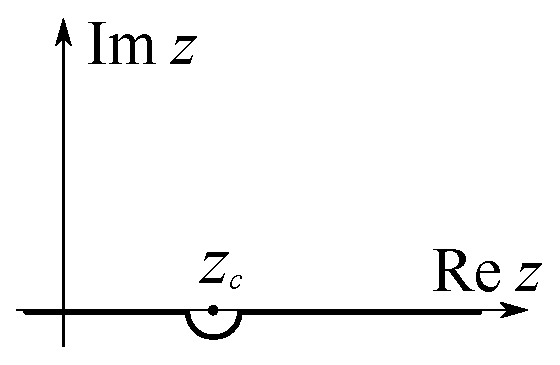
\includegraphics[width=8cm]{pole.eps}
\caption{Integration path is curved into the~lower semispace to avoid the~pole $z_c$ on the~real axis.}
\label{fig:polePlasmon}
\end{center}
\end{figure}


In general, the~pole is integrated around in a~way that is consistent with the~causality, i.e., its contribution to $\Delta\omega$ must have negative imaginary part to guarantee that the~SPP amplitude would not be exponentially increasing with time.

With that, one can separate the~real part of $\Delta\omega$:
\begin{equation}
\label{eq:correctionPlasmonRe}
\frac{\Delta\omega'}{\omega_0}~=~\frac{\re\Delta\omega}{\omega_0}~=~\frac{c^2}{2\omega_0^2}\frac{\fint\limits_{-\infty}^{+\infty}\left(\frac{1}{\epsilon(z)}-\frac{1}{\epsilon_0(z)}\right) \Big(k^2|H_0(z)|^2+|H_0'(z)|^2\Big)dz}{\int\limits_{-\infty}^{+\infty} |H_0(z)|^2 dz},
\end{equation}
from its imaginary part:
\begin{equation}
\label{eq:correctionPlasmonIm}
\frac{\Delta\omega''}{\omega_0}~=~-\frac{\im\Delta\omega}{\omega_0}~=~\frac{\pi c^2}{2\omega_0^2}\frac{\underset{\sigma}{\sum} |\epsilon'(z_\sigma)|^{-1} \Big(k^2|H_0(z_\sigma)|^2+|H_0'(z_\sigma)|^2\Big)}{\int\limits_{-\infty}^{+\infty} |H_0(z)|^2 dz}.
\end{equation}
Here I assumed the~linear behavior of the~dielectric function $\epsilon(z)$ in the~vicinity of each critical point: $\epsilon(z)\approx\epsilon'(z_\sigma)\left(z-z_\sigma\right)$, so that the~function $f(z)$ from the~identity \eqref{eq:plemel} corresponds to $\epsilon'(z)^{-1}\left(k^2|H_0(z)|^2+|H_0'(z)|^2\right)$.
The~integration path bends into the~lower semispace of the~complex plane $z$ for the~poles where $\epsilon'(z_\sigma)>0$, and into the~upper semispace otherwise. 

In addition, I emphasize that the~pure real nature of the~functions $\epsilon(z)$ and $\epsilon_0(z)$ was only used to simplify the~numerator in \eqref{eq:correctionPlasmon3}, which means the~expression for the~spectrum correction \eqref{eq:correctionPlasmon3} is valid even if the~dielectric functions are initially assumed to be complex, i.e., if they originally included the~dissipation losses as their imaginary parts.

Also, since I did not assume any particular dependence of the dielectric function on the coordinate $z$, except its linear behavior close to the critical points, the result of \cref{eq:correctionPlasmonRe} can formally take values of any sign.
This raises the question of how to limit our consideration to only those choices for $\epsilon(z)$ that are realistic and physically meaningful.
One way to do that is to obtain the plasmonic spectrum experimentally and extract the information about the sign of $\Delta\omega'$.
Knowing the sign of the left hand side of \cref{eq:correctionPlasmonRe}, one will know the sign of the integral $\fint\limits_{-\infty}^{+\infty}\left(\frac{1}{\epsilon(z)}-\frac{1}{\epsilon_0(z)}\right) \Big(k^2|H_0(z)|^2+|H_0'(z)|^2\Big)dz$ as well and thus can make an educated guess about the behavior of the dielectric function $\epsilon(z)$.

Finally, I note that in some situations it is more convenient to describe exactly the same behavior of the SPP by the pure real frequency $\omega$ and the complex wavevector $k=k(\omega)=k'(\omega)+ik''(\omega)$.
With respect to the perturbation theory, the connection between the two approaches can be established for small corrections $\Delta\omega$ and $\Delta k$ in the form of
\begin{equation}
\label{eq:omegatokPlasmon}
\Delta\omega'=-\left|\frac{d\omega}{dk}\right|\Delta k', \qquad
\Delta\omega''=\left|\frac{d\omega}{dk}\right|\Delta k'',
\end{equation}
via the group velocity $d\omega/dk$ of the unperturbed SPP mode.
Alternatively, one can explicitly use a similar perturbative approach to calculate $\Delta k$ from \cref{eq:inteqPlasmon}.

\section{SPP Dispersion}

\begin{figure}[ptb]
\subfloat{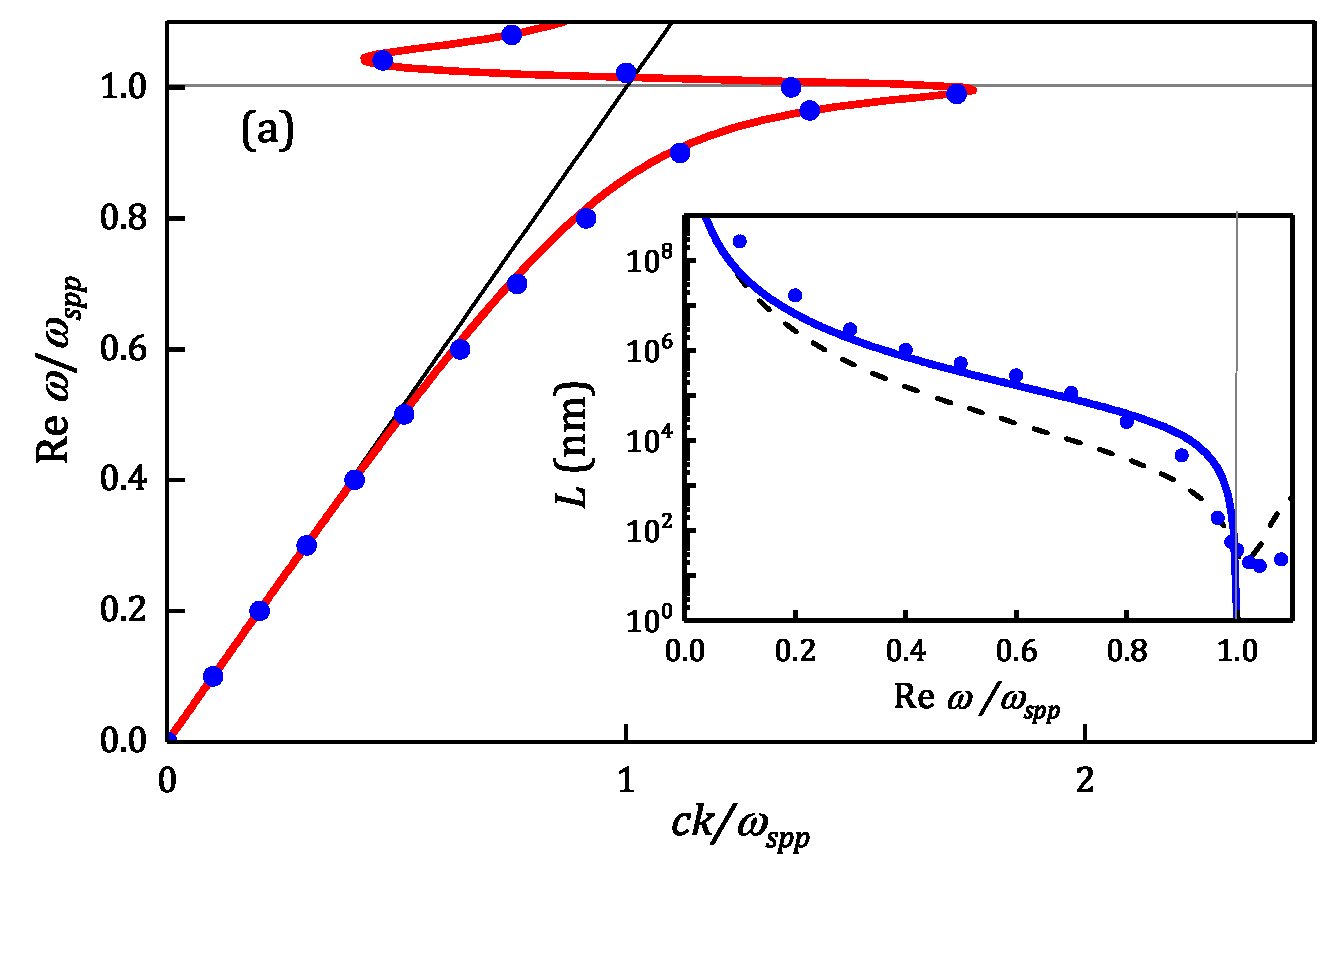
\includegraphics[clip,width=0.75\linewidth]{disp_bulk_2.eps}}

\subfloat{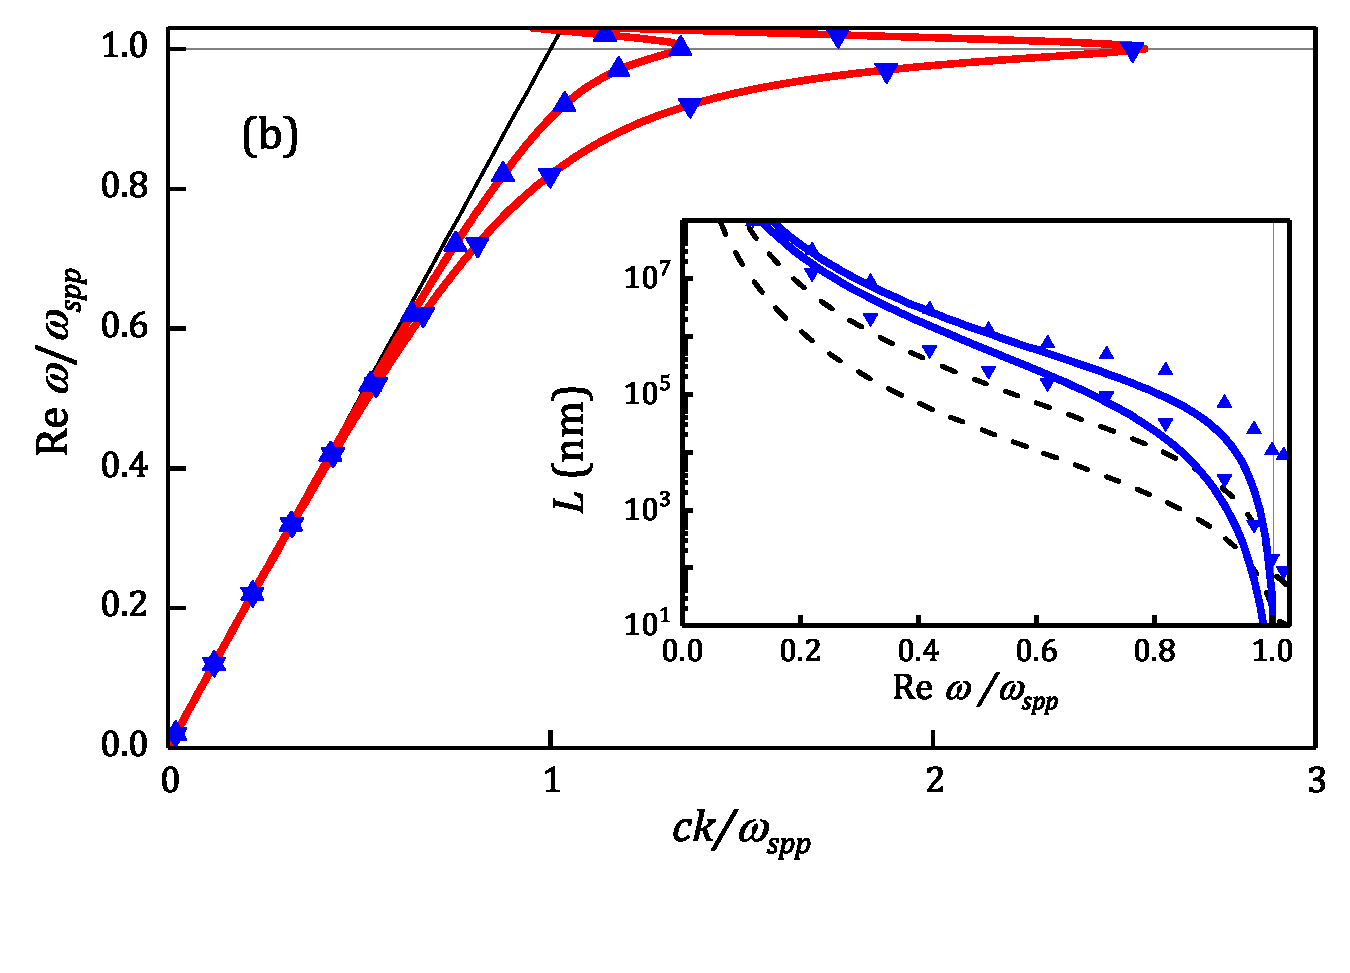
\includegraphics[clip,width=0.75\linewidth]{disp_thin_2.eps}}
\caption{SPP dispersion for the bulk (a) and 50nm-thick (b) silver slabs in air. The red curves and blue data points show the dispersion for the cases of ideal and realistic (with $\delta=0.02$nm) interfaces, respectively. The insets compare theoretical (blue lines) and numerical (blue data points) results for the SPP collisionless damping rates, expressed in terms of propagation length. The rate of Joule losses is shown with dashed black lines.}
\label{fig:dispersionPlasmon}
\end{figure}

Validating the theoretical predictions requires performing a number of numerical simulations.
In every simulation, I model the continuous metal-dielectric transitions with the dielectric function
\begin{equation}
\label{eq:epsilonContinuous}
\epsilon(z)~=~\epsilon_d + \frac{\epsilon_m-\epsilon_d}{1+e^{z/\delta}},
\end{equation}
where the parameter $\delta$ defines the transition layer thickness (see \cref{fig:profilePlasmon}).

Here I compare the predictions of the perturbation theory with the SPP dispersion corrections calculated numerically.
In order to do that, I numerically find the eigenvalues $\omega$ of the wave equation \cref{eq:waveeqPlasmon} for given wavevector $k$ and permittivity $\epsilon(z)$ as follows.
The eigenvalue $\omega$ is initially set equal to that of the unperturbed spectrum: $\omega=\omega_0(k)$.
The wave equation is then independently solved in the two regions, $z>0$ and $z<0$, with the specified asymptotic behavior imposed towards both infinities according to $|H(z)| \underset{z\rightarrow \pm\infty}{\longrightarrow} 0$.
The two solutions are renormalized to satisfy the magnetic field continuity $H(0^{+})=H(0^{-})$, and the value of the goal function $|E_x(0^{+})-E_x(0^{-})|$ is computed.
If the obtained value is lower than some set threshold, the longitudinal electric field $E_x(z)$ is considered to be continuous as well and the eigenvalue $\omega$ is thus found; otherwise, the optimization procedure is run to minimize the goal function, sweeping over the region of complex $\omega$.

I calculated the SPP dispersion for the cases of bulk and 50nm-thick silver slabs surrounded by air (see \cref{fig:dispersionPlasmon}).
For the dielectric permittivity of silver, I used the experimental data from \cite{johnson} that was fit by the generalized Lorentz-Drude model as described in \cite{rakic} (see Appendix~\ref{appSilver} for details).
Here $\delta=0.02$ nm, so that the thickness of the ENZ layer is on the order of 1 \AA.

In both cases, there were no drastic changes to the real part of the SPP dispersion due to including the ENZ transition layer into consideration, as seen from the main panels in \cref{fig:dispersionPlasmon}.
Instead, of particular interest are the results shown in the insets, where the imaginary part of $\omega$ is plotted in terms of the SPP propagation length.
The propagation length $L$ measures the distance over which the plasmon energy decreases by a factor of $e$ and can be expressed in terms of $\omega''$ as $L=(2 \omega'')^{-1} |d\omega/dk|$.

For the bulk sample, there is a good agreement between the theoretical and numerical estimations of the SPP decay rate that is only due to the SPP radiation through the critical point where $\epsilon(z)=0$.
When approaching the plasmon resonance frequency, the perturbation theory predicts much faster decay than the numerical calculation.
This happens because at high frequencies, one may no longer assume the perturbation to be small (the condition $k\delta \ll 1$ is not valid anymore), and the perturbation theory is no longer applicable.

For the thin film sample, there is also a good agreement for the high-frequency SPP mode, while the solution for the low-frequency SPP mode either under- or overestimates the numerically simulated propagation length, which is probably due to the perturbation theory exceeding its validity region.

For the reference, both insets also display the SPP propagation length that is only due to the Joule losses in metal in the Drude model.
This dissipative decay rate grows with frequency considerably slower than the decay rate due to the SPP radiative losses, and above the certain frequency the radiative decay becomes the dominant channel for energy dissipation.



\section{Excitation of SPP in the Transition Layer}

\subsection{Experimental Motivation}

\begin{figure}[ptb]
\begin{center}
\subfloat{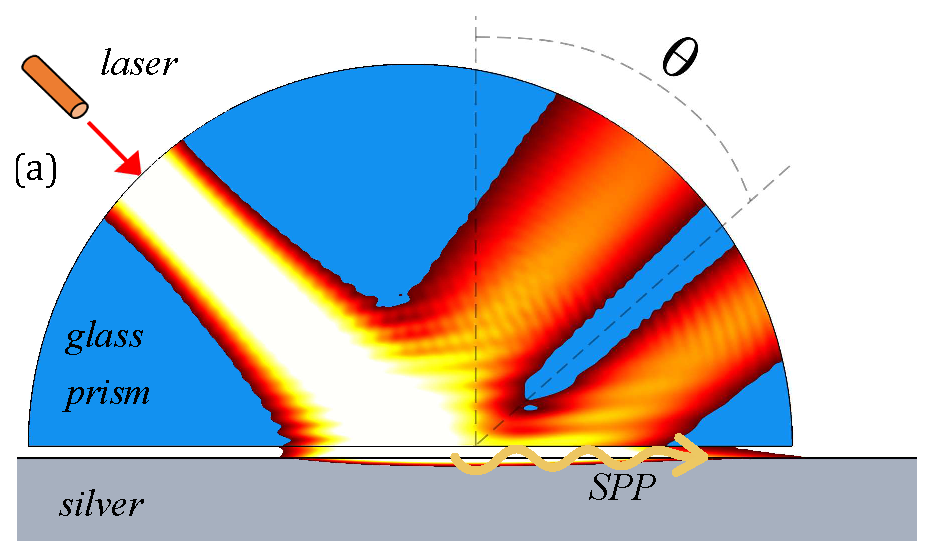
\includegraphics[clip,width=0.8\linewidth]{otto2.eps}}\\[1.0cm]
\subfloat{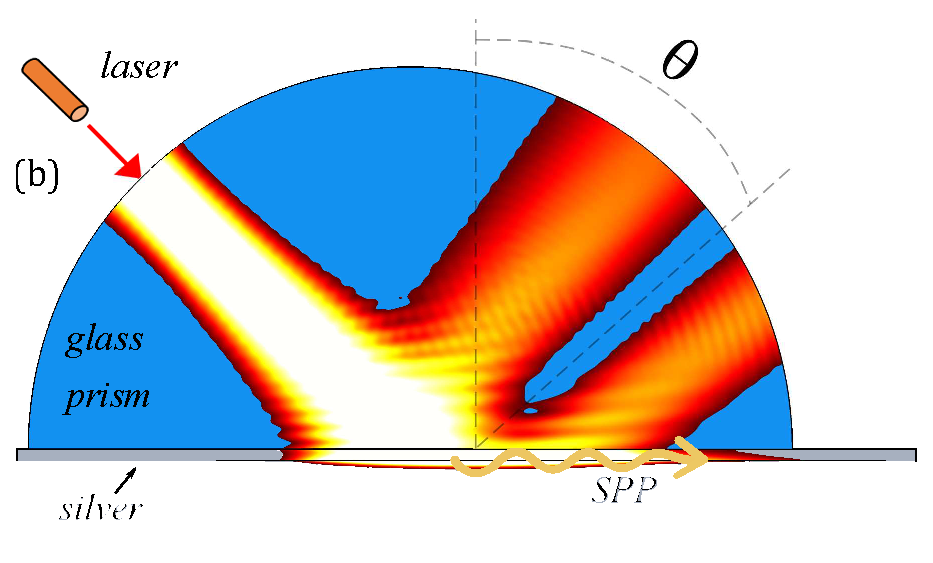
\includegraphics[clip,width=0.8\linewidth]{kret2.eps}}
\caption{Excitation of the SPP (a) on the silver slab in Otto configuration and (b) on the thin film in Kretschmann configuration \cite{raether}.}
\label{fig:ottosetupPlasmon}
\end{center}
\end{figure}

The two other simulations that were performed using the finite-element method modeled the excitation of the SPP by light.
In experiment such scenario is typically realized in either Otto or Kretschmann configuration \cite{raether}, where a laser beam propagates through a glass prism and is incident at an angle on a plasmonic sample.
The material of the prism must be more optically dense than the dielectric of the sample, which is a necessary condition that allows matching between the SPP wavevector and the parallel to the sample component of the wavevector of the laser.
In the absence of the prism the SPP excitation would never occur as the SPP wavevector $k_{SPP} > \omega/c$ would always be larger than the wavevector of light $k = \omega/c$.
The latter expresses the fact that SPPs propagate with the phase speed that is lower than the speed of light in corresponding dielectric medium.

\cref{fig:ottosetupPlasmon}(a) shows the excitation of SPP in the Otto configuration, which differs from the Kretschmann configuration on \cref{fig:ottosetupPlasmon}(b) only in the position of the prism.
Namely, in the Kretschmann configuration the prism sits on top of the metallic part of the plasmonic sample and the SPP is excited on the interface inside the sample, whereas in the Otto configuration the prism is separated from the sample by the air (or other dielectric) gap which leads to the SPP excitation along the interface between the air and the sample.
In the latter case the SPP may also be excited on the other interface of metal, provided the sample is relatively thin.
If it were thick, though, no excitation would reach that other interface due to the exponential weakening of the electromagnetic field as it propagates across the metallic layer.

Now, since one must also incorporate into setup the ability to control the width of the transition layer on the metal-dielectric interface by applying external DC field, the real sample would actually be a multi-layered structure.
Besides the possible dielectric substrate and index-matching layers, there have to be two outer layers serving as electrodes.
Such layers must be transparent for light, but still be able to conduct electricity.
Even though it is possible to find material that satisfies both these requirements (indium tin oxide, or ITO), one would need to carefully select the laser wavelength for the experiment in order to minimize losses in the auxiliary layers without getting too far from the SPP resonance.

It is for certain, however, that for the experiment with the bulk (thick) metallic sample only the Otto configuration is viable.
On the contrary, exciting SPPs on a thin metallic film benefits from the Kretschmann configuration as it becomes possible to negate the unavoidable issues with the uneven contact between the prism and the sample due to the surface roughness, e.g., by submerging the sample in the index matching liquid.


\subsection{Models for FEM Numerical Simulation}

For the purpose of comparing the theoretical results \cref{eq:correctionPlasmonRe} and \cref{eq:correctionPlasmonIm} derived earlier with the possible outcome from the envisioned experiment, I simulate the SPP excitation on the air-silver interface using the following two models.

In the first model, the SPP is excited on top of the bulk silver slab in Otto configuration (see \cref{fig:ottosetupPlasmon}(a)).
In this setup, the laser light is illuminating the hemicylindrical glass prism and is totally internally reflected from the glass-air interface.
However, the evanescent electromagnetic field is still able to reach across the thin (125nm) air gap and excite the plasmon on the metal surface.
%
In the second model, the bulk silver slab is replaced with a thin silver film and the air gap is removed (Kretschmann configuration, see \cref{fig:ottosetupPlasmon}(b)), allowing the excitation of the plasmonic mode at the air-silver interface.

The laser wavelength is $\lambda=370$nm, which is chosen to be close to the SPP resonance.
I define the resonant frequency $\omega_{spp}$ by the condition $\re \epsilon_m(\omega_{spp}) + \epsilon_d = 0$, which makes $\omega_{spp}$ correspond to the wavelength of approximately 331nm.
The actual plasmonic resonance is observed at a slightly lower frequency due to the dissipation in metal.
The refractive index of the prism is set to $n=1.75$ (a sapphire prism).


\subsection{Simulation Results}

\begin{figure}[ptb]
\subfloat{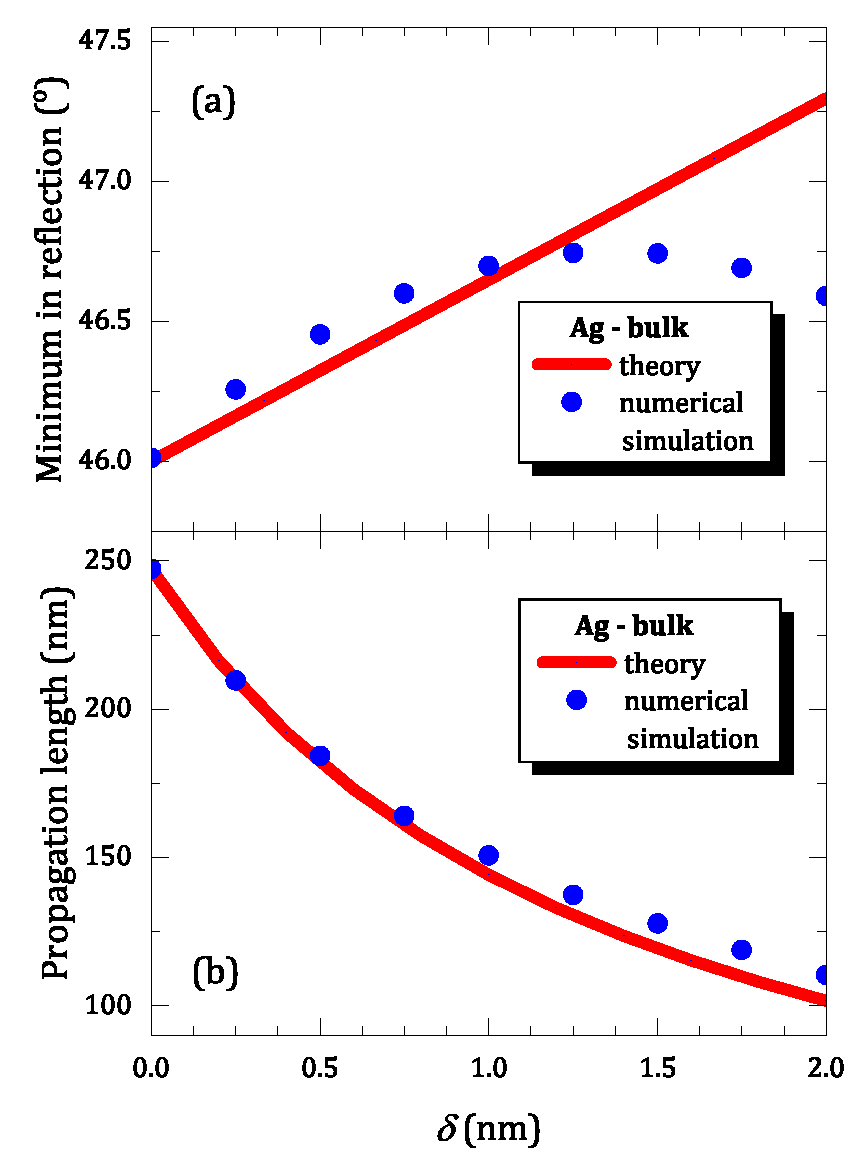
\includegraphics[clip,width=0.48\linewidth]{minpos_bulk.eps}}
\subfloat{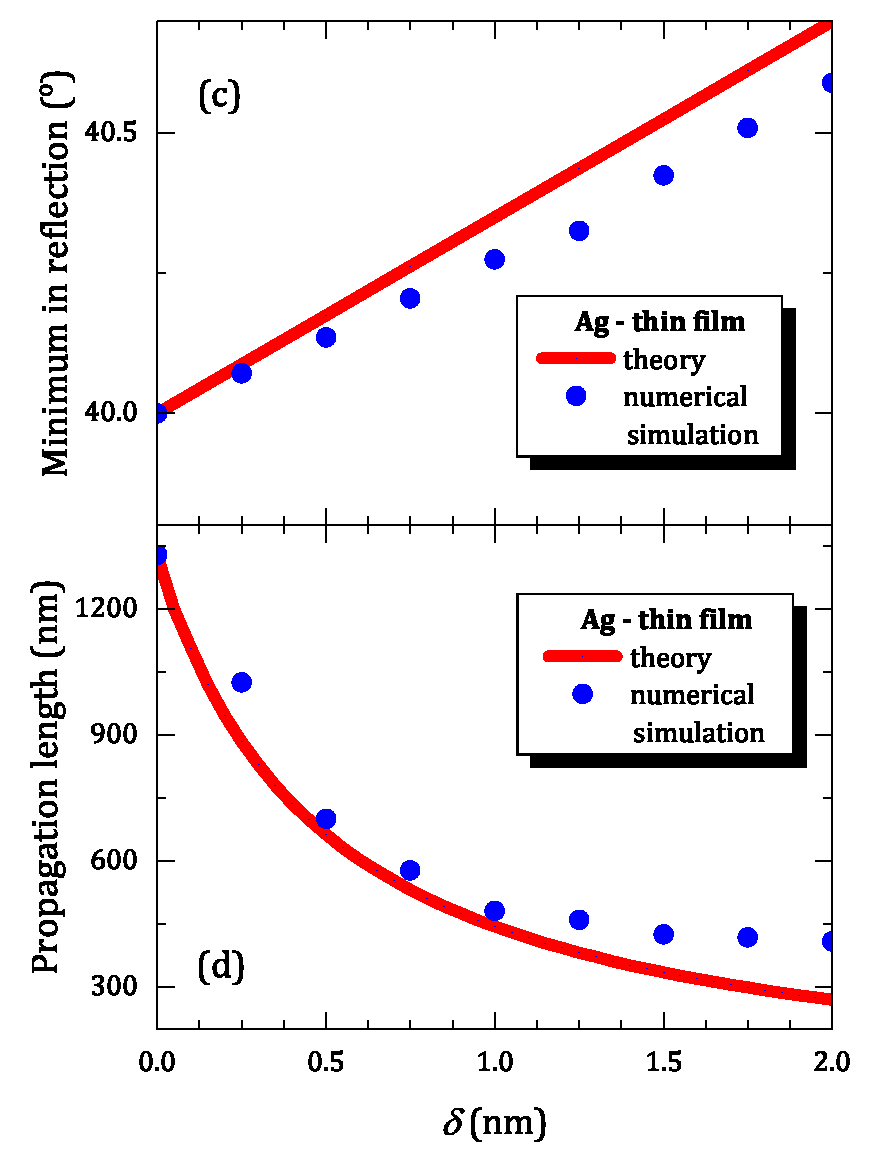
\includegraphics[clip,width=0.48\linewidth]{minpos_thin.eps}}
\caption{Angular positions of the reflected intensity minimum (a,c) and propagation lengths (b,d) for the SPP on the bulk (left panels) and 50nm-thick (right panels) silver slabs as a function of $\delta$. Red curves represent the theoretically calculated dependence and blue data points correspond to the numerical simulations. The results for the ideal interface are included as the data at $\delta=0$.}
\label{fig:minposPlasmon}
\end{figure}

In order to excite the SPP on the air-silver interface, the plasmon wavevector $k=k(\omega)$ must match the parallel to the interface component of the wavevector of the laser light: $k(\omega)=n\omega/c \sin\theta$.
When this condition is satisfied, there will be a minimum in reflection at exactly the direction given by angle $\theta$ (see \cref{fig:ottosetupPlasmon}).
%
For the chosen parameters, the minimum in reflection in the case with bulk sample is observed for $\theta=46.0^{\circ}$, and in the case of  the 50nm-thick film the minimum is at $\theta=40.0^{\circ}$ and $\theta=55.6^{\circ}$ indicating the excitation of the plasmonic mode at the lower (air-silver) interface.

With that, I impose the continuous dielectric permittivity \cref{eq:epsilonContinuous} on the air-silver interfaces and detect how the minimum in reflection shifts its angular position and how the plasmon propagation length changes when varying the parameter $\delta$.

\cref{fig:minposPlasmon} shows the results obtained for both samples.
The minimum in reflection was identified by the angle $\theta$ at which the intensity of the reflected laser light along the circular surface of the prism is the lowest.
As for the propagation length, its evaluation requires extracting the dependence of the SPP intensity on the coordinate along the interface.
The logarithm of the intensity is expected to decay linearly with the distance, which follows from the relation $I(x)=I_0 e^{-2x/L}$.
Then, if one fits a linear function to such data and finds its slope, the propagation length is calculated as $L=-2/\mathrm{slope}$.

The data points from the numerical simulation indicate that the SPP propagation length is significantly reduced when increasing $\delta$, and the minimum in reflection shifts towards the larger angles $\theta$ which means the SPP dispersion shifts towards higher wavevectors $k$ for a given frequency $\omega$.
The same can alternatively be thought of as a red-shift of the SPP eigenfrequencies $\omega$ for a given wavevector $k$.
The theoretical results for the propagation length $L=(2\omega'')^{-1} |d\omega/dk|$ shown in \cref{fig:minposPlasmon} are calculated based on \cref{eq:correctionPlasmonIm}, while the resonant excitation condition $k(\omega)=n\omega/c \sin\theta$ together with \cref{eq:omegatokPlasmon} gives the angular shift $\Delta\theta=\Delta k'/k \tan\theta=-\Delta\omega'/k |d\omega/dk|\tan\theta$.

The theoretical calculations demonstrate good agreement with the numerical data, except for $\delta>1$nm, when the numerically simulated angular position of the minimum actually starts decreasing and the perturbation theory results become invalid.
The reason for it is the strong modification of the SPP spectrum for large $\delta$.
Namely, increasing the SPP damping always implies a reduction of the wavevector of the plasmon at the resonant frequency $\omega_{spp}$, and because of the significant SPP damping due to radiation losses the SPP excitation indeed occurs for smaller incident angle $\theta$.

Another factor to mention is the influence of the prism, which explicitly allows the SPP to leak out through itself and therefore introduces more modifications to the SPP spectrum which are unaccounted for by the~perturbation theory.
In the real experiment, there may also arise additional issues with the sample heating during the SPP excitation, the possible dielectric breakthrough and the charge leakage under influence of the applied DC electric field.

%%%%%%%%%%%%%%%%%%%%%%%%%%%%%%%%%%%%%%%%%%%%%%%%%%%%%%%%%%%%%%%%%%%%
\section{Summary}

This chapter comprises of the comprehensive theoretical and numerical studies of the SPP propagation in layered systems along the interfaces featuring epsilon-near-zero transition regions.
I developed the novel integral approach to the SPP eigenvalue problem, which is then applied to calculate the linear correction to the SPP spectrum.
The obtained correction describes the spectrum difference with respect to the setting with "ideal" interfaces, i.e., where the transition layer is regarded as infinitesimally thin.
I demonstrated that this correction is essentially complex, which means that even in a lossless environment the plasmon acquires a nonzero dissipation rate.
In other words, the critical point within the epsilon-near-zero region opens a new energy decay channel for the SPP.
This decay is due to neither the electron collisions in metal nor the metal surface roughness, as these factors were intentionally eliminated from the system.
However, the SPP now has the possibility to excite the bulk plasmons via the critical point.
The SPP thus eventually radiates its energy away from the interface, and adjusting the transition layer width presents a new means of manipulating the SPP resonant frequency as well as its propagation length.
The obtained general expression for the spectrum correction is valid for the arbitrary dielectric function profile, and the proposed analytical approach may easily be extended to address more complicated geometries, in particular, cylindrical or spherical layered structures.

I also numerically simulated the SPP propagation and excitation on top of the two silver samples --- bulk metal and thin film, ---  and computed the changes to the plasmonic dispersion caused by the smooth transition of the dielectric function between the media.
The theoretical predictions agree well with the numerical simulation for frequencies which are not too close to the SPP resonance.

These findings are of particular importance for designing the plasmonic-based optical devices which employ SPPs for the photon emission enhancement and for near-field imaging applications.

%%% Local Variables: 
%%% mode: latex
%%% TeX-master: "dissertation"
%%% End: 

%%%%%%%%%%%%%%%%%%%%%%%%%%%%%%%%%%%%%%
\chapter{RESULTS AND CONCLUSIONS}
%%%%%%%%%%%%%%%%%%%%%%%%%%%%%%%%%%%%%%

In this dissertation I investigated the~implications of the~physical processes occurring at the~interfaces between media in three different acoustic and electrodynamic systems.
There are two keystones that allow a~comprehensive study of each system and provide insights to the~nature of phenomena occurring in them.
The first one is the analysis of the~band structure together with the~dispersion relation of the systems, and the other one is the~calculation of the~transmission properties that requires solving the~inhomogeneous problem.

For the~two acoustic systems --- the~fluid channel between two solid plates and the~periodic chain of perforated metallic cylindrical shells --- I analytically obtained their transmission spectra and explained the~reasons for anomalously suppressed transmission at certain frequencies, which was experimentally observed previously.
I also demonstrated how these systems can serve as passive antennas, redirecting or splitting the~incident acoustic signal.
The~latter nontrivial effects are enabled by the~surface modes excited at the~interfaces in the~systems: coupled Rayleigh waves in one case and quasi-surface waves confined along the~chain in another case.

For the~metal-dielectric slab having a~realistic interface (essentially being an~ENZ transition layer) I theoretically derived how the~spectrum of the~surface plasmon propagating along such interface is altered by the~presence of the~transition layer and discovered a~new nonradiative mechanism of plasmonic decay which the~plasmon thus unavoidably acquires.
The~numerical simulations that I performed visualized the~excitation of the~surface plasmon inside the~ENZ layer between the~metal and the~dielectric when the~layer thickness was controlled by an~external electrostatic field.
The~results obtained from the~simulations agreed with the~theoretical analysis and helped understand how the~effect can be observed experimentally.

An~interesting question to discuss is whether the~material properties and system geometries can be optimized in order to achieve stronger manifestation of the~described phenomena.
I conclude that in each case one should run a~corresponding optimization procedure to find the~optimal values instead of simply pushing the~material properties to their extremes.
Namely, the~fluid-channel system is able to redirect sound through the~Rayleigh waves, the~existence of which relies on the~coupling between the~fluid and the~solid plates.
If the~density and stiffness of the~solid are significantly increased, the~plates become rigid and no propagation of Rayleigh waves is possible.
In the~other extreme case, when the~impedance of the~solid $\rho c$ is reduced to as low as the~impedance of fluid, the~whole system becomes virtually transparent for incoming sound, which does not facilitate emerging of Rayleigh waves.
The~same goes for the~linear chain of perforated shells: the~sound is redirected via one of the~eigenmodes which would be much more dissipative if the~shells were thicker or with smaller perforations, or would cease to exist for ultrathin shells with large perforations.
The~splitting of sound by the~chain also relies on the~weakness of the~scatterers, since a~better frequency resolution is achieved when the~band gap is narrower, but, again, the~scatterers too weak would not split any noticeable amount of incoming sound.
In both cases changes to other parameters of the~geometry only lead to scaling of the~device operating frequency regions.
As for the~surface plasmon problem, it is desirable to stretch the~transition layer as much as possible (while not causing a~dielectric breakdown) to get stronger modifications of the~plasmonic spectrum, however, the~accompanying nonradiative losses would grow as well, extinguishing the~plasmon before it is even formed.

Overall, I exposed several physical phenomena which are of fundamental significance to physical acoustics and electrodynamics, although they also have immediate value to bring to the~real-world applications by furnishing design ideas for acoustic waveguides and antennas and establishing the~limits of the~plasmonic-based devices.

%%% Local Variables: 
%%% mode: latex
%%% TeX-master: "dissertation"
%%% End: 


%%% Uncomment if there are appendices. This command sets some things up in
%%% preparation for the actual appendices.
\appendix

%%% Include appendix "chapters" here. A single appendix should start with
%%% \appchapter*{TITLE} rather than \chapter{TITLE}. This supresses the 
%%% numbering (if there is only one appendix it doesn't rate a number). If
%%% there is more than one appendix, use \appchapter to get numbered
%%% appendices (A, B, C, ...).  
\renewcommand{\theHchapter}{A\arabic{chapter}}
\appchapter{CHOICE OF THE BRANCH CUT FOR THE COMPLEX-VALUED SQUARE ROOT FUNCTION\label{appBranchCut}}

Here I consider a~general case of a~wave of a~form
\begin{equation}
\label{eq:waveA}
u(x,y,z,t) = u_0 e^{ik_xx+ik_zz-i\omega t}
\end{equation}
propagating in a~homogeneous and isotropic medium in the~semispace $z>0$ bounded by an~interface $z=0$.
Suppose the~dispersion of the~wave is parabolic,
\begin{equation}
\label{eq:dispA}
k_x^2+k_z^2 = \frac{\omega^2}{c_{ph}^2},
\end{equation}
with $c_{ph}$ being the~phase velocity of the~wave.

Now, if the~value of the~$x$-component of the~wave vector, $k_x$, is determined by the~physical process developing in the~medium, one can find the~$z$-component of the~wave vector to be
\begin{equation}
\label{eq:dispkzA}
k_z = \sqrt{\frac{\omega^2}{c_{ph}^2}-k_x^2}.
\end{equation}

If the~value of $k_x$ is real and $k_x < \omega/c_{ph}$, the~value of $k_z$ is then also real, and the~wave \cref{eq:waveA} is a~simple plane wave running in the~direction of $\textbf{k} = (k_x,0,k_z)$.
In the~case of $k_x > \omega/c_{ph}$ the~value of $k_y$ is purely imaginary, $k_z = i\sqrt{k_x^2-\omega^2/c_{ph}^2} = i\kappa_z$, $\kappa_z>0$, which is typical for guided modes that propagate along an~interface in the~$x$-direction and decay in the~perpendicular direction into the~medium:
\begin{equation*}
u(x,y,z,t) = u_0 e^{ik_xx-\kappa_zz-i\omega t}.
\end{equation*}

There are, however, two other possible wave behaviors that are described by the complex-valued $k_x$ and therefore require special attention.
First of all, the~energy carried with the~wave can only dissipate, which corresponds to $\im k_x > 0$, and the~case of $\im k_x < 0$ does not have any physical sense.
This implies that $k_x$ lies in the~first quadrant of the~complex plane, and therefore $k_z^2 = \omega^2/c_{ph}^2-k_x^2$ is in either third or fourth quadrants.
On the~other hand, the~relationship \cref{eq:dispA} dictates that the~signs of the~real and imaginary parts of $k_z$ be opposite (with $k_z$ in the~second or fourth quadrants), otherwise it cannot be satisfied for any given purely real $\omega$ and complex $k_x$ with both $\re k_x > 0$ and $\im k_x > 0$.

For the~positive values of $\re k_z^2$, i.e., when $\re\left(\omega^2/c_{ph}^2-k_x^2\right) > 0$, the~correct behavior of the~wave is the~radiative one, with $\re k_z > 0$, so the~square root should map the~values of $k_z^2$ from the~fourth quadrant into the~fourth quadrant.
Note that $\im k_z > 0$ in this case, which formally means an~exponential growth of the~wave amplitude away from the~interface.
However, the~amplitude decay along the~$x$-axis "compensates" for the~growth along the~$z$-axis \cite{maradudin1,ingerbrigsten,lim}, and, in fact, it can be shown that such a~wave propagates with a~constant amplitude along the~direction of $\mathbf{k'} = (\re k_x,0,\re k_z)$.
This is a~clear manifestation of the~radiative behavior since the~energy of the~wave is not being transmitted along the~interface but is rather carried away at an~angle from it.

For the~negative values of $\re k_z^2$, the~wave must be nonradiative \cite{maradudin2,maradudin3}, with positive $\im k_z$ providing the~exponential decay away from the~interface, and the~corresponding mapping for the~square root function is from the~third into the~second quadrant.

One possibility to satisfy all the~conditions outlined above is to define the~complex-valued square root function with the~branch cut along the~negative imaginary axis.
%
Alternatively, one can use the~conventional square-root function (with the~branch cut along the~negative real axis) and, instead, explicitly specify the~sign ("$+$" or "$-$") in front of the~square root in \cref{eq:dispkzA} in each case.



\appchapter{CALCULATION OF FOURIER TRANSFORMS FOR PROPAGATING AND LEAKY RAYLEIGH EIGENMODES}\label{appRayleigh}

Consider the~integral
\begin{equation}
\label{eq:fourierA}
\CF(k, \varkappa)~=~\frac{e^{\varkappa d/2}}{2}\left(\int\limits_{-\infty}^{-d/2}e^{-ikz+\varkappa z}dz + \int\limits_{+d/2}^{+\infty}e^{-ikz-\varkappa z}dz\right)
\end{equation}
which arises when the~Fourier transforms of \cref{eq:B5Rayleigh}-\cref{eq:B6Rayleigh} are calculated.
If the~parameter $\varkappa$ describes the~propagating Rayleigh eigenmode, i.e., if $\re \varkappa > 0$ and $\im \varkappa = 0$, the~calculation of \cref{eq:fourierA} is trivial:
\begin{align}
\CF(k, \varkappa)~&=~\frac{e^{\varkappa d/2}}{2}\left(\int\limits_{-\infty}^{-d/2}e^{-ikz+\varkappa z}dz + \int\limits_{+d/2}^{+\infty}e^{-ikz-\varkappa z}dz\right)~=\\
&=~\frac{e^{\varkappa d/2}}{2}\int\limits_{+d/2}^{+\infty}\left(e^{+ikz-\varkappa z}+e^{-ikz-\varkappa z}\right)dz~= \notag\\
&=~\frac{e^{\varkappa d/2}}{2}\left(\frac{e^{(ik-\varkappa)d/2}}{\varkappa-ik}+\frac{e^{(-ik-\varkappa)d/2}}{\varkappa+ik}\right)~= \notag\\
&=~\frac{1}{k^2+\varkappa^2}\left(\varkappa \cos\frac{kd}{2}-k\sin\frac{kd}{2}\right). \notag
\end{align}

However, for the~leaky Rayleigh eigenmode with $\re\varkappa < 0$ and $\im\varkappa < 0$ the~integral \cref{eq:fourierA} diverges.
Its value can be written as a~limit
\begin{equation}
\CF(k, \varkappa)~=~\frac{e^{\varkappa d/2}}{2}\left(\frac{e^{(ik-\varkappa)d/2}}{\varkappa-ik}+\frac{e^{(-ik-\varkappa)d/2}}{\varkappa+ik}\right) - \lim\limits_{Z\rightarrow +\infty}\frac{e^{\varkappa d/2}}{2}\left(\frac{e^{(ik-\varkappa)Z/2}}{\varkappa-ik}+\frac{e^{(-ik-\varkappa)Z/2}}{\varkappa+ik}\right).
\end{equation}

It was shown in \cite{jia} that the~divergence can be avoided with the~introduction of perfectly matched layers (PMLs) in the~regions $|z| > L$, where $L$ is a~characteristic distance beyond which the~physical processes are of no interest.
In the~problem of sound transmission through a~fluid channel between two elastic plates, $L$ could be the~size of the~actual plates in the~direction away from the~channel.
Within the~PML the~signal undergoes fast attenuation, and the~PML behavior is typically modeled by a~complex coordinate transform.
Namely, the~integral in the~original limits is split into two parts
\begin{equation}
\int\limits_{d/2}^{+\infty}f(z)dz \rightarrow \int\limits_{d/2}^{L}f(z)dz + \int\limits_{L}^{+\infty}f(z')g(z')dz',
\end{equation}
where the~attenuation in the~PML is added by the~factor $g(z')$, and the~latter integral must be identical to the~integral along the~line in the~complex plane $z$:
\begin{equation}
\int\limits_{L}^{+\infty}f(z')g(z')dz' \equiv \int\limits_{L}^{L+(1+i\alpha)\infty}f(z)dz.
\end{equation}

The~integrands in \cref{eq:fourierA} are analytical functions, so the~contour integral
\begin{equation}
\CF(k, \varkappa)~=~\frac{e^{\varkappa d/2}}{2}\int\limits_{+d/2}^{L+(1+i\alpha)\infty}\left(e^{+ikz-\varkappa z}+e^{-ikz-\varkappa z}\right)dz
\end{equation}
is evaluated to
\begin{equation}
\label{eq:limitA}
\CF(k, \varkappa)~=~\frac{e^{\varkappa d/2}}{2}\left(\frac{e^{(ik-\varkappa)d/2}}{\varkappa-ik}+\frac{e^{(-ik-\varkappa)d/2}}{\varkappa+ik}\right) - \lim\limits_{Z\rightarrow L+(1+i\alpha)\infty}\frac{e^{\varkappa d/2}}{2}\left(\frac{e^{(ik-\varkappa)Z/2}}{\varkappa-ik}+\frac{e^{(-ik-\varkappa)Z/2}}{\varkappa+ik}\right).
\end{equation}
The~value of $\alpha$, which characterizes the~PML, must be chosen to guarantee the~finite value of the~limit in the~latter expression.

For $k \ge 0$ and $\alpha > \left|\re\varkappa/\im\varkappa\right|$ the~limit in \cref{eq:limitA} is zero and
\begin{equation}
\CF(k, \varkappa)~=~\frac{1}{k^2+\varkappa^2}\left(\varkappa \cos\frac{kd}{2}-k\sin\frac{kd}{2}\right).
\end{equation}

The~final result is the~same for negative values of $k$ as well, as the~function $\CF(k,\varkappa)$ is even with respect to its first argument.



\appchapter{GRAF'S ADDITION THEOREM}\label{appGrafTheorem}

Let there be a~triangle formed by the~vectors $\mathbf{r}_j$, $\mathbf{r}_l$, and $\mathbf{R}_{jl} = \mathbf{r}_j - \mathbf{r}_l$ as shown in the~\cref{fig:grafB}.
Suppose that $\mathbf{r}_l$ has the~coordinates $\left(r_l, \varphi_l\right)$ in the~polar coordinate system with the~origin in $O_l$, while $\mathbf{r}_j = \left(r_j, \varphi_j\right)$ and $\mathbf{R}_{jl} = \left(R_{jl}, \vartheta_{jl}\right)$ in the~polar coordinate system with the~origin in $O_j$.

\begin{figure}
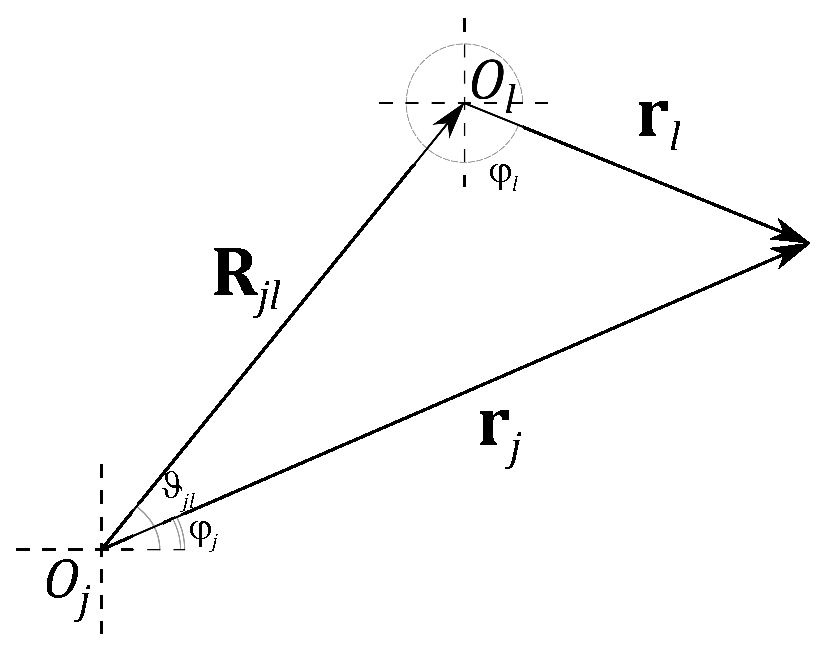
\includegraphics[scale=1]{grafs.eps}
\caption{The~three vectors $\mathbf{r}_j$, $\mathbf{r}_l$, and $\mathbf{R}_{jl}$. The~properties of these vectors can be related using Graf's theorem.}
\label{fig:grafB}
\end{figure}

Then, according to \cite{abramowitz}, the~addition rule exists for the~Hankel functions of the~first kind $H_n$, and it can be written down in the~following form:
\begin{equation}
\label{eq:grafB}
H_n \left(kr_{j}\right) e^{in\left(\varphi_{j}-\vartheta_{jl}\right)} = \sum\limits_{n'=-\infty}^{+\infty} H_{n+n'}\left(kR_{jl}\right) J_{n'}\left(kr_{l}\right) e^{in'\left(\pi-\varphi_{l}+\vartheta_{jl}\right)},
\end{equation}
with the~only restrictions that $j \neq l$ and $r_l < R_{jl}$ \cite{wikiwaves}.
%This theorem is a~special case of a~more general Neumann's addition theorem.



\appchapter{FAST CONVERGING SERIES FOR THE LATTICE SUM}\label{appConvSeries}

The~lattice sum \cref{eq:latticesum}
\begin{equation*}
%\label{A1} 
F(n) = \sum\limits_{l=1}^{+\infty} H_{n}\left(k ld\right) \Big(e^{i q l d} + (-1)^{n} e^{-i q l d}\Big)
\end{equation*}
converges slowly because of the~slow decay $|H_n(kld)| \propto 1/\sqrt{kld}$ of the~Hankel functions for $l \gg 1$.
Nevertheless, the~calculation of this sum is possible since an~equivalent but fast converging representation was found in \cite{twersky}:

\begin{align}
\label{eq:latticesum1C}
F(0) &= -1 -\dfrac{2i}{\pi}\left[\gamma+\ln\dfrac{k}{2p}\right]-\dfrac{2i\left(k^2+2q^2\right)}{p^3 d}\zeta(3)\\
&-\dfrac{2i}{\gamma_0 d}-\dfrac{2i}{d}\sum\limits_{m=1}^{+\infty}\left(\dfrac{1}{\gamma_m}+\dfrac{1}{\gamma_{-m}}-\dfrac{2}{mp}-\dfrac{k^2+2q^2}{m^3 p^3}\right),\notag \\ \notag \\
%
\label{eq:latticesum2C}
F(2n) &= -\dfrac{2i e^{-2in\alpha_0}}{\gamma_0 d} +\dfrac{i}{n\pi} -\dfrac{2i(-1)^n}{\pi}\left(\dfrac{k}{2p}\right)^{2n}\zeta(2n+1)\\
&-2i\sum\limits_{m=1}^{+\infty}\left(\dfrac{e^{-2in\alpha_m}}{\gamma_m d}+\dfrac{e^{2in\alpha_{-m}}}{\gamma_{-m} d}-\dfrac{(-1)^n}{m\pi}\left(\dfrac{k}{2mp}\right)^{2n}\right) \notag \\
&+\dfrac{i}{\pi}\sum\limits_{m=1}^{n}\dfrac{(-1)^m 2^{2m}(n+m-1)!}{(2m)!(n-m)!}\left(\dfrac{p}{k}\right)^{2m} \mathcal{B}_{2m}\left(\dfrac{q}{p}\right), \notag \\ \notag \\
%
\label{eq:latticesum3C}
F(2n-1) &= \dfrac{2i e^{-i(2n-1)\alpha_0}}{\gamma_0 d} +\dfrac{2i(-1)^n qdn}{\pi^2}\left(\dfrac{k}{2p}\right)^{2n-1}\zeta(2n+1)\\
&+2i\sum\limits_{m=1}^{+\infty}\left(\dfrac{e^{-i(2n-1)\alpha_m}}{\gamma_m d}-\dfrac{e^{i(2n-1)\alpha_{-m}}}{\gamma_{-m} d}+\dfrac{i(-1)^n qdn}{m^2\pi^2}\left(\dfrac{k}{2mp}\right)^{2n-1}\right) \notag \\
&-\dfrac{2}{\pi}\sum\limits_{m=0}^{n-1}\dfrac{(-1)^m 2^{2m}(n+m-1)!}{(2m+1)!(n-m-1)!}\left(\dfrac{p}{k}\right)^{2m+1} \mathcal{B}_{2m+1}\left(\dfrac{q}{p}\right). \notag \\ \notag
\end{align}
%
%
Here $\mathcal{B}_m$ is the~Bernoulli polynomial, $\gamma=0.577$ is Euler's constant and
\begin{equation}
p=\dfrac{2\pi}{d}, \qquad
q_m=q+mp, \qquad
\gamma_m=-i\sqrt{k^2-q_m^2}, \qquad
\alpha_m=\arcsin\dfrac{q_m}{k}.
\end{equation}

These representations are valid for $n>0$ and for any complex $k$ with nonnegative imaginary part.
Calculating the~lattice sum for $n<0$ is based on \cref{eq:latticesum2C,eq:latticesum3C} and relies on the~observation that $F_{-n} = (-1)^n F_n$.

When $\im k < 0$, the~original series \cref{eq:latticesum} exponentially diverges.
Nevertheless, since the~expressions \cref{eq:latticesum1C}-\cref{eq:latticesum3C} match the~the~function $F(n)$ for every $k$, $\im k \ge 0$, they can be considered as an~analytic continuation of $F(n)$ to the~lower semispace of the~complex $k$ plane.
Also, in the~case of complex values of $k$, one must identify how the~complex square root in $\gamma_m$ is calculated due to the~concerns outlined in Appendix \ref{appBranchCut}.
The~branch cut for the~square root function in this particular situation must be chosen along the~negative imaginary axis.



\appchapter{IDENTITIES FOR THE DIRAC DELTA FUNCTION\label{appDiracDelta}}

This appendix contains some useful properties of the~Dirac delta function defined as
\begin{equation}
\delta(x)~=~\left\{
\begin{aligned}
+&\infty, &x=0,\\
&0, &x\neq 0,
\end{aligned}\right.
\end{equation}
where additionally
\begin{equation}
\int\limits_{-\infty}^{+\infty}\delta(x)dx~=~1.
\end{equation}
The~following identities exist for the~delta function:
\begin{align}
\label{eq:app_diracdelta1}
f(x_0)~&=~\int\limits_{-\infty}^{+\infty} f(x)\delta(x-x_0)dx,\\
\label{eq:app_diracdelta2}
\delta(x-x_0)~&=~\frac{1}{2\pi} \int\limits_{-\infty}^{+\infty} e^{ip(x-x_0)}dp,
\end{align}
and for its derivative:
\begin{align}
\label{eq:app_diracdelta3}
f'(x_0)~&=~-\int\limits_{-\infty}^{+\infty} f(x)\delta'(x-x_0)dx,\\
\label{eq:app_diracdelta4}
\delta'(x-x_0)~&=~\frac{i}{2\pi} \int\limits_{-\infty}^{+\infty} p e^{ip(x-x_0)}dp,
\end{align}
Here $f(x)$ is an~arbitrary function.
The~identity \eqref{eq:app_diracdelta4} is obtained from \eqref{eq:app_diracdelta2} by calculating its derivative with respect to $x$.



\appchapter{LORENTZ-DRUDE MODEL FIT\\FOR THE DIELECTRIC PERMITTIVITY OF SILVER\label{appSilver}}


In the~generalized Lorentz-Drude model the~material response to the~electric field is given by the~dielectric function
\begin{equation}
\label{app_lorentzdrude}
\epsilon(\omega)~=~\epsilon_{\infty} - \sum\limits_{n=0}^{N}\frac{f_n \omega_p^2}{\omega^2-\omega_{n}^2+i\omega\gamma_n}.
\end{equation}
Here $\epsilon_{\infty}$ is the~limit of the~dielectric permittivity at infinite frequency, $\omega_{n}$ represent the~frequencies of internal resonances, $\gamma_n$ are the~damping rates, and $f_n$ are the~coefficients that scale the~contribution from each term in the~sum.
The~parameters of the~Lorentz-Drude model found in \cite{rakic} provide a~good fit to the~experimental data, in particular, to the~data from \cite{johnson} in the~wavelength range from 0.3$\mu$m to 2.1$\mu$m.

The~best fit parameters are as follows: the~dielectric permittivity is $\epsilon_{\infty}=1$, the~plasma frequency is $\omega_p=9.01$ eV, the~number of terms in the~series is $N=5$, and the~rest of the~parameters are summarized in the~Table~\ref{tab:app_table} below.

\newcolumntype{P}[1]{>{\centering\arraybackslash}p{#1}}

\begin{table}[ht]
\centering
\begin{tabular}{|P{3cm}|P{3cm}|P{3cm}|P{3cm}|}
\hline
$n$ & $\omega_n$ (eV) & $\gamma_n$ (eV) & $f_n$ \\
\hline
0 & 0     & 0.048 & 1     \\ [5pt]
1 & 0.816 & 3.886 & 0.065 \\ [5pt]
2 & 4.481 & 0.452 & 0.124 \\ [5pt]
3 & 8.185 & 0.065 & 0.011 \\ [5pt]
4 & 9.083 & 0.916 & 0.840 \\ [5pt]
5 & 20.29 & 2.419 & 5.646 \\
\hline
\end{tabular}
\caption{Lorentz-Drude model parameters.}
\label{tab:app_table}
\end{table}

Note: the term $\omega_p$ in \cref{app_lorentzdrude} serves as a fitting parameter; it should not be confused with the actual plasma frequency of a conductor which characterizes the density of the valence electrons and their oscillations.
%
%
%
%
%
%\appchapter{CALCULATION OF THE SPP DISPERSION CORRECTION}
%
%The~frequency shift $\Delta\omega = \Delta\omega' - i\Delta\omega''$ is determined from the~condition \cref{eq:correctionPlasmon2}, namely,
%\begin{equation}
%\label{eq:app_correction}
%\frac{\Delta\omega}{\omega_0}~=~\frac{\pi c^2}{\omega_0^2}\frac{\int\limits_{-\infty}^{+\infty} F(p)h_0^*(p)dp}{\int\limits_{-\infty}^{+\infty} |H_0(z)|^2 dz},
%\end{equation}
%where
%\begin{equation}
%\begin{aligned}
%F(p)~&=~\int\limits_{-\infty}^{+\infty} dp'(k^2+pp')\Delta\eta(p-p')h_0(p') = \\
%&=~\frac{1}{2\pi}\int\limits_{-\infty}^{+\infty}dp' (k^2+pp')h_0(p')\left(\int\limits_{-\infty}^{+\infty}dz e^{-i(p-p')z}\left(\frac{1}{\epsilon(z)}-\frac{1}{\epsilon_0(z)}\right)\right) = \\
%&=~\frac{1}{2\pi}\int\limits_{-\infty}^{+\infty}dz \left(\frac{1}{\epsilon(z)}-\frac{1}{\epsilon_0(z)}\right)e^{-ipz} \left(\int\limits_{-\infty}^{+\infty}dp' (k^2+pp')h_0(p') e^{ip'z}\right).
%\end{aligned}
%\end{equation}
%Once the~analytical expression for the~inner integral
%\begin{equation}
%\CF(z,p)~=~\int\limits_{-\infty}^{+\infty}dp' (k^2+pp')h_0(p') e^{ip'z}
%\end{equation}
%is obtained, one can write down the~numerator from \eqref{eq:app_correction} as
%\begin{equation}
%\begin{aligned}
%\int\limits_{-\infty}^{+\infty} F(p)h_0^*(p)dp~&=~\frac{1}{2\pi}\int\limits_{-\infty}^{+\infty} dp\,h_0^*(p) \left( \int\limits_{-\infty}^{+\infty}dz \left(\frac{1}{\epsilon(z)}-\frac{1}{\epsilon_0(z)}\right)e^{-ipz} \CF(z,p)\right)~= \\
%&=~\frac{1}{2\pi} \int\limits_{-\infty}^{+\infty}dz \left(\frac{1}{\epsilon(z)}-\frac{1}{\epsilon_0(z)}\right) \left( \int\limits_{-\infty}^{+\infty} dp\,\CF(z,p) h_0^*(p) e^{-ipz}\right).
%\end{aligned}
%\end{equation}
%Introducing $G(z)=\int\limits_{-\infty}^{+\infty} dp\,\CF(z,p) h_0^*(p) e^{-ipz}$, the~frequency shift $\Delta\omega$ takes the~integral form
%\begin{equation}
%\frac{\Delta\omega}{\omega_0}~=~\frac{c^2}{2\omega_0^2}\frac{\int\limits_{-\infty}^{+\infty}dz \left(\frac{1}{\epsilon(z)}-\frac{1}{\epsilon_0(z)}\right) G(z)}{\int\limits_{-\infty}^{+\infty} |H_0(z)|^2 dz},
%\end{equation}
%which can now be evaluated for any particular choice of the~dielectric function $\epsilon(z)$.
%Moreover, using the~identities for the~Dirac delta function one can analytically integrate the~functions $\CF(z,p)$ and $G(z)$.
%
%Then,
%\begin{align}
%\CF(z,p)~&=~\int\limits_{-\infty}^{+\infty}dp' (k^2+pp')h_0(p') e^{ip'z}~= \\
%&=~\int\limits_{-\infty}^{+\infty}dp' (k^2+pp')e^{ip'z}\left(\frac{1}{2\pi}\int\limits_{-\infty}^{+\infty}dz'H_0(z')e^{-ip'z'}\right)~=\notag\\
%&=~\frac{1}{2\pi} \int\limits_{-\infty}^{+\infty} dz' H_0(z')\left(\int\limits_{-\infty}^{+\infty} dp' (k^2+pp')e^{ip'(z-z')}\right)~=\notag\\
%&=~\int\limits_{-\infty}^{+\infty} dz' H_0(z')\Big(k^2\delta(z-z')+i p \delta'(z-z')\Big)~=~k^2 H_0(z)-ip H_0'(z),\notag
%\end{align}
%and
%\begin{align}
%&G(z)~=~\int\limits_{-\infty}^{+\infty} dp\,\CF(z,p) h_0^*(p) e^{-ipz}~=\\
%&=~\int\limits_{-\infty}^{+\infty}dp \Big(k^2 H_0(z)-ip H_0'(z)\Big)e^{-ipz}\left(\frac{1}{2\pi}\int\limits_{-\infty}^{+\infty} dz'H_0^{*}(z')e^{ipz'}\right)~=\notag\\
%&=~\frac{1}{2\pi} \int\limits_{-\infty}^{+\infty}dz' H_0^{*}(z')\left(k^2H_0(z)\int\limits_{-\infty}^{+\infty}dp\,e^{ip(z-z')} - iH_0'(z) \int\limits_{-\infty}^{+\infty}dp\,pe^{ip(z-z')}\right)~=\notag\\
%&=~\int\limits_{-\infty}^{+\infty}dz' H_0^{*}(z')\Bigg(k^2H_0(z)\delta(z-z')-H_0'(z)\delta'(z-z')\Bigg)~=~k^2|H_0(z)|^2+|H_0'(z)|^2,\notag
%\end{align}
%which allows the~eigenfrequency shift $\Delta\omega$ to take the~form which explicitly depends on the~magnetic field $H_0(z)$ and the~dielectric permittivities $\epsilon_0(z)$ and $\epsilon(z)$ only:
%\begin{equation}
%\label{eq:app_correction2}
%\frac{\Delta\omega}{\omega_0}~=~\frac{c^2}{2\omega_0^2}\frac{\int\limits_{-\infty}^{+\infty}\left(\frac{1}{\epsilon(z)}-\frac{1}{\epsilon_0(z)}\right) \Big(k^2|H_0(z)|^2+|H_0'(z)|^2\Big)dz}{\int\limits_{-\infty}^{+\infty} |H_0(z)|^2 dz}.
%\end{equation}
%
%
%
%
%
%
%\newpage
%\section{The~Single-Interface System}
%
%The~magnetic field of the~unperturbed surface plasmon between two semi-infinite metal and dielectric media has the~following form:
%\begin{equation}
%H_0(z)~=~H_0 \times \left[
%\begin{aligned}
%&e^{-\kappa_d z}, &z>0,\\
%&e^{+\kappa_m z}, &z<0,\\
%\end{aligned}
%\right.
%\end{equation}
%%
%Then
%\begin{equation}
%\frac{1}{2\pi}\int\limits_{-\infty}^{+\infty} |H_0(z)|^2 dz~=~\frac{H_0^2}{4\pi}\left(\frac{1}{\kappa_d}+\frac{1}{\kappa_m}\right).
%\end{equation}
%%
%Inverse Fourier transform of the~magnetic field is
%\begin{equation}
%h_0(p)~=~\frac{1}{2\pi}\int\limits_{-\infty}^{+\infty} H_0(z) e^{-ipz}dz~=~\frac{H_0}{2\pi i}\left(\frac{1}{p-i\kappa_d}-\frac{1}{p+i\kappa_m}\right).
%\end{equation}
%%
%%
%The~integral $\CF(z,p)$ can be calculated analytically:
%\begin{equation}
%\CF(z,p)~=~\int\limits_{-\infty}^{+\infty}dp' (k^2+pp')h_0(p') e^{ip'z}~=~
%H_0\times\left[\begin{aligned}
%&\left(k^2+ip\kappa_d\right)e^{-\kappa_d z}, &z>0,\\
%&\left(k^2-ip\kappa_m\right)e^{+\kappa_m z}, &z<0.
%\end{aligned}\right.
%\end{equation}
%%
%%
%The~latter expression can be further integrated to obtain $G(z)$:
%\begin{equation}
%G(z)~=~\int\limits_{-\infty}^{+\infty} dp\,\CF(z,p) h_0^*(p) e^{-ipz}~=~H_0^2 \times \left[\begin{aligned}
%&\left(k^2+\kappa_d^2\right)e^{-2\kappa_d z}, &z>0,\\
%&\left(k^2+\kappa_m^2\right)e^{+2\kappa_m z}, &z<0.
%\end{aligned}\right.
%\end{equation}

%\appchapter{??? THE DOUBLE-INTERFACE SYSTEM ???\label{appPlasmonFilm}}
%
%%\section{The~Double-Interface System}
%As for the~SPP magnetic field, I write it down as follows:
%\begin{equation}
%\label{eq:app_idealeps2HfieldPlasmon}
%H_0(z)~=~H_0 \times \left[
%\begin{aligned}
%&\CA e^{-\kappa_{d+} (z-s)}, &z>+s,\\
%&\CB e^{+\kappa_m z} + \CC e^{-\kappa_m z}, &|z|<s,\\
%&\CD e^{+\kappa_{d-} (z+s)}, &z<-s,\\
%\end{aligned}
%\right.
%\end{equation}
%where the~coefficients $\CA$, $\CB$, $\CC$ and $\CD$ are related through the~boundary conditions at the~interfaces $z=\pm s$.
%The~continuity of $H_0(z)$ and $\epsilon_0^{-1}(z)\dfrac{dH_0}{dz}$ yields
%\begin{align}
%\CA~=~\CB e^{+\kappa_m s} + \CC e^{-\kappa_m s},& \qquad
%-\frac{\kappa_{d+}}{\epsilon_{d+}}\CA~=~\frac{\kappa_m}{\epsilon_m}\left(\CB e^{+\kappa_m s} - \CC e^{-\kappa_m s}\right), \\
%\CD~=~\CB e^{-\kappa_m s} + \CC e^{+\kappa_m s},& \qquad
%+\frac{\kappa_{d-}}{\epsilon_{d-}}\CD~=~\frac{\kappa_m}{\epsilon_m}\left(\CB e^{-\kappa_m s} - \CC e^{+\kappa_m s}\right).
%\end{align}
%The~solvability of such homogeneous linear system is guaranteed when the~dispersion equation \cref{eq:idealeps2dispPlasmon} is satisfied, and thus one of the~coefficients can be assigned an~arbitrary value and the~rest will be expressed through it.
%
%The~special case where the~metal film is surrounded by the~same dielectric, $\epsilon_{d+},\epsilon_{d-}=\epsilon_{d}$, requires additional consideration since the~plasmonic modes can be now classified as either even (also called long-range) or odd (short-range) with respect to the~coordinate $z$.
%Their respective dispersion relations and magnetic field profiles \cite{zayats} are summarized in \cref{tab:idealeps2Plasmon}.
%
%\newcolumntype{P}[1]{>{\centering\arraybackslash}p{#1}}
%
%\begin{table}[ht]
%\centering
%\begin{tabular}{|P{2.5cm}|P{7cm}|P{7.5cm}|}
%\hline
% &
%even mode (long-range) &
%odd mode (short-range) \\
%\hline & & \\ [-10pt]
%dispersion relation &
%$\dfrac{\epsilon_m}{\epsilon_d}\dfrac{\kappa_d}{\kappa_m} + \tanh{\kappa_m s} = 0$ &
%$\dfrac{\epsilon_m}{\epsilon_d}\dfrac{\kappa_d}{\kappa_m} + \coth{\kappa_m s} = 0$\\ [10pt]
%\hline & & \\ [-10pt]
%magnetic field &
%$H_0(z) = H_0 \times \left[\begin{aligned}
%&e^{\kappa_d\left(s+z\right)}, &z<-s,\\
%&\frac{\cosh{\kappa_m z}}{\cosh{\kappa_m s}}, &|z| \le s,\\
%&e^{\kappa_d\left(s-z\right)}, &z>+s,
%\end{aligned}\right.$ &
%$H_0(z) = H_0 \times \left[\begin{aligned}
%-&e^{\kappa_d\left(s+z\right)}, &z<-s,\\
%&\frac{\sinh{\kappa_m z}}{\sinh{\kappa_m s}}, &|z| \le s,\\
%&e^{\kappa_d\left(s-z\right)}, &z>+s.
%\end{aligned}\right.$\\ [50pt]
%\hline
%coefficients & 
%$\CD = \CA = 1$ \newline $\CB = \CC = \left(2 \cosh{\kappa_m s}\right)^{-1}$ &
%$\CD = -\CA = 1$ \newline $\CB = -\CC = \left(2 \sinh{\kappa_m s}\right)^{-1}$
%\\
%\hline
%\end{tabular}
%\caption{The~implicit dispersion relations $\omega = \omega(k)$ and the~magnetic fields $H_0(z)$ for the~long- and short-range SPP modes.}
%\label{tab:idealeps2Plasmon}
%\end{table}


%
%The~magnetic field of the~unperturbed surface plasmon on a~thin metal film is written as:
%\begin{equation}
%H_0(z)~=~H_0 \times \left[
%\begin{aligned}
%&\CA e^{-\kappa_{d+} (z-s)}, &z>+s,\\
%&\CB e^{+\kappa_m z} + \CC e^{-\kappa_m z}, &|z|<s,\\
%&\CD e^{+\kappa_{d-} (z+s)}, &z<-s.\\
%\end{aligned}
%\right.
%\end{equation}
%%
%Then
%\begin{equation}
%\frac{1}{2\pi}\int\limits_{-\infty}^{+\infty} |H_0(z)|^2 dz~=~\frac{H_0^2}{4\pi}\left[\frac{\CA^2}{\kappa_{d+}}+\frac{\CD^2}{\kappa_{d-}} + 8\CB\CC s + \frac{2\left(\CB^2+\CC^2\right)\sinh{2\kappa_m s}}{\kappa_m}\right].
%\end{equation}
%%
%Inverse Fourier transform of the~magnetic field is
%\begin{equation}
%\begin{aligned}
%h_0(p)~=&~\frac{1}{2\pi}\int\limits_{-\infty}^{+\infty} H_0(z) e^{-ipz}dz~=~\frac{H_0}{2\pi i}\left[\frac{\CA e^{-ips}}{p-i\kappa_{d+}}-\frac{\CD e^{ips}}{p+i\kappa_{d-}}+\right.\\
%&\left.+\CB\,\frac{e^{i\left(p+i\kappa_m\right)s}-e^{-i\left(p+i\kappa_m\right)s}}{p+i\kappa_m}+\CC\,\frac{e^{i\left(p-i\kappa_m\right)s}-e^{-i\left(p-i\kappa_m\right)s}}{p-i\kappa_m}\right].
%\end{aligned}
%\end{equation}
%% &=~\frac{H_0}{2\pi}\left[-\frac{\CA i e^{-ips}}{p-i\kappa_{d+}}+\frac{2\CB\sin{\left(p+i\kappa_m\right)s}}{p+i\kappa_m}+\frac{2\CC%\sin{\left(p-i\kappa_m\right)s}}{p-i\kappa_m}+\frac{\CD i e^{ips}}{p+i\kappa_{d-}}\right]~= \\
%%
%%
%The~integral $\CF(z,p)$ can be calculated analytically:
%\begin{equation}
%\begin{aligned}
%\CF(z,p)~&=~\int\limits_{-\infty}^{+\infty}dp' (k^2+pp')h_0(p') e^{ip'z} = \\
%&=H_0\times\left[\begin{aligned}
%&\CA\left(k^2+ip\kappa_{d+}\right)e^{\kappa_{d+}(s-z)}, &z>s,\\
%&\CB\left(k^2-ip\kappa_m\right)e^{\kappa_m z}+\CC\left(k^2+ip\kappa_m\right)e^{-\kappa_m z}, &|z| \le s,\\
%&\CD\left(k^2-ip\kappa_{d-}\right)e^{\kappa_{d-}(s+z)}, &z<-s.
%\end{aligned}\right.
%\end{aligned}
%\end{equation}
%%
%%
%The~latter expression can be further integrated to obtain $G(z)$:
%\begin{equation}
%\begin{aligned}
%G(z)~&=~\int\limits_{-\infty}^{+\infty} dp\,\CF(z,p) h_0^*(p) e^{-ipz}~=\\
%&=~\left[\begin{aligned}
%&\CA^2\left(k^2+\kappa_{d+}^2\right)e^{2\kappa_{d+}(s-z)}, &z>+s,\\
%&\left(\CB^2 e^{2\kappa_m s}+\CC^2 e^{-2\kappa_m s}\right)\left(k^2+\kappa_m^2\right) + 2\CB\CC\left(k^2-\kappa_m^2\right), &|z| \le s,\\
%&\CD^2\left(k^2+\kappa_{d-}^2\right)e^{2\kappa_{d-}(s+z)}, &z<-s.
%\end{aligned}\right.
%\end{aligned}
%\end{equation}

%%%%%%%%%%%%%%%%
%%%%%%%%%%%%%%%%


%\begin{equation*}
%\int\limits_{-\infty}^{+\infty} F_1(p)h_0^*(p)dp = \int\limits_{-\infty}^{-h} F_1(p)h_0^*(p)dp + \int\limits_{-h}^{+h} F_1(p)h_0^*(p)dp + \int\limits_{+h}^{+\infty} F_1(p)h_0^*(p)dp =
%\end{equation*}
%\begin{equation*}
%= \frac{H_0}{2\pi}\int\limits_{-\infty}^{+\infty}dp\, h_0^*(p)\left(\int\limits_{-\infty}^{-h}dz \left(\frac{1}{\epsilon(z)}-\frac{1}{\epsilon_0(z)}\right) \left(k^2-ip\kappa_d\right)e^{-ipz+\kappa_d(h+z)}\right) + 
%\end{equation*}
%\begin{equation*}
%+ \frac{H_0}{2\pi}\int\limits_{-\infty}^{+\infty}dp\, h_0^*(p)\left(\int\limits_{-\infty}^{-h}dz \left(\frac{1}{\epsilon(z)}-\frac{1}{\epsilon_0(z)}\right) \frac{\left(k^2-ip\kappa_m\right)e^{-ipz+\kappa_m z}+\left(k^2+ip\kappa_m\right)e^{-ipz-\kappa_m z}}{2\cosh{\kappa_m h}}\right) + 
%\end{equation*}
%\begin{equation*}
%+ \frac{H_0}{2\pi}\int\limits_{-\infty}^{+\infty}dp\, h_0^*(p)\left(\int\limits_{+h}^{+\infty}dz \left(\frac{1}{\epsilon(z)}-\frac{1}{\epsilon_0(z)}\right) \left(k^2+ip\kappa_d\right)e^{-ipz+\kappa_d(h-z)}\right) = 
%\end{equation*}
%\begin{equation*}
%= \frac{H_0}{2\pi}\int\limits_{-\infty}^{-h} dz \left(\frac{1}{\epsilon(z)}-\frac{1}{\epsilon_0(z)}\right)\left(\int\limits_{-\infty}^{+\infty} dp\, h_0^*(p) \left(k^2-ip\kappa_d\right)e^{-ipz+\kappa_d(h+z)}\right) + 
%\end{equation*}
%\begin{equation*}
%+ \frac{H_0}{2\pi}\int\limits_{-\infty}^{-h} dz \left(\frac{1}{\epsilon(z)}-\frac{1}{\epsilon_0(z)}\right)\left(\int\limits_{-\infty}^{+\infty} dp\, h_0^*(p) \frac{\left(k^2-ip\kappa_m\right)e^{-ipz+\kappa_m z}+\left(k^2+ip\kappa_m\right)e^{-ipz-\kappa_m z}}{2\cosh{\kappa_m h}}\right) + 
%\end{equation*}
%\begin{equation*}
%+ \frac{H_0}{2\pi}\int\limits_{+h}^{+\infty} dz \left(\frac{1}{\epsilon(z)}-\frac{1}{\epsilon_0(z)}\right)\left(\int\limits_{-\infty}^{+\infty} dp\, h_0^*(p) \left(k^2+ip\kappa_d\right)e^{-ipz+\kappa_d(h-z)}\right) =
%\end{equation*}
%\begin{equation*}
%= \frac{H_0^2}{2\pi}\left[
%\int\limits_{-\infty}^{-h} dz \left(\frac{1}{\epsilon(z)}-\frac{1}{\epsilon_0(z)}\right)\left(k^2+\kappa_d^2\right)e^{2\kappa_d(h+z)} +
%\right.
%\end{equation*}
%\begin{equation}
%+ \int\limits_{-h}^{+h} dz \left(\frac{1}{\epsilon(z)}-\frac{1}{\epsilon_0(z)}\right) \frac{k^2 \cosh^2{\kappa_m z}+\kappa_m^2 \sinh^2{\kappa_m z}}{\cosh^2{\kappa_m h}} +
%\end{equation}
%\begin{equation*}
%\left.
%+ \int\limits_{+h}^{+\infty} dz \left(\frac{1}{\epsilon(z)}-\frac{1}{\epsilon_0(z)}\right)\left(k^2+\kappa_d^2\right)e^{2\kappa_d(h-z)}
%\right].
%\end{equation*}
%
%Thus,
%\begin{equation*}
%\frac{\Delta\omega}{\omega} = \frac{c^2}{2\omega^2}\left[\frac{1}{\kappa_d} + \frac{\sinh{2\kappa_m h} + 2\kappa_m h}{2\kappa_m \cosh^2{\kappa_m h}}\right]^{-1} \times
%\end{equation*}
%\begin{equation*}
%\times \left[
%\int\limits_{-\infty}^{-h} dz \left(\frac{1}{\epsilon(z)}-\frac{1}{\epsilon_0(z)}\right)\left(k^2+\kappa_d^2\right)e^{2\kappa_d(h+z)} +
%\right.
%\end{equation*}
%\begin{equation*}
%+ \int\limits_{-h}^{+h} dz \left(\frac{1}{\epsilon(z)}-\frac{1}{\epsilon_0(z)}\right) \frac{k^2 \cosh^2{\kappa_m z}+\kappa_m^2 \sinh^2{\kappa_m z}}{\cosh^2{\kappa_m h}} +
%\end{equation*}
%\begin{equation*}
%\left.
%+ \int\limits_{+h}^{+\infty} dz \left(\frac{1}{\epsilon(z)}-\frac{1}{\epsilon_0(z)}\right)\left(k^2+\kappa_d^2\right)e^{2\kappa_d(h-z)}
%\right].
%\end{equation*}
%
%The~real part of $\Delta\omega$ is
%\begin{equation*}
%\frac{\Delta\omega'}{\omega} = \frac{c^2}{2\omega^2}\left[\frac{1}{\kappa_d} + \frac{\sinh{2\kappa_m h} + 2\kappa_m h}{2\kappa_m \cosh^2{\kappa_m h}}\right]^{-1} \times
%\end{equation*}
%\begin{equation*}
%\times \left[
%\textrm{V.P.}\int\limits_{-\infty}^{-h} dz \left(\frac{1}{\epsilon(z)}-\frac{1}{\epsilon_d}\right)\left(k^2+\kappa_d^2\right)e^{2\kappa_d(h+z)} +
%\right.
%\end{equation*}
%\begin{equation*}
%+ \int\limits_{-h}^{+h} dz \left(\frac{1}{\epsilon(z)}-\frac{1}{\epsilon_m}\right) \frac{k^2 \cosh^2{\kappa_m z}+\kappa_m^2 \sinh^2{\kappa_m z}}{\cosh^2{\kappa_m h}} +
%\end{equation*}
%\begin{equation}
%\left.
%+ \textrm{V.P.}\int\limits_{+h}^{+\infty} dz \left(\frac{1}{\epsilon(z)}-\frac{1}{\epsilon_d}\right)\left(k^2+\kappa_d^2\right)e^{2\kappa_d(h-z)}
%\right].
%\end{equation}
%\\
%
%The~imaginary part of $\Delta\omega$ is
%\begin{equation*}
%\frac{\Delta\omega''}{\omega} = \frac{\pi c^2}{2\omega^2}\left(k^2+\kappa_d^2\right)\left[\dfrac{1}{\kappa_d} + \dfrac{\sinh{2\kappa_m h} + 2\kappa_m h}{2\kappa_m \cosh^2{\kappa_m h}}\right]^{-1}\sum\limits_{\sigma=\pm}\left|\underset{z=z_\sigma}{\textrm{res }}\dfrac{e^{-2\kappa_d(|z|-h)}}{\epsilon(z)}\right|,
%\end{equation*}
%or
%\begin{equation}
%\frac{\Delta\omega''}{\omega} = \frac{\pi c^2}{2\omega^2}\left(k^2+\kappa_d^2\right)\left[\dfrac{1}{\kappa_d} + \dfrac{\sinh{2\kappa_m h} + 2\kappa_m h}{2\kappa_m \cosh^2{\kappa_m h}}\right]^{-1}\sum\limits_{\sigma=\pm}\dfrac{e^{-2\kappa_d(|z_\sigma|-h)}}{|\epsilon'(z_\sigma)|}.
%\end{equation}

%%% This starts the backmatter, which so far is only the bibliography.
\backmatter

%%% This modifies some bits of the amsplain bibliography style to conform
%%% with UNT/TGS requirements.
\bibliographystyle{modifiedstyle}

%%% Include the .bib file containing the bibliographic information (in
%%% BiBTeX format...). ``bibliography.bib'' is a descriptive name for a
%%% bibliography file in BiBTeX format.
\bibliography{bibliography}{}


%%% That's all folks!
\end{document}